\documentclass[twoside]{book}

% Packages required by doxygen
\usepackage{fixltx2e}
\usepackage{calc}
\usepackage{doxygen}
\usepackage[export]{adjustbox} % also loads graphicx
\usepackage{graphicx}
\usepackage[utf8]{inputenc}
\usepackage{makeidx}
\usepackage{multicol}
\usepackage{multirow}
\PassOptionsToPackage{warn}{textcomp}
\usepackage{textcomp}
\usepackage[nointegrals]{wasysym}
\usepackage[table]{xcolor}

% Font selection
\usepackage[T1]{fontenc}
\usepackage[scaled=.90]{helvet}
\usepackage{courier}
\usepackage{amssymb}
\usepackage{sectsty}
\renewcommand{\familydefault}{\sfdefault}
\allsectionsfont{%
  \fontseries{bc}\selectfont%
  \color{darkgray}%
}
\renewcommand{\DoxyLabelFont}{%
  \fontseries{bc}\selectfont%
  \color{darkgray}%
}
\newcommand{\+}{\discretionary{\mbox{\scriptsize$\hookleftarrow$}}{}{}}

% Page & text layout
\usepackage{geometry}
\geometry{%
  a4paper,%
  top=2.5cm,%
  bottom=2.5cm,%
  left=2.5cm,%
  right=2.5cm%
}
\tolerance=750
\hfuzz=15pt
\hbadness=750
\setlength{\emergencystretch}{15pt}
\setlength{\parindent}{0cm}
\setlength{\parskip}{0.2cm}
\makeatletter
\renewcommand{\paragraph}{%
  \@startsection{paragraph}{4}{0ex}{-1.0ex}{1.0ex}{%
    \normalfont\normalsize\bfseries\SS@parafont%
  }%
}
\renewcommand{\subparagraph}{%
  \@startsection{subparagraph}{5}{0ex}{-1.0ex}{1.0ex}{%
    \normalfont\normalsize\bfseries\SS@subparafont%
  }%
}
\makeatother

% Headers & footers
\usepackage{fancyhdr}
\pagestyle{fancyplain}
\fancyhead[LE]{\fancyplain{}{\bfseries\thepage}}
\fancyhead[CE]{\fancyplain{}{}}
\fancyhead[RE]{\fancyplain{}{\bfseries\leftmark}}
\fancyhead[LO]{\fancyplain{}{\bfseries\rightmark}}
\fancyhead[CO]{\fancyplain{}{}}
\fancyhead[RO]{\fancyplain{}{\bfseries\thepage}}
\fancyfoot[LE]{\fancyplain{}{}}
\fancyfoot[CE]{\fancyplain{}{}}
\fancyfoot[RE]{\fancyplain{}{\bfseries\scriptsize Generated on Fri Apr 1 2016 16\+:47\+:06 for Cellular\+Cryptography by Doxygen }}
\fancyfoot[LO]{\fancyplain{}{\bfseries\scriptsize Generated on Fri Apr 1 2016 16\+:47\+:06 for Cellular\+Cryptography by Doxygen }}
\fancyfoot[CO]{\fancyplain{}{}}
\fancyfoot[RO]{\fancyplain{}{}}
\renewcommand{\footrulewidth}{0.4pt}
\renewcommand{\chaptermark}[1]{%
  \markboth{#1}{}%
}
\renewcommand{\sectionmark}[1]{%
  \markright{\thesection\ #1}%
}

% Indices & bibliography
\usepackage{natbib}
\usepackage[titles]{tocloft}
\setcounter{tocdepth}{3}
\setcounter{secnumdepth}{5}
\makeindex

% Hyperlinks (required, but should be loaded last)
\usepackage{ifpdf}
\ifpdf
  \usepackage[pdftex,pagebackref=true]{hyperref}
\else
  \usepackage[ps2pdf,pagebackref=true]{hyperref}
\fi
\hypersetup{%
  colorlinks=true,%
  linkcolor=blue,%
  citecolor=blue,%
  unicode%
}

% Custom commands
\newcommand{\clearemptydoublepage}{%
  \newpage{\pagestyle{empty}\cleardoublepage}%
}


%===== C O N T E N T S =====

\begin{document}

% Titlepage & ToC
\hypersetup{pageanchor=false,
             bookmarks=true,
             bookmarksnumbered=true,
             pdfencoding=unicode
            }
\pagenumbering{roman}
\begin{titlepage}
\vspace*{7cm}
\begin{center}%
{\Large Cellular\+Cryptography }\\
\vspace*{1cm}
{\large Generated by Doxygen 1.8.10}\\
\vspace*{0.5cm}
{\small Fri Apr 1 2016 16:47:06}\\
\end{center}
\end{titlepage}
\clearemptydoublepage
\tableofcontents
\clearemptydoublepage
\pagenumbering{arabic}
\hypersetup{pageanchor=true}

%--- Begin generated contents ---
\chapter{Namespace Index}
\section{Packages}
Here are the packages with brief descriptions (if available)\+:\begin{DoxyCompactList}
\item\contentsline{section}{\hyperlink{namespace_cellular}{Cellular} }{\pageref{namespace_cellular}}{}
\item\contentsline{section}{\hyperlink{namespace_crypto}{Crypto} }{\pageref{namespace_crypto}}{}
\item\contentsline{section}{\hyperlink{namespace_program}{Program} }{\pageref{namespace_program}}{}
\item\contentsline{section}{\hyperlink{namespace_program_1_1_properties}{Program.\+Properties} }{\pageref{namespace_program_1_1_properties}}{}
\item\contentsline{section}{\hyperlink{namespace_testing}{Testing} }{\pageref{namespace_testing}}{}
\item\contentsline{section}{\hyperlink{namespace_user_forms}{User\+Forms} }{\pageref{namespace_user_forms}}{}
\end{DoxyCompactList}

\chapter{Hierarchical Index}
\section{Class Hierarchy}
This inheritance list is sorted roughly, but not completely, alphabetically\+:\begin{DoxyCompactList}
\item \contentsline{section}{User\+Forms.\+Adapter}{\pageref{class_user_forms_1_1_adapter}}{}
\item \contentsline{section}{Testing.\+Automata\+Test}{\pageref{class_testing_1_1_automata_test}}{}
\item \contentsline{section}{Testing.\+Binary\+Range\+N\+Test}{\pageref{class_testing_1_1_binary_range_n_test}}{}
\item \contentsline{section}{Cellular.\+Cellular\+Automaton}{\pageref{class_cellular_1_1_cellular_automaton}}{}
\begin{DoxyCompactList}
\item \contentsline{section}{Cellular.\+Automaton1\+D}{\pageref{class_cellular_1_1_automaton1_d}}{}
\begin{DoxyCompactList}
\item \contentsline{section}{Cellular.\+Binary1\+D\+Automaton}{\pageref{class_cellular_1_1_binary1_d_automaton}}{}
\begin{DoxyCompactList}
\item \contentsline{section}{Cellular.\+Binary\+Range\+Automaton}{\pageref{class_cellular_1_1_binary_range_automaton}}{}
\begin{DoxyCompactList}
\item \contentsline{section}{Cellular.\+Binary\+Range\+Cyclic\+Automaton}{\pageref{class_cellular_1_1_binary_range_cyclic_automaton}}{}
\end{DoxyCompactList}
\item \contentsline{section}{Cellular.\+Elementary\+Automaton}{\pageref{class_cellular_1_1_elementary_automaton}}{}
\begin{DoxyCompactList}
\item \contentsline{section}{Cellular.\+Elementary\+Fast\+Automaton}{\pageref{class_cellular_1_1_elementary_fast_automaton}}{}
\end{DoxyCompactList}
\item \contentsline{section}{Cellular.\+Reversible\+Automaton}{\pageref{class_cellular_1_1_reversible_automaton}}{}
\end{DoxyCompactList}
\item \contentsline{section}{Cellular.\+Nary1\+D\+Automaton}{\pageref{class_cellular_1_1_nary1_d_automaton}}{}
\begin{DoxyCompactList}
\item \contentsline{section}{Cellular.\+Nary\+Totalistic\+Automaton}{\pageref{class_cellular_1_1_nary_totalistic_automaton}}{}
\begin{DoxyCompactList}
\item \contentsline{section}{Cellular.\+Nary\+Totalistic\+Cyclic\+Automaton}{\pageref{class_cellular_1_1_nary_totalistic_cyclic_automaton}}{}
\end{DoxyCompactList}
\end{DoxyCompactList}
\end{DoxyCompactList}
\item \contentsline{section}{Cellular.\+Automaton2\+D}{\pageref{class_cellular_1_1_automaton2_d}}{}
\begin{DoxyCompactList}
\item \contentsline{section}{Cellular.\+Binary2\+D\+Automaton}{\pageref{class_cellular_1_1_binary2_d_automaton}}{}
\begin{DoxyCompactList}
\item \contentsline{section}{Cellular.\+Totalistic2\+D\+Automaton}{\pageref{class_cellular_1_1_totalistic2_d_automaton}}{}
\begin{DoxyCompactList}
\item \contentsline{section}{Cellular.\+Totalistic2\+D\+Automaton\+Interactive}{\pageref{class_cellular_1_1_totalistic2_d_automaton_interactive}}{}
\end{DoxyCompactList}
\end{DoxyCompactList}
\end{DoxyCompactList}
\end{DoxyCompactList}
\item \contentsline{section}{Cryptography\+Unit\+Tests.\+Common\+Part}{\pageref{class_cryptography_unit_tests_1_1_common_part}}{}
\item \contentsline{section}{Testing.\+Elementary\+Time\+Measure}{\pageref{class_testing_1_1_elementary_time_measure}}{}
\item \contentsline{section}{Cryptography\+Unit\+Tests.\+Encrypter\+Reversible\+C\+Atests}{\pageref{class_cryptography_unit_tests_1_1_encrypter_reversible_c_atests}}{}
\item \contentsline{section}{Cryptography\+Unit\+Tests.\+Encrypter\+Stream\+C\+Atests}{\pageref{class_cryptography_unit_tests_1_1_encrypter_stream_c_atests}}{}
\item \contentsline{section}{Crypto.\+Encrypter\+Wrapper}{\pageref{class_crypto_1_1_encrypter_wrapper}}{}
\item \contentsline{section}{Crypto.\+Export}{\pageref{class_crypto_1_1_export}}{}
\item \contentsline{section}{Crypto.\+Factory}{\pageref{class_crypto_1_1_factory}}{}
\item \contentsline{section}{Testing.\+Factory\+Test}{\pageref{class_testing_1_1_factory_test}}{}
\item Form\begin{DoxyCompactList}
\item \contentsline{section}{Program.\+Crypto\+Form}{\pageref{class_program_1_1_crypto_form}}{}
\item \contentsline{section}{User\+Forms.\+Demo\+Form}{\pageref{class_user_forms_1_1_demo_form}}{}
\end{DoxyCompactList}
\item \contentsline{section}{Crypto.\+Function\+Testing}{\pageref{class_crypto_1_1_function_testing}}{}
\item \contentsline{section}{Crypto.\+Function\+Tests\+For\+Thesis}{\pageref{class_crypto_1_1_function_tests_for_thesis}}{}
\item \contentsline{section}{Testing.\+Function\+Test\+Test}{\pageref{class_testing_1_1_function_test_test}}{}
\item \contentsline{section}{Testing.\+Genetic\+Test}{\pageref{class_testing_1_1_genetic_test}}{}
\item \contentsline{section}{Cellular.\+I\+Binary\+C\+A}{\pageref{interface_cellular_1_1_i_binary_c_a}}{}
\begin{DoxyCompactList}
\item \contentsline{section}{Cellular.\+Binary1\+D\+Automaton}{\pageref{class_cellular_1_1_binary1_d_automaton}}{}
\item \contentsline{section}{Cellular.\+Binary2\+D\+Automaton}{\pageref{class_cellular_1_1_binary2_d_automaton}}{}
\end{DoxyCompactList}
\item \contentsline{section}{Crypto.\+I\+Encrypter}{\pageref{interface_crypto_1_1_i_encrypter}}{}
\begin{DoxyCompactList}
\item \contentsline{section}{Crypto.\+Encrypter\+Reversible\+C\+A}{\pageref{class_crypto_1_1_encrypter_reversible_c_a}}{}
\item \contentsline{section}{Crypto.\+Encrypter\+Stream\+C\+A}{\pageref{class_crypto_1_1_encrypter_stream_c_a}}{}
\end{DoxyCompactList}
\item I\+Enumerable\begin{DoxyCompactList}
\item \contentsline{section}{Cellular.\+Utilities.\+All\+Binary\+Sequences}{\pageref{class_cellular_1_1_utilities_1_1_all_binary_sequences}}{}
\end{DoxyCompactList}
\item \contentsline{section}{Crypto.\+I\+Key\+Extender}{\pageref{interface_crypto_1_1_i_key_extender}}{}
\begin{DoxyCompactList}
\item \contentsline{section}{Crypto.\+Key\+Extender\+Abstract\+D}{\pageref{class_crypto_1_1_key_extender_abstract_d}}{}
\begin{DoxyCompactList}
\item \contentsline{section}{Crypto.\+Key\+Extender\+Copy}{\pageref{class_crypto_1_1_key_extender_copy}}{}
\item \contentsline{section}{Crypto.\+Key\+Extender\+Interlaced}{\pageref{class_crypto_1_1_key_extender_interlaced}}{}
\item \contentsline{section}{Crypto.\+Key\+Extender\+Simple\+Linear}{\pageref{class_crypto_1_1_key_extender_simple_linear}}{}
\item \contentsline{section}{Crypto.\+Key\+Extender\+Simple\+Quadratic}{\pageref{class_crypto_1_1_key_extender_simple_quadratic}}{}
\end{DoxyCompactList}
\item \contentsline{section}{Crypto.\+Key\+Extender\+Abstract\+N}{\pageref{class_crypto_1_1_key_extender_abstract_n}}{}
\begin{DoxyCompactList}
\item \contentsline{section}{Crypto.\+Key\+Extender\+Cheating}{\pageref{class_crypto_1_1_key_extender_cheating}}{}
\item \contentsline{section}{Crypto.\+Key\+Extender\+Genetic}{\pageref{class_crypto_1_1_key_extender_genetic}}{}
\item \contentsline{section}{Crypto.\+Key\+Extender\+Uncertain}{\pageref{class_crypto_1_1_key_extender_uncertain}}{}
\end{DoxyCompactList}
\end{DoxyCompactList}
\item \contentsline{section}{Testing.\+Implementation2\+Test}{\pageref{class_testing_1_1_implementation2_test}}{}
\item Invalid\+Operation\+Exception\begin{DoxyCompactList}
\item \contentsline{section}{Crypto.\+Cannot\+Generate\+Exception}{\pageref{class_crypto_1_1_cannot_generate_exception}}{}
\end{DoxyCompactList}
\item \contentsline{section}{Testing.\+Main\+Tests}{\pageref{class_testing_1_1_main_tests}}{}
\item \contentsline{section}{Program.\+Program}{\pageref{class_program_1_1_program}}{}
\item \contentsline{section}{Program}{\pageref{class_program}}{}
\item \contentsline{section}{Crypto.\+Randomness\+Testing}{\pageref{class_crypto_1_1_randomness_testing}}{}
\item \contentsline{section}{Testing.\+Random\+Test\+Test}{\pageref{class_testing_1_1_random_test_test}}{}
\item \contentsline{section}{Testing.\+Reversible\+Test}{\pageref{class_testing_1_1_reversible_test}}{}
\item \contentsline{section}{Testing.\+Search\+Longest}{\pageref{class_testing_1_1_search_longest}}{}
\item \contentsline{section}{Crypto.\+Search\+S\+G\+A}{\pageref{class_crypto_1_1_search_s_g_a}}{}
\item \contentsline{section}{Testing.\+Totalistic\+Ternary\+Test}{\pageref{class_testing_1_1_totalistic_ternary_test}}{}
\item \contentsline{section}{Cellular.\+Utilities}{\pageref{class_cellular_1_1_utilities}}{}
\item \contentsline{section}{Testing.\+Utility\+Test}{\pageref{class_testing_1_1_utility_test}}{}
\end{DoxyCompactList}

\chapter{Class Index}
\section{Class List}
Here are the classes, structs, unions and interfaces with brief descriptions\+:\begin{DoxyCompactList}
\item\contentsline{section}{\hyperlink{class_user_forms_1_1_adapter}{User\+Forms.\+Adapter} \\*Static class that allows to display an interactive window from a console application. }{\pageref{class_user_forms_1_1_adapter}}{}
\item\contentsline{section}{\hyperlink{class_cellular_1_1_utilities_1_1_all_binary_sequences}{Cellular.\+Utilities.\+All\+Binary\+Sequences} \\*Class for enumerating all binary sequences of a given length. Starting from 00...00, ending at 11...11. }{\pageref{class_cellular_1_1_utilities_1_1_all_binary_sequences}}{}
\item\contentsline{section}{\hyperlink{class_testing_1_1_automata_test}{Testing.\+Automata\+Test} }{\pageref{class_testing_1_1_automata_test}}{}
\item\contentsline{section}{\hyperlink{class_cellular_1_1_automaton1_d}{Cellular.\+Automaton1\+D} \\*Abstract class for all 1\+D automata (binary \& others). }{\pageref{class_cellular_1_1_automaton1_d}}{}
\item\contentsline{section}{\hyperlink{class_cellular_1_1_automaton2_d}{Cellular.\+Automaton2\+D} \\*Abstract class for all 2\+D automata. When indexing, (\char`\"{}height first\char`\"{}) the distance from the top comes before the distance from the left border. }{\pageref{class_cellular_1_1_automaton2_d}}{}
\item\contentsline{section}{\hyperlink{class_cellular_1_1_binary1_d_automaton}{Cellular.\+Binary1\+D\+Automaton} \\*Class containing base-\/constructors for all binary 1\+D automata and implementation of the {\ttfamily \hyperlink{interface_cellular_1_1_i_binary_c_a}{I\+Binary\+C\+A}} interface. The state is kept in a {\ttfamily Bit\+Array}. }{\pageref{class_cellular_1_1_binary1_d_automaton}}{}
\item\contentsline{section}{\hyperlink{class_cellular_1_1_binary2_d_automaton}{Cellular.\+Binary2\+D\+Automaton} \\*Class containing base-\/constructors for all binary 2\+D automata and implementation of the {\ttfamily \hyperlink{interface_cellular_1_1_i_binary_c_a}{I\+Binary\+C\+A}} interface. The state is kept in an array of {\ttfamily Bit\+Array}s reprezenting rows. }{\pageref{class_cellular_1_1_binary2_d_automaton}}{}
\item\contentsline{section}{\hyperlink{class_cellular_1_1_binary_range_automaton}{Cellular.\+Binary\+Range\+Automaton} \\*Class representing any binary 1\+D automaton with symmetric scope. The automaton has firmly set borders. Referencing a cell beyond borders acts as referencing a dead cell. }{\pageref{class_cellular_1_1_binary_range_automaton}}{}
\item\contentsline{section}{\hyperlink{class_cellular_1_1_binary_range_cyclic_automaton}{Cellular.\+Binary\+Range\+Cyclic\+Automaton} \\*Class representing any binary 1\+D automaton with symmetric scope. The automaton is cyclic -\/ its edges are connected. Therefore, all positions are equivalent. }{\pageref{class_cellular_1_1_binary_range_cyclic_automaton}}{}
\item\contentsline{section}{\hyperlink{class_testing_1_1_binary_range_n_test}{Testing.\+Binary\+Range\+N\+Test} \\*Simple demonstration that {\ttfamily Binary\+Range\+Automaton} can be used in a place of {\ttfamily Elementary\+Automaton}. }{\pageref{class_testing_1_1_binary_range_n_test}}{}
\item\contentsline{section}{\hyperlink{class_crypto_1_1_cannot_generate_exception}{Crypto.\+Cannot\+Generate\+Exception} \\*Custom exception that any key extender can throw. }{\pageref{class_crypto_1_1_cannot_generate_exception}}{}
\item\contentsline{section}{\hyperlink{class_cellular_1_1_cellular_automaton}{Cellular.\+Cellular\+Automaton} \\*The top class of the C\+A hierarchy. Every constructor should follow this logical order when considering its parametres\+: specification of the type (usually not needed), rule, size, initial state / rng. }{\pageref{class_cellular_1_1_cellular_automaton}}{}
\item\contentsline{section}{\hyperlink{class_program_1_1_crypto_form}{Program.\+Crypto\+Form} \\*Windows application for users who want to encrypt their data using a cellular automata based algorithm. }{\pageref{class_program_1_1_crypto_form}}{}
\item\contentsline{section}{\hyperlink{class_user_forms_1_1_demo_form}{User\+Forms.\+Demo\+Form} \\*Interactive visual demo of the Game of Life on a rectangular playground. This is not a platform for programming or serious experiments. }{\pageref{class_user_forms_1_1_demo_form}}{}
\item\contentsline{section}{\hyperlink{class_cellular_1_1_elementary_automaton}{Cellular.\+Elementary\+Automaton} \\*Class representing 256 elementary C\+A with firmly set borders. This specific implementation calculates every bit separately. }{\pageref{class_cellular_1_1_elementary_automaton}}{}
\item\contentsline{section}{\hyperlink{class_cellular_1_1_elementary_fast_automaton}{Cellular.\+Elementary\+Fast\+Automaton} \\*Class representing 256 elementary C\+A with firmly set borders. This specific implementation maps 10 cells onto 8 cells at once, so it should be faster a little. }{\pageref{class_cellular_1_1_elementary_fast_automaton}}{}
\item\contentsline{section}{\hyperlink{class_testing_1_1_elementary_time_measure}{Testing.\+Elementary\+Time\+Measure} \\*Simple test of how different classes are (in)efficient for implementing elementary C\+A rules. }{\pageref{class_testing_1_1_elementary_time_measure}}{}
\item\contentsline{section}{\hyperlink{class_crypto_1_1_export}{Crypto.\+Export} \\*Public static class that gives access to our cryptographical tools. Can be used from any assembly. }{\pageref{class_crypto_1_1_export}}{}
\item\contentsline{section}{\hyperlink{class_crypto_1_1_factory}{Crypto.\+Factory} \\*\hyperlink{class_crypto_1_1_factory}{Factory} class containing methods for building cellular automata and key extenders from textual description. Sometimes used together with {\ttfamily Cellular\+Automaton.\+Tell\+Type()} resp. {\ttfamily I\+Binary\+C\+A.\+Tell\+Type()} method as a replacement for missing serialization / deserialization features. }{\pageref{class_crypto_1_1_factory}}{}
\item\contentsline{section}{\hyperlink{class_testing_1_1_factory_test}{Testing.\+Factory\+Test} }{\pageref{class_testing_1_1_factory_test}}{}
\item\contentsline{section}{\hyperlink{class_crypto_1_1_function_testing}{Crypto.\+Function\+Testing} \\*Class for testing properties of key extending algorithms. }{\pageref{class_crypto_1_1_function_testing}}{}
\item\contentsline{section}{\hyperlink{class_crypto_1_1_function_tests_for_thesis}{Crypto.\+Function\+Tests\+For\+Thesis} \\*Wrapper for class {\ttfamily \hyperlink{class_crypto_1_1_function_testing}{Function\+Testing}}. It generates results in the form, which is suitable for my thesis. }{\pageref{class_crypto_1_1_function_tests_for_thesis}}{}
\item\contentsline{section}{\hyperlink{class_testing_1_1_function_test_test}{Testing.\+Function\+Test\+Test} \\*Simple demonstration of utilities for C\+A. }{\pageref{class_testing_1_1_function_test_test}}{}
\item\contentsline{section}{\hyperlink{class_testing_1_1_genetic_test}{Testing.\+Genetic\+Test} }{\pageref{class_testing_1_1_genetic_test}}{}
\item\contentsline{section}{\hyperlink{interface_cellular_1_1_i_binary_c_a}{Cellular.\+I\+Binary\+C\+A} \\*Common interface for all binary cellular automata. Most work with C\+A is done through this interface. Only subclasses of {\ttfamily \hyperlink{class_cellular_1_1_cellular_automaton}{Cellular\+Automaton}} are supposed to implement this interface. }{\pageref{interface_cellular_1_1_i_binary_c_a}}{}
\item\contentsline{section}{\hyperlink{interface_crypto_1_1_i_key_extender}{Crypto.\+I\+Key\+Extender} \\*Interface for all algorithms that can perform key stretching. Can be used from any assembly. }{\pageref{interface_crypto_1_1_i_key_extender}}{}
\item\contentsline{section}{\hyperlink{class_testing_1_1_implementation2_test}{Testing.\+Implementation2\+Test} \\*Simple demonstration that {\ttfamily Elementary\+Automaton} and {\ttfamily Elementary\+Fast\+Automaton} do the same thing. }{\pageref{class_testing_1_1_implementation2_test}}{}
\item\contentsline{section}{\hyperlink{class_crypto_1_1_key_extender_abstract_d}{Crypto.\+Key\+Extender\+Abstract\+D} \\*Abstract class for all key extenders that implement \hyperlink{class_crypto_1_1_key_extender_abstract_d_ae403b92e9038b9c0bc7a21885e24ffc7}{Double\+Key()}. Method \hyperlink{class_crypto_1_1_key_extender_abstract_d_a3ec7fa96f391d840043eff0c8409d130}{Extend\+Key()} is provided (iterates \hyperlink{class_crypto_1_1_key_extender_abstract_d_ae403b92e9038b9c0bc7a21885e24ffc7}{Double\+Key()} method until we get a desired length). }{\pageref{class_crypto_1_1_key_extender_abstract_d}}{}
\item\contentsline{section}{\hyperlink{class_crypto_1_1_key_extender_abstract_n}{Crypto.\+Key\+Extender\+Abstract\+N} \\*Abstract class for all key extenders that implement \hyperlink{class_crypto_1_1_key_extender_abstract_n_a9df4156ad0a84730f87119e5a25cf1ef}{Extend\+Key()}. Method \hyperlink{class_crypto_1_1_key_extender_abstract_n_a57e9a8247ebde9e639c16107c2961d10}{Double\+Key()} simply calls \hyperlink{class_crypto_1_1_key_extender_abstract_n_a9df4156ad0a84730f87119e5a25cf1ef}{Extend\+Key()}. }{\pageref{class_crypto_1_1_key_extender_abstract_n}}{}
\item\contentsline{section}{\hyperlink{class_crypto_1_1_key_extender_cheating}{Crypto.\+Key\+Extender\+Cheating} \\*Fake key extender which only generates random long key independently of the short key. }{\pageref{class_crypto_1_1_key_extender_cheating}}{}
\item\contentsline{section}{\hyperlink{class_crypto_1_1_key_extender_copy}{Crypto.\+Key\+Extender\+Copy} \\*Stupid key extender which only copies the input (repeatedly). }{\pageref{class_crypto_1_1_key_extender_copy}}{}
\item\contentsline{section}{\hyperlink{class_crypto_1_1_key_extender_genetic}{Crypto.\+Key\+Extender\+Genetic} \\*Algorithms which runs a genetic algorithm to find the best sequence of extenders for each key. Generating the long key may take a very long time. }{\pageref{class_crypto_1_1_key_extender_genetic}}{}
\item\contentsline{section}{\hyperlink{class_crypto_1_1_key_extender_interlaced}{Crypto.\+Key\+Extender\+Interlaced} \\*Different linear algorithm, which uses specified number of steps of the underlying C\+A. }{\pageref{class_crypto_1_1_key_extender_interlaced}}{}
\item\contentsline{section}{\hyperlink{class_crypto_1_1_key_extender_simple_linear}{Crypto.\+Key\+Extender\+Simple\+Linear} \\*Simple algorithm, which uses only two steps of the underlying C\+A. }{\pageref{class_crypto_1_1_key_extender_simple_linear}}{}
\item\contentsline{section}{\hyperlink{class_crypto_1_1_key_extender_simple_quadratic}{Crypto.\+Key\+Extender\+Simple\+Quadratic} \\*Simple algorithm, which calls one step of the underlying C\+A for every bit to be generated. Generating the long key may take a very long time. }{\pageref{class_crypto_1_1_key_extender_simple_quadratic}}{}
\item\contentsline{section}{\hyperlink{class_crypto_1_1_key_extender_uncertain}{Crypto.\+Key\+Extender\+Uncertain} \\*Intelligent key extender that equalizes frequencies of 0 and 1, which may be different in the underlying C\+A. However it is not guaranteed that the long key will be generated. }{\pageref{class_crypto_1_1_key_extender_uncertain}}{}
\item\contentsline{section}{\hyperlink{class_testing_1_1_main_tests}{Testing.\+Main\+Tests} \\*The most important tests (rating of key extenders) for my thesis. }{\pageref{class_testing_1_1_main_tests}}{}
\item\contentsline{section}{\hyperlink{class_cellular_1_1_nary1_d_automaton}{Cellular.\+Nary1\+D\+Automaton} \\*Abstract class for general 1\+D N-\/ary automata. }{\pageref{class_cellular_1_1_nary1_d_automaton}}{}
\item\contentsline{section}{\hyperlink{class_cellular_1_1_nary_totalistic_automaton}{Cellular.\+Nary\+Totalistic\+Automaton} \\*Class representing any n-\/ary one-\/dimensional automaton with a totalistic rule -\/ bordered variant. The new state of each cell depends on the sum of its current state and the current state of adjecent cells. }{\pageref{class_cellular_1_1_nary_totalistic_automaton}}{}
\item\contentsline{section}{\hyperlink{class_cellular_1_1_nary_totalistic_cyclic_automaton}{Cellular.\+Nary\+Totalistic\+Cyclic\+Automaton} \\*Class representing any N-\/ary one-\/dimensional automaton with a totalistic rule -\/ cyclic variant. The new state of each cell depends on the sum of its current state and the current state of adjecent cells. }{\pageref{class_cellular_1_1_nary_totalistic_cyclic_automaton}}{}
\item\contentsline{section}{\hyperlink{class_program}{Program} }{\pageref{class_program}}{}
\item\contentsline{section}{\hyperlink{class_program_1_1_program}{Program.\+Program} }{\pageref{class_program_1_1_program}}{}
\item\contentsline{section}{\hyperlink{class_crypto_1_1_randomness_testing}{Crypto.\+Randomness\+Testing} \\*Static class that contains some tests of randomness for binary sequences. }{\pageref{class_crypto_1_1_randomness_testing}}{}
\item\contentsline{section}{\hyperlink{class_testing_1_1_random_test_test}{Testing.\+Random\+Test\+Test} \\*Demonstration of the implemented tests of randomness, especially the entropy test. }{\pageref{class_testing_1_1_random_test_test}}{}
\item\contentsline{section}{\hyperlink{class_testing_1_1_search_longest}{Testing.\+Search\+Longest} \\*Simple demonstration of working with period lengths. }{\pageref{class_testing_1_1_search_longest}}{}
\item\contentsline{section}{\hyperlink{class_crypto_1_1_search_s_g_a}{Crypto.\+Search\+S\+G\+A} \\*Static class that can be used to pre-\/generate good key extenders for the genetic algorithm. }{\pageref{class_crypto_1_1_search_s_g_a}}{}
\item\contentsline{section}{\hyperlink{class_cellular_1_1_totalistic2_d_automaton}{Cellular.\+Totalistic2\+D\+Automaton} \\*Class representing a totalistic 2\+D automaton that uses Moore Neighborhood. }{\pageref{class_cellular_1_1_totalistic2_d_automaton}}{}
\item\contentsline{section}{\hyperlink{class_cellular_1_1_totalistic2_d_automaton_interactive}{Cellular.\+Totalistic2\+D\+Automaton\+Interactive} \\*Class representing a totalistic 2\+D automaton that uses Moore Neighborhood with enhanced functionalities. For instance, this can be used as Conway\textquotesingle{}s Game of Life automaton for interactive use (e.\+g. in Winforms). }{\pageref{class_cellular_1_1_totalistic2_d_automaton_interactive}}{}
\item\contentsline{section}{\hyperlink{class_testing_1_1_totalistic_ternary_test}{Testing.\+Totalistic\+Ternary\+Test} \\*Simple demonstration of 1\+D ternary totalistic automata. }{\pageref{class_testing_1_1_totalistic_ternary_test}}{}
\item\contentsline{section}{\hyperlink{class_cellular_1_1_utilities}{Cellular.\+Utilities} \\*Static class packing a group of utilities for working with C\+A. }{\pageref{class_cellular_1_1_utilities}}{}
\item\contentsline{section}{\hyperlink{class_testing_1_1_utility_test}{Testing.\+Utility\+Test} \\*Simple demonstration of utilities for C\+A. }{\pageref{class_testing_1_1_utility_test}}{}
\end{DoxyCompactList}

\chapter{File Index}
\section{File List}
Here is a list of all files with brief descriptions\+:\begin{DoxyCompactList}
\item\contentsline{section}{C\+:/\+Martin/\+M\+F\+F/\+\_\+baka/\+Cryptography\+Unit\+Tests/\hyperlink{_common_part_8cs}{Common\+Part.\+cs} }{\pageref{_common_part_8cs}}{}
\item\contentsline{section}{C\+:/\+Martin/\+M\+F\+F/\+\_\+baka/\+Cryptography\+Unit\+Tests/\hyperlink{_encrypter_reversible_c_atests_8cs}{Encrypter\+Reversible\+C\+Atests.\+cs} }{\pageref{_encrypter_reversible_c_atests_8cs}}{}
\item\contentsline{section}{C\+:/\+Martin/\+M\+F\+F/\+\_\+baka/\+Cryptography\+Unit\+Tests/\hyperlink{_encrypter_stream_c_atests_8cs}{Encrypter\+Stream\+C\+Atests.\+cs} }{\pageref{_encrypter_stream_c_atests_8cs}}{}
\item\contentsline{section}{C\+:/\+Martin/\+M\+F\+F/\+\_\+baka/\+Cryptography\+Unit\+Tests/obj/\+Debug/\hyperlink{_cryptography_unit_tests_2obj_2_debug_2_temporary_generated_file__036_c0_b5_b-1481-4323-8_d20-8_f5_a_d_c_b23_d92_8cs}{Temporary\+Generated\+File\+\_\+036\+C0\+B5\+B-\/1481-\/4323-\/8\+D20-\/8\+F5\+A\+D\+C\+B23\+D92.\+cs} }{\pageref{_cryptography_unit_tests_2obj_2_debug_2_temporary_generated_file__036_c0_b5_b-1481-4323-8_d20-8_f5_a_d_c_b23_d92_8cs}}{}
\item\contentsline{section}{C\+:/\+Martin/\+M\+F\+F/\+\_\+baka/\+Cryptography\+Unit\+Tests/obj/\+Debug/\hyperlink{_cryptography_unit_tests_2obj_2_debug_2_temporary_generated_file__5937a670-0e60-4077-877b-f7221da3dda1_8cs}{Temporary\+Generated\+File\+\_\+5937a670-\/0e60-\/4077-\/877b-\/f7221da3dda1.\+cs} }{\pageref{_cryptography_unit_tests_2obj_2_debug_2_temporary_generated_file__5937a670-0e60-4077-877b-f7221da3dda1_8cs}}{}
\item\contentsline{section}{C\+:/\+Martin/\+M\+F\+F/\+\_\+baka/\+Cryptography\+Unit\+Tests/obj/\+Debug/\hyperlink{_cryptography_unit_tests_2obj_2_debug_2_temporary_generated_file___e7_a71_f73-0_f8_d-4_b9_b-_b56_e-8_e70_b10_b_c5_d3_8cs}{Temporary\+Generated\+File\+\_\+\+E7\+A71\+F73-\/0\+F8\+D-\/4\+B9\+B-\/\+B56\+E-\/8\+E70\+B10\+B\+C5\+D3.\+cs} }{\pageref{_cryptography_unit_tests_2obj_2_debug_2_temporary_generated_file___e7_a71_f73-0_f8_d-4_b9_b-_b56_e-8_e70_b10_b_c5_d3_8cs}}{}
\item\contentsline{section}{C\+:/\+Martin/\+M\+F\+F/\+\_\+baka/\+Cryptography\+Unit\+Tests/obj/\+Release/\hyperlink{_cryptography_unit_tests_2obj_2_release_2_temporary_generated_file__036_c0_b5_b-1481-4323-8_d20-8_f5_a_d_c_b23_d92_8cs}{Temporary\+Generated\+File\+\_\+036\+C0\+B5\+B-\/1481-\/4323-\/8\+D20-\/8\+F5\+A\+D\+C\+B23\+D92.\+cs} }{\pageref{_cryptography_unit_tests_2obj_2_release_2_temporary_generated_file__036_c0_b5_b-1481-4323-8_d20-8_f5_a_d_c_b23_d92_8cs}}{}
\item\contentsline{section}{C\+:/\+Martin/\+M\+F\+F/\+\_\+baka/\+Cryptography\+Unit\+Tests/obj/\+Release/\hyperlink{_cryptography_unit_tests_2obj_2_release_2_temporary_generated_file__5937a670-0e60-4077-877b-f7221da3dda1_8cs}{Temporary\+Generated\+File\+\_\+5937a670-\/0e60-\/4077-\/877b-\/f7221da3dda1.\+cs} }{\pageref{_cryptography_unit_tests_2obj_2_release_2_temporary_generated_file__5937a670-0e60-4077-877b-f7221da3dda1_8cs}}{}
\item\contentsline{section}{C\+:/\+Martin/\+M\+F\+F/\+\_\+baka/\+Cryptography\+Unit\+Tests/obj/\+Release/\hyperlink{_cryptography_unit_tests_2obj_2_release_2_temporary_generated_file___e7_a71_f73-0_f8_d-4_b9_b-_b56_e-8_e70_b10_b_c5_d3_8cs}{Temporary\+Generated\+File\+\_\+\+E7\+A71\+F73-\/0\+F8\+D-\/4\+B9\+B-\/\+B56\+E-\/8\+E70\+B10\+B\+C5\+D3.\+cs} }{\pageref{_cryptography_unit_tests_2obj_2_release_2_temporary_generated_file___e7_a71_f73-0_f8_d-4_b9_b-_b56_e-8_e70_b10_b_c5_d3_8cs}}{}
\item\contentsline{section}{C\+:/\+Martin/\+M\+F\+F/\+\_\+baka/\+Cryptography\+Unit\+Tests/\+Properties/\hyperlink{_cryptography_unit_tests_2_properties_2_assembly_info_8cs}{Assembly\+Info.\+cs} }{\pageref{_cryptography_unit_tests_2_properties_2_assembly_info_8cs}}{}
\item\contentsline{section}{C\+:/\+Martin/\+M\+F\+F/\+\_\+baka/\+Martin\+Dvorak/\hyperlink{_martin_dvorak_2_program_8cs}{Program.\+cs} }{\pageref{_martin_dvorak_2_program_8cs}}{}
\item\contentsline{section}{C\+:/\+Martin/\+M\+F\+F/\+\_\+baka/\+Martin\+Dvorak/\+Cellular/\hyperlink{_automaton1_d_8cs}{Automaton1\+D.\+cs} }{\pageref{_automaton1_d_8cs}}{}
\item\contentsline{section}{C\+:/\+Martin/\+M\+F\+F/\+\_\+baka/\+Martin\+Dvorak/\+Cellular/\hyperlink{_automaton2_d_8cs}{Automaton2\+D.\+cs} }{\pageref{_automaton2_d_8cs}}{}
\item\contentsline{section}{C\+:/\+Martin/\+M\+F\+F/\+\_\+baka/\+Martin\+Dvorak/\+Cellular/\hyperlink{_binary1_d_automaton_8cs}{Binary1\+D\+Automaton.\+cs} }{\pageref{_binary1_d_automaton_8cs}}{}
\item\contentsline{section}{C\+:/\+Martin/\+M\+F\+F/\+\_\+baka/\+Martin\+Dvorak/\+Cellular/\hyperlink{_binary2_d_automaton_8cs}{Binary2\+D\+Automaton.\+cs} }{\pageref{_binary2_d_automaton_8cs}}{}
\item\contentsline{section}{C\+:/\+Martin/\+M\+F\+F/\+\_\+baka/\+Martin\+Dvorak/\+Cellular/\hyperlink{_binary_range_automaton_8cs}{Binary\+Range\+Automaton.\+cs} }{\pageref{_binary_range_automaton_8cs}}{}
\item\contentsline{section}{C\+:/\+Martin/\+M\+F\+F/\+\_\+baka/\+Martin\+Dvorak/\+Cellular/\hyperlink{_binary_range_cyclic_automaton_8cs}{Binary\+Range\+Cyclic\+Automaton.\+cs} }{\pageref{_binary_range_cyclic_automaton_8cs}}{}
\item\contentsline{section}{C\+:/\+Martin/\+M\+F\+F/\+\_\+baka/\+Martin\+Dvorak/\+Cellular/\hyperlink{_cellular_automaton_8cs}{Cellular\+Automaton.\+cs} }{\pageref{_cellular_automaton_8cs}}{}
\item\contentsline{section}{C\+:/\+Martin/\+M\+F\+F/\+\_\+baka/\+Martin\+Dvorak/\+Cellular/\hyperlink{_elementary_automaton_8cs}{Elementary\+Automaton.\+cs} }{\pageref{_elementary_automaton_8cs}}{}
\item\contentsline{section}{C\+:/\+Martin/\+M\+F\+F/\+\_\+baka/\+Martin\+Dvorak/\+Cellular/\hyperlink{_elementary_automaton_fast_8cs}{Elementary\+Automaton\+Fast.\+cs} }{\pageref{_elementary_automaton_fast_8cs}}{}
\item\contentsline{section}{C\+:/\+Martin/\+M\+F\+F/\+\_\+baka/\+Martin\+Dvorak/\+Cellular/\hyperlink{_elementary_automaton_faster_8cs}{Elementary\+Automaton\+Faster.\+cs} }{\pageref{_elementary_automaton_faster_8cs}}{}
\item\contentsline{section}{C\+:/\+Martin/\+M\+F\+F/\+\_\+baka/\+Martin\+Dvorak/\+Cellular/\hyperlink{_elementary_automaton_parallel_8cs}{Elementary\+Automaton\+Parallel.\+cs} }{\pageref{_elementary_automaton_parallel_8cs}}{}
\item\contentsline{section}{C\+:/\+Martin/\+M\+F\+F/\+\_\+baka/\+Martin\+Dvorak/\+Cellular/\hyperlink{_i_binary_c_a_8cs}{I\+Binary\+C\+A.\+cs} }{\pageref{_i_binary_c_a_8cs}}{}
\item\contentsline{section}{C\+:/\+Martin/\+M\+F\+F/\+\_\+baka/\+Martin\+Dvorak/\+Cellular/\hyperlink{_nary1_d_automaton_8cs}{Nary1\+D\+Automaton.\+cs} }{\pageref{_nary1_d_automaton_8cs}}{}
\item\contentsline{section}{C\+:/\+Martin/\+M\+F\+F/\+\_\+baka/\+Martin\+Dvorak/\+Cellular/\hyperlink{_nary_totalistic_automaton_8cs}{Nary\+Totalistic\+Automaton.\+cs} }{\pageref{_nary_totalistic_automaton_8cs}}{}
\item\contentsline{section}{C\+:/\+Martin/\+M\+F\+F/\+\_\+baka/\+Martin\+Dvorak/\+Cellular/\hyperlink{_nary_totalistic_cyclic_automaton_8cs}{Nary\+Totalistic\+Cyclic\+Automaton.\+cs} }{\pageref{_nary_totalistic_cyclic_automaton_8cs}}{}
\item\contentsline{section}{C\+:/\+Martin/\+M\+F\+F/\+\_\+baka/\+Martin\+Dvorak/\+Cellular/\hyperlink{_reversible_automaton_8cs}{Reversible\+Automaton.\+cs} }{\pageref{_reversible_automaton_8cs}}{}
\item\contentsline{section}{C\+:/\+Martin/\+M\+F\+F/\+\_\+baka/\+Martin\+Dvorak/\+Cellular/\hyperlink{_totalistic2_d_automaton_8cs}{Totalistic2\+D\+Automaton.\+cs} }{\pageref{_totalistic2_d_automaton_8cs}}{}
\item\contentsline{section}{C\+:/\+Martin/\+M\+F\+F/\+\_\+baka/\+Martin\+Dvorak/\+Cellular/\hyperlink{_totalistic2_d_automaton_interactive_8cs}{Totalistic2\+D\+Automaton\+Interactive.\+cs} }{\pageref{_totalistic2_d_automaton_interactive_8cs}}{}
\item\contentsline{section}{C\+:/\+Martin/\+M\+F\+F/\+\_\+baka/\+Martin\+Dvorak/\+Cellular/\hyperlink{_utilities_8cs}{Utilities.\+cs} }{\pageref{_utilities_8cs}}{}
\item\contentsline{section}{C\+:/\+Martin/\+M\+F\+F/\+\_\+baka/\+Martin\+Dvorak/\+Crypto/\hyperlink{_cannot_generate_exception_8cs}{Cannot\+Generate\+Exception.\+cs} }{\pageref{_cannot_generate_exception_8cs}}{}
\item\contentsline{section}{C\+:/\+Martin/\+M\+F\+F/\+\_\+baka/\+Martin\+Dvorak/\+Crypto/\hyperlink{_encrypter_reversible_c_a_8cs}{Encrypter\+Reversible\+C\+A.\+cs} }{\pageref{_encrypter_reversible_c_a_8cs}}{}
\item\contentsline{section}{C\+:/\+Martin/\+M\+F\+F/\+\_\+baka/\+Martin\+Dvorak/\+Crypto/\hyperlink{_encrypter_stream_c_a_8cs}{Encrypter\+Stream\+C\+A.\+cs} }{\pageref{_encrypter_stream_c_a_8cs}}{}
\item\contentsline{section}{C\+:/\+Martin/\+M\+F\+F/\+\_\+baka/\+Martin\+Dvorak/\+Crypto/\hyperlink{_encryption_provider_8cs}{Encryption\+Provider.\+cs} }{\pageref{_encryption_provider_8cs}}{}
\item\contentsline{section}{C\+:/\+Martin/\+M\+F\+F/\+\_\+baka/\+Martin\+Dvorak/\+Crypto/\hyperlink{_export_8cs}{Export.\+cs} }{\pageref{_export_8cs}}{}
\item\contentsline{section}{C\+:/\+Martin/\+M\+F\+F/\+\_\+baka/\+Martin\+Dvorak/\+Crypto/\hyperlink{_factory_8cs}{Factory.\+cs} }{\pageref{_factory_8cs}}{}
\item\contentsline{section}{C\+:/\+Martin/\+M\+F\+F/\+\_\+baka/\+Martin\+Dvorak/\+Crypto/\hyperlink{_function_testing_8cs}{Function\+Testing.\+cs} }{\pageref{_function_testing_8cs}}{}
\item\contentsline{section}{C\+:/\+Martin/\+M\+F\+F/\+\_\+baka/\+Martin\+Dvorak/\+Crypto/\hyperlink{_function_tests_for_thesis_8cs}{Function\+Tests\+For\+Thesis.\+cs} }{\pageref{_function_tests_for_thesis_8cs}}{}
\item\contentsline{section}{C\+:/\+Martin/\+M\+F\+F/\+\_\+baka/\+Martin\+Dvorak/\+Crypto/\hyperlink{_i_encrypter_8cs}{I\+Encrypter.\+cs} }{\pageref{_i_encrypter_8cs}}{}
\item\contentsline{section}{C\+:/\+Martin/\+M\+F\+F/\+\_\+baka/\+Martin\+Dvorak/\+Crypto/\hyperlink{_i_key_extender_8cs}{I\+Key\+Extender.\+cs} }{\pageref{_i_key_extender_8cs}}{}
\item\contentsline{section}{C\+:/\+Martin/\+M\+F\+F/\+\_\+baka/\+Martin\+Dvorak/\+Crypto/\hyperlink{_key_extender_abstract_d_8cs}{Key\+Extender\+Abstract\+D.\+cs} }{\pageref{_key_extender_abstract_d_8cs}}{}
\item\contentsline{section}{C\+:/\+Martin/\+M\+F\+F/\+\_\+baka/\+Martin\+Dvorak/\+Crypto/\hyperlink{_key_extender_abstract_n_8cs}{Key\+Extender\+Abstract\+N.\+cs} }{\pageref{_key_extender_abstract_n_8cs}}{}
\item\contentsline{section}{C\+:/\+Martin/\+M\+F\+F/\+\_\+baka/\+Martin\+Dvorak/\+Crypto/\hyperlink{_key_extender_cheating_8cs}{Key\+Extender\+Cheating.\+cs} }{\pageref{_key_extender_cheating_8cs}}{}
\item\contentsline{section}{C\+:/\+Martin/\+M\+F\+F/\+\_\+baka/\+Martin\+Dvorak/\+Crypto/\hyperlink{_key_extender_copy_8cs}{Key\+Extender\+Copy.\+cs} }{\pageref{_key_extender_copy_8cs}}{}
\item\contentsline{section}{C\+:/\+Martin/\+M\+F\+F/\+\_\+baka/\+Martin\+Dvorak/\+Crypto/\hyperlink{_key_extender_genetic_8cs}{Key\+Extender\+Genetic.\+cs} }{\pageref{_key_extender_genetic_8cs}}{}
\item\contentsline{section}{C\+:/\+Martin/\+M\+F\+F/\+\_\+baka/\+Martin\+Dvorak/\+Crypto/\hyperlink{_key_extender_interlaced_8cs}{Key\+Extender\+Interlaced.\+cs} }{\pageref{_key_extender_interlaced_8cs}}{}
\item\contentsline{section}{C\+:/\+Martin/\+M\+F\+F/\+\_\+baka/\+Martin\+Dvorak/\+Crypto/\hyperlink{_key_extender_simple_linear_8cs}{Key\+Extender\+Simple\+Linear.\+cs} }{\pageref{_key_extender_simple_linear_8cs}}{}
\item\contentsline{section}{C\+:/\+Martin/\+M\+F\+F/\+\_\+baka/\+Martin\+Dvorak/\+Crypto/\hyperlink{_key_extender_simple_quadratic_8cs}{Key\+Extender\+Simple\+Quadratic.\+cs} }{\pageref{_key_extender_simple_quadratic_8cs}}{}
\item\contentsline{section}{C\+:/\+Martin/\+M\+F\+F/\+\_\+baka/\+Martin\+Dvorak/\+Crypto/\hyperlink{_key_extender_uncertain_8cs}{Key\+Extender\+Uncertain.\+cs} }{\pageref{_key_extender_uncertain_8cs}}{}
\item\contentsline{section}{C\+:/\+Martin/\+M\+F\+F/\+\_\+baka/\+Martin\+Dvorak/\+Crypto/\hyperlink{_randomness_testing_8cs}{Randomness\+Testing.\+cs} }{\pageref{_randomness_testing_8cs}}{}
\item\contentsline{section}{C\+:/\+Martin/\+M\+F\+F/\+\_\+baka/\+Martin\+Dvorak/\+Crypto/\hyperlink{_search_s_g_a_8cs}{Search\+S\+G\+A.\+cs} }{\pageref{_search_s_g_a_8cs}}{}
\item\contentsline{section}{C\+:/\+Martin/\+M\+F\+F/\+\_\+baka/\+Martin\+Dvorak/obj/\+Debug/\hyperlink{_martin_dvorak_2obj_2_debug_2_temporary_generated_file__036_c0_b5_b-1481-4323-8_d20-8_f5_a_d_c_b23_d92_8cs}{Temporary\+Generated\+File\+\_\+036\+C0\+B5\+B-\/1481-\/4323-\/8\+D20-\/8\+F5\+A\+D\+C\+B23\+D92.\+cs} }{\pageref{_martin_dvorak_2obj_2_debug_2_temporary_generated_file__036_c0_b5_b-1481-4323-8_d20-8_f5_a_d_c_b23_d92_8cs}}{}
\item\contentsline{section}{C\+:/\+Martin/\+M\+F\+F/\+\_\+baka/\+Martin\+Dvorak/obj/\+Debug/\hyperlink{_martin_dvorak_2obj_2_debug_2_temporary_generated_file__5937a670-0e60-4077-877b-f7221da3dda1_8cs}{Temporary\+Generated\+File\+\_\+5937a670-\/0e60-\/4077-\/877b-\/f7221da3dda1.\+cs} }{\pageref{_martin_dvorak_2obj_2_debug_2_temporary_generated_file__5937a670-0e60-4077-877b-f7221da3dda1_8cs}}{}
\item\contentsline{section}{C\+:/\+Martin/\+M\+F\+F/\+\_\+baka/\+Martin\+Dvorak/obj/\+Debug/\hyperlink{_martin_dvorak_2obj_2_debug_2_temporary_generated_file___e7_a71_f73-0_f8_d-4_b9_b-_b56_e-8_e70_b10_b_c5_d3_8cs}{Temporary\+Generated\+File\+\_\+\+E7\+A71\+F73-\/0\+F8\+D-\/4\+B9\+B-\/\+B56\+E-\/8\+E70\+B10\+B\+C5\+D3.\+cs} }{\pageref{_martin_dvorak_2obj_2_debug_2_temporary_generated_file___e7_a71_f73-0_f8_d-4_b9_b-_b56_e-8_e70_b10_b_c5_d3_8cs}}{}
\item\contentsline{section}{C\+:/\+Martin/\+M\+F\+F/\+\_\+baka/\+Martin\+Dvorak/obj/\+Release/\hyperlink{_martin_dvorak_2obj_2_release_2_temporary_generated_file__036_c0_b5_b-1481-4323-8_d20-8_f5_a_d_c_b23_d92_8cs}{Temporary\+Generated\+File\+\_\+036\+C0\+B5\+B-\/1481-\/4323-\/8\+D20-\/8\+F5\+A\+D\+C\+B23\+D92.\+cs} }{\pageref{_martin_dvorak_2obj_2_release_2_temporary_generated_file__036_c0_b5_b-1481-4323-8_d20-8_f5_a_d_c_b23_d92_8cs}}{}
\item\contentsline{section}{C\+:/\+Martin/\+M\+F\+F/\+\_\+baka/\+Martin\+Dvorak/obj/\+Release/\hyperlink{_martin_dvorak_2obj_2_release_2_temporary_generated_file__5937a670-0e60-4077-877b-f7221da3dda1_8cs}{Temporary\+Generated\+File\+\_\+5937a670-\/0e60-\/4077-\/877b-\/f7221da3dda1.\+cs} }{\pageref{_martin_dvorak_2obj_2_release_2_temporary_generated_file__5937a670-0e60-4077-877b-f7221da3dda1_8cs}}{}
\item\contentsline{section}{C\+:/\+Martin/\+M\+F\+F/\+\_\+baka/\+Martin\+Dvorak/obj/\+Release/\hyperlink{_martin_dvorak_2obj_2_release_2_temporary_generated_file___e7_a71_f73-0_f8_d-4_b9_b-_b56_e-8_e70_b10_b_c5_d3_8cs}{Temporary\+Generated\+File\+\_\+\+E7\+A71\+F73-\/0\+F8\+D-\/4\+B9\+B-\/\+B56\+E-\/8\+E70\+B10\+B\+C5\+D3.\+cs} }{\pageref{_martin_dvorak_2obj_2_release_2_temporary_generated_file___e7_a71_f73-0_f8_d-4_b9_b-_b56_e-8_e70_b10_b_c5_d3_8cs}}{}
\item\contentsline{section}{C\+:/\+Martin/\+M\+F\+F/\+\_\+baka/\+Martin\+Dvorak/\+Properties/\hyperlink{_martin_dvorak_2_properties_2_assembly_info_8cs}{Assembly\+Info.\+cs} }{\pageref{_martin_dvorak_2_properties_2_assembly_info_8cs}}{}
\item\contentsline{section}{C\+:/\+Martin/\+M\+F\+F/\+\_\+baka/\+Martin\+Dvorak/\+Testing/\hyperlink{_automata_test_8cs}{Automata\+Test.\+cs} }{\pageref{_automata_test_8cs}}{}
\item\contentsline{section}{C\+:/\+Martin/\+M\+F\+F/\+\_\+baka/\+Martin\+Dvorak/\+Testing/\hyperlink{_binary_range_n_test_8cs}{Binary\+Range\+N\+Test.\+cs} }{\pageref{_binary_range_n_test_8cs}}{}
\item\contentsline{section}{C\+:/\+Martin/\+M\+F\+F/\+\_\+baka/\+Martin\+Dvorak/\+Testing/\hyperlink{_elementary_implementations_test_8cs}{Elementary\+Implementations\+Test.\+cs} }{\pageref{_elementary_implementations_test_8cs}}{}
\item\contentsline{section}{C\+:/\+Martin/\+M\+F\+F/\+\_\+baka/\+Martin\+Dvorak/\+Testing/\hyperlink{_elementary_time_measure_8cs}{Elementary\+Time\+Measure.\+cs} }{\pageref{_elementary_time_measure_8cs}}{}
\item\contentsline{section}{C\+:/\+Martin/\+M\+F\+F/\+\_\+baka/\+Martin\+Dvorak/\+Testing/\hyperlink{_factory_test_8cs}{Factory\+Test.\+cs} }{\pageref{_factory_test_8cs}}{}
\item\contentsline{section}{C\+:/\+Martin/\+M\+F\+F/\+\_\+baka/\+Martin\+Dvorak/\+Testing/\hyperlink{_function_test_test_8cs}{Function\+Test\+Test.\+cs} }{\pageref{_function_test_test_8cs}}{}
\item\contentsline{section}{C\+:/\+Martin/\+M\+F\+F/\+\_\+baka/\+Martin\+Dvorak/\+Testing/\hyperlink{_genetic_test_8cs}{Genetic\+Test.\+cs} }{\pageref{_genetic_test_8cs}}{}
\item\contentsline{section}{C\+:/\+Martin/\+M\+F\+F/\+\_\+baka/\+Martin\+Dvorak/\+Testing/\hyperlink{_main_tests_8cs}{Main\+Tests.\+cs} }{\pageref{_main_tests_8cs}}{}
\item\contentsline{section}{C\+:/\+Martin/\+M\+F\+F/\+\_\+baka/\+Martin\+Dvorak/\+Testing/\hyperlink{_random_test_test_8cs}{Random\+Test\+Test.\+cs} }{\pageref{_random_test_test_8cs}}{}
\item\contentsline{section}{C\+:/\+Martin/\+M\+F\+F/\+\_\+baka/\+Martin\+Dvorak/\+Testing/\hyperlink{_reversible_test_8cs}{Reversible\+Test.\+cs} }{\pageref{_reversible_test_8cs}}{}
\item\contentsline{section}{C\+:/\+Martin/\+M\+F\+F/\+\_\+baka/\+Martin\+Dvorak/\+Testing/\hyperlink{_search_longest_8cs}{Search\+Longest.\+cs} }{\pageref{_search_longest_8cs}}{}
\item\contentsline{section}{C\+:/\+Martin/\+M\+F\+F/\+\_\+baka/\+Martin\+Dvorak/\+Testing/\hyperlink{_totalistic_ternary_test_8cs}{Totalistic\+Ternary\+Test.\+cs} }{\pageref{_totalistic_ternary_test_8cs}}{}
\item\contentsline{section}{C\+:/\+Martin/\+M\+F\+F/\+\_\+baka/\+Martin\+Dvorak/\+Testing/\hyperlink{_utility_test_8cs}{Utility\+Test.\+cs} }{\pageref{_utility_test_8cs}}{}
\item\contentsline{section}{C\+:/\+Martin/\+M\+F\+F/\+\_\+baka/\+Martin\+Dvorak/\+User\+Forms/\hyperlink{_adapter_8cs}{Adapter.\+cs} }{\pageref{_adapter_8cs}}{}
\item\contentsline{section}{C\+:/\+Martin/\+M\+F\+F/\+\_\+baka/\+Martin\+Dvorak/\+User\+Forms/\hyperlink{_demo_form_8cs}{Demo\+Form.\+cs} }{\pageref{_demo_form_8cs}}{}
\item\contentsline{section}{C\+:/\+Martin/\+M\+F\+F/\+\_\+baka/\+Martin\+Dvorak/\+User\+Forms/\hyperlink{_demo_form_8_designer_8cs}{Demo\+Form.\+Designer.\+cs} }{\pageref{_demo_form_8_designer_8cs}}{}
\item\contentsline{section}{C\+:/\+Martin/\+M\+F\+F/\+\_\+baka/\+Program/\hyperlink{_crypto_form_8cs}{Crypto\+Form.\+cs} }{\pageref{_crypto_form_8cs}}{}
\item\contentsline{section}{C\+:/\+Martin/\+M\+F\+F/\+\_\+baka/\+Program/\hyperlink{_crypto_form_8_designer_8cs}{Crypto\+Form.\+Designer.\+cs} }{\pageref{_crypto_form_8_designer_8cs}}{}
\item\contentsline{section}{C\+:/\+Martin/\+M\+F\+F/\+\_\+baka/\+Program/\hyperlink{_program_2_program_8cs}{Program.\+cs} }{\pageref{_program_2_program_8cs}}{}
\item\contentsline{section}{C\+:/\+Martin/\+M\+F\+F/\+\_\+baka/\+Program/obj/\+Debug/\hyperlink{_program_2obj_2_debug_2_temporary_generated_file__036_c0_b5_b-1481-4323-8_d20-8_f5_a_d_c_b23_d92_8cs}{Temporary\+Generated\+File\+\_\+036\+C0\+B5\+B-\/1481-\/4323-\/8\+D20-\/8\+F5\+A\+D\+C\+B23\+D92.\+cs} }{\pageref{_program_2obj_2_debug_2_temporary_generated_file__036_c0_b5_b-1481-4323-8_d20-8_f5_a_d_c_b23_d92_8cs}}{}
\item\contentsline{section}{C\+:/\+Martin/\+M\+F\+F/\+\_\+baka/\+Program/obj/\+Debug/\hyperlink{_program_2obj_2_debug_2_temporary_generated_file__5937a670-0e60-4077-877b-f7221da3dda1_8cs}{Temporary\+Generated\+File\+\_\+5937a670-\/0e60-\/4077-\/877b-\/f7221da3dda1.\+cs} }{\pageref{_program_2obj_2_debug_2_temporary_generated_file__5937a670-0e60-4077-877b-f7221da3dda1_8cs}}{}
\item\contentsline{section}{C\+:/\+Martin/\+M\+F\+F/\+\_\+baka/\+Program/obj/\+Debug/\hyperlink{_program_2obj_2_debug_2_temporary_generated_file___e7_a71_f73-0_f8_d-4_b9_b-_b56_e-8_e70_b10_b_c5_d3_8cs}{Temporary\+Generated\+File\+\_\+\+E7\+A71\+F73-\/0\+F8\+D-\/4\+B9\+B-\/\+B56\+E-\/8\+E70\+B10\+B\+C5\+D3.\+cs} }{\pageref{_program_2obj_2_debug_2_temporary_generated_file___e7_a71_f73-0_f8_d-4_b9_b-_b56_e-8_e70_b10_b_c5_d3_8cs}}{}
\item\contentsline{section}{C\+:/\+Martin/\+M\+F\+F/\+\_\+baka/\+Program/obj/\+Release/\hyperlink{_program_2obj_2_release_2_temporary_generated_file__036_c0_b5_b-1481-4323-8_d20-8_f5_a_d_c_b23_d92_8cs}{Temporary\+Generated\+File\+\_\+036\+C0\+B5\+B-\/1481-\/4323-\/8\+D20-\/8\+F5\+A\+D\+C\+B23\+D92.\+cs} }{\pageref{_program_2obj_2_release_2_temporary_generated_file__036_c0_b5_b-1481-4323-8_d20-8_f5_a_d_c_b23_d92_8cs}}{}
\item\contentsline{section}{C\+:/\+Martin/\+M\+F\+F/\+\_\+baka/\+Program/obj/\+Release/\hyperlink{_program_2obj_2_release_2_temporary_generated_file__5937a670-0e60-4077-877b-f7221da3dda1_8cs}{Temporary\+Generated\+File\+\_\+5937a670-\/0e60-\/4077-\/877b-\/f7221da3dda1.\+cs} }{\pageref{_program_2obj_2_release_2_temporary_generated_file__5937a670-0e60-4077-877b-f7221da3dda1_8cs}}{}
\item\contentsline{section}{C\+:/\+Martin/\+M\+F\+F/\+\_\+baka/\+Program/obj/\+Release/\hyperlink{_program_2obj_2_release_2_temporary_generated_file___e7_a71_f73-0_f8_d-4_b9_b-_b56_e-8_e70_b10_b_c5_d3_8cs}{Temporary\+Generated\+File\+\_\+\+E7\+A71\+F73-\/0\+F8\+D-\/4\+B9\+B-\/\+B56\+E-\/8\+E70\+B10\+B\+C5\+D3.\+cs} }{\pageref{_program_2obj_2_release_2_temporary_generated_file___e7_a71_f73-0_f8_d-4_b9_b-_b56_e-8_e70_b10_b_c5_d3_8cs}}{}
\item\contentsline{section}{C\+:/\+Martin/\+M\+F\+F/\+\_\+baka/\+Program/\+Properties/\hyperlink{_program_2_properties_2_assembly_info_8cs}{Assembly\+Info.\+cs} }{\pageref{_program_2_properties_2_assembly_info_8cs}}{}
\item\contentsline{section}{C\+:/\+Martin/\+M\+F\+F/\+\_\+baka/\+Program/\+Properties/\hyperlink{_resources_8_designer_8cs}{Resources.\+Designer.\+cs} }{\pageref{_resources_8_designer_8cs}}{}
\item\contentsline{section}{C\+:/\+Martin/\+M\+F\+F/\+\_\+baka/\+Program/\+Properties/\hyperlink{_settings_8_designer_8cs}{Settings.\+Designer.\+cs} }{\pageref{_settings_8_designer_8cs}}{}
\end{DoxyCompactList}

\chapter{Namespace Documentation}
\hypertarget{namespace_cellular}{}\section{Cellular Namespace Reference}
\label{namespace_cellular}\index{Cellular@{Cellular}}
\subsection*{Classes}
\begin{DoxyCompactItemize}
\item 
class \hyperlink{class_cellular_1_1_automaton1_d}{Automaton1\+D}
\begin{DoxyCompactList}\small\item\em Abstract class for all 1\+D automata (binary \& others). \end{DoxyCompactList}\item 
class \hyperlink{class_cellular_1_1_automaton2_d}{Automaton2\+D}
\begin{DoxyCompactList}\small\item\em Abstract class for all 2\+D automata. When indexing, (\char`\"{}height first\char`\"{}) the distance from the top comes before the distance from the left border. \end{DoxyCompactList}\item 
class \hyperlink{class_cellular_1_1_binary1_d_automaton}{Binary1\+D\+Automaton}
\begin{DoxyCompactList}\small\item\em Class containing base-\/constructors for all binary 1\+D automata and implementation of the {\ttfamily \hyperlink{interface_cellular_1_1_i_binary_c_a}{I\+Binary\+C\+A}} interface. The state is kept in a {\ttfamily Bit\+Array}. \end{DoxyCompactList}\item 
class \hyperlink{class_cellular_1_1_binary2_d_automaton}{Binary2\+D\+Automaton}
\begin{DoxyCompactList}\small\item\em Class containing base-\/constructors for all binary 2\+D automata and implementation of the {\ttfamily \hyperlink{interface_cellular_1_1_i_binary_c_a}{I\+Binary\+C\+A}} interface. The state is kept in an array of {\ttfamily Bit\+Array}s reprezenting rows. \end{DoxyCompactList}\item 
class \hyperlink{class_cellular_1_1_binary_range_automaton}{Binary\+Range\+Automaton}
\begin{DoxyCompactList}\small\item\em Class representing any binary 1\+D automaton with symmetric scope. The automaton has firmly set borders. Referencing a cell beyond borders acts as referencing a dead cell. \end{DoxyCompactList}\item 
class \hyperlink{class_cellular_1_1_binary_range_cyclic_automaton}{Binary\+Range\+Cyclic\+Automaton}
\begin{DoxyCompactList}\small\item\em Class representing any binary 1\+D automaton with symmetric scope. The automaton is cyclic -\/ its edges are connected. Therefore, all positions are equivalent. \end{DoxyCompactList}\item 
class \hyperlink{class_cellular_1_1_cellular_automaton}{Cellular\+Automaton}
\begin{DoxyCompactList}\small\item\em The top class of the C\+A hierarchy. Every constructor should follow this logical order when considering its parametres\+: specification of the type (usually not needed), rule, size, initial state / rng. \end{DoxyCompactList}\item 
class \hyperlink{class_cellular_1_1_elementary_automaton}{Elementary\+Automaton}
\begin{DoxyCompactList}\small\item\em Class representing 256 elementary C\+A with firmly set borders. This specific implementation calculates every bit separately. \end{DoxyCompactList}\item 
class \hyperlink{class_cellular_1_1_elementary_fast_automaton}{Elementary\+Fast\+Automaton}
\begin{DoxyCompactList}\small\item\em Class representing 256 elementary C\+A with firmly set borders. This specific implementation maps 10 cells onto 8 cells at once, so it should be faster a little. \end{DoxyCompactList}\item 
interface \hyperlink{interface_cellular_1_1_i_binary_c_a}{I\+Binary\+C\+A}
\begin{DoxyCompactList}\small\item\em Common interface for all binary cellular automata. Most work with C\+A is done through this interface. Only subclasses of {\ttfamily \hyperlink{class_cellular_1_1_cellular_automaton}{Cellular\+Automaton}} are supposed to implement this interface. \end{DoxyCompactList}\item 
class \hyperlink{class_cellular_1_1_nary1_d_automaton}{Nary1\+D\+Automaton}
\begin{DoxyCompactList}\small\item\em Abstract class for general 1\+D N-\/ary automata. \end{DoxyCompactList}\item 
class \hyperlink{class_cellular_1_1_nary_totalistic_automaton}{Nary\+Totalistic\+Automaton}
\begin{DoxyCompactList}\small\item\em Class representing any n-\/ary one-\/dimensional automaton with a totalistic rule -\/ bordered variant. The new state of each cell depends on the sum of its current state and the current state of adjecent cells. \end{DoxyCompactList}\item 
class \hyperlink{class_cellular_1_1_nary_totalistic_cyclic_automaton}{Nary\+Totalistic\+Cyclic\+Automaton}
\begin{DoxyCompactList}\small\item\em Class representing any N-\/ary one-\/dimensional automaton with a totalistic rule -\/ cyclic variant. The new state of each cell depends on the sum of its current state and the current state of adjecent cells. \end{DoxyCompactList}\item 
class \hyperlink{class_cellular_1_1_reversible_automaton}{Reversible\+Automaton}
\begin{DoxyCompactList}\small\item\em Class representing any binary 1\+D automaton with any symmetric rule which is made reversible. This is very inefficient (possibly throwaway) implementation, because it reuses {\ttfamily \hyperlink{class_cellular_1_1_binary_range_cyclic_automaton}{Binary\+Range\+Cyclic\+Automaton}} for every step. \end{DoxyCompactList}\item 
class \hyperlink{class_cellular_1_1_totalistic2_d_automaton}{Totalistic2\+D\+Automaton}
\begin{DoxyCompactList}\small\item\em Class representing a totalistic 2\+D automaton that uses Moore Neighborhood. \end{DoxyCompactList}\item 
class \hyperlink{class_cellular_1_1_totalistic2_d_automaton_interactive}{Totalistic2\+D\+Automaton\+Interactive}
\begin{DoxyCompactList}\small\item\em Class representing a totalistic 2\+D automaton that uses Moore Neighborhood with enhanced functionalities. For instance, this can be used as Conway\textquotesingle{}s Game of Life automaton for interactive use (e.\+g. in Winforms). \end{DoxyCompactList}\item 
class \hyperlink{class_cellular_1_1_utilities}{Utilities}
\begin{DoxyCompactList}\small\item\em Static class packing a group of utilities for working with C\+A. \end{DoxyCompactList}\end{DoxyCompactItemize}

\hypertarget{namespace_crypto}{}\section{Crypto Namespace Reference}
\label{namespace_crypto}\index{Crypto@{Crypto}}
\subsection*{Classes}
\begin{DoxyCompactItemize}
\item 
class \hyperlink{class_crypto_1_1_cannot_generate_exception}{Cannot\+Generate\+Exception}
\begin{DoxyCompactList}\small\item\em Custom exception that any key extender can throw. \end{DoxyCompactList}\item 
class \hyperlink{class_crypto_1_1_encrypter_reversible_c_a}{Encrypter\+Reversible\+C\+A}
\begin{DoxyCompactList}\small\item\em Class for symmetric cryptography performed by a reversible C\+A. \end{DoxyCompactList}\item 
class \hyperlink{class_crypto_1_1_encrypter_stream_c_a}{Encrypter\+Stream\+C\+A}
\begin{DoxyCompactList}\small\item\em Class for symmetric cryptogryphy performed by extending key using C\+A. \end{DoxyCompactList}\item 
class \hyperlink{class_crypto_1_1_encrypter_wrapper}{Encrypter\+Wrapper}
\begin{DoxyCompactList}\small\item\em Public class that provides encryption and decryption of data streams in a convenient way. This class wraps any {\ttfamily \hyperlink{interface_crypto_1_1_i_encrypter}{I\+Encrypter}} implementation. \end{DoxyCompactList}\item 
class \hyperlink{class_crypto_1_1_export}{Export}
\begin{DoxyCompactList}\small\item\em Public static class that gives access to our cryptographical tools. This class is made to be used from any assembly. \end{DoxyCompactList}\item 
class \hyperlink{class_crypto_1_1_factory}{Factory}
\begin{DoxyCompactList}\small\item\em \hyperlink{class_crypto_1_1_factory}{Factory} class containing methods for building cellular automata and key extenders from textual description. Sometimes used together with {\ttfamily Cellular\+Automaton.\+Tell\+Type()} resp. {\ttfamily I\+Binary\+C\+A.\+Tell\+Type()} method as a replacement for missing serialization / deserialization features. \end{DoxyCompactList}\item 
class \hyperlink{class_crypto_1_1_function_testing}{Function\+Testing}
\begin{DoxyCompactList}\small\item\em Class for testing properties of key extending algorithms. \end{DoxyCompactList}\item 
class \hyperlink{class_crypto_1_1_function_tests_for_thesis}{Function\+Tests\+For\+Thesis}
\begin{DoxyCompactList}\small\item\em Wrapper for class {\ttfamily \hyperlink{class_crypto_1_1_function_testing}{Function\+Testing}}. It generates results in the form, which is suitable for my thesis. \end{DoxyCompactList}\item 
interface \hyperlink{interface_crypto_1_1_i_encrypter}{I\+Encrypter}
\begin{DoxyCompactList}\small\item\em Interface for all symmetric cryptography algorithms. \end{DoxyCompactList}\item 
interface \hyperlink{interface_crypto_1_1_i_key_extender}{I\+Key\+Extender}
\begin{DoxyCompactList}\small\item\em Interface for all algorithms that can perform key stretching. Can be used from any assembly. \end{DoxyCompactList}\item 
class \hyperlink{class_crypto_1_1_key_extender_abstract_d}{Key\+Extender\+Abstract\+D}
\begin{DoxyCompactList}\small\item\em Abstract class for all key extenders that implement \hyperlink{class_crypto_1_1_key_extender_abstract_d_ae403b92e9038b9c0bc7a21885e24ffc7}{Double\+Key()}. Method \hyperlink{class_crypto_1_1_key_extender_abstract_d_a3ec7fa96f391d840043eff0c8409d130}{Extend\+Key()} is provided (iterates \hyperlink{class_crypto_1_1_key_extender_abstract_d_ae403b92e9038b9c0bc7a21885e24ffc7}{Double\+Key()} method until we get a desired length). \end{DoxyCompactList}\item 
class \hyperlink{class_crypto_1_1_key_extender_abstract_n}{Key\+Extender\+Abstract\+N}
\begin{DoxyCompactList}\small\item\em Abstract class for all key extenders that implement \hyperlink{class_crypto_1_1_key_extender_abstract_n_a9df4156ad0a84730f87119e5a25cf1ef}{Extend\+Key()}. Method \hyperlink{class_crypto_1_1_key_extender_abstract_n_a57e9a8247ebde9e639c16107c2961d10}{Double\+Key()} simply calls \hyperlink{class_crypto_1_1_key_extender_abstract_n_a9df4156ad0a84730f87119e5a25cf1ef}{Extend\+Key()}. \end{DoxyCompactList}\item 
class \hyperlink{class_crypto_1_1_key_extender_cheating}{Key\+Extender\+Cheating}
\begin{DoxyCompactList}\small\item\em Fake key extender which only generates random long key independently of the short key. \end{DoxyCompactList}\item 
class \hyperlink{class_crypto_1_1_key_extender_copy}{Key\+Extender\+Copy}
\begin{DoxyCompactList}\small\item\em Stupid key extender which only copies the input (repeatedly). \end{DoxyCompactList}\item 
class \hyperlink{class_crypto_1_1_key_extender_genetic}{Key\+Extender\+Genetic}
\begin{DoxyCompactList}\small\item\em Algorithms which runs a genetic algorithm to find the best sequence of extenders for each key. Generating the long key may take a very long time. \end{DoxyCompactList}\item 
class \hyperlink{class_crypto_1_1_key_extender_interlaced}{Key\+Extender\+Interlaced}
\begin{DoxyCompactList}\small\item\em Different linear algorithm, which uses specified number of steps of the underlying C\+A. \end{DoxyCompactList}\item 
class \hyperlink{class_crypto_1_1_key_extender_simple_linear}{Key\+Extender\+Simple\+Linear}
\begin{DoxyCompactList}\small\item\em Simple algorithm, which uses only two steps of the underlying C\+A. \end{DoxyCompactList}\item 
class \hyperlink{class_crypto_1_1_key_extender_simple_quadratic}{Key\+Extender\+Simple\+Quadratic}
\begin{DoxyCompactList}\small\item\em Simple algorithm, which calls one step of the underlying C\+A for every bit to be generated. Generating the long key may take a very long time. \end{DoxyCompactList}\item 
class \hyperlink{class_crypto_1_1_key_extender_uncertain}{Key\+Extender\+Uncertain}
\begin{DoxyCompactList}\small\item\em Intelligent key extender that equalizes frequencies of 0 and 1, which may be different in the underlying C\+A. However it is not guaranteed that the long key will be generated. \end{DoxyCompactList}\item 
class \hyperlink{class_crypto_1_1_randomness_testing}{Randomness\+Testing}
\begin{DoxyCompactList}\small\item\em Static class that contains some tests of randomness for binary sequences. The tests operate on Bit\+Array. Use {\ttfamily \hyperlink{class_cellular_1_1_utilities_a3e6d6ebde1b445f03d3c0b1a9c0274e6}{Cellular.\+Utilities.\+Uint\+Arr\+To\+Bit\+Arr(uint\mbox{[}$\,$\mbox{]} input)}} to convert to Bit\+Array if needed. \end{DoxyCompactList}\item 
class \hyperlink{class_crypto_1_1_search_s_g_a}{Search\+S\+G\+A}
\begin{DoxyCompactList}\small\item\em Static class that can be used to pre-\/generate good key extenders for the genetic algorithm. \end{DoxyCompactList}\end{DoxyCompactItemize}

\hypertarget{namespace_program}{}\section{Program Namespace Reference}
\label{namespace_program}\index{Program@{Program}}
\subsection*{Namespaces}
\begin{DoxyCompactItemize}
\item 
namespace \hyperlink{namespace_program_1_1_properties}{Properties}
\end{DoxyCompactItemize}

\hypertarget{namespace_program_1_1_properties}{}\section{Program.\+Properties Namespace Reference}
\label{namespace_program_1_1_properties}\index{Program.\+Properties@{Program.\+Properties}}
\subsection*{Classes}
\begin{DoxyCompactItemize}
\item 
class {\bfseries Resources}
\begin{DoxyCompactList}\small\item\em A strongly-\/typed resource class, for looking up localized strings, etc. \end{DoxyCompactList}\item 
class {\bfseries Settings}
\end{DoxyCompactItemize}

\hypertarget{namespace_testing}{}\section{Testing Namespace Reference}
\label{namespace_testing}\index{Testing@{Testing}}
\subsection*{Classes}
\begin{DoxyCompactItemize}
\item 
class \hyperlink{class_testing_1_1_automata_test}{Automata\+Test}
\item 
class \hyperlink{class_testing_1_1_binary_range_n_test}{Binary\+Range\+N\+Test}
\begin{DoxyCompactList}\small\item\em Simple demonstration that {\ttfamily Binary\+Range\+Automaton} can be used in a place of {\ttfamily Elementary\+Automaton}. \end{DoxyCompactList}\item 
class \hyperlink{class_testing_1_1_elementary_time_measure}{Elementary\+Time\+Measure}
\begin{DoxyCompactList}\small\item\em Simple test of how different classes are (in)efficient for implementing elementary C\+A rules. \end{DoxyCompactList}\item 
class \hyperlink{class_testing_1_1_factory_test}{Factory\+Test}
\item 
class \hyperlink{class_testing_1_1_function_test_test}{Function\+Test\+Test}
\begin{DoxyCompactList}\small\item\em Simple demonstration of utilities for C\+A. \end{DoxyCompactList}\item 
class \hyperlink{class_testing_1_1_genetic_test}{Genetic\+Test}
\item 
class \hyperlink{class_testing_1_1_implementation2_test}{Implementation2\+Test}
\begin{DoxyCompactList}\small\item\em Simple demonstration that {\ttfamily Elementary\+Automaton} and {\ttfamily Elementary\+Fast\+Automaton} do the same thing. \end{DoxyCompactList}\item 
class \hyperlink{class_testing_1_1_main_tests}{Main\+Tests}
\begin{DoxyCompactList}\small\item\em The most important tests (rating of key extenders) for my thesis. \end{DoxyCompactList}\item 
class \hyperlink{class_testing_1_1_random_test_test}{Random\+Test\+Test}
\begin{DoxyCompactList}\small\item\em Demonstration of the implemented tests of randomness, especially the entropy test. \end{DoxyCompactList}\item 
class \hyperlink{class_testing_1_1_search_longest}{Search\+Longest}
\begin{DoxyCompactList}\small\item\em Simple demonstration of working with period lengths. \end{DoxyCompactList}\item 
class \hyperlink{class_testing_1_1_totalistic_ternary_test}{Totalistic\+Ternary\+Test}
\begin{DoxyCompactList}\small\item\em Simple demonstration of 1\+D ternary totalistic automata. \end{DoxyCompactList}\item 
class \hyperlink{class_testing_1_1_utility_test}{Utility\+Test}
\begin{DoxyCompactList}\small\item\em Simple demonstration of utilities for C\+A. \end{DoxyCompactList}\end{DoxyCompactItemize}

\hypertarget{namespace_user_forms}{}\section{User\+Forms Namespace Reference}
\label{namespace_user_forms}\index{User\+Forms@{User\+Forms}}
\subsection*{Classes}
\begin{DoxyCompactItemize}
\item 
class \hyperlink{class_user_forms_1_1_adapter}{Adapter}
\item 
class \hyperlink{class_user_forms_1_1_demo_form}{Demo\+Form}
\begin{DoxyCompactList}\small\item\em Interactive visual demo of the Game of Life on a rectangular playground. This is not a platform for programming or serious experiments. \end{DoxyCompactList}\end{DoxyCompactItemize}

\chapter{Class Documentation}
\hypertarget{class_user_forms_1_1_adapter}{}\section{User\+Forms.\+Adapter Class Reference}
\label{class_user_forms_1_1_adapter}\index{User\+Forms.\+Adapter@{User\+Forms.\+Adapter}}
\subsection*{Static Public Member Functions}
\begin{DoxyCompactItemize}
\item 
static void \hyperlink{class_user_forms_1_1_adapter_af13abed48f199d35c646215db5ffea2d}{Display\+Form} ()
\end{DoxyCompactItemize}


\subsection{Detailed Description}


Definition at line 5 of file Adapter.\+cs.



\subsection{Member Function Documentation}
\hypertarget{class_user_forms_1_1_adapter_af13abed48f199d35c646215db5ffea2d}{}\index{User\+Forms\+::\+Adapter@{User\+Forms\+::\+Adapter}!Display\+Form@{Display\+Form}}
\index{Display\+Form@{Display\+Form}!User\+Forms\+::\+Adapter@{User\+Forms\+::\+Adapter}}
\subsubsection[{Display\+Form()}]{\setlength{\rightskip}{0pt plus 5cm}static void User\+Forms.\+Adapter.\+Display\+Form (
\begin{DoxyParamCaption}
{}
\end{DoxyParamCaption}
)\hspace{0.3cm}{\ttfamily [static]}}\label{class_user_forms_1_1_adapter_af13abed48f199d35c646215db5ffea2d}


Definition at line 7 of file Adapter.\+cs.



The documentation for this class was generated from the following file\+:\begin{DoxyCompactItemize}
\item 
C\+:/\+Martin/\+M\+F\+F/\+\_\+baka/\+Martin\+Dvorak/\+User\+Forms/\hyperlink{_adapter_8cs}{Adapter.\+cs}\end{DoxyCompactItemize}

\hypertarget{class_cellular_1_1_utilities_1_1_all_binary_sequences}{}\section{Cellular.\+Utilities.\+All\+Binary\+Sequences Class Reference}
\label{class_cellular_1_1_utilities_1_1_all_binary_sequences}\index{Cellular.\+Utilities.\+All\+Binary\+Sequences@{Cellular.\+Utilities.\+All\+Binary\+Sequences}}


Class for enumerating all binary sequences of a given length. Starting from 00...00, ending at 11...11.  


Inheritance diagram for Cellular.\+Utilities.\+All\+Binary\+Sequences\+:\begin{figure}[H]
\begin{center}
\leavevmode
\includegraphics[height=2.000000cm]{class_cellular_1_1_utilities_1_1_all_binary_sequences}
\end{center}
\end{figure}
\subsection*{Public Member Functions}
\begin{DoxyCompactItemize}
\item 
\hyperlink{class_cellular_1_1_utilities_1_1_all_binary_sequences_adb657130e38906af075a17acf6e16364}{All\+Binary\+Sequences} (int sequence\+Length)
\begin{DoxyCompactList}\small\item\em Constructor. The amount of generated sequences will be 2 $^\wedge$ {\ttfamily sequence\+Length}. \end{DoxyCompactList}\end{DoxyCompactItemize}


\subsection{Detailed Description}
Class for enumerating all binary sequences of a given length. Starting from 00...00, ending at 11...11. 



Definition at line 223 of file Utilities.\+cs.



\subsection{Constructor \& Destructor Documentation}
\hypertarget{class_cellular_1_1_utilities_1_1_all_binary_sequences_adb657130e38906af075a17acf6e16364}{}\index{Cellular\+::\+Utilities\+::\+All\+Binary\+Sequences@{Cellular\+::\+Utilities\+::\+All\+Binary\+Sequences}!All\+Binary\+Sequences@{All\+Binary\+Sequences}}
\index{All\+Binary\+Sequences@{All\+Binary\+Sequences}!Cellular\+::\+Utilities\+::\+All\+Binary\+Sequences@{Cellular\+::\+Utilities\+::\+All\+Binary\+Sequences}}
\subsubsection[{All\+Binary\+Sequences(int sequence\+Length)}]{\setlength{\rightskip}{0pt plus 5cm}Cellular.\+Utilities.\+All\+Binary\+Sequences.\+All\+Binary\+Sequences (
\begin{DoxyParamCaption}
\item[{int}]{sequence\+Length}
\end{DoxyParamCaption}
)}\label{class_cellular_1_1_utilities_1_1_all_binary_sequences_adb657130e38906af075a17acf6e16364}


Constructor. The amount of generated sequences will be 2 $^\wedge$ {\ttfamily sequence\+Length}. 


\begin{DoxyParams}{Parameters}
{\em sequence\+Length} & Number of bits that every output will have.\\
\hline
\end{DoxyParams}


Definition at line 231 of file Utilities.\+cs.



The documentation for this class was generated from the following file\+:\begin{DoxyCompactItemize}
\item 
C\+:/\+Martin/\+M\+F\+F/\+\_\+baka/\+Martin\+Dvorak/\+Cellular/\hyperlink{_utilities_8cs}{Utilities.\+cs}\end{DoxyCompactItemize}

\hypertarget{class_testing_1_1_automata_test}{}\section{Testing.\+Automata\+Test Class Reference}
\label{class_testing_1_1_automata_test}\index{Testing.\+Automata\+Test@{Testing.\+Automata\+Test}}


This test lets the user choose an elementary C\+A and prints its evolution from a single live cell.  


\subsection*{Static Public Member Functions}
\begin{DoxyCompactItemize}
\item 
static void \hyperlink{class_testing_1_1_automata_test_af2f191248a6d772c93fba9306fca092b}{Run\+Test} ()
\end{DoxyCompactItemize}


\subsection{Detailed Description}
This test lets the user choose an elementary C\+A and prints its evolution from a single live cell. 



Definition at line 9 of file Automata\+Test.\+cs.



\subsection{Member Function Documentation}
\hypertarget{class_testing_1_1_automata_test_af2f191248a6d772c93fba9306fca092b}{}\index{Testing\+::\+Automata\+Test@{Testing\+::\+Automata\+Test}!Run\+Test@{Run\+Test}}
\index{Run\+Test@{Run\+Test}!Testing\+::\+Automata\+Test@{Testing\+::\+Automata\+Test}}
\subsubsection[{Run\+Test()}]{\setlength{\rightskip}{0pt plus 5cm}static void Testing.\+Automata\+Test.\+Run\+Test (
\begin{DoxyParamCaption}
{}
\end{DoxyParamCaption}
)\hspace{0.3cm}{\ttfamily [static]}}\label{class_testing_1_1_automata_test_af2f191248a6d772c93fba9306fca092b}


Definition at line 11 of file Automata\+Test.\+cs.



The documentation for this class was generated from the following file\+:\begin{DoxyCompactItemize}
\item 
C\+:/\+Martin/\+M\+F\+F/\+\_\+baka/\+Martin\+Dvorak/\+Testing/\hyperlink{_automata_test_8cs}{Automata\+Test.\+cs}\end{DoxyCompactItemize}

\hypertarget{class_cellular_1_1_automaton1_d}{}\section{Cellular.\+Automaton1\+D Class Reference}
\label{class_cellular_1_1_automaton1_d}\index{Cellular.\+Automaton1\+D@{Cellular.\+Automaton1\+D}}


Abstract class for all 1\+D automata (binary \& others).  


Inheritance diagram for Cellular.\+Automaton1\+D\+:\begin{figure}[H]
\begin{center}
\leavevmode
\includegraphics[height=2.916667cm]{class_cellular_1_1_automaton1_d}
\end{center}
\end{figure}
\subsection*{Protected Attributes}
\begin{DoxyCompactItemize}
\item 
int \hyperlink{class_cellular_1_1_automaton1_d_a915129ccf0f1e7092844c99ce6a28e5b}{size}
\end{DoxyCompactItemize}
\subsection*{Additional Inherited Members}


\subsection{Detailed Description}
Abstract class for all 1\+D automata (binary \& others). 



Definition at line 6 of file Automaton1\+D.\+cs.



\subsection{Member Data Documentation}
\hypertarget{class_cellular_1_1_automaton1_d_a915129ccf0f1e7092844c99ce6a28e5b}{}\index{Cellular\+::\+Automaton1\+D@{Cellular\+::\+Automaton1\+D}!size@{size}}
\index{size@{size}!Cellular\+::\+Automaton1\+D@{Cellular\+::\+Automaton1\+D}}
\subsubsection[{size}]{\setlength{\rightskip}{0pt plus 5cm}int Cellular.\+Automaton1\+D.\+size\hspace{0.3cm}{\ttfamily [protected]}}\label{class_cellular_1_1_automaton1_d_a915129ccf0f1e7092844c99ce6a28e5b}


Definition at line 8 of file Automaton1\+D.\+cs.



The documentation for this class was generated from the following file\+:\begin{DoxyCompactItemize}
\item 
C\+:/\+Martin/\+M\+F\+F/\+\_\+baka/\+Martin\+Dvorak/\+Cellular/\hyperlink{_automaton1_d_8cs}{Automaton1\+D.\+cs}\end{DoxyCompactItemize}

\hypertarget{class_cellular_1_1_automaton2_d}{}\section{Cellular.\+Automaton2\+D Class Reference}
\label{class_cellular_1_1_automaton2_d}\index{Cellular.\+Automaton2\+D@{Cellular.\+Automaton2\+D}}


Abstract class for all 2\+D automata. When indexing, (\char`\"{}height first\char`\"{}) the distance from the top comes before the distance from the left border.  


Inheritance diagram for Cellular.\+Automaton2\+D\+:\begin{figure}[H]
\begin{center}
\leavevmode
\includegraphics[height=5.000000cm]{class_cellular_1_1_automaton2_d}
\end{center}
\end{figure}
\subsection*{Protected Attributes}
\begin{DoxyCompactItemize}
\item 
int \hyperlink{class_cellular_1_1_automaton2_d_a1e9e5ec637c747a859c346839c90d174}{width}
\end{DoxyCompactItemize}
\subsection*{Additional Inherited Members}


\subsection{Detailed Description}
Abstract class for all 2\+D automata. When indexing, (\char`\"{}height first\char`\"{}) the distance from the top comes before the distance from the left border. 



Definition at line 7 of file Automaton2\+D.\+cs.



\subsection{Member Data Documentation}
\hypertarget{class_cellular_1_1_automaton2_d_a1e9e5ec637c747a859c346839c90d174}{}\index{Cellular\+::\+Automaton2\+D@{Cellular\+::\+Automaton2\+D}!width@{width}}
\index{width@{width}!Cellular\+::\+Automaton2\+D@{Cellular\+::\+Automaton2\+D}}
\subsubsection[{width}]{\setlength{\rightskip}{0pt plus 5cm}int Cellular.\+Automaton2\+D.\+width\hspace{0.3cm}{\ttfamily [protected]}}\label{class_cellular_1_1_automaton2_d_a1e9e5ec637c747a859c346839c90d174}


Definition at line 9 of file Automaton2\+D.\+cs.



The documentation for this class was generated from the following file\+:\begin{DoxyCompactItemize}
\item 
C\+:/\+Martin/\+M\+F\+F/\+\_\+baka/\+Martin\+Dvorak/\+Cellular/\hyperlink{_automaton2_d_8cs}{Automaton2\+D.\+cs}\end{DoxyCompactItemize}

\hypertarget{class_cellular_1_1_binary1_d_automaton}{}\section{Cellular.\+Binary1\+D\+Automaton Class Reference}
\label{class_cellular_1_1_binary1_d_automaton}\index{Cellular.\+Binary1\+D\+Automaton@{Cellular.\+Binary1\+D\+Automaton}}


Class containing base-\/constructors for all binary 1\+D automata and implementation of the {\ttfamily \hyperlink{interface_cellular_1_1_i_binary_c_a}{I\+Binary\+C\+A}} interface. The state is kept in a {\ttfamily Bit\+Array}.  


Inheritance diagram for Cellular.\+Binary1\+D\+Automaton\+:\begin{figure}[H]
\begin{center}
\leavevmode
\includegraphics[height=3.559322cm]{class_cellular_1_1_binary1_d_automaton}
\end{center}
\end{figure}
\subsection*{Public Member Functions}
\begin{DoxyCompactItemize}
\item 
\hyperlink{class_cellular_1_1_binary1_d_automaton_a430f4985d036b8e48bfc785fe57b2bd1}{Binary1\+D\+Automaton} (int \hyperlink{class_cellular_1_1_automaton1_d_a915129ccf0f1e7092844c99ce6a28e5b}{size})
\begin{DoxyCompactList}\small\item\em Creates a new {\ttfamily \hyperlink{class_cellular_1_1_binary1_d_automaton}{Binary1\+D\+Automaton}} of given size with 000...00100...000 as its initial state. \end{DoxyCompactList}\item 
\hyperlink{class_cellular_1_1_binary1_d_automaton_a5c20fa6b3f7ffdd92187d216929099d4}{Binary1\+D\+Automaton} (Bit\+Array initial\+State)
\begin{DoxyCompactList}\small\item\em Creates a new {\ttfamily \hyperlink{class_cellular_1_1_binary1_d_automaton}{Binary1\+D\+Automaton}} of given initial state. \end{DoxyCompactList}\item 
\hyperlink{class_cellular_1_1_binary1_d_automaton_af4e1fb39b1b0dad8c3ab648c7ba0ba8c}{Binary1\+D\+Automaton} (int \hyperlink{class_cellular_1_1_automaton1_d_a915129ccf0f1e7092844c99ce6a28e5b}{size}, Random rnd)
\begin{DoxyCompactList}\small\item\em Creates a new {\ttfamily \hyperlink{class_cellular_1_1_binary1_d_automaton}{Binary1\+D\+Automaton}} of given size with a random initial state. \end{DoxyCompactList}\item 
override int \hyperlink{class_cellular_1_1_binary1_d_automaton_add2d1cf0d8d25af3ac4af819be2561b9}{Get\+Hash\+Code} ()
\end{DoxyCompactItemize}
\subsection*{Protected Member Functions}
\begin{DoxyCompactItemize}
\item 
abstract \hyperlink{interface_cellular_1_1_i_binary_c_a}{I\+Binary\+C\+A} \hyperlink{class_cellular_1_1_binary1_d_automaton_a38ac5ae077c5d31356d278247fbab40a}{clone\+Template} (Bit\+Array new\+Instance\+State)
\end{DoxyCompactItemize}
\subsection*{Protected Attributes}
\begin{DoxyCompactItemize}
\item 
Bit\+Array \hyperlink{class_cellular_1_1_binary1_d_automaton_a5614d8d37b2511f69d8ae1a8ff0d8d73}{state}
\end{DoxyCompactItemize}


\subsection{Detailed Description}
Class containing base-\/constructors for all binary 1\+D automata and implementation of the {\ttfamily \hyperlink{interface_cellular_1_1_i_binary_c_a}{I\+Binary\+C\+A}} interface. The state is kept in a {\ttfamily Bit\+Array}. 



Definition at line 11 of file Binary1\+D\+Automaton.\+cs.



\subsection{Constructor \& Destructor Documentation}
\hypertarget{class_cellular_1_1_binary1_d_automaton_a430f4985d036b8e48bfc785fe57b2bd1}{}\index{Cellular\+::\+Binary1\+D\+Automaton@{Cellular\+::\+Binary1\+D\+Automaton}!Binary1\+D\+Automaton@{Binary1\+D\+Automaton}}
\index{Binary1\+D\+Automaton@{Binary1\+D\+Automaton}!Cellular\+::\+Binary1\+D\+Automaton@{Cellular\+::\+Binary1\+D\+Automaton}}
\subsubsection[{Binary1\+D\+Automaton(int size)}]{\setlength{\rightskip}{0pt plus 5cm}Cellular.\+Binary1\+D\+Automaton.\+Binary1\+D\+Automaton (
\begin{DoxyParamCaption}
\item[{int}]{size}
\end{DoxyParamCaption}
)}\label{class_cellular_1_1_binary1_d_automaton_a430f4985d036b8e48bfc785fe57b2bd1}


Creates a new {\ttfamily \hyperlink{class_cellular_1_1_binary1_d_automaton}{Binary1\+D\+Automaton}} of given size with 000...00100...000 as its initial state. 


\begin{DoxyParams}{Parameters}
{\em size} & The size of the new C\+A.\\
\hline
\end{DoxyParams}


Definition at line 19 of file Binary1\+D\+Automaton.\+cs.

\hypertarget{class_cellular_1_1_binary1_d_automaton_a5c20fa6b3f7ffdd92187d216929099d4}{}\index{Cellular\+::\+Binary1\+D\+Automaton@{Cellular\+::\+Binary1\+D\+Automaton}!Binary1\+D\+Automaton@{Binary1\+D\+Automaton}}
\index{Binary1\+D\+Automaton@{Binary1\+D\+Automaton}!Cellular\+::\+Binary1\+D\+Automaton@{Cellular\+::\+Binary1\+D\+Automaton}}
\subsubsection[{Binary1\+D\+Automaton(\+Bit\+Array initial\+State)}]{\setlength{\rightskip}{0pt plus 5cm}Cellular.\+Binary1\+D\+Automaton.\+Binary1\+D\+Automaton (
\begin{DoxyParamCaption}
\item[{Bit\+Array}]{initial\+State}
\end{DoxyParamCaption}
)}\label{class_cellular_1_1_binary1_d_automaton_a5c20fa6b3f7ffdd92187d216929099d4}


Creates a new {\ttfamily \hyperlink{class_cellular_1_1_binary1_d_automaton}{Binary1\+D\+Automaton}} of given initial state. 


\begin{DoxyParams}{Parameters}
{\em initial\+State} & A {\ttfamily Bit\+Array} describing the initial state of the C\+A. This also determines the size of the new C\+A.\\
\hline
\end{DoxyParams}


Definition at line 31 of file Binary1\+D\+Automaton.\+cs.

\hypertarget{class_cellular_1_1_binary1_d_automaton_af4e1fb39b1b0dad8c3ab648c7ba0ba8c}{}\index{Cellular\+::\+Binary1\+D\+Automaton@{Cellular\+::\+Binary1\+D\+Automaton}!Binary1\+D\+Automaton@{Binary1\+D\+Automaton}}
\index{Binary1\+D\+Automaton@{Binary1\+D\+Automaton}!Cellular\+::\+Binary1\+D\+Automaton@{Cellular\+::\+Binary1\+D\+Automaton}}
\subsubsection[{Binary1\+D\+Automaton(int size, Random rnd)}]{\setlength{\rightskip}{0pt plus 5cm}Cellular.\+Binary1\+D\+Automaton.\+Binary1\+D\+Automaton (
\begin{DoxyParamCaption}
\item[{int}]{size, }
\item[{Random}]{rnd}
\end{DoxyParamCaption}
)}\label{class_cellular_1_1_binary1_d_automaton_af4e1fb39b1b0dad8c3ab648c7ba0ba8c}


Creates a new {\ttfamily \hyperlink{class_cellular_1_1_binary1_d_automaton}{Binary1\+D\+Automaton}} of given size with a random initial state. 


\begin{DoxyParams}{Parameters}
{\em size} & The size of the new C\+A.\\
\hline
{\em rnd} & Pseudo\+R\+N\+G instance that will be used to generate the original state.\\
\hline
\end{DoxyParams}


Definition at line 42 of file Binary1\+D\+Automaton.\+cs.



\subsection{Member Function Documentation}
\hypertarget{class_cellular_1_1_binary1_d_automaton_a38ac5ae077c5d31356d278247fbab40a}{}\index{Cellular\+::\+Binary1\+D\+Automaton@{Cellular\+::\+Binary1\+D\+Automaton}!clone\+Template@{clone\+Template}}
\index{clone\+Template@{clone\+Template}!Cellular\+::\+Binary1\+D\+Automaton@{Cellular\+::\+Binary1\+D\+Automaton}}
\subsubsection[{clone\+Template(\+Bit\+Array new\+Instance\+State)}]{\setlength{\rightskip}{0pt plus 5cm}abstract {\bf I\+Binary\+C\+A} Cellular.\+Binary1\+D\+Automaton.\+clone\+Template (
\begin{DoxyParamCaption}
\item[{Bit\+Array}]{new\+Instance\+State}
\end{DoxyParamCaption}
)\hspace{0.3cm}{\ttfamily [protected]}, {\ttfamily [pure virtual]}}\label{class_cellular_1_1_binary1_d_automaton_a38ac5ae077c5d31356d278247fbab40a}


Implemented in \hyperlink{class_cellular_1_1_elementary_automaton_parallel_a0e211ead8fc0edd117300763bd757b13}{Cellular.\+Elementary\+Automaton\+Parallel}, \hyperlink{class_cellular_1_1_elementary_automaton_fast_aeafb2ce19eae3c716be5156b502115aa}{Cellular.\+Elementary\+Automaton\+Fast}, \hyperlink{class_cellular_1_1_binary_range_automaton_a75d9e1fc19f9bfc470e66b12aaf1abe8}{Cellular.\+Binary\+Range\+Automaton}, \hyperlink{class_cellular_1_1_elementary_automaton_ae2a263ffe6e021daff6a4a6c45555f6c}{Cellular.\+Elementary\+Automaton}, \hyperlink{class_cellular_1_1_reversible_automaton_ab2a93e95a7428b1899623975cf6615c5}{Cellular.\+Reversible\+Automaton}, \hyperlink{class_cellular_1_1_elementary_automaton_faster_a57ca5f4f41eb178e507dd8de124854ac}{Cellular.\+Elementary\+Automaton\+Faster}, and \hyperlink{class_cellular_1_1_binary_range_cyclic_automaton_a38ebc4d1f2610701299106475229c60b}{Cellular.\+Binary\+Range\+Cyclic\+Automaton}.

\hypertarget{class_cellular_1_1_binary1_d_automaton_add2d1cf0d8d25af3ac4af819be2561b9}{}\index{Cellular\+::\+Binary1\+D\+Automaton@{Cellular\+::\+Binary1\+D\+Automaton}!Get\+Hash\+Code@{Get\+Hash\+Code}}
\index{Get\+Hash\+Code@{Get\+Hash\+Code}!Cellular\+::\+Binary1\+D\+Automaton@{Cellular\+::\+Binary1\+D\+Automaton}}
\subsubsection[{Get\+Hash\+Code()}]{\setlength{\rightskip}{0pt plus 5cm}override int Cellular.\+Binary1\+D\+Automaton.\+Get\+Hash\+Code (
\begin{DoxyParamCaption}
{}
\end{DoxyParamCaption}
)}\label{class_cellular_1_1_binary1_d_automaton_add2d1cf0d8d25af3ac4af819be2561b9}


Definition at line 92 of file Binary1\+D\+Automaton.\+cs.



\subsection{Member Data Documentation}
\hypertarget{class_cellular_1_1_binary1_d_automaton_a5614d8d37b2511f69d8ae1a8ff0d8d73}{}\index{Cellular\+::\+Binary1\+D\+Automaton@{Cellular\+::\+Binary1\+D\+Automaton}!state@{state}}
\index{state@{state}!Cellular\+::\+Binary1\+D\+Automaton@{Cellular\+::\+Binary1\+D\+Automaton}}
\subsubsection[{state}]{\setlength{\rightskip}{0pt plus 5cm}Bit\+Array Cellular.\+Binary1\+D\+Automaton.\+state\hspace{0.3cm}{\ttfamily [protected]}}\label{class_cellular_1_1_binary1_d_automaton_a5614d8d37b2511f69d8ae1a8ff0d8d73}


Definition at line 13 of file Binary1\+D\+Automaton.\+cs.



The documentation for this class was generated from the following file\+:\begin{DoxyCompactItemize}
\item 
C\+:/\+Martin/\+M\+F\+F/\+\_\+baka/\+Martin\+Dvorak/\+Cellular/\hyperlink{_binary1_d_automaton_8cs}{Binary1\+D\+Automaton.\+cs}\end{DoxyCompactItemize}

\hypertarget{class_cellular_1_1_binary2_d_automaton}{}\section{Cellular.\+Binary2\+D\+Automaton Class Reference}
\label{class_cellular_1_1_binary2_d_automaton}\index{Cellular.\+Binary2\+D\+Automaton@{Cellular.\+Binary2\+D\+Automaton}}


Class containing base-\/constructors for all binary 2\+D automata and implementation of the {\ttfamily \hyperlink{interface_cellular_1_1_i_binary_c_a}{I\+Binary\+C\+A}} interface. The state is kept in an array of {\ttfamily Bit\+Array}s reprezenting rows.  


Inheritance diagram for Cellular.\+Binary2\+D\+Automaton\+:\begin{figure}[H]
\begin{center}
\leavevmode
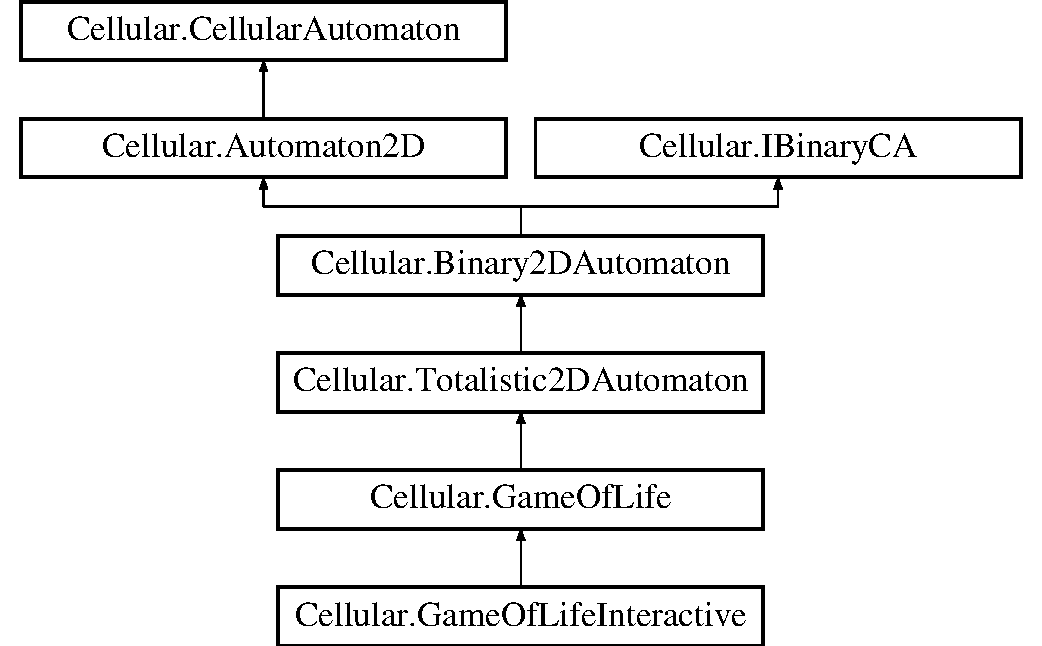
\includegraphics[height=5.000000cm]{class_cellular_1_1_binary2_d_automaton}
\end{center}
\end{figure}
\subsection*{Public Member Functions}
\begin{DoxyCompactItemize}
\item 
\hyperlink{class_cellular_1_1_binary2_d_automaton_a6956aa8cc05e4d00c116d8cc5e8528d4}{Binary2\+D\+Automaton} (int \hyperlink{class_cellular_1_1_automaton2_d_a1e9e5ec637c747a859c346839c90d174}{width}, int height)
\begin{DoxyCompactList}\small\item\em Creates a new {\ttfamily \hyperlink{class_cellular_1_1_binary2_d_automaton}{Binary2\+D\+Automaton}} of given size with one living cell in the middle, the rest is dead. \end{DoxyCompactList}\item 
\hyperlink{class_cellular_1_1_binary2_d_automaton_ab2bdc13f759e29b0efe84995c74e5006}{Binary2\+D\+Automaton} (Bit\+Array\mbox{[}$\,$\mbox{]} \hyperlink{all__1_8js_ae8b87ff4be2ae1dd5267342795263360}{initial\+State})
\begin{DoxyCompactList}\small\item\em Creates a new {\ttfamily \hyperlink{class_cellular_1_1_binary2_d_automaton}{Binary2\+D\+Automaton}} of given initial state. \end{DoxyCompactList}\item 
\hyperlink{class_cellular_1_1_binary2_d_automaton_a465d87aeab9f265595e942e46308f75f}{Binary2\+D\+Automaton} (int \hyperlink{class_cellular_1_1_automaton2_d_a1e9e5ec637c747a859c346839c90d174}{width}, int height, Random rnd)
\begin{DoxyCompactList}\small\item\em Creates a new {\ttfamily \hyperlink{class_cellular_1_1_binary2_d_automaton}{Binary2\+D\+Automaton}} of given size with a random initial state. \end{DoxyCompactList}\item 
override int \hyperlink{class_cellular_1_1_binary2_d_automaton_af0b06d58b66367dbeb712f2c4237ff54}{Get\+Hash\+Code} ()
\end{DoxyCompactItemize}
\subsection*{Protected Member Functions}
\begin{DoxyCompactItemize}
\item 
abstract \hyperlink{interface_cellular_1_1_i_binary_c_a}{I\+Binary\+C\+A} \hyperlink{class_cellular_1_1_binary2_d_automaton_ad2d31668c7b8f8e959575e03b995273f}{clone\+Template} (Bit\+Array\mbox{[}$\,$\mbox{]} new\+Instance\+State)
\end{DoxyCompactItemize}
\subsection*{Protected Attributes}
\begin{DoxyCompactItemize}
\item 
Bit\+Array\mbox{[}$\,$\mbox{]} \hyperlink{class_cellular_1_1_binary2_d_automaton_abac140afbe1d9263ef35aa596c181407}{state}
\end{DoxyCompactItemize}


\subsection{Detailed Description}
Class containing base-\/constructors for all binary 2\+D automata and implementation of the {\ttfamily \hyperlink{interface_cellular_1_1_i_binary_c_a}{I\+Binary\+C\+A}} interface. The state is kept in an array of {\ttfamily Bit\+Array}s reprezenting rows. 



Definition at line 11 of file Binary2\+D\+Automaton.\+cs.



\subsection{Constructor \& Destructor Documentation}
\hypertarget{class_cellular_1_1_binary2_d_automaton_a6956aa8cc05e4d00c116d8cc5e8528d4}{}\index{Cellular\+::\+Binary2\+D\+Automaton@{Cellular\+::\+Binary2\+D\+Automaton}!Binary2\+D\+Automaton@{Binary2\+D\+Automaton}}
\index{Binary2\+D\+Automaton@{Binary2\+D\+Automaton}!Cellular\+::\+Binary2\+D\+Automaton@{Cellular\+::\+Binary2\+D\+Automaton}}
\subsubsection[{Binary2\+D\+Automaton(int width, int height)}]{\setlength{\rightskip}{0pt plus 5cm}Cellular.\+Binary2\+D\+Automaton.\+Binary2\+D\+Automaton (
\begin{DoxyParamCaption}
\item[{int}]{width, }
\item[{int}]{height}
\end{DoxyParamCaption}
)}\label{class_cellular_1_1_binary2_d_automaton_a6956aa8cc05e4d00c116d8cc5e8528d4}


Creates a new {\ttfamily \hyperlink{class_cellular_1_1_binary2_d_automaton}{Binary2\+D\+Automaton}} of given size with one living cell in the middle, the rest is dead. 


\begin{DoxyParams}{Parameters}
{\em width} & The width of the new C\+A (length of rows).\\
\hline
{\em height} & The height of the new C\+A (number of rows).\\
\hline
\end{DoxyParams}


Definition at line 20 of file Binary2\+D\+Automaton.\+cs.

\hypertarget{class_cellular_1_1_binary2_d_automaton_ab2bdc13f759e29b0efe84995c74e5006}{}\index{Cellular\+::\+Binary2\+D\+Automaton@{Cellular\+::\+Binary2\+D\+Automaton}!Binary2\+D\+Automaton@{Binary2\+D\+Automaton}}
\index{Binary2\+D\+Automaton@{Binary2\+D\+Automaton}!Cellular\+::\+Binary2\+D\+Automaton@{Cellular\+::\+Binary2\+D\+Automaton}}
\subsubsection[{Binary2\+D\+Automaton(\+Bit\+Array[] initial\+State)}]{\setlength{\rightskip}{0pt plus 5cm}Cellular.\+Binary2\+D\+Automaton.\+Binary2\+D\+Automaton (
\begin{DoxyParamCaption}
\item[{Bit\+Array\mbox{[}$\,$\mbox{]}}]{initial\+State}
\end{DoxyParamCaption}
)}\label{class_cellular_1_1_binary2_d_automaton_ab2bdc13f759e29b0efe84995c74e5006}


Creates a new {\ttfamily \hyperlink{class_cellular_1_1_binary2_d_automaton}{Binary2\+D\+Automaton}} of given initial state. 


\begin{DoxyParams}{Parameters}
{\em initial\+State} & An array of {\ttfamily Bit\+Array}s describing the initial state of the C\+A. This also determines the size (width, height) of the new C\+A.\\
\hline
\end{DoxyParams}


Definition at line 37 of file Binary2\+D\+Automaton.\+cs.

\hypertarget{class_cellular_1_1_binary2_d_automaton_a465d87aeab9f265595e942e46308f75f}{}\index{Cellular\+::\+Binary2\+D\+Automaton@{Cellular\+::\+Binary2\+D\+Automaton}!Binary2\+D\+Automaton@{Binary2\+D\+Automaton}}
\index{Binary2\+D\+Automaton@{Binary2\+D\+Automaton}!Cellular\+::\+Binary2\+D\+Automaton@{Cellular\+::\+Binary2\+D\+Automaton}}
\subsubsection[{Binary2\+D\+Automaton(int width, int height, Random rnd)}]{\setlength{\rightskip}{0pt plus 5cm}Cellular.\+Binary2\+D\+Automaton.\+Binary2\+D\+Automaton (
\begin{DoxyParamCaption}
\item[{int}]{width, }
\item[{int}]{height, }
\item[{Random}]{rnd}
\end{DoxyParamCaption}
)}\label{class_cellular_1_1_binary2_d_automaton_a465d87aeab9f265595e942e46308f75f}


Creates a new {\ttfamily \hyperlink{class_cellular_1_1_binary2_d_automaton}{Binary2\+D\+Automaton}} of given size with a random initial state. 


\begin{DoxyParams}{Parameters}
{\em width} & The width of the new C\+A (length of rows).\\
\hline
{\em height} & The height of the new C\+A (number of rows).\\
\hline
{\em rnd} & Pseudo\+R\+N\+G instance that will be used to generate the original state.\\
\hline
\end{DoxyParams}


Definition at line 50 of file Binary2\+D\+Automaton.\+cs.



\subsection{Member Function Documentation}
\hypertarget{class_cellular_1_1_binary2_d_automaton_ad2d31668c7b8f8e959575e03b995273f}{}\index{Cellular\+::\+Binary2\+D\+Automaton@{Cellular\+::\+Binary2\+D\+Automaton}!clone\+Template@{clone\+Template}}
\index{clone\+Template@{clone\+Template}!Cellular\+::\+Binary2\+D\+Automaton@{Cellular\+::\+Binary2\+D\+Automaton}}
\subsubsection[{clone\+Template(\+Bit\+Array[] new\+Instance\+State)}]{\setlength{\rightskip}{0pt plus 5cm}abstract {\bf I\+Binary\+C\+A} Cellular.\+Binary2\+D\+Automaton.\+clone\+Template (
\begin{DoxyParamCaption}
\item[{Bit\+Array\mbox{[}$\,$\mbox{]}}]{new\+Instance\+State}
\end{DoxyParamCaption}
)\hspace{0.3cm}{\ttfamily [protected]}, {\ttfamily [pure virtual]}}\label{class_cellular_1_1_binary2_d_automaton_ad2d31668c7b8f8e959575e03b995273f}


Implemented in \hyperlink{class_cellular_1_1_totalistic2_d_automaton_ad5cc3f46a556aa1b1c99bdfa92f5ba1d}{Cellular.\+Totalistic2\+D\+Automaton}.

\hypertarget{class_cellular_1_1_binary2_d_automaton_af0b06d58b66367dbeb712f2c4237ff54}{}\index{Cellular\+::\+Binary2\+D\+Automaton@{Cellular\+::\+Binary2\+D\+Automaton}!Get\+Hash\+Code@{Get\+Hash\+Code}}
\index{Get\+Hash\+Code@{Get\+Hash\+Code}!Cellular\+::\+Binary2\+D\+Automaton@{Cellular\+::\+Binary2\+D\+Automaton}}
\subsubsection[{Get\+Hash\+Code()}]{\setlength{\rightskip}{0pt plus 5cm}override int Cellular.\+Binary2\+D\+Automaton.\+Get\+Hash\+Code (
\begin{DoxyParamCaption}
{}
\end{DoxyParamCaption}
)}\label{class_cellular_1_1_binary2_d_automaton_af0b06d58b66367dbeb712f2c4237ff54}


Definition at line 158 of file Binary2\+D\+Automaton.\+cs.



\subsection{Member Data Documentation}
\hypertarget{class_cellular_1_1_binary2_d_automaton_abac140afbe1d9263ef35aa596c181407}{}\index{Cellular\+::\+Binary2\+D\+Automaton@{Cellular\+::\+Binary2\+D\+Automaton}!state@{state}}
\index{state@{state}!Cellular\+::\+Binary2\+D\+Automaton@{Cellular\+::\+Binary2\+D\+Automaton}}
\subsubsection[{state}]{\setlength{\rightskip}{0pt plus 5cm}Bit\+Array \mbox{[}$\,$\mbox{]} Cellular.\+Binary2\+D\+Automaton.\+state\hspace{0.3cm}{\ttfamily [protected]}}\label{class_cellular_1_1_binary2_d_automaton_abac140afbe1d9263ef35aa596c181407}


Definition at line 13 of file Binary2\+D\+Automaton.\+cs.



The documentation for this class was generated from the following file\+:\begin{DoxyCompactItemize}
\item 
C\+:/\+Martin/\+M\+F\+F/\+\_\+baka/\+Martin\+Dvorak/\+Cellular/\hyperlink{_binary2_d_automaton_8cs}{Binary2\+D\+Automaton.\+cs}\end{DoxyCompactItemize}

\hypertarget{class_cellular_1_1_binary_range_automaton}{}\section{Cellular.\+Binary\+Range\+Automaton Class Reference}
\label{class_cellular_1_1_binary_range_automaton}\index{Cellular.\+Binary\+Range\+Automaton@{Cellular.\+Binary\+Range\+Automaton}}


Class representing any binary 1\+D automaton with symmetric scope. The automaton has firmly set borders. Referencing a cell beyond borders acts as referencing a dead cell.  


Inheritance diagram for Cellular.\+Binary\+Range\+Automaton\+:\begin{figure}[H]
\begin{center}
\leavevmode
\includegraphics[height=5.000000cm]{class_cellular_1_1_binary_range_automaton}
\end{center}
\end{figure}
\subsection*{Public Member Functions}
\begin{DoxyCompactItemize}
\item 
\hyperlink{class_cellular_1_1_binary_range_automaton_a3b165a9e98e516bf7e9bdb8bb2fe16a7}{Binary\+Range\+Automaton} (byte scope, bool\mbox{[}$\,$\mbox{]} \hyperlink{class_cellular_1_1_binary_range_automaton_a4dda99c3151599c8ef12d08d7472144c}{rule}, int \hyperlink{class_cellular_1_1_automaton1_d_a915129ccf0f1e7092844c99ce6a28e5b}{size})
\begin{DoxyCompactList}\small\item\em Creates a new C\+A of a general rule with 000...00100...000 as its initial state. \end{DoxyCompactList}\item 
\hyperlink{class_cellular_1_1_binary_range_automaton_a704950c30ff58c587c8a717f9f2c839b}{Binary\+Range\+Automaton} (byte scope, bool\mbox{[}$\,$\mbox{]} \hyperlink{class_cellular_1_1_binary_range_automaton_a4dda99c3151599c8ef12d08d7472144c}{rule}, Bit\+Array \hyperlink{all__1_8js_ae8b87ff4be2ae1dd5267342795263360}{initial\+State})
\begin{DoxyCompactList}\small\item\em Creates a new C\+A of a general rule with defined inital state. \end{DoxyCompactList}\item 
override void \hyperlink{class_cellular_1_1_binary_range_automaton_ade1f5b831b9676f04f835c33d245b9e2}{Step} ()
\begin{DoxyCompactList}\small\item\em Performs one step of the cellular automaton. Always calls \end{DoxyCompactList}\item 
override object \hyperlink{class_cellular_1_1_binary_range_automaton_a12f010562e04785e0a7efb113302687e}{Clone} ()
\begin{DoxyCompactList}\small\item\em Creates an appropriate copy of the C\+A. Its type and the specific rule are always preserved. However, the time (number of steps executed on the specific instance) is set back to 0. \end{DoxyCompactList}\item 
override string \hyperlink{class_cellular_1_1_binary_range_automaton_afad205eb4fea51efd63b063f96bfda5c}{Tell\+Type} ()
\begin{DoxyCompactList}\small\item\em Announces the runtime type of the C\+A including info about its rule. It serves for debugging purposes. \end{DoxyCompactList}\end{DoxyCompactItemize}
\subsection*{Protected Member Functions}
\begin{DoxyCompactItemize}
\item 
virtual bool \hyperlink{class_cellular_1_1_binary_range_automaton_a462f8b1d9b77966e14bb0160a4a06dca}{get\+Value\+At} (int index)
\begin{DoxyCompactList}\small\item\em This method simplifies boundary conditions. \end{DoxyCompactList}\item 
override \hyperlink{interface_cellular_1_1_i_binary_c_a}{I\+Binary\+C\+A} \hyperlink{class_cellular_1_1_binary_range_automaton_a75d9e1fc19f9bfc470e66b12aaf1abe8}{clone\+Template} (Bit\+Array new\+Instance\+State)
\end{DoxyCompactItemize}
\subsection*{Protected Attributes}
\begin{DoxyCompactItemize}
\item 
bool\mbox{[}$\,$\mbox{]} \hyperlink{class_cellular_1_1_binary_range_automaton_a4dda99c3151599c8ef12d08d7472144c}{rule}
\item 
byte \hyperlink{class_cellular_1_1_binary_range_automaton_a9a391c738dc7725aa66a52dca039a2f7}{range}
\end{DoxyCompactItemize}


\subsection{Detailed Description}
Class representing any binary 1\+D automaton with symmetric scope. The automaton has firmly set borders. Referencing a cell beyond borders acts as referencing a dead cell. 



Definition at line 10 of file Binary\+Range\+Automaton.\+cs.



\subsection{Constructor \& Destructor Documentation}
\hypertarget{class_cellular_1_1_binary_range_automaton_a3b165a9e98e516bf7e9bdb8bb2fe16a7}{}\index{Cellular\+::\+Binary\+Range\+Automaton@{Cellular\+::\+Binary\+Range\+Automaton}!Binary\+Range\+Automaton@{Binary\+Range\+Automaton}}
\index{Binary\+Range\+Automaton@{Binary\+Range\+Automaton}!Cellular\+::\+Binary\+Range\+Automaton@{Cellular\+::\+Binary\+Range\+Automaton}}
\subsubsection[{Binary\+Range\+Automaton(byte scope, bool[] rule, int size)}]{\setlength{\rightskip}{0pt plus 5cm}Cellular.\+Binary\+Range\+Automaton.\+Binary\+Range\+Automaton (
\begin{DoxyParamCaption}
\item[{byte}]{scope, }
\item[{bool\mbox{[}$\,$\mbox{]}}]{rule, }
\item[{int}]{size}
\end{DoxyParamCaption}
)}\label{class_cellular_1_1_binary_range_automaton_a3b165a9e98e516bf7e9bdb8bb2fe16a7}


Creates a new C\+A of a general rule with 000...00100...000 as its initial state. 


\begin{DoxyParams}{Parameters}
{\em scope} & How many cells on each side from the center determine the next state of the cell. Value 1 makes it equivalent to a {\ttfamily \hyperlink{class_cellular_1_1_elementary_automaton}{Elementary\+Automaton}} which has rule of size 8. Value 2 means that each new state of any cell depends on five total cells =$>$ size of rule must be 32.\\
\hline
{\em rule} & Array representing the rule for creating a new state. rule\mbox{[}0\mbox{]} is rule for 0..0, therefore opposite order to the rules of basic automata.\\
\hline
{\em size} & The size of the new C\+A.\\
\hline
\end{DoxyParams}


Definition at line 24 of file Binary\+Range\+Automaton.\+cs.

\hypertarget{class_cellular_1_1_binary_range_automaton_a704950c30ff58c587c8a717f9f2c839b}{}\index{Cellular\+::\+Binary\+Range\+Automaton@{Cellular\+::\+Binary\+Range\+Automaton}!Binary\+Range\+Automaton@{Binary\+Range\+Automaton}}
\index{Binary\+Range\+Automaton@{Binary\+Range\+Automaton}!Cellular\+::\+Binary\+Range\+Automaton@{Cellular\+::\+Binary\+Range\+Automaton}}
\subsubsection[{Binary\+Range\+Automaton(byte scope, bool[] rule, Bit\+Array initial\+State)}]{\setlength{\rightskip}{0pt plus 5cm}Cellular.\+Binary\+Range\+Automaton.\+Binary\+Range\+Automaton (
\begin{DoxyParamCaption}
\item[{byte}]{scope, }
\item[{bool\mbox{[}$\,$\mbox{]}}]{rule, }
\item[{Bit\+Array}]{initial\+State}
\end{DoxyParamCaption}
)}\label{class_cellular_1_1_binary_range_automaton_a704950c30ff58c587c8a717f9f2c839b}


Creates a new C\+A of a general rule with defined inital state. 


\begin{DoxyParams}{Parameters}
{\em scope} & How many cells on each side from the center determine the next state of the cell. Value 1 makes it equivalent to a {\ttfamily \hyperlink{class_cellular_1_1_elementary_automaton}{Elementary\+Automaton}} which has rule of size 8. Value 2 means that each new state of any cell depends on five total cells =$>$ size of rule must be 32.\\
\hline
{\em rule} & Array representing the rule for creating a new state. rule\mbox{[}0\mbox{]} is rule for 0..0, therefore opposite order to the rules of basic automata.\\
\hline
{\em initial\+State} & A {\ttfamily Bit\+Array} describing the initial state of the C\+A. This also determines the size of the new C\+A.\\
\hline
\end{DoxyParams}


Definition at line 39 of file Binary\+Range\+Automaton.\+cs.



\subsection{Member Function Documentation}
\hypertarget{class_cellular_1_1_binary_range_automaton_a12f010562e04785e0a7efb113302687e}{}\index{Cellular\+::\+Binary\+Range\+Automaton@{Cellular\+::\+Binary\+Range\+Automaton}!Clone@{Clone}}
\index{Clone@{Clone}!Cellular\+::\+Binary\+Range\+Automaton@{Cellular\+::\+Binary\+Range\+Automaton}}
\subsubsection[{Clone()}]{\setlength{\rightskip}{0pt plus 5cm}override object Cellular.\+Binary\+Range\+Automaton.\+Clone (
\begin{DoxyParamCaption}
{}
\end{DoxyParamCaption}
)\hspace{0.3cm}{\ttfamily [virtual]}}\label{class_cellular_1_1_binary_range_automaton_a12f010562e04785e0a7efb113302687e}


Creates an appropriate copy of the C\+A. Its type and the specific rule are always preserved. However, the time (number of steps executed on the specific instance) is set back to 0. 

\begin{DoxyReturn}{Returns}
A copy of the {\ttfamily \hyperlink{class_cellular_1_1_cellular_automaton}{Cellular\+Automaton}} as an {\ttfamily Object}
\end{DoxyReturn}


Implements \hyperlink{class_cellular_1_1_cellular_automaton_affd487b397cdbbbb1982815bbcd8e7d3}{Cellular.\+Cellular\+Automaton}.



Reimplemented in \hyperlink{class_cellular_1_1_binary_range_cyclic_automaton_a2361fe82802e372b24b8bec6a6135278}{Cellular.\+Binary\+Range\+Cyclic\+Automaton}.



Definition at line 105 of file Binary\+Range\+Automaton.\+cs.

\hypertarget{class_cellular_1_1_binary_range_automaton_a75d9e1fc19f9bfc470e66b12aaf1abe8}{}\index{Cellular\+::\+Binary\+Range\+Automaton@{Cellular\+::\+Binary\+Range\+Automaton}!clone\+Template@{clone\+Template}}
\index{clone\+Template@{clone\+Template}!Cellular\+::\+Binary\+Range\+Automaton@{Cellular\+::\+Binary\+Range\+Automaton}}
\subsubsection[{clone\+Template(\+Bit\+Array new\+Instance\+State)}]{\setlength{\rightskip}{0pt plus 5cm}override {\bf I\+Binary\+C\+A} Cellular.\+Binary\+Range\+Automaton.\+clone\+Template (
\begin{DoxyParamCaption}
\item[{Bit\+Array}]{new\+Instance\+State}
\end{DoxyParamCaption}
)\hspace{0.3cm}{\ttfamily [protected]}, {\ttfamily [virtual]}}\label{class_cellular_1_1_binary_range_automaton_a75d9e1fc19f9bfc470e66b12aaf1abe8}


Implements \hyperlink{class_cellular_1_1_binary1_d_automaton_a38ac5ae077c5d31356d278247fbab40a}{Cellular.\+Binary1\+D\+Automaton}.



Reimplemented in \hyperlink{class_cellular_1_1_binary_range_cyclic_automaton_a38ebc4d1f2610701299106475229c60b}{Cellular.\+Binary\+Range\+Cyclic\+Automaton}.



Definition at line 110 of file Binary\+Range\+Automaton.\+cs.

\hypertarget{class_cellular_1_1_binary_range_automaton_a462f8b1d9b77966e14bb0160a4a06dca}{}\index{Cellular\+::\+Binary\+Range\+Automaton@{Cellular\+::\+Binary\+Range\+Automaton}!get\+Value\+At@{get\+Value\+At}}
\index{get\+Value\+At@{get\+Value\+At}!Cellular\+::\+Binary\+Range\+Automaton@{Cellular\+::\+Binary\+Range\+Automaton}}
\subsubsection[{get\+Value\+At(int index)}]{\setlength{\rightskip}{0pt plus 5cm}virtual bool Cellular.\+Binary\+Range\+Automaton.\+get\+Value\+At (
\begin{DoxyParamCaption}
\item[{int}]{index}
\end{DoxyParamCaption}
)\hspace{0.3cm}{\ttfamily [protected]}, {\ttfamily [virtual]}}\label{class_cellular_1_1_binary_range_automaton_a462f8b1d9b77966e14bb0160a4a06dca}


This method simplifies boundary conditions. 


\begin{DoxyParams}{Parameters}
{\em index} & Zero-\/based index (which bit is required).\\
\hline
\end{DoxyParams}
\begin{DoxyReturn}{Returns}
One bit.
\end{DoxyReturn}


Reimplemented in \hyperlink{class_cellular_1_1_binary_range_cyclic_automaton_a0e4d7dd11fda253300ee9fc8adbc4d33}{Cellular.\+Binary\+Range\+Cyclic\+Automaton}.



Definition at line 62 of file Binary\+Range\+Automaton.\+cs.

\hypertarget{class_cellular_1_1_binary_range_automaton_ade1f5b831b9676f04f835c33d245b9e2}{}\index{Cellular\+::\+Binary\+Range\+Automaton@{Cellular\+::\+Binary\+Range\+Automaton}!Step@{Step}}
\index{Step@{Step}!Cellular\+::\+Binary\+Range\+Automaton@{Cellular\+::\+Binary\+Range\+Automaton}}
\subsubsection[{Step()}]{\setlength{\rightskip}{0pt plus 5cm}override void Cellular.\+Binary\+Range\+Automaton.\+Step (
\begin{DoxyParamCaption}
{}
\end{DoxyParamCaption}
)}\label{class_cellular_1_1_binary_range_automaton_ade1f5b831b9676f04f835c33d245b9e2}


Performs one step of the cellular automaton. Always calls 

{\ttfamily \hyperlink{class_cellular_1_1_cellular_automaton_aa70848d58015575974bc875ac5a89ae7}{Cellular\+Automaton.\+Step()};}. 

Implements \hyperlink{interface_cellular_1_1_i_binary_c_a_a6a04c7374538c49df07efa176e0dd3c3}{Cellular.\+I\+Binary\+C\+A}.



Definition at line 74 of file Binary\+Range\+Automaton.\+cs.

\hypertarget{class_cellular_1_1_binary_range_automaton_afad205eb4fea51efd63b063f96bfda5c}{}\index{Cellular\+::\+Binary\+Range\+Automaton@{Cellular\+::\+Binary\+Range\+Automaton}!Tell\+Type@{Tell\+Type}}
\index{Tell\+Type@{Tell\+Type}!Cellular\+::\+Binary\+Range\+Automaton@{Cellular\+::\+Binary\+Range\+Automaton}}
\subsubsection[{Tell\+Type()}]{\setlength{\rightskip}{0pt plus 5cm}override string Cellular.\+Binary\+Range\+Automaton.\+Tell\+Type (
\begin{DoxyParamCaption}
{}
\end{DoxyParamCaption}
)}\label{class_cellular_1_1_binary_range_automaton_afad205eb4fea51efd63b063f96bfda5c}


Announces the runtime type of the C\+A including info about its rule. It serves for debugging purposes. 

\begin{DoxyReturn}{Returns}
The same string as calling 
\begin{DoxyCode}
CellularAutomaton.TellType();
\end{DoxyCode}
.
\end{DoxyReturn}


Implements \hyperlink{interface_cellular_1_1_i_binary_c_a_aa67feabf5d1513aa74076d255c661948}{Cellular.\+I\+Binary\+C\+A}.



Definition at line 115 of file Binary\+Range\+Automaton.\+cs.



\subsection{Member Data Documentation}
\hypertarget{class_cellular_1_1_binary_range_automaton_a9a391c738dc7725aa66a52dca039a2f7}{}\index{Cellular\+::\+Binary\+Range\+Automaton@{Cellular\+::\+Binary\+Range\+Automaton}!range@{range}}
\index{range@{range}!Cellular\+::\+Binary\+Range\+Automaton@{Cellular\+::\+Binary\+Range\+Automaton}}
\subsubsection[{range}]{\setlength{\rightskip}{0pt plus 5cm}byte Cellular.\+Binary\+Range\+Automaton.\+range\hspace{0.3cm}{\ttfamily [protected]}}\label{class_cellular_1_1_binary_range_automaton_a9a391c738dc7725aa66a52dca039a2f7}


Definition at line 13 of file Binary\+Range\+Automaton.\+cs.

\hypertarget{class_cellular_1_1_binary_range_automaton_a4dda99c3151599c8ef12d08d7472144c}{}\index{Cellular\+::\+Binary\+Range\+Automaton@{Cellular\+::\+Binary\+Range\+Automaton}!rule@{rule}}
\index{rule@{rule}!Cellular\+::\+Binary\+Range\+Automaton@{Cellular\+::\+Binary\+Range\+Automaton}}
\subsubsection[{rule}]{\setlength{\rightskip}{0pt plus 5cm}bool \mbox{[}$\,$\mbox{]} Cellular.\+Binary\+Range\+Automaton.\+rule\hspace{0.3cm}{\ttfamily [protected]}}\label{class_cellular_1_1_binary_range_automaton_a4dda99c3151599c8ef12d08d7472144c}


Definition at line 12 of file Binary\+Range\+Automaton.\+cs.



The documentation for this class was generated from the following file\+:\begin{DoxyCompactItemize}
\item 
C\+:/\+Martin/\+M\+F\+F/\+\_\+baka/\+Martin\+Dvorak/\+Cellular/\hyperlink{_binary_range_automaton_8cs}{Binary\+Range\+Automaton.\+cs}\end{DoxyCompactItemize}

\hypertarget{class_cellular_1_1_binary_range_cyclic_automaton}{}\section{Cellular.\+Binary\+Range\+Cyclic\+Automaton Class Reference}
\label{class_cellular_1_1_binary_range_cyclic_automaton}\index{Cellular.\+Binary\+Range\+Cyclic\+Automaton@{Cellular.\+Binary\+Range\+Cyclic\+Automaton}}


Class representing any binary 1\+D automaton with symmetric scope. The automaton is cyclic -\/ its edges are connected. Therefore, all positions are equivalent.  


Inheritance diagram for Cellular.\+Binary\+Range\+Cyclic\+Automaton\+:\begin{figure}[H]
\begin{center}
\leavevmode
\includegraphics[height=5.000000cm]{class_cellular_1_1_binary_range_cyclic_automaton}
\end{center}
\end{figure}
\subsection*{Public Member Functions}
\begin{DoxyCompactItemize}
\item 
\hyperlink{class_cellular_1_1_binary_range_cyclic_automaton_a9f47b4027eba7db4a959946967ba371e}{Binary\+Range\+Cyclic\+Automaton} (byte scope, bool\mbox{[}$\,$\mbox{]} \hyperlink{class_cellular_1_1_binary_range_automaton_a4dda99c3151599c8ef12d08d7472144c}{rule}, int \hyperlink{class_cellular_1_1_automaton1_d_a915129ccf0f1e7092844c99ce6a28e5b}{size})
\begin{DoxyCompactList}\small\item\em Creates a new cyclic C\+A of a general rule with 000...00100...000 as its initial state. \end{DoxyCompactList}\item 
\hyperlink{class_cellular_1_1_binary_range_cyclic_automaton_a541a8c6eff23ec8afddc7388158df80e}{Binary\+Range\+Cyclic\+Automaton} (byte scope, bool\mbox{[}$\,$\mbox{]} \hyperlink{class_cellular_1_1_binary_range_automaton_a4dda99c3151599c8ef12d08d7472144c}{rule}, Bit\+Array \hyperlink{all__1_8js_ae8b87ff4be2ae1dd5267342795263360}{initial\+State})
\begin{DoxyCompactList}\small\item\em Creates a new cyclic C\+A of a general rule with defined inital state. \end{DoxyCompactList}\item 
override object \hyperlink{class_cellular_1_1_binary_range_cyclic_automaton_a2361fe82802e372b24b8bec6a6135278}{Clone} ()
\begin{DoxyCompactList}\small\item\em Creates an appropriate copy of the C\+A. Its type and the specific rule are always preserved. However, the time (number of steps executed on the specific instance) is set back to 0. \end{DoxyCompactList}\item 
override string \hyperlink{class_cellular_1_1_binary_range_cyclic_automaton_a75754d1c54550e1f29a9282647947cb8}{Tell\+Type} ()
\begin{DoxyCompactList}\small\item\em Announces the runtime type of the C\+A including info about its rule. It serves for debugging purposes. \end{DoxyCompactList}\item 
\hyperlink{class_cellular_1_1_reversible_automaton}{Reversible\+Automaton} \hyperlink{class_cellular_1_1_binary_range_cyclic_automaton_a68dc88c2cb78aaaf6246ebf6f058fbb9}{Convert\+To\+Reversible} (Bit\+Array previous\+State)
\end{DoxyCompactItemize}
\subsection*{Protected Member Functions}
\begin{DoxyCompactItemize}
\item 
override bool \hyperlink{class_cellular_1_1_binary_range_cyclic_automaton_a0e4d7dd11fda253300ee9fc8adbc4d33}{get\+Value\+At} (int index)
\begin{DoxyCompactList}\small\item\em This method simplifies boundary conditions. \end{DoxyCompactList}\item 
override \hyperlink{interface_cellular_1_1_i_binary_c_a}{I\+Binary\+C\+A} \hyperlink{class_cellular_1_1_binary_range_cyclic_automaton_a38ebc4d1f2610701299106475229c60b}{clone\+Template} (Bit\+Array new\+Instance\+State)
\end{DoxyCompactItemize}
\subsection*{Additional Inherited Members}


\subsection{Detailed Description}
Class representing any binary 1\+D automaton with symmetric scope. The automaton is cyclic -\/ its edges are connected. Therefore, all positions are equivalent. 



Definition at line 9 of file Binary\+Range\+Cyclic\+Automaton.\+cs.



\subsection{Constructor \& Destructor Documentation}
\hypertarget{class_cellular_1_1_binary_range_cyclic_automaton_a9f47b4027eba7db4a959946967ba371e}{}\index{Cellular\+::\+Binary\+Range\+Cyclic\+Automaton@{Cellular\+::\+Binary\+Range\+Cyclic\+Automaton}!Binary\+Range\+Cyclic\+Automaton@{Binary\+Range\+Cyclic\+Automaton}}
\index{Binary\+Range\+Cyclic\+Automaton@{Binary\+Range\+Cyclic\+Automaton}!Cellular\+::\+Binary\+Range\+Cyclic\+Automaton@{Cellular\+::\+Binary\+Range\+Cyclic\+Automaton}}
\subsubsection[{Binary\+Range\+Cyclic\+Automaton(byte scope, bool[] rule, int size)}]{\setlength{\rightskip}{0pt plus 5cm}Cellular.\+Binary\+Range\+Cyclic\+Automaton.\+Binary\+Range\+Cyclic\+Automaton (
\begin{DoxyParamCaption}
\item[{byte}]{scope, }
\item[{bool\mbox{[}$\,$\mbox{]}}]{rule, }
\item[{int}]{size}
\end{DoxyParamCaption}
)}\label{class_cellular_1_1_binary_range_cyclic_automaton_a9f47b4027eba7db4a959946967ba371e}


Creates a new cyclic C\+A of a general rule with 000...00100...000 as its initial state. 


\begin{DoxyParams}{Parameters}
{\em scope} & How many cells on each side from the center determine the next state of the cell. Value 1 makes it equivalent to a {\ttfamily \hyperlink{class_cellular_1_1_elementary_automaton}{Elementary\+Automaton}} which has rule of size 8. Value 2 means that each new state of any cell depends on five total cells =$>$ size of rule must be 32.\\
\hline
{\em rule} & Array representing the rule for creating a new state. rule\mbox{[}0\mbox{]} is rule for 0..0, therefore opposite order to the rules of basic automata.\\
\hline
{\em size} & The size of the new C\+A.\\
\hline
\end{DoxyParams}


Definition at line 20 of file Binary\+Range\+Cyclic\+Automaton.\+cs.

\hypertarget{class_cellular_1_1_binary_range_cyclic_automaton_a541a8c6eff23ec8afddc7388158df80e}{}\index{Cellular\+::\+Binary\+Range\+Cyclic\+Automaton@{Cellular\+::\+Binary\+Range\+Cyclic\+Automaton}!Binary\+Range\+Cyclic\+Automaton@{Binary\+Range\+Cyclic\+Automaton}}
\index{Binary\+Range\+Cyclic\+Automaton@{Binary\+Range\+Cyclic\+Automaton}!Cellular\+::\+Binary\+Range\+Cyclic\+Automaton@{Cellular\+::\+Binary\+Range\+Cyclic\+Automaton}}
\subsubsection[{Binary\+Range\+Cyclic\+Automaton(byte scope, bool[] rule, Bit\+Array initial\+State)}]{\setlength{\rightskip}{0pt plus 5cm}Cellular.\+Binary\+Range\+Cyclic\+Automaton.\+Binary\+Range\+Cyclic\+Automaton (
\begin{DoxyParamCaption}
\item[{byte}]{scope, }
\item[{bool\mbox{[}$\,$\mbox{]}}]{rule, }
\item[{Bit\+Array}]{initial\+State}
\end{DoxyParamCaption}
)}\label{class_cellular_1_1_binary_range_cyclic_automaton_a541a8c6eff23ec8afddc7388158df80e}


Creates a new cyclic C\+A of a general rule with defined inital state. 


\begin{DoxyParams}{Parameters}
{\em scope} & How many cells on each side from the center determine the next state of the cell. Value 1 makes it equivalent to a {\ttfamily \hyperlink{class_cellular_1_1_elementary_automaton}{Elementary\+Automaton}} which has rule of size 8. Value 2 means that each new state of any cell depends on five total cells =$>$ size of rule must be 32.\\
\hline
{\em rule} & Array representing the rule for creating a new state. rule\mbox{[}0\mbox{]} is rule for 0..0, therefore opposite order to the rules of basic automata.\\
\hline
{\em initial\+State} & A {\ttfamily Bit\+Array} describing the initial state of the C\+A. This also determines the size of the new C\+A.\\
\hline
\end{DoxyParams}


Definition at line 32 of file Binary\+Range\+Cyclic\+Automaton.\+cs.



\subsection{Member Function Documentation}
\hypertarget{class_cellular_1_1_binary_range_cyclic_automaton_a2361fe82802e372b24b8bec6a6135278}{}\index{Cellular\+::\+Binary\+Range\+Cyclic\+Automaton@{Cellular\+::\+Binary\+Range\+Cyclic\+Automaton}!Clone@{Clone}}
\index{Clone@{Clone}!Cellular\+::\+Binary\+Range\+Cyclic\+Automaton@{Cellular\+::\+Binary\+Range\+Cyclic\+Automaton}}
\subsubsection[{Clone()}]{\setlength{\rightskip}{0pt plus 5cm}override object Cellular.\+Binary\+Range\+Cyclic\+Automaton.\+Clone (
\begin{DoxyParamCaption}
{}
\end{DoxyParamCaption}
)\hspace{0.3cm}{\ttfamily [virtual]}}\label{class_cellular_1_1_binary_range_cyclic_automaton_a2361fe82802e372b24b8bec6a6135278}


Creates an appropriate copy of the C\+A. Its type and the specific rule are always preserved. However, the time (number of steps executed on the specific instance) is set back to 0. 

\begin{DoxyReturn}{Returns}
A copy of the {\ttfamily \hyperlink{class_cellular_1_1_cellular_automaton}{Cellular\+Automaton}} as an {\ttfamily Object}
\end{DoxyReturn}


Reimplemented from \hyperlink{class_cellular_1_1_binary_range_automaton_a12f010562e04785e0a7efb113302687e}{Cellular.\+Binary\+Range\+Automaton}.



Definition at line 46 of file Binary\+Range\+Cyclic\+Automaton.\+cs.

\hypertarget{class_cellular_1_1_binary_range_cyclic_automaton_a38ebc4d1f2610701299106475229c60b}{}\index{Cellular\+::\+Binary\+Range\+Cyclic\+Automaton@{Cellular\+::\+Binary\+Range\+Cyclic\+Automaton}!clone\+Template@{clone\+Template}}
\index{clone\+Template@{clone\+Template}!Cellular\+::\+Binary\+Range\+Cyclic\+Automaton@{Cellular\+::\+Binary\+Range\+Cyclic\+Automaton}}
\subsubsection[{clone\+Template(\+Bit\+Array new\+Instance\+State)}]{\setlength{\rightskip}{0pt plus 5cm}override {\bf I\+Binary\+C\+A} Cellular.\+Binary\+Range\+Cyclic\+Automaton.\+clone\+Template (
\begin{DoxyParamCaption}
\item[{Bit\+Array}]{new\+Instance\+State}
\end{DoxyParamCaption}
)\hspace{0.3cm}{\ttfamily [protected]}, {\ttfamily [virtual]}}\label{class_cellular_1_1_binary_range_cyclic_automaton_a38ebc4d1f2610701299106475229c60b}


Reimplemented from \hyperlink{class_cellular_1_1_binary_range_automaton_a75d9e1fc19f9bfc470e66b12aaf1abe8}{Cellular.\+Binary\+Range\+Automaton}.



Definition at line 51 of file Binary\+Range\+Cyclic\+Automaton.\+cs.

\hypertarget{class_cellular_1_1_binary_range_cyclic_automaton_a68dc88c2cb78aaaf6246ebf6f058fbb9}{}\index{Cellular\+::\+Binary\+Range\+Cyclic\+Automaton@{Cellular\+::\+Binary\+Range\+Cyclic\+Automaton}!Convert\+To\+Reversible@{Convert\+To\+Reversible}}
\index{Convert\+To\+Reversible@{Convert\+To\+Reversible}!Cellular\+::\+Binary\+Range\+Cyclic\+Automaton@{Cellular\+::\+Binary\+Range\+Cyclic\+Automaton}}
\subsubsection[{Convert\+To\+Reversible(\+Bit\+Array previous\+State)}]{\setlength{\rightskip}{0pt plus 5cm}{\bf Reversible\+Automaton} Cellular.\+Binary\+Range\+Cyclic\+Automaton.\+Convert\+To\+Reversible (
\begin{DoxyParamCaption}
\item[{Bit\+Array}]{previous\+State}
\end{DoxyParamCaption}
)}\label{class_cellular_1_1_binary_range_cyclic_automaton_a68dc88c2cb78aaaf6246ebf6f058fbb9}


Definition at line 61 of file Binary\+Range\+Cyclic\+Automaton.\+cs.

\hypertarget{class_cellular_1_1_binary_range_cyclic_automaton_a0e4d7dd11fda253300ee9fc8adbc4d33}{}\index{Cellular\+::\+Binary\+Range\+Cyclic\+Automaton@{Cellular\+::\+Binary\+Range\+Cyclic\+Automaton}!get\+Value\+At@{get\+Value\+At}}
\index{get\+Value\+At@{get\+Value\+At}!Cellular\+::\+Binary\+Range\+Cyclic\+Automaton@{Cellular\+::\+Binary\+Range\+Cyclic\+Automaton}}
\subsubsection[{get\+Value\+At(int index)}]{\setlength{\rightskip}{0pt plus 5cm}override bool Cellular.\+Binary\+Range\+Cyclic\+Automaton.\+get\+Value\+At (
\begin{DoxyParamCaption}
\item[{int}]{index}
\end{DoxyParamCaption}
)\hspace{0.3cm}{\ttfamily [protected]}, {\ttfamily [virtual]}}\label{class_cellular_1_1_binary_range_cyclic_automaton_a0e4d7dd11fda253300ee9fc8adbc4d33}


This method simplifies boundary conditions. 


\begin{DoxyParams}{Parameters}
{\em index} & Zero-\/based index (which bit is required).\\
\hline
\end{DoxyParams}
\begin{DoxyReturn}{Returns}
One bit.
\end{DoxyReturn}


Reimplemented from \hyperlink{class_cellular_1_1_binary_range_automaton_a462f8b1d9b77966e14bb0160a4a06dca}{Cellular.\+Binary\+Range\+Automaton}.



Definition at line 34 of file Binary\+Range\+Cyclic\+Automaton.\+cs.

\hypertarget{class_cellular_1_1_binary_range_cyclic_automaton_a75754d1c54550e1f29a9282647947cb8}{}\index{Cellular\+::\+Binary\+Range\+Cyclic\+Automaton@{Cellular\+::\+Binary\+Range\+Cyclic\+Automaton}!Tell\+Type@{Tell\+Type}}
\index{Tell\+Type@{Tell\+Type}!Cellular\+::\+Binary\+Range\+Cyclic\+Automaton@{Cellular\+::\+Binary\+Range\+Cyclic\+Automaton}}
\subsubsection[{Tell\+Type()}]{\setlength{\rightskip}{0pt plus 5cm}override string Cellular.\+Binary\+Range\+Cyclic\+Automaton.\+Tell\+Type (
\begin{DoxyParamCaption}
{}
\end{DoxyParamCaption}
)}\label{class_cellular_1_1_binary_range_cyclic_automaton_a75754d1c54550e1f29a9282647947cb8}


Announces the runtime type of the C\+A including info about its rule. It serves for debugging purposes. 

\begin{DoxyReturn}{Returns}
The same string as calling {\ttfamily \hyperlink{class_cellular_1_1_cellular_automaton_abe4b92fd405530c8a08cc07a3a19fff4}{Cellular\+Automaton.\+Tell\+Type()}}.
\end{DoxyReturn}


Implements \hyperlink{interface_cellular_1_1_i_binary_c_a_aa67feabf5d1513aa74076d255c661948}{Cellular.\+I\+Binary\+C\+A}.



Definition at line 56 of file Binary\+Range\+Cyclic\+Automaton.\+cs.



The documentation for this class was generated from the following file\+:\begin{DoxyCompactItemize}
\item 
C\+:/\+Martin/\+M\+F\+F/\+\_\+baka/\+Martin\+Dvorak/\+Cellular/\hyperlink{_binary_range_cyclic_automaton_8cs}{Binary\+Range\+Cyclic\+Automaton.\+cs}\end{DoxyCompactItemize}

\hypertarget{class_testing_1_1_binary_range_n_test}{}\section{Testing.\+Binary\+Range\+N\+Test Class Reference}
\label{class_testing_1_1_binary_range_n_test}\index{Testing.\+Binary\+Range\+N\+Test@{Testing.\+Binary\+Range\+N\+Test}}


Simple demonstration that {\ttfamily Binary\+Range\+Automaton} can be used in a place of {\ttfamily Elementary\+Automaton}.  


\subsection*{Static Public Member Functions}
\begin{DoxyCompactItemize}
\item 
static void \hyperlink{class_testing_1_1_binary_range_n_test_aa53181f8247ace374a9d9d291ba2170d}{Run\+Test} ()
\end{DoxyCompactItemize}


\subsection{Detailed Description}
Simple demonstration that {\ttfamily Binary\+Range\+Automaton} can be used in a place of {\ttfamily Elementary\+Automaton}. 



Definition at line 9 of file Binary\+Range\+N\+Test.\+cs.



\subsection{Member Function Documentation}
\hypertarget{class_testing_1_1_binary_range_n_test_aa53181f8247ace374a9d9d291ba2170d}{}\index{Testing\+::\+Binary\+Range\+N\+Test@{Testing\+::\+Binary\+Range\+N\+Test}!Run\+Test@{Run\+Test}}
\index{Run\+Test@{Run\+Test}!Testing\+::\+Binary\+Range\+N\+Test@{Testing\+::\+Binary\+Range\+N\+Test}}
\subsubsection[{Run\+Test()}]{\setlength{\rightskip}{0pt plus 5cm}static void Testing.\+Binary\+Range\+N\+Test.\+Run\+Test (
\begin{DoxyParamCaption}
{}
\end{DoxyParamCaption}
)\hspace{0.3cm}{\ttfamily [static]}}\label{class_testing_1_1_binary_range_n_test_aa53181f8247ace374a9d9d291ba2170d}


Definition at line 11 of file Binary\+Range\+N\+Test.\+cs.



The documentation for this class was generated from the following file\+:\begin{DoxyCompactItemize}
\item 
C\+:/\+Martin/\+M\+F\+F/\+\_\+baka/\+Martin\+Dvorak/\+Testing/\hyperlink{_binary_range_n_test_8cs}{Binary\+Range\+N\+Test.\+cs}\end{DoxyCompactItemize}

\hypertarget{class_crypto_1_1_cannot_generate_exception}{}\section{Crypto.\+Cannot\+Generate\+Exception Class Reference}
\label{class_crypto_1_1_cannot_generate_exception}\index{Crypto.\+Cannot\+Generate\+Exception@{Crypto.\+Cannot\+Generate\+Exception}}


Custom exception that any key extender can throw.  


Inheritance diagram for Crypto.\+Cannot\+Generate\+Exception\+:\begin{figure}[H]
\begin{center}
\leavevmode
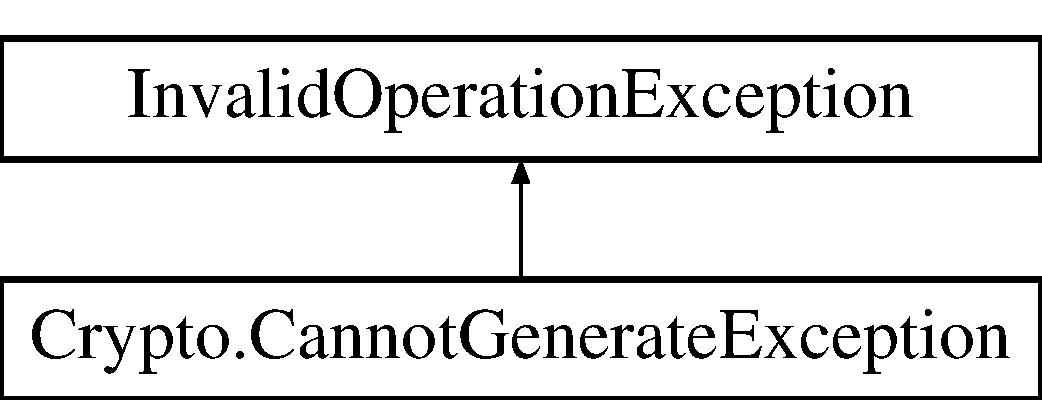
\includegraphics[height=2.000000cm]{class_crypto_1_1_cannot_generate_exception}
\end{center}
\end{figure}
\subsection*{Public Member Functions}
\begin{DoxyCompactItemize}
\item 
\hyperlink{class_crypto_1_1_cannot_generate_exception_a17a4ab8ac6a435318f69bf88ae224598}{Cannot\+Generate\+Exception} ()
\item 
\hyperlink{class_crypto_1_1_cannot_generate_exception_acc186360edfaaa431c4c64ef7562dd56}{Cannot\+Generate\+Exception} (string message)
\item 
\hyperlink{class_crypto_1_1_cannot_generate_exception_a85fc7abc1f61642c128e1d14d2985ecf}{Cannot\+Generate\+Exception} (string message, Exception inner\+Exception)
\end{DoxyCompactItemize}


\subsection{Detailed Description}
Custom exception that any key extender can throw. 



Definition at line 8 of file Cannot\+Generate\+Exception.\+cs.



\subsection{Constructor \& Destructor Documentation}
\hypertarget{class_crypto_1_1_cannot_generate_exception_a17a4ab8ac6a435318f69bf88ae224598}{}\index{Crypto\+::\+Cannot\+Generate\+Exception@{Crypto\+::\+Cannot\+Generate\+Exception}!Cannot\+Generate\+Exception@{Cannot\+Generate\+Exception}}
\index{Cannot\+Generate\+Exception@{Cannot\+Generate\+Exception}!Crypto\+::\+Cannot\+Generate\+Exception@{Crypto\+::\+Cannot\+Generate\+Exception}}
\subsubsection[{Cannot\+Generate\+Exception()}]{\setlength{\rightskip}{0pt plus 5cm}Crypto.\+Cannot\+Generate\+Exception.\+Cannot\+Generate\+Exception (
\begin{DoxyParamCaption}
{}
\end{DoxyParamCaption}
)}\label{class_crypto_1_1_cannot_generate_exception_a17a4ab8ac6a435318f69bf88ae224598}


Definition at line 10 of file Cannot\+Generate\+Exception.\+cs.

\hypertarget{class_crypto_1_1_cannot_generate_exception_acc186360edfaaa431c4c64ef7562dd56}{}\index{Crypto\+::\+Cannot\+Generate\+Exception@{Crypto\+::\+Cannot\+Generate\+Exception}!Cannot\+Generate\+Exception@{Cannot\+Generate\+Exception}}
\index{Cannot\+Generate\+Exception@{Cannot\+Generate\+Exception}!Crypto\+::\+Cannot\+Generate\+Exception@{Crypto\+::\+Cannot\+Generate\+Exception}}
\subsubsection[{Cannot\+Generate\+Exception(string message)}]{\setlength{\rightskip}{0pt plus 5cm}Crypto.\+Cannot\+Generate\+Exception.\+Cannot\+Generate\+Exception (
\begin{DoxyParamCaption}
\item[{string}]{message}
\end{DoxyParamCaption}
)}\label{class_crypto_1_1_cannot_generate_exception_acc186360edfaaa431c4c64ef7562dd56}


Definition at line 11 of file Cannot\+Generate\+Exception.\+cs.

\hypertarget{class_crypto_1_1_cannot_generate_exception_a85fc7abc1f61642c128e1d14d2985ecf}{}\index{Crypto\+::\+Cannot\+Generate\+Exception@{Crypto\+::\+Cannot\+Generate\+Exception}!Cannot\+Generate\+Exception@{Cannot\+Generate\+Exception}}
\index{Cannot\+Generate\+Exception@{Cannot\+Generate\+Exception}!Crypto\+::\+Cannot\+Generate\+Exception@{Crypto\+::\+Cannot\+Generate\+Exception}}
\subsubsection[{Cannot\+Generate\+Exception(string message, Exception inner\+Exception)}]{\setlength{\rightskip}{0pt plus 5cm}Crypto.\+Cannot\+Generate\+Exception.\+Cannot\+Generate\+Exception (
\begin{DoxyParamCaption}
\item[{string}]{message, }
\item[{Exception}]{inner\+Exception}
\end{DoxyParamCaption}
)}\label{class_crypto_1_1_cannot_generate_exception_a85fc7abc1f61642c128e1d14d2985ecf}


Definition at line 12 of file Cannot\+Generate\+Exception.\+cs.



The documentation for this class was generated from the following file\+:\begin{DoxyCompactItemize}
\item 
C\+:/\+Martin/\+M\+F\+F/\+\_\+baka/\+Martin\+Dvorak/\+Crypto/\hyperlink{_cannot_generate_exception_8cs}{Cannot\+Generate\+Exception.\+cs}\end{DoxyCompactItemize}

\hypertarget{class_cellular_1_1_cellular_automaton}{}\section{Cellular.\+Cellular\+Automaton Class Reference}
\label{class_cellular_1_1_cellular_automaton}\index{Cellular.\+Cellular\+Automaton@{Cellular.\+Cellular\+Automaton}}


The top class of the C\+A hierarchy. Every constructor should follow this logical order when considering its parametres\+: specification of the type (usually not needed), rule, size, initial state / rng.  


Inheritance diagram for Cellular.\+Cellular\+Automaton\+:\begin{figure}[H]
\begin{center}
\leavevmode
\includegraphics[height=2.788845cm]{class_cellular_1_1_cellular_automaton}
\end{center}
\end{figure}
\subsection*{Public Member Functions}
\begin{DoxyCompactItemize}
\item 
abstract void \hyperlink{class_cellular_1_1_cellular_automaton_aa70848d58015575974bc875ac5a89ae7}{Step} ()
\begin{DoxyCompactList}\small\item\em Performs one step applying the specific rule for creating a new state. \end{DoxyCompactList}\item 
uint \hyperlink{class_cellular_1_1_cellular_automaton_a340d1faea1300db9183b4b4368d4f838}{Get\+Time} ()
\begin{DoxyCompactList}\small\item\em Only returns how many steps have been done. \end{DoxyCompactList}\item 
void \hyperlink{class_cellular_1_1_cellular_automaton_ad4948be8db73c5e052e2c5e59ac85ad8}{Step} (uint times)
\begin{DoxyCompactList}\small\item\em Performs the step n times. \end{DoxyCompactList}\item 
abstract object \hyperlink{class_cellular_1_1_cellular_automaton_affd487b397cdbbbb1982815bbcd8e7d3}{Clone} ()
\begin{DoxyCompactList}\small\item\em Creates an appropriate copy of the C\+A. Its type and the specific rule are always preserved. However, the time (number of steps executed on the specific instance) is set back to 0. \end{DoxyCompactList}\item 
abstract string \hyperlink{class_cellular_1_1_cellular_automaton_abe4b92fd405530c8a08cc07a3a19fff4}{Tell\+Type} ()
\begin{DoxyCompactList}\small\item\em Announces the runtime type of the C\+A including info about its rule. It serves for debugging purposes. \end{DoxyCompactList}\end{DoxyCompactItemize}
\subsection*{Protected Attributes}
\begin{DoxyCompactItemize}
\item 
uint \hyperlink{class_cellular_1_1_cellular_automaton_a6eaa8a9840fbc4c875d4e7d5a14e5f70}{time} = 0
\end{DoxyCompactItemize}


\subsection{Detailed Description}
The top class of the C\+A hierarchy. Every constructor should follow this logical order when considering its parametres\+: specification of the type (usually not needed), rule, size, initial state / rng. 



Definition at line 7 of file Cellular\+Automaton.\+cs.



\subsection{Member Function Documentation}
\hypertarget{class_cellular_1_1_cellular_automaton_affd487b397cdbbbb1982815bbcd8e7d3}{}\index{Cellular\+::\+Cellular\+Automaton@{Cellular\+::\+Cellular\+Automaton}!Clone@{Clone}}
\index{Clone@{Clone}!Cellular\+::\+Cellular\+Automaton@{Cellular\+::\+Cellular\+Automaton}}
\subsubsection[{Clone()}]{\setlength{\rightskip}{0pt plus 5cm}abstract object Cellular.\+Cellular\+Automaton.\+Clone (
\begin{DoxyParamCaption}
{}
\end{DoxyParamCaption}
)\hspace{0.3cm}{\ttfamily [pure virtual]}}\label{class_cellular_1_1_cellular_automaton_affd487b397cdbbbb1982815bbcd8e7d3}


Creates an appropriate copy of the C\+A. Its type and the specific rule are always preserved. However, the time (number of steps executed on the specific instance) is set back to 0. 

\begin{DoxyReturn}{Returns}
A copy of the {\ttfamily \hyperlink{class_cellular_1_1_cellular_automaton}{Cellular\+Automaton}} as an {\ttfamily Object}
\end{DoxyReturn}


Implemented in \hyperlink{class_cellular_1_1_totalistic2_d_automaton_ae78cf4c3f8245adf64ec9a173330804f}{Cellular.\+Totalistic2\+D\+Automaton}, \hyperlink{class_cellular_1_1_elementary_fast_automaton_a98bbdcade0ac93dd0fbc96ba253c2978}{Cellular.\+Elementary\+Fast\+Automaton}, \hyperlink{class_cellular_1_1_binary_range_automaton_a12f010562e04785e0a7efb113302687e}{Cellular.\+Binary\+Range\+Automaton}, \hyperlink{class_cellular_1_1_elementary_automaton_ada4ddee98167e8f4f4b6dea1f7563b47}{Cellular.\+Elementary\+Automaton}, \hyperlink{class_cellular_1_1_binary_range_cyclic_automaton_a2361fe82802e372b24b8bec6a6135278}{Cellular.\+Binary\+Range\+Cyclic\+Automaton}, \hyperlink{class_cellular_1_1_nary_totalistic_automaton_a13f16113915ecec451fc4764a32044f9}{Cellular.\+Nary\+Totalistic\+Automaton}, and \hyperlink{class_cellular_1_1_nary_totalistic_cyclic_automaton_aa8d5a7d77a6dfc5f6e4fae6ba1c6cfd0}{Cellular.\+Nary\+Totalistic\+Cyclic\+Automaton}.

\hypertarget{class_cellular_1_1_cellular_automaton_a340d1faea1300db9183b4b4368d4f838}{}\index{Cellular\+::\+Cellular\+Automaton@{Cellular\+::\+Cellular\+Automaton}!Get\+Time@{Get\+Time}}
\index{Get\+Time@{Get\+Time}!Cellular\+::\+Cellular\+Automaton@{Cellular\+::\+Cellular\+Automaton}}
\subsubsection[{Get\+Time()}]{\setlength{\rightskip}{0pt plus 5cm}uint Cellular.\+Cellular\+Automaton.\+Get\+Time (
\begin{DoxyParamCaption}
{}
\end{DoxyParamCaption}
)}\label{class_cellular_1_1_cellular_automaton_a340d1faea1300db9183b4b4368d4f838}


Only returns how many steps have been done. 

\begin{DoxyReturn}{Returns}
Number of executed steps.
\end{DoxyReturn}


Definition at line 20 of file Cellular\+Automaton.\+cs.

\hypertarget{class_cellular_1_1_cellular_automaton_aa70848d58015575974bc875ac5a89ae7}{}\index{Cellular\+::\+Cellular\+Automaton@{Cellular\+::\+Cellular\+Automaton}!Step@{Step}}
\index{Step@{Step}!Cellular\+::\+Cellular\+Automaton@{Cellular\+::\+Cellular\+Automaton}}
\subsubsection[{Step()}]{\setlength{\rightskip}{0pt plus 5cm}abstract void Cellular.\+Cellular\+Automaton.\+Step (
\begin{DoxyParamCaption}
{}
\end{DoxyParamCaption}
)\hspace{0.3cm}{\ttfamily [pure virtual]}}\label{class_cellular_1_1_cellular_automaton_aa70848d58015575974bc875ac5a89ae7}


Performs one step applying the specific rule for creating a new state. 



Implemented in \hyperlink{class_cellular_1_1_totalistic2_d_automaton_a7f85cac5420f67a936cbd4cef33c4abc}{Cellular.\+Totalistic2\+D\+Automaton}, \hyperlink{class_cellular_1_1_elementary_automaton_adae7c322e4c7cd00cd0534a23d1abfa4}{Cellular.\+Elementary\+Automaton}, \hyperlink{class_cellular_1_1_binary_range_automaton_ade1f5b831b9676f04f835c33d245b9e2}{Cellular.\+Binary\+Range\+Automaton}, \hyperlink{class_cellular_1_1_elementary_fast_automaton_aa877bef8b8242c58e190a884d18f3b5f}{Cellular.\+Elementary\+Fast\+Automaton}, and \hyperlink{class_cellular_1_1_nary_totalistic_automaton_ad90769a438ab94b46d4750a571782056}{Cellular.\+Nary\+Totalistic\+Automaton}.

\hypertarget{class_cellular_1_1_cellular_automaton_ad4948be8db73c5e052e2c5e59ac85ad8}{}\index{Cellular\+::\+Cellular\+Automaton@{Cellular\+::\+Cellular\+Automaton}!Step@{Step}}
\index{Step@{Step}!Cellular\+::\+Cellular\+Automaton@{Cellular\+::\+Cellular\+Automaton}}
\subsubsection[{Step(uint times)}]{\setlength{\rightskip}{0pt plus 5cm}void Cellular.\+Cellular\+Automaton.\+Step (
\begin{DoxyParamCaption}
\item[{uint}]{times}
\end{DoxyParamCaption}
)}\label{class_cellular_1_1_cellular_automaton_ad4948be8db73c5e052e2c5e59ac85ad8}


Performs the step n times. 


\begin{DoxyParams}{Parameters}
{\em times} & How many times {\ttfamily \hyperlink{class_cellular_1_1_cellular_automaton_aa70848d58015575974bc875ac5a89ae7}{Step()}} should be called.\\
\hline
\end{DoxyParams}


Definition at line 29 of file Cellular\+Automaton.\+cs.

\hypertarget{class_cellular_1_1_cellular_automaton_abe4b92fd405530c8a08cc07a3a19fff4}{}\index{Cellular\+::\+Cellular\+Automaton@{Cellular\+::\+Cellular\+Automaton}!Tell\+Type@{Tell\+Type}}
\index{Tell\+Type@{Tell\+Type}!Cellular\+::\+Cellular\+Automaton@{Cellular\+::\+Cellular\+Automaton}}
\subsubsection[{Tell\+Type()}]{\setlength{\rightskip}{0pt plus 5cm}abstract string Cellular.\+Cellular\+Automaton.\+Tell\+Type (
\begin{DoxyParamCaption}
{}
\end{DoxyParamCaption}
)\hspace{0.3cm}{\ttfamily [pure virtual]}}\label{class_cellular_1_1_cellular_automaton_abe4b92fd405530c8a08cc07a3a19fff4}


Announces the runtime type of the C\+A including info about its rule. It serves for debugging purposes. 

\begin{DoxyReturn}{Returns}
Type of the C\+A as a string.
\end{DoxyReturn}


Implemented in \hyperlink{class_cellular_1_1_totalistic2_d_automaton_aa009c674cd109fa70173e9893f6d3b09}{Cellular.\+Totalistic2\+D\+Automaton}, \hyperlink{class_cellular_1_1_binary_range_automaton_afad205eb4fea51efd63b063f96bfda5c}{Cellular.\+Binary\+Range\+Automaton}, \hyperlink{class_cellular_1_1_elementary_automaton_a812677139d560e2c600226361b785995}{Cellular.\+Elementary\+Automaton}, \hyperlink{class_cellular_1_1_binary_range_cyclic_automaton_a75754d1c54550e1f29a9282647947cb8}{Cellular.\+Binary\+Range\+Cyclic\+Automaton}, \hyperlink{class_cellular_1_1_nary_totalistic_automaton_aa691c532a55638c7e3d0c125a4244773}{Cellular.\+Nary\+Totalistic\+Automaton}, and \hyperlink{class_cellular_1_1_nary_totalistic_cyclic_automaton_ac5c39cfb72386e3ab6132ab420091ae9}{Cellular.\+Nary\+Totalistic\+Cyclic\+Automaton}.



\subsection{Member Data Documentation}
\hypertarget{class_cellular_1_1_cellular_automaton_a6eaa8a9840fbc4c875d4e7d5a14e5f70}{}\index{Cellular\+::\+Cellular\+Automaton@{Cellular\+::\+Cellular\+Automaton}!time@{time}}
\index{time@{time}!Cellular\+::\+Cellular\+Automaton@{Cellular\+::\+Cellular\+Automaton}}
\subsubsection[{time}]{\setlength{\rightskip}{0pt plus 5cm}uint Cellular.\+Cellular\+Automaton.\+time = 0\hspace{0.3cm}{\ttfamily [protected]}}\label{class_cellular_1_1_cellular_automaton_a6eaa8a9840fbc4c875d4e7d5a14e5f70}


Definition at line 9 of file Cellular\+Automaton.\+cs.



The documentation for this class was generated from the following file\+:\begin{DoxyCompactItemize}
\item 
C\+:/\+Martin/\+M\+F\+F/\+\_\+baka/\+Martin\+Dvorak/\+Cellular/\hyperlink{_cellular_automaton_8cs}{Cellular\+Automaton.\+cs}\end{DoxyCompactItemize}

\hypertarget{class_program_1_1_crypto_form}{}\section{Program.\+Crypto\+Form Class Reference}
\label{class_program_1_1_crypto_form}\index{Program.\+Crypto\+Form@{Program.\+Crypto\+Form}}


Windows application for users who want to encrypt their data using a cellular automata based algorithm.  


Inheritance diagram for Program.\+Crypto\+Form\+:\begin{figure}[H]
\begin{center}
\leavevmode
\includegraphics[height=2.000000cm]{class_program_1_1_crypto_form}
\end{center}
\end{figure}
\subsection*{Public Member Functions}
\begin{DoxyCompactItemize}
\item 
\hyperlink{class_program_1_1_crypto_form_ab4de171d2fe2499055864e45f9efa4cc}{Crypto\+Form} ()
\end{DoxyCompactItemize}
\subsection*{Protected Member Functions}
\begin{DoxyCompactItemize}
\item 
override void \hyperlink{class_program_1_1_crypto_form_adaa80d92f4324b9d835d8125dcda4582}{Dispose} (bool disposing)
\begin{DoxyCompactList}\small\item\em Clean up any resources being used. \end{DoxyCompactList}\end{DoxyCompactItemize}


\subsection{Detailed Description}
Windows application for users who want to encrypt their data using a cellular automata based algorithm. 



Definition at line 11 of file Crypto\+Form.\+cs.



\subsection{Constructor \& Destructor Documentation}
\hypertarget{class_program_1_1_crypto_form_ab4de171d2fe2499055864e45f9efa4cc}{}\index{Program\+::\+Crypto\+Form@{Program\+::\+Crypto\+Form}!Crypto\+Form@{Crypto\+Form}}
\index{Crypto\+Form@{Crypto\+Form}!Program\+::\+Crypto\+Form@{Program\+::\+Crypto\+Form}}
\subsubsection[{Crypto\+Form()}]{\setlength{\rightskip}{0pt plus 5cm}Program.\+Crypto\+Form.\+Crypto\+Form (
\begin{DoxyParamCaption}
{}
\end{DoxyParamCaption}
)}\label{class_program_1_1_crypto_form_ab4de171d2fe2499055864e45f9efa4cc}


Definition at line 15 of file Crypto\+Form.\+cs.



\subsection{Member Function Documentation}
\hypertarget{class_program_1_1_crypto_form_adaa80d92f4324b9d835d8125dcda4582}{}\index{Program\+::\+Crypto\+Form@{Program\+::\+Crypto\+Form}!Dispose@{Dispose}}
\index{Dispose@{Dispose}!Program\+::\+Crypto\+Form@{Program\+::\+Crypto\+Form}}
\subsubsection[{Dispose(bool disposing)}]{\setlength{\rightskip}{0pt plus 5cm}override void Program.\+Crypto\+Form.\+Dispose (
\begin{DoxyParamCaption}
\item[{bool}]{disposing}
\end{DoxyParamCaption}
)\hspace{0.3cm}{\ttfamily [protected]}}\label{class_program_1_1_crypto_form_adaa80d92f4324b9d835d8125dcda4582}


Clean up any resources being used. 


\begin{DoxyParams}{Parameters}
{\em disposing} & true if managed resources should be disposed; otherwise, false.\\
\hline
\end{DoxyParams}


Definition at line 14 of file Crypto\+Form.\+Designer.\+cs.



The documentation for this class was generated from the following files\+:\begin{DoxyCompactItemize}
\item 
C\+:/\+Martin/\+M\+F\+F/\+\_\+baka/\+Program/\hyperlink{_crypto_form_8cs}{Crypto\+Form.\+cs}\item 
C\+:/\+Martin/\+M\+F\+F/\+\_\+baka/\+Program/\hyperlink{_crypto_form_8_designer_8cs}{Crypto\+Form.\+Designer.\+cs}\end{DoxyCompactItemize}

\hypertarget{class_user_forms_1_1_demo_form}{}\section{User\+Forms.\+Demo\+Form Class Reference}
\label{class_user_forms_1_1_demo_form}\index{User\+Forms.\+Demo\+Form@{User\+Forms.\+Demo\+Form}}


Interactive visual demo of the Game of Life on a rectangular playground. This is not a platform for programming or serious experiments.  


Inheritance diagram for User\+Forms.\+Demo\+Form\+:\begin{figure}[H]
\begin{center}
\leavevmode
\includegraphics[height=2.000000cm]{class_user_forms_1_1_demo_form}
\end{center}
\end{figure}
\subsection*{Public Member Functions}
\begin{DoxyCompactItemize}
\item 
\hyperlink{class_user_forms_1_1_demo_form_a9ef677039850f5ac014ad27d1aa95160}{Demo\+Form} ()
\end{DoxyCompactItemize}
\subsection*{Protected Member Functions}
\begin{DoxyCompactItemize}
\item 
override void \hyperlink{class_user_forms_1_1_demo_form_a1dd0d43c1b10b64a4591d4b6235f0148}{Dispose} (bool disposing)
\begin{DoxyCompactList}\small\item\em Clean up any resources being used. \end{DoxyCompactList}\end{DoxyCompactItemize}


\subsection{Detailed Description}
Interactive visual demo of the Game of Life on a rectangular playground. This is not a platform for programming or serious experiments. 



Definition at line 14 of file Demo\+Form.\+cs.



\subsection{Constructor \& Destructor Documentation}
\hypertarget{class_user_forms_1_1_demo_form_a9ef677039850f5ac014ad27d1aa95160}{}\index{User\+Forms\+::\+Demo\+Form@{User\+Forms\+::\+Demo\+Form}!Demo\+Form@{Demo\+Form}}
\index{Demo\+Form@{Demo\+Form}!User\+Forms\+::\+Demo\+Form@{User\+Forms\+::\+Demo\+Form}}
\subsubsection[{Demo\+Form()}]{\setlength{\rightskip}{0pt plus 5cm}User\+Forms.\+Demo\+Form.\+Demo\+Form (
\begin{DoxyParamCaption}
{}
\end{DoxyParamCaption}
)}\label{class_user_forms_1_1_demo_form_a9ef677039850f5ac014ad27d1aa95160}


Definition at line 23 of file Demo\+Form.\+cs.



\subsection{Member Function Documentation}
\hypertarget{class_user_forms_1_1_demo_form_a1dd0d43c1b10b64a4591d4b6235f0148}{}\index{User\+Forms\+::\+Demo\+Form@{User\+Forms\+::\+Demo\+Form}!Dispose@{Dispose}}
\index{Dispose@{Dispose}!User\+Forms\+::\+Demo\+Form@{User\+Forms\+::\+Demo\+Form}}
\subsubsection[{Dispose(bool disposing)}]{\setlength{\rightskip}{0pt plus 5cm}override void User\+Forms.\+Demo\+Form.\+Dispose (
\begin{DoxyParamCaption}
\item[{bool}]{disposing}
\end{DoxyParamCaption}
)\hspace{0.3cm}{\ttfamily [protected]}}\label{class_user_forms_1_1_demo_form_a1dd0d43c1b10b64a4591d4b6235f0148}


Clean up any resources being used. 


\begin{DoxyParams}{Parameters}
{\em disposing} & true if managed resources should be disposed; otherwise, false.\\
\hline
\end{DoxyParams}


Definition at line 14 of file Demo\+Form.\+Designer.\+cs.



The documentation for this class was generated from the following files\+:\begin{DoxyCompactItemize}
\item 
C\+:/\+Martin/\+M\+F\+F/\+\_\+baka/\+Martin\+Dvorak/\+User\+Forms/\hyperlink{_demo_form_8cs}{Demo\+Form.\+cs}\item 
C\+:/\+Martin/\+M\+F\+F/\+\_\+baka/\+Martin\+Dvorak/\+User\+Forms/\hyperlink{_demo_form_8_designer_8cs}{Demo\+Form.\+Designer.\+cs}\end{DoxyCompactItemize}

\hypertarget{class_cellular_1_1_elementary_automaton}{}\section{Cellular.\+Elementary\+Automaton Class Reference}
\label{class_cellular_1_1_elementary_automaton}\index{Cellular.\+Elementary\+Automaton@{Cellular.\+Elementary\+Automaton}}


Class representing 256 elementary C\+A with firmly set borders. This specific implementation calculates every bit separately.  


Inheritance diagram for Cellular.\+Elementary\+Automaton\+:\begin{figure}[H]
\begin{center}
\leavevmode
\includegraphics[height=5.000000cm]{class_cellular_1_1_elementary_automaton}
\end{center}
\end{figure}
\subsection*{Public Member Functions}
\begin{DoxyCompactItemize}
\item 
\hyperlink{class_cellular_1_1_elementary_automaton_a3102fe9e27bc0b89dd69b1c8d1298594}{Elementary\+Automaton} ()
\begin{DoxyCompactList}\small\item\em Creates a new basic C\+A of size 100 with 000...00100...000 as its initial state. The new C\+A will use rule No.\+30 \+: asymmetric, pseudo-\/chaotic behaviour. \end{DoxyCompactList}\item 
\hyperlink{class_cellular_1_1_elementary_automaton_adb0c84746e3c2d1c65010f506d010e94}{Elementary\+Automaton} (int \hyperlink{class_cellular_1_1_automaton1_d_a915129ccf0f1e7092844c99ce6a28e5b}{size})
\begin{DoxyCompactList}\small\item\em Creates a new basic C\+A with 000...00100...000 as its initial state. The new C\+A will use rule No.\+30 \+: asymmetric, pseudo-\/chaotic behaviour. \end{DoxyCompactList}\item 
\hyperlink{class_cellular_1_1_elementary_automaton_aa8326e685de0a177a5125625280fdde1}{Elementary\+Automaton} (byte rule\+No, int \hyperlink{class_cellular_1_1_automaton1_d_a915129ccf0f1e7092844c99ce6a28e5b}{size})
\begin{DoxyCompactList}\small\item\em Creates a new basic C\+A with given rule and 000...00100...000 as its initial state. \end{DoxyCompactList}\item 
\hyperlink{class_cellular_1_1_elementary_automaton_aa5d649a5cc42560eede2ac3c96199f7b}{Elementary\+Automaton} (byte rule\+No, Bit\+Array initial\+State)
\begin{DoxyCompactList}\small\item\em Creates a new basic C\+A with given rule and initial state. \end{DoxyCompactList}\item 
\hyperlink{class_cellular_1_1_elementary_automaton_a64849d809eb4962cb09b5263f3227457}{Elementary\+Automaton} (byte rule\+No, int \hyperlink{class_cellular_1_1_automaton1_d_a915129ccf0f1e7092844c99ce6a28e5b}{size}, Random rnd)
\begin{DoxyCompactList}\small\item\em Creates a new basic C\+A. \end{DoxyCompactList}\item 
override void \hyperlink{class_cellular_1_1_elementary_automaton_adae7c322e4c7cd00cd0534a23d1abfa4}{Step} ()
\begin{DoxyCompactList}\small\item\em Performs one step of the cellular automaton. Always calls \end{DoxyCompactList}\item 
override int \hyperlink{class_cellular_1_1_elementary_automaton_abaa1bb77264571ec245155f079fe1ff0}{Get\+Hash\+Code} ()
\item 
override object \hyperlink{class_cellular_1_1_elementary_automaton_ada4ddee98167e8f4f4b6dea1f7563b47}{Clone} ()
\begin{DoxyCompactList}\small\item\em Creates an appropriate copy of the C\+A. Its type and the specific rule are always preserved. However, the time (number of steps executed on the specific instance) is set back to 0. \end{DoxyCompactList}\item 
override string \hyperlink{class_cellular_1_1_elementary_automaton_a812677139d560e2c600226361b785995}{Tell\+Type} ()
\begin{DoxyCompactList}\small\item\em Announces the runtime type of the C\+A including info about its rule. It serves for debugging purposes. \end{DoxyCompactList}\item 
\hyperlink{class_cellular_1_1_binary_range_automaton}{Binary\+Range\+Automaton} \hyperlink{class_cellular_1_1_elementary_automaton_aef244148e0234495c1f0afaef7f22e28}{Convert\+To\+Range\+N} ()
\begin{DoxyCompactList}\small\item\em Creates an equivalent C\+A, which only has a \char`\"{}more general\char`\"{} type. \end{DoxyCompactList}\item 
\hyperlink{class_cellular_1_1_binary_range_cyclic_automaton}{Binary\+Range\+Cyclic\+Automaton} \hyperlink{class_cellular_1_1_elementary_automaton_a8876a09ba28af93b0e5163eef3cbe79e}{Convert\+To\+Cyclic\+N} ()
\begin{DoxyCompactList}\small\item\em Creates a new C\+A with the same state and the same rule, but connected boundaries. \end{DoxyCompactList}\end{DoxyCompactItemize}
\subsection*{Protected Member Functions}
\begin{DoxyCompactItemize}
\item 
void \hyperlink{class_cellular_1_1_elementary_automaton_ac5b75fb02cff4d4697e3e04cc9849154}{rule\+From\+Number} (byte rule\+No)
\item 
override \hyperlink{interface_cellular_1_1_i_binary_c_a}{I\+Binary\+C\+A} \hyperlink{class_cellular_1_1_elementary_automaton_ae2a263ffe6e021daff6a4a6c45555f6c}{clone\+Template} (Bit\+Array new\+Instance\+State)
\end{DoxyCompactItemize}
\subsection*{Protected Attributes}
\begin{DoxyCompactItemize}
\item 
byte \hyperlink{class_cellular_1_1_elementary_automaton_aa9221b2c09faebf1dd67ba75194b15f8}{rule\+Number}
\item 
bool\mbox{[},,\mbox{]} \hyperlink{class_cellular_1_1_elementary_automaton_a7de75f196155059435ac9098aa6b2a52}{rule}
\end{DoxyCompactItemize}


\subsection{Detailed Description}
Class representing 256 elementary C\+A with firmly set borders. This specific implementation calculates every bit separately. 



Definition at line 10 of file Elementary\+Automaton.\+cs.



\subsection{Constructor \& Destructor Documentation}
\hypertarget{class_cellular_1_1_elementary_automaton_a3102fe9e27bc0b89dd69b1c8d1298594}{}\index{Cellular\+::\+Elementary\+Automaton@{Cellular\+::\+Elementary\+Automaton}!Elementary\+Automaton@{Elementary\+Automaton}}
\index{Elementary\+Automaton@{Elementary\+Automaton}!Cellular\+::\+Elementary\+Automaton@{Cellular\+::\+Elementary\+Automaton}}
\subsubsection[{Elementary\+Automaton()}]{\setlength{\rightskip}{0pt plus 5cm}Cellular.\+Elementary\+Automaton.\+Elementary\+Automaton (
\begin{DoxyParamCaption}
{}
\end{DoxyParamCaption}
)}\label{class_cellular_1_1_elementary_automaton_a3102fe9e27bc0b89dd69b1c8d1298594}


Creates a new basic C\+A of size 100 with 000...00100...000 as its initial state. The new C\+A will use rule No.\+30 \+: asymmetric, pseudo-\/chaotic behaviour. 



Definition at line 19 of file Elementary\+Automaton.\+cs.

\hypertarget{class_cellular_1_1_elementary_automaton_adb0c84746e3c2d1c65010f506d010e94}{}\index{Cellular\+::\+Elementary\+Automaton@{Cellular\+::\+Elementary\+Automaton}!Elementary\+Automaton@{Elementary\+Automaton}}
\index{Elementary\+Automaton@{Elementary\+Automaton}!Cellular\+::\+Elementary\+Automaton@{Cellular\+::\+Elementary\+Automaton}}
\subsubsection[{Elementary\+Automaton(int size)}]{\setlength{\rightskip}{0pt plus 5cm}Cellular.\+Elementary\+Automaton.\+Elementary\+Automaton (
\begin{DoxyParamCaption}
\item[{int}]{size}
\end{DoxyParamCaption}
)}\label{class_cellular_1_1_elementary_automaton_adb0c84746e3c2d1c65010f506d010e94}


Creates a new basic C\+A with 000...00100...000 as its initial state. The new C\+A will use rule No.\+30 \+: asymmetric, pseudo-\/chaotic behaviour. 


\begin{DoxyParams}{Parameters}
{\em size} & The size of the new C\+A.\\
\hline
\end{DoxyParams}


Definition at line 26 of file Elementary\+Automaton.\+cs.

\hypertarget{class_cellular_1_1_elementary_automaton_aa8326e685de0a177a5125625280fdde1}{}\index{Cellular\+::\+Elementary\+Automaton@{Cellular\+::\+Elementary\+Automaton}!Elementary\+Automaton@{Elementary\+Automaton}}
\index{Elementary\+Automaton@{Elementary\+Automaton}!Cellular\+::\+Elementary\+Automaton@{Cellular\+::\+Elementary\+Automaton}}
\subsubsection[{Elementary\+Automaton(byte rule\+No, int size)}]{\setlength{\rightskip}{0pt plus 5cm}Cellular.\+Elementary\+Automaton.\+Elementary\+Automaton (
\begin{DoxyParamCaption}
\item[{byte}]{rule\+No, }
\item[{int}]{size}
\end{DoxyParamCaption}
)}\label{class_cellular_1_1_elementary_automaton_aa8326e685de0a177a5125625280fdde1}


Creates a new basic C\+A with given rule and 000...00100...000 as its initial state. 


\begin{DoxyParams}{Parameters}
{\em rule\+No} & The code of the elementary rule (from 0 to 255).\\
\hline
{\em size} & The size of the new C\+A.\\
\hline
\end{DoxyParams}


Definition at line 33 of file Elementary\+Automaton.\+cs.

\hypertarget{class_cellular_1_1_elementary_automaton_aa5d649a5cc42560eede2ac3c96199f7b}{}\index{Cellular\+::\+Elementary\+Automaton@{Cellular\+::\+Elementary\+Automaton}!Elementary\+Automaton@{Elementary\+Automaton}}
\index{Elementary\+Automaton@{Elementary\+Automaton}!Cellular\+::\+Elementary\+Automaton@{Cellular\+::\+Elementary\+Automaton}}
\subsubsection[{Elementary\+Automaton(byte rule\+No, Bit\+Array initial\+State)}]{\setlength{\rightskip}{0pt plus 5cm}Cellular.\+Elementary\+Automaton.\+Elementary\+Automaton (
\begin{DoxyParamCaption}
\item[{byte}]{rule\+No, }
\item[{Bit\+Array}]{initial\+State}
\end{DoxyParamCaption}
)}\label{class_cellular_1_1_elementary_automaton_aa5d649a5cc42560eede2ac3c96199f7b}


Creates a new basic C\+A with given rule and initial state. 


\begin{DoxyParams}{Parameters}
{\em rule\+No} & The code of the elementary rule (from 0 to 255).\\
\hline
{\em initial\+State} & A {\ttfamily Bit\+Array} describing the initial state of the C\+A. This also determines the size of the new C\+A.\\
\hline
\end{DoxyParams}


Definition at line 45 of file Elementary\+Automaton.\+cs.

\hypertarget{class_cellular_1_1_elementary_automaton_a64849d809eb4962cb09b5263f3227457}{}\index{Cellular\+::\+Elementary\+Automaton@{Cellular\+::\+Elementary\+Automaton}!Elementary\+Automaton@{Elementary\+Automaton}}
\index{Elementary\+Automaton@{Elementary\+Automaton}!Cellular\+::\+Elementary\+Automaton@{Cellular\+::\+Elementary\+Automaton}}
\subsubsection[{Elementary\+Automaton(byte rule\+No, int size, Random rnd)}]{\setlength{\rightskip}{0pt plus 5cm}Cellular.\+Elementary\+Automaton.\+Elementary\+Automaton (
\begin{DoxyParamCaption}
\item[{byte}]{rule\+No, }
\item[{int}]{size, }
\item[{Random}]{rnd}
\end{DoxyParamCaption}
)}\label{class_cellular_1_1_elementary_automaton_a64849d809eb4962cb09b5263f3227457}


Creates a new basic C\+A. 


\begin{DoxyParams}{Parameters}
{\em rule\+No} & The code of the elementary rule (from 0 to 255).\\
\hline
{\em size} & The size of the new C\+A.\\
\hline
{\em rnd} & Pseudo\+R\+N\+G instance that will be used to generate the original state.\\
\hline
\end{DoxyParams}


Definition at line 57 of file Elementary\+Automaton.\+cs.



\subsection{Member Function Documentation}
\hypertarget{class_cellular_1_1_elementary_automaton_ada4ddee98167e8f4f4b6dea1f7563b47}{}\index{Cellular\+::\+Elementary\+Automaton@{Cellular\+::\+Elementary\+Automaton}!Clone@{Clone}}
\index{Clone@{Clone}!Cellular\+::\+Elementary\+Automaton@{Cellular\+::\+Elementary\+Automaton}}
\subsubsection[{Clone()}]{\setlength{\rightskip}{0pt plus 5cm}override object Cellular.\+Elementary\+Automaton.\+Clone (
\begin{DoxyParamCaption}
{}
\end{DoxyParamCaption}
)\hspace{0.3cm}{\ttfamily [virtual]}}\label{class_cellular_1_1_elementary_automaton_ada4ddee98167e8f4f4b6dea1f7563b47}


Creates an appropriate copy of the C\+A. Its type and the specific rule are always preserved. However, the time (number of steps executed on the specific instance) is set back to 0. 

\begin{DoxyReturn}{Returns}
A copy of the {\ttfamily \hyperlink{class_cellular_1_1_cellular_automaton}{Cellular\+Automaton}} as an {\ttfamily Object}
\end{DoxyReturn}


Implements \hyperlink{class_cellular_1_1_cellular_automaton_affd487b397cdbbbb1982815bbcd8e7d3}{Cellular.\+Cellular\+Automaton}.



Reimplemented in \hyperlink{class_cellular_1_1_elementary_fast_automaton_a98bbdcade0ac93dd0fbc96ba253c2978}{Cellular.\+Elementary\+Fast\+Automaton}.



Definition at line 103 of file Elementary\+Automaton.\+cs.

\hypertarget{class_cellular_1_1_elementary_automaton_ae2a263ffe6e021daff6a4a6c45555f6c}{}\index{Cellular\+::\+Elementary\+Automaton@{Cellular\+::\+Elementary\+Automaton}!clone\+Template@{clone\+Template}}
\index{clone\+Template@{clone\+Template}!Cellular\+::\+Elementary\+Automaton@{Cellular\+::\+Elementary\+Automaton}}
\subsubsection[{clone\+Template(\+Bit\+Array new\+Instance\+State)}]{\setlength{\rightskip}{0pt plus 5cm}override {\bf I\+Binary\+C\+A} Cellular.\+Elementary\+Automaton.\+clone\+Template (
\begin{DoxyParamCaption}
\item[{Bit\+Array}]{new\+Instance\+State}
\end{DoxyParamCaption}
)\hspace{0.3cm}{\ttfamily [protected]}, {\ttfamily [virtual]}}\label{class_cellular_1_1_elementary_automaton_ae2a263ffe6e021daff6a4a6c45555f6c}


Implements \hyperlink{class_cellular_1_1_binary1_d_automaton_a38ac5ae077c5d31356d278247fbab40a}{Cellular.\+Binary1\+D\+Automaton}.



Reimplemented in \hyperlink{class_cellular_1_1_elementary_fast_automaton_a95b5abc22d134cb9640b56a0a70c1454}{Cellular.\+Elementary\+Fast\+Automaton}.



Definition at line 108 of file Elementary\+Automaton.\+cs.

\hypertarget{class_cellular_1_1_elementary_automaton_a8876a09ba28af93b0e5163eef3cbe79e}{}\index{Cellular\+::\+Elementary\+Automaton@{Cellular\+::\+Elementary\+Automaton}!Convert\+To\+Cyclic\+N@{Convert\+To\+Cyclic\+N}}
\index{Convert\+To\+Cyclic\+N@{Convert\+To\+Cyclic\+N}!Cellular\+::\+Elementary\+Automaton@{Cellular\+::\+Elementary\+Automaton}}
\subsubsection[{Convert\+To\+Cyclic\+N()}]{\setlength{\rightskip}{0pt plus 5cm}{\bf Binary\+Range\+Cyclic\+Automaton} Cellular.\+Elementary\+Automaton.\+Convert\+To\+Cyclic\+N (
\begin{DoxyParamCaption}
{}
\end{DoxyParamCaption}
)}\label{class_cellular_1_1_elementary_automaton_a8876a09ba28af93b0e5163eef3cbe79e}


Creates a new C\+A with the same state and the same rule, but connected boundaries. 

\begin{DoxyReturn}{Returns}
A modified \char`\"{}copy\char`\"{} of this C\+A as {\ttfamily \hyperlink{class_cellular_1_1_binary_range_cyclic_automaton}{Binary\+Range\+Cyclic\+Automaton}}.
\end{DoxyReturn}


Definition at line 143 of file Elementary\+Automaton.\+cs.

\hypertarget{class_cellular_1_1_elementary_automaton_aef244148e0234495c1f0afaef7f22e28}{}\index{Cellular\+::\+Elementary\+Automaton@{Cellular\+::\+Elementary\+Automaton}!Convert\+To\+Range\+N@{Convert\+To\+Range\+N}}
\index{Convert\+To\+Range\+N@{Convert\+To\+Range\+N}!Cellular\+::\+Elementary\+Automaton@{Cellular\+::\+Elementary\+Automaton}}
\subsubsection[{Convert\+To\+Range\+N()}]{\setlength{\rightskip}{0pt plus 5cm}{\bf Binary\+Range\+Automaton} Cellular.\+Elementary\+Automaton.\+Convert\+To\+Range\+N (
\begin{DoxyParamCaption}
{}
\end{DoxyParamCaption}
)}\label{class_cellular_1_1_elementary_automaton_aef244148e0234495c1f0afaef7f22e28}


Creates an equivalent C\+A, which only has a \char`\"{}more general\char`\"{} type. 

\begin{DoxyReturn}{Returns}
A \char`\"{}copy\char`\"{} of this C\+A as {\ttfamily \hyperlink{class_cellular_1_1_binary_range_automaton}{Binary\+Range\+Automaton}}.
\end{DoxyReturn}


Definition at line 134 of file Elementary\+Automaton.\+cs.

\hypertarget{class_cellular_1_1_elementary_automaton_abaa1bb77264571ec245155f079fe1ff0}{}\index{Cellular\+::\+Elementary\+Automaton@{Cellular\+::\+Elementary\+Automaton}!Get\+Hash\+Code@{Get\+Hash\+Code}}
\index{Get\+Hash\+Code@{Get\+Hash\+Code}!Cellular\+::\+Elementary\+Automaton@{Cellular\+::\+Elementary\+Automaton}}
\subsubsection[{Get\+Hash\+Code()}]{\setlength{\rightskip}{0pt plus 5cm}override int Cellular.\+Elementary\+Automaton.\+Get\+Hash\+Code (
\begin{DoxyParamCaption}
{}
\end{DoxyParamCaption}
)}\label{class_cellular_1_1_elementary_automaton_abaa1bb77264571ec245155f079fe1ff0}


Definition at line 98 of file Elementary\+Automaton.\+cs.

\hypertarget{class_cellular_1_1_elementary_automaton_ac5b75fb02cff4d4697e3e04cc9849154}{}\index{Cellular\+::\+Elementary\+Automaton@{Cellular\+::\+Elementary\+Automaton}!rule\+From\+Number@{rule\+From\+Number}}
\index{rule\+From\+Number@{rule\+From\+Number}!Cellular\+::\+Elementary\+Automaton@{Cellular\+::\+Elementary\+Automaton}}
\subsubsection[{rule\+From\+Number(byte rule\+No)}]{\setlength{\rightskip}{0pt plus 5cm}void Cellular.\+Elementary\+Automaton.\+rule\+From\+Number (
\begin{DoxyParamCaption}
\item[{byte}]{rule\+No}
\end{DoxyParamCaption}
)\hspace{0.3cm}{\ttfamily [protected]}}\label{class_cellular_1_1_elementary_automaton_ac5b75fb02cff4d4697e3e04cc9849154}


Definition at line 63 of file Elementary\+Automaton.\+cs.

\hypertarget{class_cellular_1_1_elementary_automaton_adae7c322e4c7cd00cd0534a23d1abfa4}{}\index{Cellular\+::\+Elementary\+Automaton@{Cellular\+::\+Elementary\+Automaton}!Step@{Step}}
\index{Step@{Step}!Cellular\+::\+Elementary\+Automaton@{Cellular\+::\+Elementary\+Automaton}}
\subsubsection[{Step()}]{\setlength{\rightskip}{0pt plus 5cm}override void Cellular.\+Elementary\+Automaton.\+Step (
\begin{DoxyParamCaption}
{}
\end{DoxyParamCaption}
)}\label{class_cellular_1_1_elementary_automaton_adae7c322e4c7cd00cd0534a23d1abfa4}


Performs one step of the cellular automaton. Always calls 

{\ttfamily \hyperlink{class_cellular_1_1_cellular_automaton_aa70848d58015575974bc875ac5a89ae7}{Cellular\+Automaton.\+Step()};}. 

Implements \hyperlink{interface_cellular_1_1_i_binary_c_a_a6a04c7374538c49df07efa176e0dd3c3}{Cellular.\+I\+Binary\+C\+A}.



Definition at line 83 of file Elementary\+Automaton.\+cs.

\hypertarget{class_cellular_1_1_elementary_automaton_a812677139d560e2c600226361b785995}{}\index{Cellular\+::\+Elementary\+Automaton@{Cellular\+::\+Elementary\+Automaton}!Tell\+Type@{Tell\+Type}}
\index{Tell\+Type@{Tell\+Type}!Cellular\+::\+Elementary\+Automaton@{Cellular\+::\+Elementary\+Automaton}}
\subsubsection[{Tell\+Type()}]{\setlength{\rightskip}{0pt plus 5cm}override string Cellular.\+Elementary\+Automaton.\+Tell\+Type (
\begin{DoxyParamCaption}
{}
\end{DoxyParamCaption}
)}\label{class_cellular_1_1_elementary_automaton_a812677139d560e2c600226361b785995}


Announces the runtime type of the C\+A including info about its rule. It serves for debugging purposes. 

\begin{DoxyReturn}{Returns}
The same string as calling 
\begin{DoxyCode}
CellularAutomaton.TellType();
\end{DoxyCode}
.
\end{DoxyReturn}


Implements \hyperlink{interface_cellular_1_1_i_binary_c_a_aa67feabf5d1513aa74076d255c661948}{Cellular.\+I\+Binary\+C\+A}.



Definition at line 113 of file Elementary\+Automaton.\+cs.



\subsection{Member Data Documentation}
\hypertarget{class_cellular_1_1_elementary_automaton_a7de75f196155059435ac9098aa6b2a52}{}\index{Cellular\+::\+Elementary\+Automaton@{Cellular\+::\+Elementary\+Automaton}!rule@{rule}}
\index{rule@{rule}!Cellular\+::\+Elementary\+Automaton@{Cellular\+::\+Elementary\+Automaton}}
\subsubsection[{rule}]{\setlength{\rightskip}{0pt plus 5cm}bool \mbox{[}, ,\mbox{]} Cellular.\+Elementary\+Automaton.\+rule\hspace{0.3cm}{\ttfamily [protected]}}\label{class_cellular_1_1_elementary_automaton_a7de75f196155059435ac9098aa6b2a52}


Definition at line 13 of file Elementary\+Automaton.\+cs.

\hypertarget{class_cellular_1_1_elementary_automaton_aa9221b2c09faebf1dd67ba75194b15f8}{}\index{Cellular\+::\+Elementary\+Automaton@{Cellular\+::\+Elementary\+Automaton}!rule\+Number@{rule\+Number}}
\index{rule\+Number@{rule\+Number}!Cellular\+::\+Elementary\+Automaton@{Cellular\+::\+Elementary\+Automaton}}
\subsubsection[{rule\+Number}]{\setlength{\rightskip}{0pt plus 5cm}byte Cellular.\+Elementary\+Automaton.\+rule\+Number\hspace{0.3cm}{\ttfamily [protected]}}\label{class_cellular_1_1_elementary_automaton_aa9221b2c09faebf1dd67ba75194b15f8}


Definition at line 12 of file Elementary\+Automaton.\+cs.



The documentation for this class was generated from the following file\+:\begin{DoxyCompactItemize}
\item 
C\+:/\+Martin/\+M\+F\+F/\+\_\+baka/\+Martin\+Dvorak/\+Cellular/\hyperlink{_elementary_automaton_8cs}{Elementary\+Automaton.\+cs}\end{DoxyCompactItemize}

\hypertarget{class_cellular_1_1_elementary_fast_automaton}{}\section{Cellular.\+Elementary\+Fast\+Automaton Class Reference}
\label{class_cellular_1_1_elementary_fast_automaton}\index{Cellular.\+Elementary\+Fast\+Automaton@{Cellular.\+Elementary\+Fast\+Automaton}}


Class representing 256 elementary C\+A with firmly set borders. This specific implementation maps 10 cells onto 8 cells at once, so it should be faster a little.  


Inheritance diagram for Cellular.\+Elementary\+Fast\+Automaton\+:\begin{figure}[H]
\begin{center}
\leavevmode
\includegraphics[height=5.000000cm]{class_cellular_1_1_elementary_fast_automaton}
\end{center}
\end{figure}
\subsection*{Public Member Functions}
\begin{DoxyCompactItemize}
\item 
\hyperlink{class_cellular_1_1_elementary_fast_automaton_a523849592c63659176280e3b83c68deb}{Elementary\+Fast\+Automaton} ()
\begin{DoxyCompactList}\small\item\em Creates a new basic C\+A of size 100 with 000...00100...000 as its initial state (faster variant). The new C\+A will use rule No.\+30 \+: asymmetric, pseudo-\/chaotic behaviour. \end{DoxyCompactList}\item 
\hyperlink{class_cellular_1_1_elementary_fast_automaton_a441c7443274fb097097cd25605bcf2a4}{Elementary\+Fast\+Automaton} (int \hyperlink{class_cellular_1_1_automaton1_d_a915129ccf0f1e7092844c99ce6a28e5b}{size})
\begin{DoxyCompactList}\small\item\em Creates a new basic C\+A with 000...00100...000 as its initial state (faster variant). The new C\+A will use rule No.\+30 \+: asymmetric, pseudo-\/chaotic behaviour. \end{DoxyCompactList}\item 
\hyperlink{class_cellular_1_1_elementary_fast_automaton_ae2e62d7dd0087766f36ccd9b430ecbbe}{Elementary\+Fast\+Automaton} (byte rule\+No, int \hyperlink{class_cellular_1_1_automaton1_d_a915129ccf0f1e7092844c99ce6a28e5b}{size})
\begin{DoxyCompactList}\small\item\em Creates a new basic C\+A with given rule and 000...00100...000 as its initial state (faster variant). \end{DoxyCompactList}\item 
\hyperlink{class_cellular_1_1_elementary_fast_automaton_a2d068af48fc2d4cf58ab01893e4087d9}{Elementary\+Fast\+Automaton} (byte rule\+No, Bit\+Array initial\+State)
\begin{DoxyCompactList}\small\item\em Creates a new basic C\+A with given rule and initial state (faster variant). \end{DoxyCompactList}\item 
\hyperlink{class_cellular_1_1_elementary_fast_automaton_aa3e99cfefec68dd7764de5778397760d}{Elementary\+Fast\+Automaton} (byte rule\+No, int \hyperlink{class_cellular_1_1_automaton1_d_a915129ccf0f1e7092844c99ce6a28e5b}{size}, Random rnd)
\begin{DoxyCompactList}\small\item\em Creates a new basic C\+A (faster variant). \end{DoxyCompactList}\item 
override void \hyperlink{class_cellular_1_1_elementary_fast_automaton_aa877bef8b8242c58e190a884d18f3b5f}{Step} ()
\begin{DoxyCompactList}\small\item\em Performs one step of the cellular automaton. Always calls \end{DoxyCompactList}\item 
override object \hyperlink{class_cellular_1_1_elementary_fast_automaton_a98bbdcade0ac93dd0fbc96ba253c2978}{Clone} ()
\begin{DoxyCompactList}\small\item\em Creates an appropriate copy of the C\+A. Its type and the specific rule are always preserved. However, the time (number of steps executed on the specific instance) is set back to 0. \end{DoxyCompactList}\end{DoxyCompactItemize}
\subsection*{Protected Member Functions}
\begin{DoxyCompactItemize}
\item 
override \hyperlink{interface_cellular_1_1_i_binary_c_a}{I\+Binary\+C\+A} \hyperlink{class_cellular_1_1_elementary_fast_automaton_a95b5abc22d134cb9640b56a0a70c1454}{clone\+Template} (Bit\+Array new\+Instance\+State)
\end{DoxyCompactItemize}
\subsection*{Additional Inherited Members}


\subsection{Detailed Description}
Class representing 256 elementary C\+A with firmly set borders. This specific implementation maps 10 cells onto 8 cells at once, so it should be faster a little. 



Definition at line 10 of file Elementary\+Fast\+Automaton.\+cs.



\subsection{Constructor \& Destructor Documentation}
\hypertarget{class_cellular_1_1_elementary_fast_automaton_a523849592c63659176280e3b83c68deb}{}\index{Cellular\+::\+Elementary\+Fast\+Automaton@{Cellular\+::\+Elementary\+Fast\+Automaton}!Elementary\+Fast\+Automaton@{Elementary\+Fast\+Automaton}}
\index{Elementary\+Fast\+Automaton@{Elementary\+Fast\+Automaton}!Cellular\+::\+Elementary\+Fast\+Automaton@{Cellular\+::\+Elementary\+Fast\+Automaton}}
\subsubsection[{Elementary\+Fast\+Automaton()}]{\setlength{\rightskip}{0pt plus 5cm}Cellular.\+Elementary\+Fast\+Automaton.\+Elementary\+Fast\+Automaton (
\begin{DoxyParamCaption}
{}
\end{DoxyParamCaption}
)}\label{class_cellular_1_1_elementary_fast_automaton_a523849592c63659176280e3b83c68deb}


Creates a new basic C\+A of size 100 with 000...00100...000 as its initial state (faster variant). The new C\+A will use rule No.\+30 \+: asymmetric, pseudo-\/chaotic behaviour. 



Definition at line 18 of file Elementary\+Fast\+Automaton.\+cs.

\hypertarget{class_cellular_1_1_elementary_fast_automaton_a441c7443274fb097097cd25605bcf2a4}{}\index{Cellular\+::\+Elementary\+Fast\+Automaton@{Cellular\+::\+Elementary\+Fast\+Automaton}!Elementary\+Fast\+Automaton@{Elementary\+Fast\+Automaton}}
\index{Elementary\+Fast\+Automaton@{Elementary\+Fast\+Automaton}!Cellular\+::\+Elementary\+Fast\+Automaton@{Cellular\+::\+Elementary\+Fast\+Automaton}}
\subsubsection[{Elementary\+Fast\+Automaton(int size)}]{\setlength{\rightskip}{0pt plus 5cm}Cellular.\+Elementary\+Fast\+Automaton.\+Elementary\+Fast\+Automaton (
\begin{DoxyParamCaption}
\item[{int}]{size}
\end{DoxyParamCaption}
)}\label{class_cellular_1_1_elementary_fast_automaton_a441c7443274fb097097cd25605bcf2a4}


Creates a new basic C\+A with 000...00100...000 as its initial state (faster variant). The new C\+A will use rule No.\+30 \+: asymmetric, pseudo-\/chaotic behaviour. 


\begin{DoxyParams}{Parameters}
{\em size} & The size of the new C\+A.\\
\hline
\end{DoxyParams}


Definition at line 28 of file Elementary\+Fast\+Automaton.\+cs.

\hypertarget{class_cellular_1_1_elementary_fast_automaton_ae2e62d7dd0087766f36ccd9b430ecbbe}{}\index{Cellular\+::\+Elementary\+Fast\+Automaton@{Cellular\+::\+Elementary\+Fast\+Automaton}!Elementary\+Fast\+Automaton@{Elementary\+Fast\+Automaton}}
\index{Elementary\+Fast\+Automaton@{Elementary\+Fast\+Automaton}!Cellular\+::\+Elementary\+Fast\+Automaton@{Cellular\+::\+Elementary\+Fast\+Automaton}}
\subsubsection[{Elementary\+Fast\+Automaton(byte rule\+No, int size)}]{\setlength{\rightskip}{0pt plus 5cm}Cellular.\+Elementary\+Fast\+Automaton.\+Elementary\+Fast\+Automaton (
\begin{DoxyParamCaption}
\item[{byte}]{rule\+No, }
\item[{int}]{size}
\end{DoxyParamCaption}
)}\label{class_cellular_1_1_elementary_fast_automaton_ae2e62d7dd0087766f36ccd9b430ecbbe}


Creates a new basic C\+A with given rule and 000...00100...000 as its initial state (faster variant). 


\begin{DoxyParams}{Parameters}
{\em rule\+No} & The code of the elementary rule (from 0 to 255).\\
\hline
{\em size} & The size of the new C\+A.\\
\hline
\end{DoxyParams}


Definition at line 38 of file Elementary\+Fast\+Automaton.\+cs.

\hypertarget{class_cellular_1_1_elementary_fast_automaton_a2d068af48fc2d4cf58ab01893e4087d9}{}\index{Cellular\+::\+Elementary\+Fast\+Automaton@{Cellular\+::\+Elementary\+Fast\+Automaton}!Elementary\+Fast\+Automaton@{Elementary\+Fast\+Automaton}}
\index{Elementary\+Fast\+Automaton@{Elementary\+Fast\+Automaton}!Cellular\+::\+Elementary\+Fast\+Automaton@{Cellular\+::\+Elementary\+Fast\+Automaton}}
\subsubsection[{Elementary\+Fast\+Automaton(byte rule\+No, Bit\+Array initial\+State)}]{\setlength{\rightskip}{0pt plus 5cm}Cellular.\+Elementary\+Fast\+Automaton.\+Elementary\+Fast\+Automaton (
\begin{DoxyParamCaption}
\item[{byte}]{rule\+No, }
\item[{Bit\+Array}]{initial\+State}
\end{DoxyParamCaption}
)}\label{class_cellular_1_1_elementary_fast_automaton_a2d068af48fc2d4cf58ab01893e4087d9}


Creates a new basic C\+A with given rule and initial state (faster variant). 


\begin{DoxyParams}{Parameters}
{\em rule\+No} & The code of the elementary rule (from 0 to 255).\\
\hline
{\em initial\+State} & A {\ttfamily Bit\+Array} describing the initial state of the C\+A. This also determines the size of the new C\+A.\\
\hline
\end{DoxyParams}


Definition at line 49 of file Elementary\+Fast\+Automaton.\+cs.

\hypertarget{class_cellular_1_1_elementary_fast_automaton_aa3e99cfefec68dd7764de5778397760d}{}\index{Cellular\+::\+Elementary\+Fast\+Automaton@{Cellular\+::\+Elementary\+Fast\+Automaton}!Elementary\+Fast\+Automaton@{Elementary\+Fast\+Automaton}}
\index{Elementary\+Fast\+Automaton@{Elementary\+Fast\+Automaton}!Cellular\+::\+Elementary\+Fast\+Automaton@{Cellular\+::\+Elementary\+Fast\+Automaton}}
\subsubsection[{Elementary\+Fast\+Automaton(byte rule\+No, int size, Random rnd)}]{\setlength{\rightskip}{0pt plus 5cm}Cellular.\+Elementary\+Fast\+Automaton.\+Elementary\+Fast\+Automaton (
\begin{DoxyParamCaption}
\item[{byte}]{rule\+No, }
\item[{int}]{size, }
\item[{Random}]{rnd}
\end{DoxyParamCaption}
)}\label{class_cellular_1_1_elementary_fast_automaton_aa3e99cfefec68dd7764de5778397760d}


Creates a new basic C\+A (faster variant). 


\begin{DoxyParams}{Parameters}
{\em rule\+No} & The code of the elementary rule (from 0 to 255).\\
\hline
{\em size} & The size of the new C\+A.\\
\hline
{\em rnd} & Pseudo\+R\+N\+G instance that will be used to generate the original state.\\
\hline
\end{DoxyParams}


Definition at line 60 of file Elementary\+Fast\+Automaton.\+cs.



\subsection{Member Function Documentation}
\hypertarget{class_cellular_1_1_elementary_fast_automaton_a98bbdcade0ac93dd0fbc96ba253c2978}{}\index{Cellular\+::\+Elementary\+Fast\+Automaton@{Cellular\+::\+Elementary\+Fast\+Automaton}!Clone@{Clone}}
\index{Clone@{Clone}!Cellular\+::\+Elementary\+Fast\+Automaton@{Cellular\+::\+Elementary\+Fast\+Automaton}}
\subsubsection[{Clone()}]{\setlength{\rightskip}{0pt plus 5cm}override object Cellular.\+Elementary\+Fast\+Automaton.\+Clone (
\begin{DoxyParamCaption}
{}
\end{DoxyParamCaption}
)\hspace{0.3cm}{\ttfamily [virtual]}}\label{class_cellular_1_1_elementary_fast_automaton_a98bbdcade0ac93dd0fbc96ba253c2978}


Creates an appropriate copy of the C\+A. Its type and the specific rule are always preserved. However, the time (number of steps executed on the specific instance) is set back to 0. 

\begin{DoxyReturn}{Returns}
A copy of the {\ttfamily \hyperlink{class_cellular_1_1_cellular_automaton}{Cellular\+Automaton}} as an {\ttfamily Object}
\end{DoxyReturn}


Reimplemented from \hyperlink{class_cellular_1_1_elementary_automaton_ada4ddee98167e8f4f4b6dea1f7563b47}{Cellular.\+Elementary\+Automaton}.



Definition at line 119 of file Elementary\+Fast\+Automaton.\+cs.

\hypertarget{class_cellular_1_1_elementary_fast_automaton_a95b5abc22d134cb9640b56a0a70c1454}{}\index{Cellular\+::\+Elementary\+Fast\+Automaton@{Cellular\+::\+Elementary\+Fast\+Automaton}!clone\+Template@{clone\+Template}}
\index{clone\+Template@{clone\+Template}!Cellular\+::\+Elementary\+Fast\+Automaton@{Cellular\+::\+Elementary\+Fast\+Automaton}}
\subsubsection[{clone\+Template(\+Bit\+Array new\+Instance\+State)}]{\setlength{\rightskip}{0pt plus 5cm}override {\bf I\+Binary\+C\+A} Cellular.\+Elementary\+Fast\+Automaton.\+clone\+Template (
\begin{DoxyParamCaption}
\item[{Bit\+Array}]{new\+Instance\+State}
\end{DoxyParamCaption}
)\hspace{0.3cm}{\ttfamily [protected]}, {\ttfamily [virtual]}}\label{class_cellular_1_1_elementary_fast_automaton_a95b5abc22d134cb9640b56a0a70c1454}


Reimplemented from \hyperlink{class_cellular_1_1_elementary_automaton_ae2a263ffe6e021daff6a4a6c45555f6c}{Cellular.\+Elementary\+Automaton}.



Definition at line 124 of file Elementary\+Fast\+Automaton.\+cs.

\hypertarget{class_cellular_1_1_elementary_fast_automaton_aa877bef8b8242c58e190a884d18f3b5f}{}\index{Cellular\+::\+Elementary\+Fast\+Automaton@{Cellular\+::\+Elementary\+Fast\+Automaton}!Step@{Step}}
\index{Step@{Step}!Cellular\+::\+Elementary\+Fast\+Automaton@{Cellular\+::\+Elementary\+Fast\+Automaton}}
\subsubsection[{Step()}]{\setlength{\rightskip}{0pt plus 5cm}override void Cellular.\+Elementary\+Fast\+Automaton.\+Step (
\begin{DoxyParamCaption}
{}
\end{DoxyParamCaption}
)}\label{class_cellular_1_1_elementary_fast_automaton_aa877bef8b8242c58e190a884d18f3b5f}


Performs one step of the cellular automaton. Always calls 

{\ttfamily \hyperlink{class_cellular_1_1_cellular_automaton_aa70848d58015575974bc875ac5a89ae7}{Cellular\+Automaton.\+Step()};}. 

Implements \hyperlink{interface_cellular_1_1_i_binary_c_a_a6a04c7374538c49df07efa176e0dd3c3}{Cellular.\+I\+Binary\+C\+A}.



Definition at line 65 of file Elementary\+Fast\+Automaton.\+cs.



The documentation for this class was generated from the following file\+:\begin{DoxyCompactItemize}
\item 
C\+:/\+Martin/\+M\+F\+F/\+\_\+baka/\+Martin\+Dvorak/\+Cellular/\hyperlink{_elementary_fast_automaton_8cs}{Elementary\+Fast\+Automaton.\+cs}\end{DoxyCompactItemize}

\hypertarget{class_testing_1_1_elementary_time_measure}{}\section{Testing.\+Elementary\+Time\+Measure Class Reference}
\label{class_testing_1_1_elementary_time_measure}\index{Testing.\+Elementary\+Time\+Measure@{Testing.\+Elementary\+Time\+Measure}}


Simple test of how different classes are (in)efficient for implementing elementary C\+A rules.  


\subsection*{Static Public Member Functions}
\begin{DoxyCompactItemize}
\item 
static void \hyperlink{class_testing_1_1_elementary_time_measure_a7953a79dc736debab827b426e98d1d6e}{Run\+Test} ()
\end{DoxyCompactItemize}


\subsection{Detailed Description}
Simple test of how different classes are (in)efficient for implementing elementary C\+A rules. 



Definition at line 10 of file Elementary\+Time\+Measure.\+cs.



\subsection{Member Function Documentation}
\hypertarget{class_testing_1_1_elementary_time_measure_a7953a79dc736debab827b426e98d1d6e}{}\index{Testing\+::\+Elementary\+Time\+Measure@{Testing\+::\+Elementary\+Time\+Measure}!Run\+Test@{Run\+Test}}
\index{Run\+Test@{Run\+Test}!Testing\+::\+Elementary\+Time\+Measure@{Testing\+::\+Elementary\+Time\+Measure}}
\subsubsection[{Run\+Test()}]{\setlength{\rightskip}{0pt plus 5cm}static void Testing.\+Elementary\+Time\+Measure.\+Run\+Test (
\begin{DoxyParamCaption}
{}
\end{DoxyParamCaption}
)\hspace{0.3cm}{\ttfamily [static]}}\label{class_testing_1_1_elementary_time_measure_a7953a79dc736debab827b426e98d1d6e}


Definition at line 16 of file Elementary\+Time\+Measure.\+cs.



The documentation for this class was generated from the following file\+:\begin{DoxyCompactItemize}
\item 
C\+:/\+Martin/\+M\+F\+F/\+\_\+baka/\+Martin\+Dvorak/\+Testing/\hyperlink{_elementary_time_measure_8cs}{Elementary\+Time\+Measure.\+cs}\end{DoxyCompactItemize}

\hypertarget{class_crypto_1_1_export}{}\section{Crypto.\+Export Class Reference}
\label{class_crypto_1_1_export}\index{Crypto.\+Export@{Crypto.\+Export}}


Public static class that gives access to our cryptographical tools. Can be used from any assembly.  


\subsection*{Static Public Member Functions}
\begin{DoxyCompactItemize}
\item 
static \hyperlink{interface_crypto_1_1_i_key_extender}{I\+Key\+Extender} \hyperlink{class_crypto_1_1_export_a32a0f5d57f02adbe05c8b9c6ca2d30fe}{Get\+Key\+Extender} ()
\begin{DoxyCompactList}\small\item\em Exports a key extender for use by any external program. \end{DoxyCompactList}\end{DoxyCompactItemize}


\subsection{Detailed Description}
Public static class that gives access to our cryptographical tools. Can be used from any assembly. 



Definition at line 8 of file Export.\+cs.



\subsection{Member Function Documentation}
\hypertarget{class_crypto_1_1_export_a32a0f5d57f02adbe05c8b9c6ca2d30fe}{}\index{Crypto\+::\+Export@{Crypto\+::\+Export}!Get\+Key\+Extender@{Get\+Key\+Extender}}
\index{Get\+Key\+Extender@{Get\+Key\+Extender}!Crypto\+::\+Export@{Crypto\+::\+Export}}
\subsubsection[{Get\+Key\+Extender()}]{\setlength{\rightskip}{0pt plus 5cm}static {\bf I\+Key\+Extender} Crypto.\+Export.\+Get\+Key\+Extender (
\begin{DoxyParamCaption}
{}
\end{DoxyParamCaption}
)\hspace{0.3cm}{\ttfamily [static]}}\label{class_crypto_1_1_export_a32a0f5d57f02adbe05c8b9c6ca2d30fe}


Exports a key extender for use by any external program. 

\begin{DoxyReturn}{Returns}
Key extender.
\end{DoxyReturn}


Definition at line 14 of file Export.\+cs.



The documentation for this class was generated from the following file\+:\begin{DoxyCompactItemize}
\item 
C\+:/\+Martin/\+M\+F\+F/\+\_\+baka/\+Martin\+Dvorak/\+Crypto/\hyperlink{_export_8cs}{Export.\+cs}\end{DoxyCompactItemize}

\hypertarget{class_crypto_1_1_factory}{}\section{Crypto.\+Factory Class Reference}
\label{class_crypto_1_1_factory}\index{Crypto.\+Factory@{Crypto.\+Factory}}


\hyperlink{class_crypto_1_1_factory}{Factory} class containing methods for building cellular automata and key extenders from textual description. Sometimes used together with {\ttfamily Cellular\+Automaton.\+Tell\+Type()} resp. {\ttfamily I\+Binary\+C\+A.\+Tell\+Type()} method as a replacement for missing serialization / deserialization features.  


\subsection*{Static Public Member Functions}
\begin{DoxyCompactItemize}
\item 
static \hyperlink{interface_cellular_1_1_i_binary_c_a}{I\+Binary\+C\+A} \hyperlink{class_crypto_1_1_factory_abe3a27bbc69843d3c912605709b75715}{Create\+Automaton} (string description)
\begin{DoxyCompactList}\small\item\em Creates a single binary C\+A from a description. \end{DoxyCompactList}\item 
static \hyperlink{class_crypto_1_1_key_extender_abstract_d}{Key\+Extender\+Abstract\+D} \hyperlink{class_crypto_1_1_factory_aec31ee8205c68b93aa3581aa4d8486d0}{Create\+Extender} (string description)
\begin{DoxyCompactList}\small\item\em Creates a key extender together with its C\+A from one description. \end{DoxyCompactList}\item 
static List$<$ \hyperlink{class_crypto_1_1_key_extender_abstract_d}{Key\+Extender\+Abstract\+D} $>$ \hyperlink{class_crypto_1_1_factory_abd5015e25ff66c3cf46bab4d67e60ce5}{Gather\+Successful\+Extenders} (string directory)
\begin{DoxyCompactList}\small\item\em Gathers successful key extenders from all files in given directory. \end{DoxyCompactList}\end{DoxyCompactItemize}


\subsection{Detailed Description}
\hyperlink{class_crypto_1_1_factory}{Factory} class containing methods for building cellular automata and key extenders from textual description. Sometimes used together with {\ttfamily Cellular\+Automaton.\+Tell\+Type()} resp. {\ttfamily I\+Binary\+C\+A.\+Tell\+Type()} method as a replacement for missing serialization / deserialization features. 



Definition at line 13 of file Factory.\+cs.



\subsection{Member Function Documentation}
\hypertarget{class_crypto_1_1_factory_abe3a27bbc69843d3c912605709b75715}{}\index{Crypto\+::\+Factory@{Crypto\+::\+Factory}!Create\+Automaton@{Create\+Automaton}}
\index{Create\+Automaton@{Create\+Automaton}!Crypto\+::\+Factory@{Crypto\+::\+Factory}}
\subsubsection[{Create\+Automaton(string description)}]{\setlength{\rightskip}{0pt plus 5cm}static {\bf I\+Binary\+C\+A} Crypto.\+Factory.\+Create\+Automaton (
\begin{DoxyParamCaption}
\item[{string}]{description}
\end{DoxyParamCaption}
)\hspace{0.3cm}{\ttfamily [static]}}\label{class_crypto_1_1_factory_abe3a27bbc69843d3c912605709b75715}


Creates a single binary C\+A from a description. 


\begin{DoxyParams}{Parameters}
{\em description} & Descrition of the C\+A -\/ output from {\ttfamily Tell\+Type()}.\\
\hline
\end{DoxyParams}
\begin{DoxyReturn}{Returns}

\end{DoxyReturn}


Definition at line 20 of file Factory.\+cs.

\hypertarget{class_crypto_1_1_factory_aec31ee8205c68b93aa3581aa4d8486d0}{}\index{Crypto\+::\+Factory@{Crypto\+::\+Factory}!Create\+Extender@{Create\+Extender}}
\index{Create\+Extender@{Create\+Extender}!Crypto\+::\+Factory@{Crypto\+::\+Factory}}
\subsubsection[{Create\+Extender(string description)}]{\setlength{\rightskip}{0pt plus 5cm}static {\bf Key\+Extender\+Abstract\+D} Crypto.\+Factory.\+Create\+Extender (
\begin{DoxyParamCaption}
\item[{string}]{description}
\end{DoxyParamCaption}
)\hspace{0.3cm}{\ttfamily [static]}}\label{class_crypto_1_1_factory_aec31ee8205c68b93aa3581aa4d8486d0}


Creates a key extender together with its C\+A from one description. 


\begin{DoxyParams}{Parameters}
{\em description} & Description of the key extender -\/ output from {\ttfamily Get\+Info()}.\\
\hline
\end{DoxyParams}
\begin{DoxyReturn}{Returns}
Object implementing \hyperlink{interface_crypto_1_1_i_key_extender}{I\+Key\+Extender} and \hyperlink{class_crypto_1_1_key_extender_abstract_d}{Key\+Extender\+Abstract\+D}.
\end{DoxyReturn}


Definition at line 74 of file Factory.\+cs.

\hypertarget{class_crypto_1_1_factory_abd5015e25ff66c3cf46bab4d67e60ce5}{}\index{Crypto\+::\+Factory@{Crypto\+::\+Factory}!Gather\+Successful\+Extenders@{Gather\+Successful\+Extenders}}
\index{Gather\+Successful\+Extenders@{Gather\+Successful\+Extenders}!Crypto\+::\+Factory@{Crypto\+::\+Factory}}
\subsubsection[{Gather\+Successful\+Extenders(string directory)}]{\setlength{\rightskip}{0pt plus 5cm}static List$<${\bf Key\+Extender\+Abstract\+D}$>$ Crypto.\+Factory.\+Gather\+Successful\+Extenders (
\begin{DoxyParamCaption}
\item[{string}]{directory}
\end{DoxyParamCaption}
)\hspace{0.3cm}{\ttfamily [static]}}\label{class_crypto_1_1_factory_abd5015e25ff66c3cf46bab4d67e60ce5}


Gathers successful key extenders from all files in given directory. 


\begin{DoxyParams}{Parameters}
{\em directory} & The directory with \char`\"{}.\+xca\char`\"{} files.\\
\hline
\end{DoxyParams}
\begin{DoxyReturn}{Returns}
List of (fully built) key extenders that were successful during previous runs of the genetic algorithm. 
\end{DoxyReturn}


Definition at line 106 of file Factory.\+cs.



The documentation for this class was generated from the following file\+:\begin{DoxyCompactItemize}
\item 
C\+:/\+Martin/\+M\+F\+F/\+\_\+baka/\+Martin\+Dvorak/\+Crypto/\hyperlink{_factory_8cs}{Factory.\+cs}\end{DoxyCompactItemize}

\hypertarget{class_testing_1_1_factory_test}{}\section{Testing.\+Factory\+Test Class Reference}
\label{class_testing_1_1_factory_test}\index{Testing.\+Factory\+Test@{Testing.\+Factory\+Test}}


This test demonstrates how {\ttfamily \hyperlink{class_crypto_1_1_factory}{Crypto.\+Factory}} works.  


\subsection*{Static Public Member Functions}
\begin{DoxyCompactItemize}
\item 
static void \hyperlink{class_testing_1_1_factory_test_a0efd537445b1aeb268bab3ee4be4ee1d}{Run\+Test} ()
\end{DoxyCompactItemize}


\subsection{Detailed Description}
This test demonstrates how {\ttfamily \hyperlink{class_crypto_1_1_factory}{Crypto.\+Factory}} works. 



Definition at line 9 of file Factory\+Test.\+cs.



\subsection{Member Function Documentation}
\hypertarget{class_testing_1_1_factory_test_a0efd537445b1aeb268bab3ee4be4ee1d}{}\index{Testing\+::\+Factory\+Test@{Testing\+::\+Factory\+Test}!Run\+Test@{Run\+Test}}
\index{Run\+Test@{Run\+Test}!Testing\+::\+Factory\+Test@{Testing\+::\+Factory\+Test}}
\subsubsection[{Run\+Test()}]{\setlength{\rightskip}{0pt plus 5cm}static void Testing.\+Factory\+Test.\+Run\+Test (
\begin{DoxyParamCaption}
{}
\end{DoxyParamCaption}
)\hspace{0.3cm}{\ttfamily [static]}}\label{class_testing_1_1_factory_test_a0efd537445b1aeb268bab3ee4be4ee1d}


Definition at line 11 of file Factory\+Test.\+cs.



The documentation for this class was generated from the following file\+:\begin{DoxyCompactItemize}
\item 
C\+:/\+Martin/\+M\+F\+F/\+\_\+baka/\+Martin\+Dvorak/\+Testing/\hyperlink{_factory_test_8cs}{Factory\+Test.\+cs}\end{DoxyCompactItemize}

\hypertarget{class_crypto_1_1_function_testing}{}\section{Crypto.\+Function\+Testing Class Reference}
\label{class_crypto_1_1_function_testing}\index{Crypto.\+Function\+Testing@{Crypto.\+Function\+Testing}}


Class for testing properties of key extending algorithms.  


\subsection*{Public Member Functions}
\begin{DoxyCompactItemize}
\item 
\hyperlink{class_crypto_1_1_function_testing_aa62a4223204dece41f9cc6fac9882834}{Function\+Testing} (bool use\+Levenshtein\+Distance=false)
\item 
double \hyperlink{class_crypto_1_1_function_testing_a4b3e7a81134c8e7337cf1b682f0be528}{Test\+Bit\+Change} (\hyperlink{interface_crypto_1_1_i_key_extender}{I\+Key\+Extender} algorithm, int ratio)
\begin{DoxyCompactList}\small\item\em Tests how much the output changes (on average) when the input changes in a single bit. \end{DoxyCompactList}\item 
double \hyperlink{class_crypto_1_1_function_testing_a847341d3b4a2f0e8ff155bc55ab3484f}{Test\+Average\+Distance} (\hyperlink{interface_crypto_1_1_i_key_extender}{I\+Key\+Extender} algorithm, int ratio)
\begin{DoxyCompactList}\small\item\em Tests average distance between two random results. \end{DoxyCompactList}\item 
double \hyperlink{class_crypto_1_1_function_testing_a11e504dfb7c6771eeb863f86a47a256d}{Test\+Largest\+Ball\+Exactly} (\hyperlink{interface_crypto_1_1_i_key_extender}{I\+Key\+Extender} algorithm)
\item 
double \hyperlink{class_crypto_1_1_function_testing_a937d2b136d13f2bc57ca3c03778c763e}{Test\+Largest\+Ball\+Approx} (\hyperlink{interface_crypto_1_1_i_key_extender}{I\+Key\+Extender} algorithm)
\item 
double \hyperlink{class_crypto_1_1_function_testing_acf3f02d42487bc168ce29e431ced28f6}{Test\+Random\+Sequences} (\hyperlink{interface_crypto_1_1_i_key_extender}{I\+Key\+Extender} algorithm, int ratio)
\begin{DoxyCompactList}\small\item\em Tests how much a random output resembles a pseudo-\/random binary sequence. \end{DoxyCompactList}\item 
double \hyperlink{class_crypto_1_1_function_testing_a9a647990f55860fb5c1703e4734a78e3}{Test\+Random\+Entropy} (\hyperlink{interface_crypto_1_1_i_key_extender}{I\+Key\+Extender} algorithm, int ratio)
\item 
double \hyperlink{class_crypto_1_1_function_testing_a29540726fa140a1cf1d2b637af553233}{Test\+Random\+Compression} (\hyperlink{interface_crypto_1_1_i_key_extender}{I\+Key\+Extender} algorithm, int ratio)
\item 
double \hyperlink{class_crypto_1_1_function_testing_a082771a8c25d3ac4b29906cbd73fb584}{Test\+Systematic\+Sequences} (\hyperlink{interface_crypto_1_1_i_key_extender}{I\+Key\+Extender} algorithm, int ratio)
\item 
double \hyperlink{class_crypto_1_1_function_testing_a38ff139e200ca760a150fd23f9b8c754}{Test\+Systematic\+Entropy} (\hyperlink{interface_crypto_1_1_i_key_extender}{I\+Key\+Extender} algorithm, int ratio)
\item 
double \hyperlink{class_crypto_1_1_function_testing_a3e1bedf80b820d257984dbae03d0e0e1}{Test\+Systematic\+Compression} (\hyperlink{interface_crypto_1_1_i_key_extender}{I\+Key\+Extender} algorithm, int ratio)
\end{DoxyCompactItemize}
\subsection*{Static Public Member Functions}
\begin{DoxyCompactItemize}
\item 
static double \hyperlink{class_crypto_1_1_function_testing_a643a83c8528858b2cfe531c176162796}{Hamming\+Distance} (Bit\+Array u, Bit\+Array v)
\begin{DoxyCompactList}\small\item\em Calculates the Hamming distance of two Bit\+Arrays of the same length. \end{DoxyCompactList}\item 
static double \hyperlink{class_crypto_1_1_function_testing_a88a16df256e6d63d43fbbb3b5c644f29}{Levenstein\+Distance} (Bit\+Array u, Bit\+Array v)
\begin{DoxyCompactList}\small\item\em Calculates the Levenshtein distance of two Bit\+Arrays of the same length. Sources\+: \href{https://en.wikipedia.org/wiki/Levenshtein_distance}{\tt https\+://en.\+wikipedia.\+org/wiki/\+Levenshtein\+\_\+distance} , \href{https://en.wikibooks.org/wiki/Algorithm_Implementation/Strings/Levenshtein_distance#C.23}{\tt https\+://en.\+wikibooks.\+org/wiki/\+Algorithm\+\_\+\+Implementation/\+Strings/\+Levenshtein\+\_\+distance\#\+C.\+23} \end{DoxyCompactList}\end{DoxyCompactItemize}


\subsection{Detailed Description}
Class for testing properties of key extending algorithms. 



Definition at line 11 of file Function\+Testing.\+cs.



\subsection{Constructor \& Destructor Documentation}
\hypertarget{class_crypto_1_1_function_testing_aa62a4223204dece41f9cc6fac9882834}{}\index{Crypto\+::\+Function\+Testing@{Crypto\+::\+Function\+Testing}!Function\+Testing@{Function\+Testing}}
\index{Function\+Testing@{Function\+Testing}!Crypto\+::\+Function\+Testing@{Crypto\+::\+Function\+Testing}}
\subsubsection[{Function\+Testing(bool use\+Levenshtein\+Distance=false)}]{\setlength{\rightskip}{0pt plus 5cm}Crypto.\+Function\+Testing.\+Function\+Testing (
\begin{DoxyParamCaption}
\item[{bool}]{use\+Levenshtein\+Distance = {\ttfamily false}}
\end{DoxyParamCaption}
)}\label{class_crypto_1_1_function_testing_aa62a4223204dece41f9cc6fac9882834}


Definition at line 23 of file Function\+Testing.\+cs.



\subsection{Member Function Documentation}
\hypertarget{class_crypto_1_1_function_testing_a643a83c8528858b2cfe531c176162796}{}\index{Crypto\+::\+Function\+Testing@{Crypto\+::\+Function\+Testing}!Hamming\+Distance@{Hamming\+Distance}}
\index{Hamming\+Distance@{Hamming\+Distance}!Crypto\+::\+Function\+Testing@{Crypto\+::\+Function\+Testing}}
\subsubsection[{Hamming\+Distance(\+Bit\+Array u, Bit\+Array v)}]{\setlength{\rightskip}{0pt plus 5cm}static double Crypto.\+Function\+Testing.\+Hamming\+Distance (
\begin{DoxyParamCaption}
\item[{Bit\+Array}]{u, }
\item[{Bit\+Array}]{v}
\end{DoxyParamCaption}
)\hspace{0.3cm}{\ttfamily [static]}}\label{class_crypto_1_1_function_testing_a643a83c8528858b2cfe531c176162796}


Calculates the Hamming distance of two Bit\+Arrays of the same length. 


\begin{DoxyParams}{Parameters}
{\em u} & First vector.\\
\hline
{\em v} & Second vector.\\
\hline
\end{DoxyParams}
\begin{DoxyReturn}{Returns}
Number between 0 and 1.
\end{DoxyReturn}


Definition at line 41 of file Function\+Testing.\+cs.

\hypertarget{class_crypto_1_1_function_testing_a88a16df256e6d63d43fbbb3b5c644f29}{}\index{Crypto\+::\+Function\+Testing@{Crypto\+::\+Function\+Testing}!Levenstein\+Distance@{Levenstein\+Distance}}
\index{Levenstein\+Distance@{Levenstein\+Distance}!Crypto\+::\+Function\+Testing@{Crypto\+::\+Function\+Testing}}
\subsubsection[{Levenstein\+Distance(\+Bit\+Array u, Bit\+Array v)}]{\setlength{\rightskip}{0pt plus 5cm}static double Crypto.\+Function\+Testing.\+Levenstein\+Distance (
\begin{DoxyParamCaption}
\item[{Bit\+Array}]{u, }
\item[{Bit\+Array}]{v}
\end{DoxyParamCaption}
)\hspace{0.3cm}{\ttfamily [static]}}\label{class_crypto_1_1_function_testing_a88a16df256e6d63d43fbbb3b5c644f29}


Calculates the Levenshtein distance of two Bit\+Arrays of the same length. Sources\+: \href{https://en.wikipedia.org/wiki/Levenshtein_distance}{\tt https\+://en.\+wikipedia.\+org/wiki/\+Levenshtein\+\_\+distance} , \href{https://en.wikibooks.org/wiki/Algorithm_Implementation/Strings/Levenshtein_distance#C.23}{\tt https\+://en.\+wikibooks.\+org/wiki/\+Algorithm\+\_\+\+Implementation/\+Strings/\+Levenshtein\+\_\+distance\#\+C.\+23} 


\begin{DoxyParams}{Parameters}
{\em u} & First vector.\\
\hline
{\em v} & Second vector.\\
\hline
\end{DoxyParams}
\begin{DoxyReturn}{Returns}
Number between 0 and 1.
\end{DoxyReturn}


Definition at line 67 of file Function\+Testing.\+cs.

\hypertarget{class_crypto_1_1_function_testing_a847341d3b4a2f0e8ff155bc55ab3484f}{}\index{Crypto\+::\+Function\+Testing@{Crypto\+::\+Function\+Testing}!Test\+Average\+Distance@{Test\+Average\+Distance}}
\index{Test\+Average\+Distance@{Test\+Average\+Distance}!Crypto\+::\+Function\+Testing@{Crypto\+::\+Function\+Testing}}
\subsubsection[{Test\+Average\+Distance(\+I\+Key\+Extender algorithm, int ratio)}]{\setlength{\rightskip}{0pt plus 5cm}double Crypto.\+Function\+Testing.\+Test\+Average\+Distance (
\begin{DoxyParamCaption}
\item[{{\bf I\+Key\+Extender}}]{algorithm, }
\item[{int}]{ratio}
\end{DoxyParamCaption}
)}\label{class_crypto_1_1_function_testing_a847341d3b4a2f0e8ff155bc55ab3484f}


Tests average distance between two random results. 


\begin{DoxyParams}{Parameters}
{\em algorithm} & The (key stretching) algorithm to test.\\
\hline
{\em ratio} & \\
\hline
\end{DoxyParams}
\begin{DoxyReturn}{Returns}
Value between 0 and 1. Both extrema are very bad, good result is 1/2.
\end{DoxyReturn}


Definition at line 148 of file Function\+Testing.\+cs.

\hypertarget{class_crypto_1_1_function_testing_a4b3e7a81134c8e7337cf1b682f0be528}{}\index{Crypto\+::\+Function\+Testing@{Crypto\+::\+Function\+Testing}!Test\+Bit\+Change@{Test\+Bit\+Change}}
\index{Test\+Bit\+Change@{Test\+Bit\+Change}!Crypto\+::\+Function\+Testing@{Crypto\+::\+Function\+Testing}}
\subsubsection[{Test\+Bit\+Change(\+I\+Key\+Extender algorithm, int ratio)}]{\setlength{\rightskip}{0pt plus 5cm}double Crypto.\+Function\+Testing.\+Test\+Bit\+Change (
\begin{DoxyParamCaption}
\item[{{\bf I\+Key\+Extender}}]{algorithm, }
\item[{int}]{ratio}
\end{DoxyParamCaption}
)}\label{class_crypto_1_1_function_testing_a4b3e7a81134c8e7337cf1b682f0be528}


Tests how much the output changes (on average) when the input changes in a single bit. 


\begin{DoxyParams}{Parameters}
{\em algorithm} & The (key stretching) algorithm to test.\\
\hline
{\em ratio} & \\
\hline
\end{DoxyParams}
\begin{DoxyReturn}{Returns}
Value between 0 and 1. Both extrema are very bad, good result is 1/2.
\end{DoxyReturn}


Definition at line 110 of file Function\+Testing.\+cs.

\hypertarget{class_crypto_1_1_function_testing_a937d2b136d13f2bc57ca3c03778c763e}{}\index{Crypto\+::\+Function\+Testing@{Crypto\+::\+Function\+Testing}!Test\+Largest\+Ball\+Approx@{Test\+Largest\+Ball\+Approx}}
\index{Test\+Largest\+Ball\+Approx@{Test\+Largest\+Ball\+Approx}!Crypto\+::\+Function\+Testing@{Crypto\+::\+Function\+Testing}}
\subsubsection[{Test\+Largest\+Ball\+Approx(\+I\+Key\+Extender algorithm)}]{\setlength{\rightskip}{0pt plus 5cm}double Crypto.\+Function\+Testing.\+Test\+Largest\+Ball\+Approx (
\begin{DoxyParamCaption}
\item[{{\bf I\+Key\+Extender}}]{algorithm}
\end{DoxyParamCaption}
)}\label{class_crypto_1_1_function_testing_a937d2b136d13f2bc57ca3c03778c763e}


Definition at line 225 of file Function\+Testing.\+cs.

\hypertarget{class_crypto_1_1_function_testing_a11e504dfb7c6771eeb863f86a47a256d}{}\index{Crypto\+::\+Function\+Testing@{Crypto\+::\+Function\+Testing}!Test\+Largest\+Ball\+Exactly@{Test\+Largest\+Ball\+Exactly}}
\index{Test\+Largest\+Ball\+Exactly@{Test\+Largest\+Ball\+Exactly}!Crypto\+::\+Function\+Testing@{Crypto\+::\+Function\+Testing}}
\subsubsection[{Test\+Largest\+Ball\+Exactly(\+I\+Key\+Extender algorithm)}]{\setlength{\rightskip}{0pt plus 5cm}double Crypto.\+Function\+Testing.\+Test\+Largest\+Ball\+Exactly (
\begin{DoxyParamCaption}
\item[{{\bf I\+Key\+Extender}}]{algorithm}
\end{DoxyParamCaption}
)}\label{class_crypto_1_1_function_testing_a11e504dfb7c6771eeb863f86a47a256d}


Definition at line 187 of file Function\+Testing.\+cs.

\hypertarget{class_crypto_1_1_function_testing_a29540726fa140a1cf1d2b637af553233}{}\index{Crypto\+::\+Function\+Testing@{Crypto\+::\+Function\+Testing}!Test\+Random\+Compression@{Test\+Random\+Compression}}
\index{Test\+Random\+Compression@{Test\+Random\+Compression}!Crypto\+::\+Function\+Testing@{Crypto\+::\+Function\+Testing}}
\subsubsection[{Test\+Random\+Compression(\+I\+Key\+Extender algorithm, int ratio)}]{\setlength{\rightskip}{0pt plus 5cm}double Crypto.\+Function\+Testing.\+Test\+Random\+Compression (
\begin{DoxyParamCaption}
\item[{{\bf I\+Key\+Extender}}]{algorithm, }
\item[{int}]{ratio}
\end{DoxyParamCaption}
)}\label{class_crypto_1_1_function_testing_a29540726fa140a1cf1d2b637af553233}


Definition at line 300 of file Function\+Testing.\+cs.

\hypertarget{class_crypto_1_1_function_testing_a9a647990f55860fb5c1703e4734a78e3}{}\index{Crypto\+::\+Function\+Testing@{Crypto\+::\+Function\+Testing}!Test\+Random\+Entropy@{Test\+Random\+Entropy}}
\index{Test\+Random\+Entropy@{Test\+Random\+Entropy}!Crypto\+::\+Function\+Testing@{Crypto\+::\+Function\+Testing}}
\subsubsection[{Test\+Random\+Entropy(\+I\+Key\+Extender algorithm, int ratio)}]{\setlength{\rightskip}{0pt plus 5cm}double Crypto.\+Function\+Testing.\+Test\+Random\+Entropy (
\begin{DoxyParamCaption}
\item[{{\bf I\+Key\+Extender}}]{algorithm, }
\item[{int}]{ratio}
\end{DoxyParamCaption}
)}\label{class_crypto_1_1_function_testing_a9a647990f55860fb5c1703e4734a78e3}


Definition at line 295 of file Function\+Testing.\+cs.

\hypertarget{class_crypto_1_1_function_testing_acf3f02d42487bc168ce29e431ced28f6}{}\index{Crypto\+::\+Function\+Testing@{Crypto\+::\+Function\+Testing}!Test\+Random\+Sequences@{Test\+Random\+Sequences}}
\index{Test\+Random\+Sequences@{Test\+Random\+Sequences}!Crypto\+::\+Function\+Testing@{Crypto\+::\+Function\+Testing}}
\subsubsection[{Test\+Random\+Sequences(\+I\+Key\+Extender algorithm, int ratio)}]{\setlength{\rightskip}{0pt plus 5cm}double Crypto.\+Function\+Testing.\+Test\+Random\+Sequences (
\begin{DoxyParamCaption}
\item[{{\bf I\+Key\+Extender}}]{algorithm, }
\item[{int}]{ratio}
\end{DoxyParamCaption}
)}\label{class_crypto_1_1_function_testing_acf3f02d42487bc168ce29e431ced28f6}


Tests how much a random output resembles a pseudo-\/random binary sequence. 


\begin{DoxyParams}{Parameters}
{\em algorithm} & The (key stretching) algorithm to test.\\
\hline
{\em ratio} & \\
\hline
\end{DoxyParams}
\begin{DoxyReturn}{Returns}
Value between 0 (worst) and 1 (good).
\end{DoxyReturn}


Definition at line 290 of file Function\+Testing.\+cs.

\hypertarget{class_crypto_1_1_function_testing_a3e1bedf80b820d257984dbae03d0e0e1}{}\index{Crypto\+::\+Function\+Testing@{Crypto\+::\+Function\+Testing}!Test\+Systematic\+Compression@{Test\+Systematic\+Compression}}
\index{Test\+Systematic\+Compression@{Test\+Systematic\+Compression}!Crypto\+::\+Function\+Testing@{Crypto\+::\+Function\+Testing}}
\subsubsection[{Test\+Systematic\+Compression(\+I\+Key\+Extender algorithm, int ratio)}]{\setlength{\rightskip}{0pt plus 5cm}double Crypto.\+Function\+Testing.\+Test\+Systematic\+Compression (
\begin{DoxyParamCaption}
\item[{{\bf I\+Key\+Extender}}]{algorithm, }
\item[{int}]{ratio}
\end{DoxyParamCaption}
)}\label{class_crypto_1_1_function_testing_a3e1bedf80b820d257984dbae03d0e0e1}


Definition at line 338 of file Function\+Testing.\+cs.

\hypertarget{class_crypto_1_1_function_testing_a38ff139e200ca760a150fd23f9b8c754}{}\index{Crypto\+::\+Function\+Testing@{Crypto\+::\+Function\+Testing}!Test\+Systematic\+Entropy@{Test\+Systematic\+Entropy}}
\index{Test\+Systematic\+Entropy@{Test\+Systematic\+Entropy}!Crypto\+::\+Function\+Testing@{Crypto\+::\+Function\+Testing}}
\subsubsection[{Test\+Systematic\+Entropy(\+I\+Key\+Extender algorithm, int ratio)}]{\setlength{\rightskip}{0pt plus 5cm}double Crypto.\+Function\+Testing.\+Test\+Systematic\+Entropy (
\begin{DoxyParamCaption}
\item[{{\bf I\+Key\+Extender}}]{algorithm, }
\item[{int}]{ratio}
\end{DoxyParamCaption}
)}\label{class_crypto_1_1_function_testing_a38ff139e200ca760a150fd23f9b8c754}


Definition at line 333 of file Function\+Testing.\+cs.

\hypertarget{class_crypto_1_1_function_testing_a082771a8c25d3ac4b29906cbd73fb584}{}\index{Crypto\+::\+Function\+Testing@{Crypto\+::\+Function\+Testing}!Test\+Systematic\+Sequences@{Test\+Systematic\+Sequences}}
\index{Test\+Systematic\+Sequences@{Test\+Systematic\+Sequences}!Crypto\+::\+Function\+Testing@{Crypto\+::\+Function\+Testing}}
\subsubsection[{Test\+Systematic\+Sequences(\+I\+Key\+Extender algorithm, int ratio)}]{\setlength{\rightskip}{0pt plus 5cm}double Crypto.\+Function\+Testing.\+Test\+Systematic\+Sequences (
\begin{DoxyParamCaption}
\item[{{\bf I\+Key\+Extender}}]{algorithm, }
\item[{int}]{ratio}
\end{DoxyParamCaption}
)}\label{class_crypto_1_1_function_testing_a082771a8c25d3ac4b29906cbd73fb584}





\begin{DoxyParams}{Parameters}
{\em algorithm} & The (key stretching) algorithm to test.\\
\hline
{\em ratio} & \\
\hline
\end{DoxyParams}
\begin{DoxyReturn}{Returns}
Value between 0 (worst) and 1 (good).
\end{DoxyReturn}


Definition at line 328 of file Function\+Testing.\+cs.



The documentation for this class was generated from the following file\+:\begin{DoxyCompactItemize}
\item 
C\+:/\+Martin/\+M\+F\+F/\+\_\+baka/\+Martin\+Dvorak/\+Crypto/\hyperlink{_function_testing_8cs}{Function\+Testing.\+cs}\end{DoxyCompactItemize}

\hypertarget{class_crypto_1_1_function_tests_for_thesis}{}\section{Crypto.\+Function\+Tests\+For\+Thesis Class Reference}
\label{class_crypto_1_1_function_tests_for_thesis}\index{Crypto.\+Function\+Tests\+For\+Thesis@{Crypto.\+Function\+Tests\+For\+Thesis}}


Wrapper for class {\ttfamily \hyperlink{class_crypto_1_1_function_testing}{Function\+Testing}}. It generates results in the form, which is suitable for my thesis.  


\subsection*{Public Member Functions}
\begin{DoxyCompactItemize}
\item 
\hyperlink{class_crypto_1_1_function_tests_for_thesis_a06d8a9ea427bd3132909b7e20f949265}{Function\+Tests\+For\+Thesis} (\hyperlink{class_crypto_1_1_function_testing}{Function\+Testing} function\+Testing)
\begin{DoxyCompactList}\small\item\em If you use this constructor, you are able to inject Levenshtein Distance. \end{DoxyCompactList}\item 
\hyperlink{class_crypto_1_1_function_tests_for_thesis_a5111eb586e377ffc77887854a97a6e12}{Function\+Tests\+For\+Thesis} ()
\begin{DoxyCompactList}\small\item\em Default constructor. \end{DoxyCompactList}\item 
double \hyperlink{class_crypto_1_1_function_tests_for_thesis_ac1f19a5222e2ea9dd548115f5d27d625}{Test\+Bit\+Change} (\hyperlink{interface_crypto_1_1_i_key_extender}{I\+Key\+Extender} algorithm)
\begin{DoxyCompactList}\small\item\em Tests how much the output changes (on average) when the input changes in a single bit. \end{DoxyCompactList}\item 
double \hyperlink{class_crypto_1_1_function_tests_for_thesis_aa4c816a858cf43da9d4483b6b681b7e9}{Test\+Average\+Distance} (\hyperlink{interface_crypto_1_1_i_key_extender}{I\+Key\+Extender} algorithm)
\begin{DoxyCompactList}\small\item\em Tests average distance between two random results. \end{DoxyCompactList}\item 
double \hyperlink{class_crypto_1_1_function_tests_for_thesis_af91fad42f0f9f07c9856159e8a77efcf}{Test\+Largest\+Ball} (\hyperlink{interface_crypto_1_1_i_key_extender}{I\+Key\+Extender} algorithm)
\begin{DoxyCompactList}\small\item\em Estimates the size of the largest ball that can be put into the space of long (output) keys without containing any key. \end{DoxyCompactList}\item 
double \hyperlink{class_crypto_1_1_function_tests_for_thesis_a286fefd74161e48ca2bc1d1c84134f74}{Test\+Entropy} (\hyperlink{interface_crypto_1_1_i_key_extender}{I\+Key\+Extender} algorithm)
\begin{DoxyCompactList}\small\item\em Estimates the average Shannon entropy of an output. \end{DoxyCompactList}\item 
double \hyperlink{class_crypto_1_1_function_tests_for_thesis_aa8d949ca13be79e8f42b441dbf2faf11}{Test\+Compression} (\hyperlink{interface_crypto_1_1_i_key_extender}{I\+Key\+Extender} algorithm)
\begin{DoxyCompactList}\small\item\em Tests how much an output can be compressed (on average). Optimal compression level gzip is used. Estimates the upper bound of Kolmogorov complexity. \end{DoxyCompactList}\item 
string \hyperlink{class_crypto_1_1_function_tests_for_thesis_ae61b66d865e06140e6b6b58d14e0790e}{Calculate\+And\+Print\+Results} (\hyperlink{interface_crypto_1_1_i_key_extender}{I\+Key\+Extender} algorithm)
\begin{DoxyCompactList}\small\item\em Runs all customized tests (Entropy, Compression, Average\+Distance, Bit\+Change, Largest\+Ball) on one algorithm and prints the results. \end{DoxyCompactList}\end{DoxyCompactItemize}


\subsection{Detailed Description}
Wrapper for class {\ttfamily \hyperlink{class_crypto_1_1_function_testing}{Function\+Testing}}. It generates results in the form, which is suitable for my thesis. 



Definition at line 8 of file Function\+Tests\+For\+Thesis.\+cs.



\subsection{Constructor \& Destructor Documentation}
\hypertarget{class_crypto_1_1_function_tests_for_thesis_a06d8a9ea427bd3132909b7e20f949265}{}\index{Crypto\+::\+Function\+Tests\+For\+Thesis@{Crypto\+::\+Function\+Tests\+For\+Thesis}!Function\+Tests\+For\+Thesis@{Function\+Tests\+For\+Thesis}}
\index{Function\+Tests\+For\+Thesis@{Function\+Tests\+For\+Thesis}!Crypto\+::\+Function\+Tests\+For\+Thesis@{Crypto\+::\+Function\+Tests\+For\+Thesis}}
\subsubsection[{Function\+Tests\+For\+Thesis(\+Function\+Testing function\+Testing)}]{\setlength{\rightskip}{0pt plus 5cm}Crypto.\+Function\+Tests\+For\+Thesis.\+Function\+Tests\+For\+Thesis (
\begin{DoxyParamCaption}
\item[{{\bf Function\+Testing}}]{function\+Testing}
\end{DoxyParamCaption}
)}\label{class_crypto_1_1_function_tests_for_thesis_a06d8a9ea427bd3132909b7e20f949265}


If you use this constructor, you are able to inject Levenshtein Distance. 



Definition at line 15 of file Function\+Tests\+For\+Thesis.\+cs.

\hypertarget{class_crypto_1_1_function_tests_for_thesis_a5111eb586e377ffc77887854a97a6e12}{}\index{Crypto\+::\+Function\+Tests\+For\+Thesis@{Crypto\+::\+Function\+Tests\+For\+Thesis}!Function\+Tests\+For\+Thesis@{Function\+Tests\+For\+Thesis}}
\index{Function\+Tests\+For\+Thesis@{Function\+Tests\+For\+Thesis}!Crypto\+::\+Function\+Tests\+For\+Thesis@{Crypto\+::\+Function\+Tests\+For\+Thesis}}
\subsubsection[{Function\+Tests\+For\+Thesis()}]{\setlength{\rightskip}{0pt plus 5cm}Crypto.\+Function\+Tests\+For\+Thesis.\+Function\+Tests\+For\+Thesis (
\begin{DoxyParamCaption}
{}
\end{DoxyParamCaption}
)}\label{class_crypto_1_1_function_tests_for_thesis_a5111eb586e377ffc77887854a97a6e12}


Default constructor. 



Definition at line 23 of file Function\+Tests\+For\+Thesis.\+cs.



\subsection{Member Function Documentation}
\hypertarget{class_crypto_1_1_function_tests_for_thesis_ae61b66d865e06140e6b6b58d14e0790e}{}\index{Crypto\+::\+Function\+Tests\+For\+Thesis@{Crypto\+::\+Function\+Tests\+For\+Thesis}!Calculate\+And\+Print\+Results@{Calculate\+And\+Print\+Results}}
\index{Calculate\+And\+Print\+Results@{Calculate\+And\+Print\+Results}!Crypto\+::\+Function\+Tests\+For\+Thesis@{Crypto\+::\+Function\+Tests\+For\+Thesis}}
\subsubsection[{Calculate\+And\+Print\+Results(\+I\+Key\+Extender algorithm)}]{\setlength{\rightskip}{0pt plus 5cm}string Crypto.\+Function\+Tests\+For\+Thesis.\+Calculate\+And\+Print\+Results (
\begin{DoxyParamCaption}
\item[{{\bf I\+Key\+Extender}}]{algorithm}
\end{DoxyParamCaption}
)}\label{class_crypto_1_1_function_tests_for_thesis_ae61b66d865e06140e6b6b58d14e0790e}


Runs all customized tests (Entropy, Compression, Average\+Distance, Bit\+Change, Largest\+Ball) on one algorithm and prints the results. 


\begin{DoxyParams}{Parameters}
{\em algorithm} & The (key stretching) algorithm to test.\\
\hline
\end{DoxyParams}
\begin{DoxyReturn}{Returns}
Results on 5 text lines.
\end{DoxyReturn}


Definition at line 107 of file Function\+Tests\+For\+Thesis.\+cs.

\hypertarget{class_crypto_1_1_function_tests_for_thesis_aa4c816a858cf43da9d4483b6b681b7e9}{}\index{Crypto\+::\+Function\+Tests\+For\+Thesis@{Crypto\+::\+Function\+Tests\+For\+Thesis}!Test\+Average\+Distance@{Test\+Average\+Distance}}
\index{Test\+Average\+Distance@{Test\+Average\+Distance}!Crypto\+::\+Function\+Tests\+For\+Thesis@{Crypto\+::\+Function\+Tests\+For\+Thesis}}
\subsubsection[{Test\+Average\+Distance(\+I\+Key\+Extender algorithm)}]{\setlength{\rightskip}{0pt plus 5cm}double Crypto.\+Function\+Tests\+For\+Thesis.\+Test\+Average\+Distance (
\begin{DoxyParamCaption}
\item[{{\bf I\+Key\+Extender}}]{algorithm}
\end{DoxyParamCaption}
)}\label{class_crypto_1_1_function_tests_for_thesis_aa4c816a858cf43da9d4483b6b681b7e9}


Tests average distance between two random results. 


\begin{DoxyParams}{Parameters}
{\em algorithm} & The (key stretching) algorithm to test.\\
\hline
\end{DoxyParams}
\begin{DoxyReturn}{Returns}
Value between 0 (worst) and 1 (good).
\end{DoxyReturn}


Definition at line 60 of file Function\+Tests\+For\+Thesis.\+cs.

\hypertarget{class_crypto_1_1_function_tests_for_thesis_ac1f19a5222e2ea9dd548115f5d27d625}{}\index{Crypto\+::\+Function\+Tests\+For\+Thesis@{Crypto\+::\+Function\+Tests\+For\+Thesis}!Test\+Bit\+Change@{Test\+Bit\+Change}}
\index{Test\+Bit\+Change@{Test\+Bit\+Change}!Crypto\+::\+Function\+Tests\+For\+Thesis@{Crypto\+::\+Function\+Tests\+For\+Thesis}}
\subsubsection[{Test\+Bit\+Change(\+I\+Key\+Extender algorithm)}]{\setlength{\rightskip}{0pt plus 5cm}double Crypto.\+Function\+Tests\+For\+Thesis.\+Test\+Bit\+Change (
\begin{DoxyParamCaption}
\item[{{\bf I\+Key\+Extender}}]{algorithm}
\end{DoxyParamCaption}
)}\label{class_crypto_1_1_function_tests_for_thesis_ac1f19a5222e2ea9dd548115f5d27d625}


Tests how much the output changes (on average) when the input changes in a single bit. 


\begin{DoxyParams}{Parameters}
{\em algorithm} & The (key stretching) algorithm to test.\\
\hline
\end{DoxyParams}
\begin{DoxyReturn}{Returns}
Value between 0 (worst) and 1 (good).
\end{DoxyReturn}


Definition at line 49 of file Function\+Tests\+For\+Thesis.\+cs.

\hypertarget{class_crypto_1_1_function_tests_for_thesis_aa8d949ca13be79e8f42b441dbf2faf11}{}\index{Crypto\+::\+Function\+Tests\+For\+Thesis@{Crypto\+::\+Function\+Tests\+For\+Thesis}!Test\+Compression@{Test\+Compression}}
\index{Test\+Compression@{Test\+Compression}!Crypto\+::\+Function\+Tests\+For\+Thesis@{Crypto\+::\+Function\+Tests\+For\+Thesis}}
\subsubsection[{Test\+Compression(\+I\+Key\+Extender algorithm)}]{\setlength{\rightskip}{0pt plus 5cm}double Crypto.\+Function\+Tests\+For\+Thesis.\+Test\+Compression (
\begin{DoxyParamCaption}
\item[{{\bf I\+Key\+Extender}}]{algorithm}
\end{DoxyParamCaption}
)}\label{class_crypto_1_1_function_tests_for_thesis_aa8d949ca13be79e8f42b441dbf2faf11}


Tests how much an output can be compressed (on average). Optimal compression level gzip is used. Estimates the upper bound of Kolmogorov complexity. 


\begin{DoxyParams}{Parameters}
{\em algorithm} & The (key stretching) algorithm to test.\\
\hline
\end{DoxyParams}
\begin{DoxyReturn}{Returns}
Value between 0 (worst) and 1 (good).
\end{DoxyReturn}


Definition at line 95 of file Function\+Tests\+For\+Thesis.\+cs.

\hypertarget{class_crypto_1_1_function_tests_for_thesis_a286fefd74161e48ca2bc1d1c84134f74}{}\index{Crypto\+::\+Function\+Tests\+For\+Thesis@{Crypto\+::\+Function\+Tests\+For\+Thesis}!Test\+Entropy@{Test\+Entropy}}
\index{Test\+Entropy@{Test\+Entropy}!Crypto\+::\+Function\+Tests\+For\+Thesis@{Crypto\+::\+Function\+Tests\+For\+Thesis}}
\subsubsection[{Test\+Entropy(\+I\+Key\+Extender algorithm)}]{\setlength{\rightskip}{0pt plus 5cm}double Crypto.\+Function\+Tests\+For\+Thesis.\+Test\+Entropy (
\begin{DoxyParamCaption}
\item[{{\bf I\+Key\+Extender}}]{algorithm}
\end{DoxyParamCaption}
)}\label{class_crypto_1_1_function_tests_for_thesis_a286fefd74161e48ca2bc1d1c84134f74}


Estimates the average Shannon entropy of an output. 


\begin{DoxyParams}{Parameters}
{\em algorithm} & The (key stretching) algorithm to test.\\
\hline
\end{DoxyParams}
\begin{DoxyReturn}{Returns}
Value between 0 (worst) and 1 (good).
\end{DoxyReturn}


Definition at line 83 of file Function\+Tests\+For\+Thesis.\+cs.

\hypertarget{class_crypto_1_1_function_tests_for_thesis_af91fad42f0f9f07c9856159e8a77efcf}{}\index{Crypto\+::\+Function\+Tests\+For\+Thesis@{Crypto\+::\+Function\+Tests\+For\+Thesis}!Test\+Largest\+Ball@{Test\+Largest\+Ball}}
\index{Test\+Largest\+Ball@{Test\+Largest\+Ball}!Crypto\+::\+Function\+Tests\+For\+Thesis@{Crypto\+::\+Function\+Tests\+For\+Thesis}}
\subsubsection[{Test\+Largest\+Ball(\+I\+Key\+Extender algorithm)}]{\setlength{\rightskip}{0pt plus 5cm}double Crypto.\+Function\+Tests\+For\+Thesis.\+Test\+Largest\+Ball (
\begin{DoxyParamCaption}
\item[{{\bf I\+Key\+Extender}}]{algorithm}
\end{DoxyParamCaption}
)}\label{class_crypto_1_1_function_tests_for_thesis_af91fad42f0f9f07c9856159e8a77efcf}


Estimates the size of the largest ball that can be put into the space of long (output) keys without containing any key. 


\begin{DoxyParams}{Parameters}
{\em algorithm} & The (key stretching) algorithm to test.\\
\hline
\end{DoxyParams}
\begin{DoxyReturn}{Returns}
Value between 0 (worst) and 1 (good).
\end{DoxyReturn}


Definition at line 72 of file Function\+Tests\+For\+Thesis.\+cs.



The documentation for this class was generated from the following file\+:\begin{DoxyCompactItemize}
\item 
C\+:/\+Martin/\+M\+F\+F/\+\_\+baka/\+Martin\+Dvorak/\+Crypto/\hyperlink{_function_tests_for_thesis_8cs}{Function\+Tests\+For\+Thesis.\+cs}\end{DoxyCompactItemize}

\hypertarget{class_testing_1_1_function_test_test}{}\section{Testing.\+Function\+Test\+Test Class Reference}
\label{class_testing_1_1_function_test_test}\index{Testing.\+Function\+Test\+Test@{Testing.\+Function\+Test\+Test}}


Simple demonstration of utilities for C\+A.  


\subsection*{Static Public Member Functions}
\begin{DoxyCompactItemize}
\item 
static void \hyperlink{class_testing_1_1_function_test_test_a1de63b2e1466936c545bf58da1597656}{Run\+Test} ()
\end{DoxyCompactItemize}


\subsection{Detailed Description}
Simple demonstration of utilities for C\+A. 



Definition at line 10 of file Function\+Test\+Test.\+cs.



\subsection{Member Function Documentation}
\hypertarget{class_testing_1_1_function_test_test_a1de63b2e1466936c545bf58da1597656}{}\index{Testing\+::\+Function\+Test\+Test@{Testing\+::\+Function\+Test\+Test}!Run\+Test@{Run\+Test}}
\index{Run\+Test@{Run\+Test}!Testing\+::\+Function\+Test\+Test@{Testing\+::\+Function\+Test\+Test}}
\subsubsection[{Run\+Test()}]{\setlength{\rightskip}{0pt plus 5cm}static void Testing.\+Function\+Test\+Test.\+Run\+Test (
\begin{DoxyParamCaption}
{}
\end{DoxyParamCaption}
)\hspace{0.3cm}{\ttfamily [static]}}\label{class_testing_1_1_function_test_test_a1de63b2e1466936c545bf58da1597656}


Definition at line 14 of file Function\+Test\+Test.\+cs.



The documentation for this class was generated from the following file\+:\begin{DoxyCompactItemize}
\item 
C\+:/\+Martin/\+M\+F\+F/\+\_\+baka/\+Martin\+Dvorak/\+Testing/\hyperlink{_function_test_test_8cs}{Function\+Test\+Test.\+cs}\end{DoxyCompactItemize}

\hypertarget{class_cellular_1_1_game_of_life}{}\section{Cellular.\+Game\+Of\+Life Class Reference}
\label{class_cellular_1_1_game_of_life}\index{Cellular.\+Game\+Of\+Life@{Cellular.\+Game\+Of\+Life}}


Class representing the classic Conway\textquotesingle{}s Game of Life automaton.  


Inheritance diagram for Cellular.\+Game\+Of\+Life\+:\begin{figure}[H]
\begin{center}
\leavevmode
\includegraphics[height=6.000000cm]{class_cellular_1_1_game_of_life}
\end{center}
\end{figure}
\subsection*{Public Member Functions}
\begin{DoxyCompactItemize}
\item 
\hyperlink{class_cellular_1_1_game_of_life_afbc466540254767b2a93c45bdabf1da1}{Game\+Of\+Life} (int \hyperlink{class_cellular_1_1_automaton2_d_a1e9e5ec637c747a859c346839c90d174}{width}, int height)
\begin{DoxyCompactList}\small\item\em Creates a new Game of Life with a random initial state. \end{DoxyCompactList}\item 
\hyperlink{class_cellular_1_1_game_of_life_a13f744fc251176cf889b908bda8805c9}{Game\+Of\+Life} (Bit\+Array\mbox{[}$\,$\mbox{]} initial\+State)
\begin{DoxyCompactList}\small\item\em Creates a new Game of Life with givin initial state. \end{DoxyCompactList}\item 
override string \hyperlink{class_cellular_1_1_game_of_life_a9a8627c06f5cd9c4f0e99d3e78582c62}{Tell\+Type} ()
\begin{DoxyCompactList}\small\item\em Announces the runtime type of the C\+A including info about its rule. It serves for debugging purposes. \end{DoxyCompactList}\end{DoxyCompactItemize}
\subsection*{Additional Inherited Members}


\subsection{Detailed Description}
Class representing the classic Conway\textquotesingle{}s Game of Life automaton. 



Definition at line 9 of file Game\+Of\+Life.\+cs.



\subsection{Constructor \& Destructor Documentation}
\hypertarget{class_cellular_1_1_game_of_life_afbc466540254767b2a93c45bdabf1da1}{}\index{Cellular\+::\+Game\+Of\+Life@{Cellular\+::\+Game\+Of\+Life}!Game\+Of\+Life@{Game\+Of\+Life}}
\index{Game\+Of\+Life@{Game\+Of\+Life}!Cellular\+::\+Game\+Of\+Life@{Cellular\+::\+Game\+Of\+Life}}
\subsubsection[{Game\+Of\+Life(int width, int height)}]{\setlength{\rightskip}{0pt plus 5cm}Cellular.\+Game\+Of\+Life.\+Game\+Of\+Life (
\begin{DoxyParamCaption}
\item[{int}]{width, }
\item[{int}]{height}
\end{DoxyParamCaption}
)}\label{class_cellular_1_1_game_of_life_afbc466540254767b2a93c45bdabf1da1}


Creates a new Game of Life with a random initial state. 


\begin{DoxyParams}{Parameters}
{\em width} & The width of the new C\+A (length of rows).\\
\hline
{\em height} & The height of the new C\+A (number of rows).\\
\hline
\end{DoxyParams}


Definition at line 16 of file Game\+Of\+Life.\+cs.

\hypertarget{class_cellular_1_1_game_of_life_a13f744fc251176cf889b908bda8805c9}{}\index{Cellular\+::\+Game\+Of\+Life@{Cellular\+::\+Game\+Of\+Life}!Game\+Of\+Life@{Game\+Of\+Life}}
\index{Game\+Of\+Life@{Game\+Of\+Life}!Cellular\+::\+Game\+Of\+Life@{Cellular\+::\+Game\+Of\+Life}}
\subsubsection[{Game\+Of\+Life(\+Bit\+Array[] initial\+State)}]{\setlength{\rightskip}{0pt plus 5cm}Cellular.\+Game\+Of\+Life.\+Game\+Of\+Life (
\begin{DoxyParamCaption}
\item[{Bit\+Array\mbox{[}$\,$\mbox{]}}]{initial\+State}
\end{DoxyParamCaption}
)}\label{class_cellular_1_1_game_of_life_a13f744fc251176cf889b908bda8805c9}


Creates a new Game of Life with givin initial state. 


\begin{DoxyParams}{Parameters}
{\em initial\+State} & An array of {\ttfamily Bit\+Array}s describing the initial state of the C\+A. This also determines the size (width, height) of the new C\+A.\\
\hline
\end{DoxyParams}


Definition at line 28 of file Game\+Of\+Life.\+cs.



\subsection{Member Function Documentation}
\hypertarget{class_cellular_1_1_game_of_life_a9a8627c06f5cd9c4f0e99d3e78582c62}{}\index{Cellular\+::\+Game\+Of\+Life@{Cellular\+::\+Game\+Of\+Life}!Tell\+Type@{Tell\+Type}}
\index{Tell\+Type@{Tell\+Type}!Cellular\+::\+Game\+Of\+Life@{Cellular\+::\+Game\+Of\+Life}}
\subsubsection[{Tell\+Type()}]{\setlength{\rightskip}{0pt plus 5cm}override string Cellular.\+Game\+Of\+Life.\+Tell\+Type (
\begin{DoxyParamCaption}
{}
\end{DoxyParamCaption}
)}\label{class_cellular_1_1_game_of_life_a9a8627c06f5cd9c4f0e99d3e78582c62}


Announces the runtime type of the C\+A including info about its rule. It serves for debugging purposes. 

\begin{DoxyReturn}{Returns}
The same string as calling 
\begin{DoxyCode}
CellularAutomaton.TellType();
\end{DoxyCode}
.
\end{DoxyReturn}


Implements \hyperlink{interface_cellular_1_1_i_binary_c_a_aa67feabf5d1513aa74076d255c661948}{Cellular.\+I\+Binary\+C\+A}.



Definition at line 34 of file Game\+Of\+Life.\+cs.



The documentation for this class was generated from the following file\+:\begin{DoxyCompactItemize}
\item 
C\+:/\+Martin/\+M\+F\+F/\+\_\+baka/\+Martin\+Dvorak/\+Cellular/\hyperlink{_game_of_life_8cs}{Game\+Of\+Life.\+cs}\end{DoxyCompactItemize}

\hypertarget{class_cellular_1_1_game_of_life_interactive}{}\section{Cellular.\+Game\+Of\+Life\+Interactive Class Reference}
\label{class_cellular_1_1_game_of_life_interactive}\index{Cellular.\+Game\+Of\+Life\+Interactive@{Cellular.\+Game\+Of\+Life\+Interactive}}


Class representing Conway\textquotesingle{}s Game of Life automaton for interactive use (e.\+g. in Winforms).  


Inheritance diagram for Cellular.\+Game\+Of\+Life\+Interactive\+:\begin{figure}[H]
\begin{center}
\leavevmode
\includegraphics[height=6.000000cm]{class_cellular_1_1_game_of_life_interactive}
\end{center}
\end{figure}
\subsection*{Public Member Functions}
\begin{DoxyCompactItemize}
\item 
\hyperlink{class_cellular_1_1_game_of_life_interactive_a236130c31aa7f599fb4f351d986ed9a2}{Game\+Of\+Life\+Interactive} (int \hyperlink{class_cellular_1_1_automaton2_d_a1e9e5ec637c747a859c346839c90d174}{width}, int height)
\begin{DoxyCompactList}\small\item\em Creates a new interactive Game of Life with a random initial state. \end{DoxyCompactList}\item 
\hyperlink{class_cellular_1_1_game_of_life_interactive_a942680313b546fc96e0e597539eb38b6}{Game\+Of\+Life\+Interactive} (Bit\+Array\mbox{[}$\,$\mbox{]} initial\+State)
\begin{DoxyCompactList}\small\item\em Creates a new interactive Game of Life with givin initial state. \end{DoxyCompactList}\item 
bool \hyperlink{class_cellular_1_1_game_of_life_interactive_a303ef8311575b8d401087db7ebbefd37}{Get\+Cell} (int row, int column)
\begin{DoxyCompactList}\small\item\em Tells one bit of the C\+A, specified by 2\+D coordinates. \end{DoxyCompactList}\item 
void \hyperlink{class_cellular_1_1_game_of_life_interactive_ab1de892e87ba532605402c4e8472495c}{Set\+Cell} (int row, int column, bool value)
\begin{DoxyCompactList}\small\item\em Sets a new value to the specified cell. Immutability is not broken. \end{DoxyCompactList}\item 
void \hyperlink{class_cellular_1_1_game_of_life_interactive_ae6dad1f3c0ab1b3c16d01d84a678fcfa}{Flip\+Cell} (int row, int column)
\begin{DoxyCompactList}\small\item\em Inverts the specified cell. \end{DoxyCompactList}\end{DoxyCompactItemize}
\subsection*{Additional Inherited Members}


\subsection{Detailed Description}
Class representing Conway\textquotesingle{}s Game of Life automaton for interactive use (e.\+g. in Winforms). 



Definition at line 9 of file Game\+Of\+Life\+Interactive.\+cs.



\subsection{Constructor \& Destructor Documentation}
\hypertarget{class_cellular_1_1_game_of_life_interactive_a236130c31aa7f599fb4f351d986ed9a2}{}\index{Cellular\+::\+Game\+Of\+Life\+Interactive@{Cellular\+::\+Game\+Of\+Life\+Interactive}!Game\+Of\+Life\+Interactive@{Game\+Of\+Life\+Interactive}}
\index{Game\+Of\+Life\+Interactive@{Game\+Of\+Life\+Interactive}!Cellular\+::\+Game\+Of\+Life\+Interactive@{Cellular\+::\+Game\+Of\+Life\+Interactive}}
\subsubsection[{Game\+Of\+Life\+Interactive(int width, int height)}]{\setlength{\rightskip}{0pt plus 5cm}Cellular.\+Game\+Of\+Life\+Interactive.\+Game\+Of\+Life\+Interactive (
\begin{DoxyParamCaption}
\item[{int}]{width, }
\item[{int}]{height}
\end{DoxyParamCaption}
)}\label{class_cellular_1_1_game_of_life_interactive_a236130c31aa7f599fb4f351d986ed9a2}


Creates a new interactive Game of Life with a random initial state. 


\begin{DoxyParams}{Parameters}
{\em width} & The width of the new C\+A (length of rows).\\
\hline
{\em height} & The height of the new C\+A (number of rows).\\
\hline
\end{DoxyParams}


Definition at line 16 of file Game\+Of\+Life\+Interactive.\+cs.

\hypertarget{class_cellular_1_1_game_of_life_interactive_a942680313b546fc96e0e597539eb38b6}{}\index{Cellular\+::\+Game\+Of\+Life\+Interactive@{Cellular\+::\+Game\+Of\+Life\+Interactive}!Game\+Of\+Life\+Interactive@{Game\+Of\+Life\+Interactive}}
\index{Game\+Of\+Life\+Interactive@{Game\+Of\+Life\+Interactive}!Cellular\+::\+Game\+Of\+Life\+Interactive@{Cellular\+::\+Game\+Of\+Life\+Interactive}}
\subsubsection[{Game\+Of\+Life\+Interactive(\+Bit\+Array[] initial\+State)}]{\setlength{\rightskip}{0pt plus 5cm}Cellular.\+Game\+Of\+Life\+Interactive.\+Game\+Of\+Life\+Interactive (
\begin{DoxyParamCaption}
\item[{Bit\+Array\mbox{[}$\,$\mbox{]}}]{initial\+State}
\end{DoxyParamCaption}
)}\label{class_cellular_1_1_game_of_life_interactive_a942680313b546fc96e0e597539eb38b6}


Creates a new interactive Game of Life with givin initial state. 


\begin{DoxyParams}{Parameters}
{\em initial\+State} & An array of {\ttfamily Bit\+Array}s describing the initial state of the C\+A. This also determines the size (width, height) of the new C\+A.\\
\hline
\end{DoxyParams}


Definition at line 23 of file Game\+Of\+Life\+Interactive.\+cs.



\subsection{Member Function Documentation}
\hypertarget{class_cellular_1_1_game_of_life_interactive_ae6dad1f3c0ab1b3c16d01d84a678fcfa}{}\index{Cellular\+::\+Game\+Of\+Life\+Interactive@{Cellular\+::\+Game\+Of\+Life\+Interactive}!Flip\+Cell@{Flip\+Cell}}
\index{Flip\+Cell@{Flip\+Cell}!Cellular\+::\+Game\+Of\+Life\+Interactive@{Cellular\+::\+Game\+Of\+Life\+Interactive}}
\subsubsection[{Flip\+Cell(int row, int column)}]{\setlength{\rightskip}{0pt plus 5cm}void Cellular.\+Game\+Of\+Life\+Interactive.\+Flip\+Cell (
\begin{DoxyParamCaption}
\item[{int}]{row, }
\item[{int}]{column}
\end{DoxyParamCaption}
)}\label{class_cellular_1_1_game_of_life_interactive_ae6dad1f3c0ab1b3c16d01d84a678fcfa}


Inverts the specified cell. 


\begin{DoxyParams}{Parameters}
{\em row} & Vertical coordinate.\\
\hline
{\em column} & Horizontal coordinate.\\
\hline
\end{DoxyParams}


Definition at line 56 of file Game\+Of\+Life\+Interactive.\+cs.

\hypertarget{class_cellular_1_1_game_of_life_interactive_a303ef8311575b8d401087db7ebbefd37}{}\index{Cellular\+::\+Game\+Of\+Life\+Interactive@{Cellular\+::\+Game\+Of\+Life\+Interactive}!Get\+Cell@{Get\+Cell}}
\index{Get\+Cell@{Get\+Cell}!Cellular\+::\+Game\+Of\+Life\+Interactive@{Cellular\+::\+Game\+Of\+Life\+Interactive}}
\subsubsection[{Get\+Cell(int row, int column)}]{\setlength{\rightskip}{0pt plus 5cm}bool Cellular.\+Game\+Of\+Life\+Interactive.\+Get\+Cell (
\begin{DoxyParamCaption}
\item[{int}]{row, }
\item[{int}]{column}
\end{DoxyParamCaption}
)}\label{class_cellular_1_1_game_of_life_interactive_a303ef8311575b8d401087db7ebbefd37}


Tells one bit of the C\+A, specified by 2\+D coordinates. 


\begin{DoxyParams}{Parameters}
{\em row} & Vertical coordinate.\\
\hline
{\em column} & Horizontal coordinate.\\
\hline
\end{DoxyParams}
\begin{DoxyReturn}{Returns}
State of the cell.
\end{DoxyReturn}


Definition at line 31 of file Game\+Of\+Life\+Interactive.\+cs.

\hypertarget{class_cellular_1_1_game_of_life_interactive_ab1de892e87ba532605402c4e8472495c}{}\index{Cellular\+::\+Game\+Of\+Life\+Interactive@{Cellular\+::\+Game\+Of\+Life\+Interactive}!Set\+Cell@{Set\+Cell}}
\index{Set\+Cell@{Set\+Cell}!Cellular\+::\+Game\+Of\+Life\+Interactive@{Cellular\+::\+Game\+Of\+Life\+Interactive}}
\subsubsection[{Set\+Cell(int row, int column, bool value)}]{\setlength{\rightskip}{0pt plus 5cm}void Cellular.\+Game\+Of\+Life\+Interactive.\+Set\+Cell (
\begin{DoxyParamCaption}
\item[{int}]{row, }
\item[{int}]{column, }
\item[{bool}]{value}
\end{DoxyParamCaption}
)}\label{class_cellular_1_1_game_of_life_interactive_ab1de892e87ba532605402c4e8472495c}


Sets a new value to the specified cell. Immutability is not broken. 


\begin{DoxyParams}{Parameters}
{\em row} & Vertical coordinate.\\
\hline
{\em column} & Horizontal coordinate.\\
\hline
{\em value} & New value.\\
\hline
\end{DoxyParams}


Definition at line 42 of file Game\+Of\+Life\+Interactive.\+cs.



The documentation for this class was generated from the following file\+:\begin{DoxyCompactItemize}
\item 
C\+:/\+Martin/\+M\+F\+F/\+\_\+baka/\+Martin\+Dvorak/\+Cellular/\hyperlink{_game_of_life_interactive_8cs}{Game\+Of\+Life\+Interactive.\+cs}\end{DoxyCompactItemize}

\hypertarget{class_testing_1_1_genetic_test}{}\section{Testing.\+Genetic\+Test Class Reference}
\label{class_testing_1_1_genetic_test}\index{Testing.\+Genetic\+Test@{Testing.\+Genetic\+Test}}


This test allows us to compare the results of S\+G\+A with those of simpler methods.  


\subsection*{Static Public Member Functions}
\begin{DoxyCompactItemize}
\item 
static void \hyperlink{class_testing_1_1_genetic_test_a80848b96537d227b57d8d69d488aca55}{Run\+Test} ()
\end{DoxyCompactItemize}


\subsection{Detailed Description}
This test allows us to compare the results of S\+G\+A with those of simpler methods. 



Definition at line 11 of file Genetic\+Test.\+cs.



\subsection{Member Function Documentation}
\hypertarget{class_testing_1_1_genetic_test_a80848b96537d227b57d8d69d488aca55}{}\index{Testing\+::\+Genetic\+Test@{Testing\+::\+Genetic\+Test}!Run\+Test@{Run\+Test}}
\index{Run\+Test@{Run\+Test}!Testing\+::\+Genetic\+Test@{Testing\+::\+Genetic\+Test}}
\subsubsection[{Run\+Test()}]{\setlength{\rightskip}{0pt plus 5cm}static void Testing.\+Genetic\+Test.\+Run\+Test (
\begin{DoxyParamCaption}
{}
\end{DoxyParamCaption}
)\hspace{0.3cm}{\ttfamily [static]}}\label{class_testing_1_1_genetic_test_a80848b96537d227b57d8d69d488aca55}


Definition at line 13 of file Genetic\+Test.\+cs.



The documentation for this class was generated from the following file\+:\begin{DoxyCompactItemize}
\item 
C\+:/\+Martin/\+M\+F\+F/\+\_\+baka/\+Martin\+Dvorak/\+Testing/\hyperlink{_genetic_test_8cs}{Genetic\+Test.\+cs}\end{DoxyCompactItemize}

\hypertarget{interface_cellular_1_1_i_binary_c_a}{}\section{Cellular.\+I\+Binary\+C\+A Interface Reference}
\label{interface_cellular_1_1_i_binary_c_a}\index{Cellular.\+I\+Binary\+C\+A@{Cellular.\+I\+Binary\+C\+A}}


Common interface for all binary cellular automata. Most work with C\+A is done through this interface. Only subclasses of {\ttfamily \hyperlink{class_cellular_1_1_cellular_automaton}{Cellular\+Automaton}} are supposed to implement this interface.  


Inheritance diagram for Cellular.\+I\+Binary\+C\+A\+:\begin{figure}[H]
\begin{center}
\leavevmode
\includegraphics[height=3.954802cm]{interface_cellular_1_1_i_binary_c_a}
\end{center}
\end{figure}
\subsection*{Public Member Functions}
\begin{DoxyCompactItemize}
\item 
int \hyperlink{interface_cellular_1_1_i_binary_c_a_ae9a650d8dac5a23ebb051b00e2dc3dee}{Get\+Size} ()
\begin{DoxyCompactList}\small\item\em Tells the size of the C\+A. \end{DoxyCompactList}\item 
string \hyperlink{interface_cellular_1_1_i_binary_c_a_ab70ebcefac0ca22dd06661f3316a6c2e}{State\+As\+String} ()
\begin{DoxyCompactList}\small\item\em Converts the inner state of the C\+A into a well-\/printable string using \end{DoxyCompactList}\item 
uint\mbox{[}$\,$\mbox{]} \hyperlink{interface_cellular_1_1_i_binary_c_a_a62f943d92c7aedd121f99940ff12c63e}{Get\+Packed} ()
\begin{DoxyCompactList}\small\item\em Converts the inner state of the C\+A into an array of {\ttfamily System.\+U\+Int32}. So every 32 cells are saved into one uint (where the original array is treated as M\+S\+B-\/first). \end{DoxyCompactList}\item 
bool \hyperlink{interface_cellular_1_1_i_binary_c_a_a809b66186b663b64d85db59237693b52}{Get\+Value\+At} (int index)
\begin{DoxyCompactList}\small\item\em Tells the specified bit of the C\+A. \end{DoxyCompactList}\item 
void \hyperlink{interface_cellular_1_1_i_binary_c_a_a6a04c7374538c49df07efa176e0dd3c3}{Step} ()
\begin{DoxyCompactList}\small\item\em Performs one step of the cellular automaton. Always calls \end{DoxyCompactList}\item 
\hyperlink{interface_cellular_1_1_i_binary_c_a}{I\+Binary\+C\+A} \hyperlink{interface_cellular_1_1_i_binary_c_a_a0d5610129c1f7aee62d6521ba8268cf9}{Clone\+Everything} ()
\begin{DoxyCompactList}\small\item\em Clones the underlying C\+A including its state at the moment. \end{DoxyCompactList}\item 
\hyperlink{interface_cellular_1_1_i_binary_c_a}{I\+Binary\+C\+A} \hyperlink{interface_cellular_1_1_i_binary_c_a_a1adc2170335c41093d2da999523896ec}{Clone\+Template} (Bit\+Array new\+Instance\+State)
\begin{DoxyCompactList}\small\item\em Creates a new binary C\+A with the same type and the same rules. \end{DoxyCompactList}\item 
string \hyperlink{interface_cellular_1_1_i_binary_c_a_aa67feabf5d1513aa74076d255c661948}{Tell\+Type} ()
\begin{DoxyCompactList}\small\item\em Announces the runtime type of the C\+A including info about its rule. It serves for debugging purposes. \end{DoxyCompactList}\end{DoxyCompactItemize}


\subsection{Detailed Description}
Common interface for all binary cellular automata. Most work with C\+A is done through this interface. Only subclasses of {\ttfamily \hyperlink{class_cellular_1_1_cellular_automaton}{Cellular\+Automaton}} are supposed to implement this interface. 



Definition at line 9 of file I\+Binary\+C\+A.\+cs.



\subsection{Member Function Documentation}
\hypertarget{interface_cellular_1_1_i_binary_c_a_a0d5610129c1f7aee62d6521ba8268cf9}{}\index{Cellular\+::\+I\+Binary\+C\+A@{Cellular\+::\+I\+Binary\+C\+A}!Clone\+Everything@{Clone\+Everything}}
\index{Clone\+Everything@{Clone\+Everything}!Cellular\+::\+I\+Binary\+C\+A@{Cellular\+::\+I\+Binary\+C\+A}}
\subsubsection[{Clone\+Everything()}]{\setlength{\rightskip}{0pt plus 5cm}{\bf I\+Binary\+C\+A} Cellular.\+I\+Binary\+C\+A.\+Clone\+Everything (
\begin{DoxyParamCaption}
{}
\end{DoxyParamCaption}
)}\label{interface_cellular_1_1_i_binary_c_a_a0d5610129c1f7aee62d6521ba8268cf9}


Clones the underlying C\+A including its state at the moment. 

\begin{DoxyReturn}{Returns}
Identical copy. The result is the same as when calling 
\begin{DoxyCode}
CellularAutomaton.Clone();
\end{DoxyCode}
, only its type is {\ttfamily \hyperlink{interface_cellular_1_1_i_binary_c_a}{I\+Binary\+C\+A}} (which is useful).
\end{DoxyReturn}
\hypertarget{interface_cellular_1_1_i_binary_c_a_a1adc2170335c41093d2da999523896ec}{}\index{Cellular\+::\+I\+Binary\+C\+A@{Cellular\+::\+I\+Binary\+C\+A}!Clone\+Template@{Clone\+Template}}
\index{Clone\+Template@{Clone\+Template}!Cellular\+::\+I\+Binary\+C\+A@{Cellular\+::\+I\+Binary\+C\+A}}
\subsubsection[{Clone\+Template(\+Bit\+Array new\+Instance\+State)}]{\setlength{\rightskip}{0pt plus 5cm}{\bf I\+Binary\+C\+A} Cellular.\+I\+Binary\+C\+A.\+Clone\+Template (
\begin{DoxyParamCaption}
\item[{Bit\+Array}]{new\+Instance\+State}
\end{DoxyParamCaption}
)}\label{interface_cellular_1_1_i_binary_c_a_a1adc2170335c41093d2da999523896ec}


Creates a new binary C\+A with the same type and the same rules. 


\begin{DoxyParams}{Parameters}
{\em new\+Instance\+State} & Initial state of the new (returned) instance.\\
\hline
\end{DoxyParams}
\begin{DoxyReturn}{Returns}
New binary C\+A with identical behaviour, but newly given initial state.
\end{DoxyReturn}
\hypertarget{interface_cellular_1_1_i_binary_c_a_a62f943d92c7aedd121f99940ff12c63e}{}\index{Cellular\+::\+I\+Binary\+C\+A@{Cellular\+::\+I\+Binary\+C\+A}!Get\+Packed@{Get\+Packed}}
\index{Get\+Packed@{Get\+Packed}!Cellular\+::\+I\+Binary\+C\+A@{Cellular\+::\+I\+Binary\+C\+A}}
\subsubsection[{Get\+Packed()}]{\setlength{\rightskip}{0pt plus 5cm}uint \mbox{[}$\,$\mbox{]} Cellular.\+I\+Binary\+C\+A.\+Get\+Packed (
\begin{DoxyParamCaption}
{}
\end{DoxyParamCaption}
)}\label{interface_cellular_1_1_i_binary_c_a_a62f943d92c7aedd121f99940ff12c63e}


Converts the inner state of the C\+A into an array of {\ttfamily System.\+U\+Int32}. So every 32 cells are saved into one uint (where the original array is treated as M\+S\+B-\/first). 

\begin{DoxyReturn}{Returns}
Condensed state of the C\+A.
\end{DoxyReturn}
\hypertarget{interface_cellular_1_1_i_binary_c_a_ae9a650d8dac5a23ebb051b00e2dc3dee}{}\index{Cellular\+::\+I\+Binary\+C\+A@{Cellular\+::\+I\+Binary\+C\+A}!Get\+Size@{Get\+Size}}
\index{Get\+Size@{Get\+Size}!Cellular\+::\+I\+Binary\+C\+A@{Cellular\+::\+I\+Binary\+C\+A}}
\subsubsection[{Get\+Size()}]{\setlength{\rightskip}{0pt plus 5cm}int Cellular.\+I\+Binary\+C\+A.\+Get\+Size (
\begin{DoxyParamCaption}
{}
\end{DoxyParamCaption}
)}\label{interface_cellular_1_1_i_binary_c_a_ae9a650d8dac5a23ebb051b00e2dc3dee}


Tells the size of the C\+A. 

\begin{DoxyReturn}{Returns}
Number of bits.
\end{DoxyReturn}
\hypertarget{interface_cellular_1_1_i_binary_c_a_a809b66186b663b64d85db59237693b52}{}\index{Cellular\+::\+I\+Binary\+C\+A@{Cellular\+::\+I\+Binary\+C\+A}!Get\+Value\+At@{Get\+Value\+At}}
\index{Get\+Value\+At@{Get\+Value\+At}!Cellular\+::\+I\+Binary\+C\+A@{Cellular\+::\+I\+Binary\+C\+A}}
\subsubsection[{Get\+Value\+At(int index)}]{\setlength{\rightskip}{0pt plus 5cm}bool Cellular.\+I\+Binary\+C\+A.\+Get\+Value\+At (
\begin{DoxyParamCaption}
\item[{int}]{index}
\end{DoxyParamCaption}
)}\label{interface_cellular_1_1_i_binary_c_a_a809b66186b663b64d85db59237693b52}


Tells the specified bit of the C\+A. 


\begin{DoxyParams}{Parameters}
{\em index} & Zero-\/based index (which bit is required).\\
\hline
\end{DoxyParams}
\begin{DoxyReturn}{Returns}
One bit.
\end{DoxyReturn}
Throws exception if index is out of range.\hypertarget{interface_cellular_1_1_i_binary_c_a_ab70ebcefac0ca22dd06661f3316a6c2e}{}\index{Cellular\+::\+I\+Binary\+C\+A@{Cellular\+::\+I\+Binary\+C\+A}!State\+As\+String@{State\+As\+String}}
\index{State\+As\+String@{State\+As\+String}!Cellular\+::\+I\+Binary\+C\+A@{Cellular\+::\+I\+Binary\+C\+A}}
\subsubsection[{State\+As\+String()}]{\setlength{\rightskip}{0pt plus 5cm}string Cellular.\+I\+Binary\+C\+A.\+State\+As\+String (
\begin{DoxyParamCaption}
{}
\end{DoxyParamCaption}
)}\label{interface_cellular_1_1_i_binary_c_a_ab70ebcefac0ca22dd06661f3316a6c2e}


Converts the inner state of the C\+A into a well-\/printable string using 

{\ttfamily state\mbox{[}i\mbox{]} ? \textquotesingle{}█\textquotesingle{} \+: \textquotesingle{} \textquotesingle{};} 

\begin{DoxyReturn}{Returns}
State of the C\+A as a string.
\end{DoxyReturn}
\hypertarget{interface_cellular_1_1_i_binary_c_a_a6a04c7374538c49df07efa176e0dd3c3}{}\index{Cellular\+::\+I\+Binary\+C\+A@{Cellular\+::\+I\+Binary\+C\+A}!Step@{Step}}
\index{Step@{Step}!Cellular\+::\+I\+Binary\+C\+A@{Cellular\+::\+I\+Binary\+C\+A}}
\subsubsection[{Step()}]{\setlength{\rightskip}{0pt plus 5cm}void Cellular.\+I\+Binary\+C\+A.\+Step (
\begin{DoxyParamCaption}
{}
\end{DoxyParamCaption}
)}\label{interface_cellular_1_1_i_binary_c_a_a6a04c7374538c49df07efa176e0dd3c3}


Performs one step of the cellular automaton. Always calls 

{\ttfamily \hyperlink{class_cellular_1_1_cellular_automaton_aa70848d58015575974bc875ac5a89ae7}{Cellular\+Automaton.\+Step()};}. 

Implemented in \hyperlink{class_cellular_1_1_elementary_automaton_adae7c322e4c7cd00cd0534a23d1abfa4}{Cellular.\+Elementary\+Automaton}, \hyperlink{class_cellular_1_1_binary_range_automaton_ade1f5b831b9676f04f835c33d245b9e2}{Cellular.\+Binary\+Range\+Automaton}, \hyperlink{class_cellular_1_1_elementary_fast_automaton_aa877bef8b8242c58e190a884d18f3b5f}{Cellular.\+Elementary\+Fast\+Automaton}, and \hyperlink{class_cellular_1_1_totalistic2_d_automaton_a7f85cac5420f67a936cbd4cef33c4abc}{Cellular.\+Totalistic2\+D\+Automaton}.

\hypertarget{interface_cellular_1_1_i_binary_c_a_aa67feabf5d1513aa74076d255c661948}{}\index{Cellular\+::\+I\+Binary\+C\+A@{Cellular\+::\+I\+Binary\+C\+A}!Tell\+Type@{Tell\+Type}}
\index{Tell\+Type@{Tell\+Type}!Cellular\+::\+I\+Binary\+C\+A@{Cellular\+::\+I\+Binary\+C\+A}}
\subsubsection[{Tell\+Type()}]{\setlength{\rightskip}{0pt plus 5cm}string Cellular.\+I\+Binary\+C\+A.\+Tell\+Type (
\begin{DoxyParamCaption}
{}
\end{DoxyParamCaption}
)}\label{interface_cellular_1_1_i_binary_c_a_aa67feabf5d1513aa74076d255c661948}


Announces the runtime type of the C\+A including info about its rule. It serves for debugging purposes. 

\begin{DoxyReturn}{Returns}
The same string as calling 
\begin{DoxyCode}
CellularAutomaton.TellType();
\end{DoxyCode}
.
\end{DoxyReturn}


Implemented in \hyperlink{class_cellular_1_1_totalistic2_d_automaton_aa009c674cd109fa70173e9893f6d3b09}{Cellular.\+Totalistic2\+D\+Automaton}, \hyperlink{class_cellular_1_1_binary_range_automaton_afad205eb4fea51efd63b063f96bfda5c}{Cellular.\+Binary\+Range\+Automaton}, \hyperlink{class_cellular_1_1_elementary_automaton_a812677139d560e2c600226361b785995}{Cellular.\+Elementary\+Automaton}, \hyperlink{class_cellular_1_1_binary_range_cyclic_automaton_a75754d1c54550e1f29a9282647947cb8}{Cellular.\+Binary\+Range\+Cyclic\+Automaton}, and \hyperlink{class_cellular_1_1_game_of_life_a9a8627c06f5cd9c4f0e99d3e78582c62}{Cellular.\+Game\+Of\+Life}.



The documentation for this interface was generated from the following file\+:\begin{DoxyCompactItemize}
\item 
C\+:/\+Martin/\+M\+F\+F/\+\_\+baka/\+Martin\+Dvorak/\+Cellular/\hyperlink{_i_binary_c_a_8cs}{I\+Binary\+C\+A.\+cs}\end{DoxyCompactItemize}

\hypertarget{interface_crypto_1_1_i_key_extender}{}\section{Crypto.\+I\+Key\+Extender Interface Reference}
\label{interface_crypto_1_1_i_key_extender}\index{Crypto.\+I\+Key\+Extender@{Crypto.\+I\+Key\+Extender}}


Interface for all algorithms that can perform key stretching. Can be used from any assembly.  


Inheritance diagram for Crypto.\+I\+Key\+Extender\+:\begin{figure}[H]
\begin{center}
\leavevmode
\includegraphics[height=1.057269cm]{interface_crypto_1_1_i_key_extender}
\end{center}
\end{figure}
\subsection*{Public Member Functions}
\begin{DoxyCompactItemize}
\item 
Bit\+Array \hyperlink{interface_crypto_1_1_i_key_extender_a946f0bf735d90050a4ba5335ca920fd1}{Double\+Key} (Bit\+Array short\+Key)
\begin{DoxyCompactList}\small\item\em Generates a longer key from a short key. \end{DoxyCompactList}\item 
Bit\+Array \hyperlink{interface_crypto_1_1_i_key_extender_a0412d4d5b8d41546f9d6d126d3b4519f}{Extend\+Key} (Bit\+Array short\+Key, int target\+Length)
\begin{DoxyCompactList}\small\item\em Generates a longer key from a short key. \end{DoxyCompactList}\end{DoxyCompactItemize}


\subsection{Detailed Description}
Interface for all algorithms that can perform key stretching. Can be used from any assembly. 



Definition at line 8 of file I\+Key\+Extender.\+cs.



\subsection{Member Function Documentation}
\hypertarget{interface_crypto_1_1_i_key_extender_a946f0bf735d90050a4ba5335ca920fd1}{}\index{Crypto\+::\+I\+Key\+Extender@{Crypto\+::\+I\+Key\+Extender}!Double\+Key@{Double\+Key}}
\index{Double\+Key@{Double\+Key}!Crypto\+::\+I\+Key\+Extender@{Crypto\+::\+I\+Key\+Extender}}
\subsubsection[{Double\+Key(\+Bit\+Array short\+Key)}]{\setlength{\rightskip}{0pt plus 5cm}Bit\+Array Crypto.\+I\+Key\+Extender.\+Double\+Key (
\begin{DoxyParamCaption}
\item[{Bit\+Array}]{short\+Key}
\end{DoxyParamCaption}
)}\label{interface_crypto_1_1_i_key_extender_a946f0bf735d90050a4ba5335ca920fd1}


Generates a longer key from a short key. 


\begin{DoxyParams}{Parameters}
{\em short\+Key} & Short key to be stretched (doubled).\\
\hline
\end{DoxyParams}
\begin{DoxyReturn}{Returns}
Long key (twice longer than input).
\end{DoxyReturn}


Implemented in \hyperlink{class_crypto_1_1_key_extender_interlaced_a1caf1b3ad04b24305f964ab44a399751}{Crypto.\+Key\+Extender\+Interlaced}, \hyperlink{class_crypto_1_1_key_extender_simple_quadratic_a0bba7646011678850879c0685d18b379}{Crypto.\+Key\+Extender\+Simple\+Quadratic}, \hyperlink{class_crypto_1_1_key_extender_simple_linear_a1b511ea8a0e0bb6cbd4f6a94f49015bd}{Crypto.\+Key\+Extender\+Simple\+Linear}, \hyperlink{class_crypto_1_1_key_extender_abstract_d_ae403b92e9038b9c0bc7a21885e24ffc7}{Crypto.\+Key\+Extender\+Abstract\+D}, \hyperlink{class_crypto_1_1_key_extender_abstract_n_a57e9a8247ebde9e639c16107c2961d10}{Crypto.\+Key\+Extender\+Abstract\+N}, and \hyperlink{class_crypto_1_1_key_extender_copy_ab57d10f5c80bbf6ab395e0a0b690080a}{Crypto.\+Key\+Extender\+Copy}.

\hypertarget{interface_crypto_1_1_i_key_extender_a0412d4d5b8d41546f9d6d126d3b4519f}{}\index{Crypto\+::\+I\+Key\+Extender@{Crypto\+::\+I\+Key\+Extender}!Extend\+Key@{Extend\+Key}}
\index{Extend\+Key@{Extend\+Key}!Crypto\+::\+I\+Key\+Extender@{Crypto\+::\+I\+Key\+Extender}}
\subsubsection[{Extend\+Key(\+Bit\+Array short\+Key, int target\+Length)}]{\setlength{\rightskip}{0pt plus 5cm}Bit\+Array Crypto.\+I\+Key\+Extender.\+Extend\+Key (
\begin{DoxyParamCaption}
\item[{Bit\+Array}]{short\+Key, }
\item[{int}]{target\+Length}
\end{DoxyParamCaption}
)}\label{interface_crypto_1_1_i_key_extender_a0412d4d5b8d41546f9d6d126d3b4519f}


Generates a longer key from a short key. 


\begin{DoxyParams}{Parameters}
{\em short\+Key} & Short key to be stretched (multiplied).\\
\hline
{\em target\+Length} & How many bits should the resulting long key have?\\
\hline
\end{DoxyParams}
\begin{DoxyReturn}{Returns}
Long key (of specified length).
\end{DoxyReturn}


Implemented in \hyperlink{class_crypto_1_1_key_extender_uncertain_a2955df98d2f4831576b12aa9c5ec609d}{Crypto.\+Key\+Extender\+Uncertain}, \hyperlink{class_crypto_1_1_key_extender_abstract_n_a9df4156ad0a84730f87119e5a25cf1ef}{Crypto.\+Key\+Extender\+Abstract\+N}, \hyperlink{class_crypto_1_1_key_extender_abstract_d_a3ec7fa96f391d840043eff0c8409d130}{Crypto.\+Key\+Extender\+Abstract\+D}, and \hyperlink{class_crypto_1_1_key_extender_cheating_a8018900fc6f660f83cb7cd23d52b60a3}{Crypto.\+Key\+Extender\+Cheating}.



The documentation for this interface was generated from the following file\+:\begin{DoxyCompactItemize}
\item 
C\+:/\+Martin/\+M\+F\+F/\+\_\+baka/\+Martin\+Dvorak/\+Crypto/\hyperlink{_i_key_extender_8cs}{I\+Key\+Extender.\+cs}\end{DoxyCompactItemize}

\hypertarget{class_testing_1_1_implementation2_test}{}\section{Testing.\+Implementation2\+Test Class Reference}
\label{class_testing_1_1_implementation2_test}\index{Testing.\+Implementation2\+Test@{Testing.\+Implementation2\+Test}}


Simple demonstration that {\ttfamily Elementary\+Automaton} and {\ttfamily Elementary\+Fast\+Automaton} do the same thing.  


\subsection*{Static Public Member Functions}
\begin{DoxyCompactItemize}
\item 
static void \hyperlink{class_testing_1_1_implementation2_test_ad2a64765408e4abcd772ca7ca238a578}{Run\+Test} ()
\end{DoxyCompactItemize}


\subsection{Detailed Description}
Simple demonstration that {\ttfamily Elementary\+Automaton} and {\ttfamily Elementary\+Fast\+Automaton} do the same thing. 



Definition at line 9 of file Implementation2\+Test.\+cs.



\subsection{Member Function Documentation}
\hypertarget{class_testing_1_1_implementation2_test_ad2a64765408e4abcd772ca7ca238a578}{}\index{Testing\+::\+Implementation2\+Test@{Testing\+::\+Implementation2\+Test}!Run\+Test@{Run\+Test}}
\index{Run\+Test@{Run\+Test}!Testing\+::\+Implementation2\+Test@{Testing\+::\+Implementation2\+Test}}
\subsubsection[{Run\+Test()}]{\setlength{\rightskip}{0pt plus 5cm}static void Testing.\+Implementation2\+Test.\+Run\+Test (
\begin{DoxyParamCaption}
{}
\end{DoxyParamCaption}
)\hspace{0.3cm}{\ttfamily [static]}}\label{class_testing_1_1_implementation2_test_ad2a64765408e4abcd772ca7ca238a578}


Definition at line 11 of file Implementation2\+Test.\+cs.



The documentation for this class was generated from the following file\+:\begin{DoxyCompactItemize}
\item 
C\+:/\+Martin/\+M\+F\+F/\+\_\+baka/\+Martin\+Dvorak/\+Testing/\hyperlink{_implementation2_test_8cs}{Implementation2\+Test.\+cs}\end{DoxyCompactItemize}

\hypertarget{class_crypto_1_1_key_extender_abstract_d}{}\section{Crypto.\+Key\+Extender\+Abstract\+D Class Reference}
\label{class_crypto_1_1_key_extender_abstract_d}\index{Crypto.\+Key\+Extender\+Abstract\+D@{Crypto.\+Key\+Extender\+Abstract\+D}}


Abstract class for all key extenders that implement \hyperlink{class_crypto_1_1_key_extender_abstract_d_ae403b92e9038b9c0bc7a21885e24ffc7}{Double\+Key()}. Method \hyperlink{class_crypto_1_1_key_extender_abstract_d_a3ec7fa96f391d840043eff0c8409d130}{Extend\+Key()} is provided (iterates \hyperlink{class_crypto_1_1_key_extender_abstract_d_ae403b92e9038b9c0bc7a21885e24ffc7}{Double\+Key()} method until we get a desired length).  


Inheritance diagram for Crypto.\+Key\+Extender\+Abstract\+D\+:\begin{figure}[H]
\begin{center}
\leavevmode
\includegraphics[height=1.850220cm]{class_crypto_1_1_key_extender_abstract_d}
\end{center}
\end{figure}
\subsection*{Public Member Functions}
\begin{DoxyCompactItemize}
\item 
abstract Bit\+Array \hyperlink{class_crypto_1_1_key_extender_abstract_d_ae403b92e9038b9c0bc7a21885e24ffc7}{Double\+Key} (Bit\+Array short\+Key)
\begin{DoxyCompactList}\small\item\em Generates a longer key from a short key. \end{DoxyCompactList}\item 
Bit\+Array \hyperlink{class_crypto_1_1_key_extender_abstract_d_a3ec7fa96f391d840043eff0c8409d130}{Extend\+Key} (Bit\+Array short\+Key, int target\+Length)
\begin{DoxyCompactList}\small\item\em Generates a longer key from a short key. \end{DoxyCompactList}\end{DoxyCompactItemize}


\subsection{Detailed Description}
Abstract class for all key extenders that implement \hyperlink{class_crypto_1_1_key_extender_abstract_d_ae403b92e9038b9c0bc7a21885e24ffc7}{Double\+Key()}. Method \hyperlink{class_crypto_1_1_key_extender_abstract_d_a3ec7fa96f391d840043eff0c8409d130}{Extend\+Key()} is provided (iterates \hyperlink{class_crypto_1_1_key_extender_abstract_d_ae403b92e9038b9c0bc7a21885e24ffc7}{Double\+Key()} method until we get a desired length). 



Definition at line 9 of file Key\+Extender\+Abstract\+D.\+cs.



\subsection{Member Function Documentation}
\hypertarget{class_crypto_1_1_key_extender_abstract_d_ae403b92e9038b9c0bc7a21885e24ffc7}{}\index{Crypto\+::\+Key\+Extender\+Abstract\+D@{Crypto\+::\+Key\+Extender\+Abstract\+D}!Double\+Key@{Double\+Key}}
\index{Double\+Key@{Double\+Key}!Crypto\+::\+Key\+Extender\+Abstract\+D@{Crypto\+::\+Key\+Extender\+Abstract\+D}}
\subsubsection[{Double\+Key(\+Bit\+Array short\+Key)}]{\setlength{\rightskip}{0pt plus 5cm}abstract Bit\+Array Crypto.\+Key\+Extender\+Abstract\+D.\+Double\+Key (
\begin{DoxyParamCaption}
\item[{Bit\+Array}]{short\+Key}
\end{DoxyParamCaption}
)\hspace{0.3cm}{\ttfamily [pure virtual]}}\label{class_crypto_1_1_key_extender_abstract_d_ae403b92e9038b9c0bc7a21885e24ffc7}


Generates a longer key from a short key. 


\begin{DoxyParams}{Parameters}
{\em short\+Key} & Short key to be stretched (doubled).\\
\hline
\end{DoxyParams}
\begin{DoxyReturn}{Returns}
Long key (twice longer than input).
\end{DoxyReturn}


Implements \hyperlink{interface_crypto_1_1_i_key_extender_a946f0bf735d90050a4ba5335ca920fd1}{Crypto.\+I\+Key\+Extender}.



Implemented in \hyperlink{class_crypto_1_1_key_extender_interlaced_a1caf1b3ad04b24305f964ab44a399751}{Crypto.\+Key\+Extender\+Interlaced}, \hyperlink{class_crypto_1_1_key_extender_simple_quadratic_a0bba7646011678850879c0685d18b379}{Crypto.\+Key\+Extender\+Simple\+Quadratic}, \hyperlink{class_crypto_1_1_key_extender_simple_linear_a1b511ea8a0e0bb6cbd4f6a94f49015bd}{Crypto.\+Key\+Extender\+Simple\+Linear}, and \hyperlink{class_crypto_1_1_key_extender_copy_ab57d10f5c80bbf6ab395e0a0b690080a}{Crypto.\+Key\+Extender\+Copy}.

\hypertarget{class_crypto_1_1_key_extender_abstract_d_a3ec7fa96f391d840043eff0c8409d130}{}\index{Crypto\+::\+Key\+Extender\+Abstract\+D@{Crypto\+::\+Key\+Extender\+Abstract\+D}!Extend\+Key@{Extend\+Key}}
\index{Extend\+Key@{Extend\+Key}!Crypto\+::\+Key\+Extender\+Abstract\+D@{Crypto\+::\+Key\+Extender\+Abstract\+D}}
\subsubsection[{Extend\+Key(\+Bit\+Array short\+Key, int target\+Length)}]{\setlength{\rightskip}{0pt plus 5cm}Bit\+Array Crypto.\+Key\+Extender\+Abstract\+D.\+Extend\+Key (
\begin{DoxyParamCaption}
\item[{Bit\+Array}]{short\+Key, }
\item[{int}]{target\+Length}
\end{DoxyParamCaption}
)}\label{class_crypto_1_1_key_extender_abstract_d_a3ec7fa96f391d840043eff0c8409d130}


Generates a longer key from a short key. 


\begin{DoxyParams}{Parameters}
{\em short\+Key} & Short key to be stretched (multiplied).\\
\hline
{\em target\+Length} & How many bits should the resulting long key have?\\
\hline
\end{DoxyParams}
\begin{DoxyReturn}{Returns}
Long key (of specified length).
\end{DoxyReturn}


Implements \hyperlink{interface_crypto_1_1_i_key_extender_a0412d4d5b8d41546f9d6d126d3b4519f}{Crypto.\+I\+Key\+Extender}.



Definition at line 13 of file Key\+Extender\+Abstract\+D.\+cs.



The documentation for this class was generated from the following file\+:\begin{DoxyCompactItemize}
\item 
C\+:/\+Martin/\+M\+F\+F/\+\_\+baka/\+Martin\+Dvorak/\+Crypto/\hyperlink{_key_extender_abstract_d_8cs}{Key\+Extender\+Abstract\+D.\+cs}\end{DoxyCompactItemize}

\hypertarget{class_crypto_1_1_key_extender_abstract_n}{}\section{Crypto.\+Key\+Extender\+Abstract\+N Class Reference}
\label{class_crypto_1_1_key_extender_abstract_n}\index{Crypto.\+Key\+Extender\+Abstract\+N@{Crypto.\+Key\+Extender\+Abstract\+N}}


Abstract class for all key extenders that implement \hyperlink{class_crypto_1_1_key_extender_abstract_n_a9df4156ad0a84730f87119e5a25cf1ef}{Extend\+Key()}. Method \hyperlink{class_crypto_1_1_key_extender_abstract_n_a57e9a8247ebde9e639c16107c2961d10}{Double\+Key()} simply calls \hyperlink{class_crypto_1_1_key_extender_abstract_n_a9df4156ad0a84730f87119e5a25cf1ef}{Extend\+Key()}.  


Inheritance diagram for Crypto.\+Key\+Extender\+Abstract\+N\+:\begin{figure}[H]
\begin{center}
\leavevmode
\includegraphics[height=2.947368cm]{class_crypto_1_1_key_extender_abstract_n}
\end{center}
\end{figure}
\subsection*{Public Member Functions}
\begin{DoxyCompactItemize}
\item 
Bit\+Array \hyperlink{class_crypto_1_1_key_extender_abstract_n_a57e9a8247ebde9e639c16107c2961d10}{Double\+Key} (Bit\+Array short\+Key)
\begin{DoxyCompactList}\small\item\em Generates a longer key from a short key. \end{DoxyCompactList}\item 
abstract Bit\+Array \hyperlink{class_crypto_1_1_key_extender_abstract_n_a9df4156ad0a84730f87119e5a25cf1ef}{Extend\+Key} (Bit\+Array short\+Key, int target\+Length)
\begin{DoxyCompactList}\small\item\em Generates a longer key from a short key. \end{DoxyCompactList}\end{DoxyCompactItemize}


\subsection{Detailed Description}
Abstract class for all key extenders that implement \hyperlink{class_crypto_1_1_key_extender_abstract_n_a9df4156ad0a84730f87119e5a25cf1ef}{Extend\+Key()}. Method \hyperlink{class_crypto_1_1_key_extender_abstract_n_a57e9a8247ebde9e639c16107c2961d10}{Double\+Key()} simply calls \hyperlink{class_crypto_1_1_key_extender_abstract_n_a9df4156ad0a84730f87119e5a25cf1ef}{Extend\+Key()}. 



Definition at line 8 of file Key\+Extender\+Abstract\+N.\+cs.



\subsection{Member Function Documentation}
\hypertarget{class_crypto_1_1_key_extender_abstract_n_a57e9a8247ebde9e639c16107c2961d10}{}\index{Crypto\+::\+Key\+Extender\+Abstract\+N@{Crypto\+::\+Key\+Extender\+Abstract\+N}!Double\+Key@{Double\+Key}}
\index{Double\+Key@{Double\+Key}!Crypto\+::\+Key\+Extender\+Abstract\+N@{Crypto\+::\+Key\+Extender\+Abstract\+N}}
\subsubsection[{Double\+Key(\+Bit\+Array short\+Key)}]{\setlength{\rightskip}{0pt plus 5cm}Bit\+Array Crypto.\+Key\+Extender\+Abstract\+N.\+Double\+Key (
\begin{DoxyParamCaption}
\item[{Bit\+Array}]{short\+Key}
\end{DoxyParamCaption}
)}\label{class_crypto_1_1_key_extender_abstract_n_a57e9a8247ebde9e639c16107c2961d10}


Generates a longer key from a short key. 


\begin{DoxyParams}{Parameters}
{\em short\+Key} & Short key to be stretched (doubled).\\
\hline
\end{DoxyParams}
\begin{DoxyReturn}{Returns}
Long key (twice longer than input).
\end{DoxyReturn}


Implements \hyperlink{interface_crypto_1_1_i_key_extender_a946f0bf735d90050a4ba5335ca920fd1}{Crypto.\+I\+Key\+Extender}.



Definition at line 10 of file Key\+Extender\+Abstract\+N.\+cs.

\hypertarget{class_crypto_1_1_key_extender_abstract_n_a9df4156ad0a84730f87119e5a25cf1ef}{}\index{Crypto\+::\+Key\+Extender\+Abstract\+N@{Crypto\+::\+Key\+Extender\+Abstract\+N}!Extend\+Key@{Extend\+Key}}
\index{Extend\+Key@{Extend\+Key}!Crypto\+::\+Key\+Extender\+Abstract\+N@{Crypto\+::\+Key\+Extender\+Abstract\+N}}
\subsubsection[{Extend\+Key(\+Bit\+Array short\+Key, int target\+Length)}]{\setlength{\rightskip}{0pt plus 5cm}abstract Bit\+Array Crypto.\+Key\+Extender\+Abstract\+N.\+Extend\+Key (
\begin{DoxyParamCaption}
\item[{Bit\+Array}]{short\+Key, }
\item[{int}]{target\+Length}
\end{DoxyParamCaption}
)\hspace{0.3cm}{\ttfamily [pure virtual]}}\label{class_crypto_1_1_key_extender_abstract_n_a9df4156ad0a84730f87119e5a25cf1ef}


Generates a longer key from a short key. 


\begin{DoxyParams}{Parameters}
{\em short\+Key} & Short key to be stretched (multiplied).\\
\hline
{\em target\+Length} & How many bits should the resulting long key have?\\
\hline
\end{DoxyParams}
\begin{DoxyReturn}{Returns}
Long key (of specified length).
\end{DoxyReturn}


Implements \hyperlink{interface_crypto_1_1_i_key_extender_a0412d4d5b8d41546f9d6d126d3b4519f}{Crypto.\+I\+Key\+Extender}.



Implemented in \hyperlink{class_crypto_1_1_key_extender_uncertain_a2955df98d2f4831576b12aa9c5ec609d}{Crypto.\+Key\+Extender\+Uncertain}, and \hyperlink{class_crypto_1_1_key_extender_cheating_a8018900fc6f660f83cb7cd23d52b60a3}{Crypto.\+Key\+Extender\+Cheating}.



The documentation for this class was generated from the following file\+:\begin{DoxyCompactItemize}
\item 
C\+:/\+Martin/\+M\+F\+F/\+\_\+baka/\+Martin\+Dvorak/\+Crypto/\hyperlink{_key_extender_abstract_n_8cs}{Key\+Extender\+Abstract\+N.\+cs}\end{DoxyCompactItemize}

\hypertarget{class_crypto_1_1_key_extender_cheating}{}\section{Crypto.\+Key\+Extender\+Cheating Class Reference}
\label{class_crypto_1_1_key_extender_cheating}\index{Crypto.\+Key\+Extender\+Cheating@{Crypto.\+Key\+Extender\+Cheating}}


Fake key extender which only generates random long key independently of the short key.  


Inheritance diagram for Crypto.\+Key\+Extender\+Cheating\+:\begin{figure}[H]
\begin{center}
\leavevmode
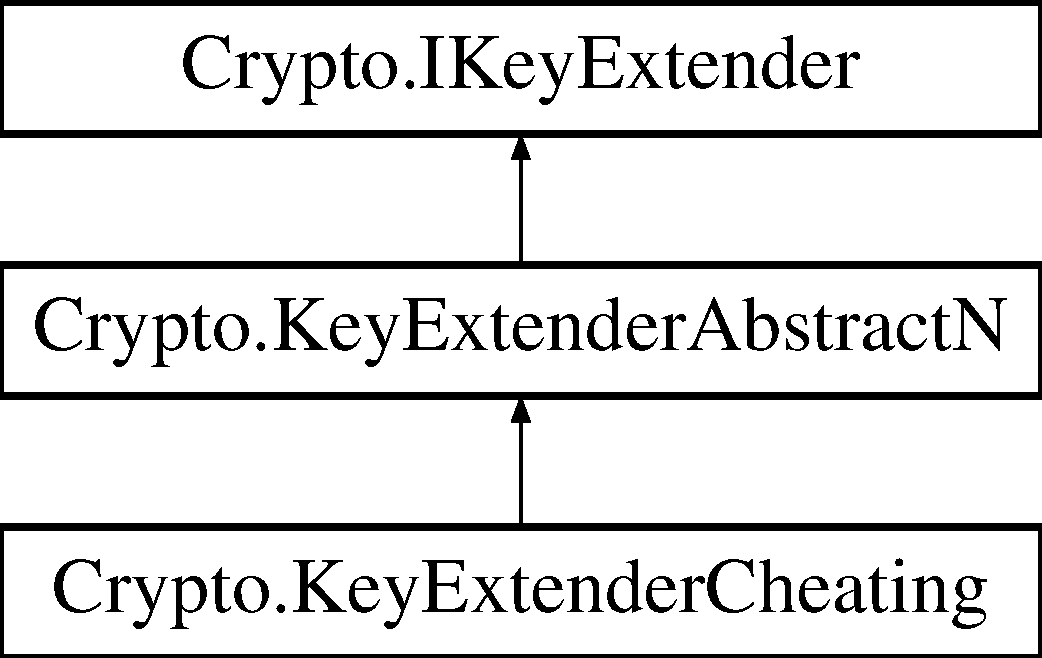
\includegraphics[height=3.000000cm]{class_crypto_1_1_key_extender_cheating}
\end{center}
\end{figure}
\subsection*{Public Member Functions}
\begin{DoxyCompactItemize}
\item 
override Bit\+Array \hyperlink{class_crypto_1_1_key_extender_cheating_a8018900fc6f660f83cb7cd23d52b60a3}{Extend\+Key} (Bit\+Array short\+Key, int target\+Length)
\begin{DoxyCompactList}\small\item\em Generates a longer key from a short key. \end{DoxyCompactList}\end{DoxyCompactItemize}


\subsection{Detailed Description}
Fake key extender which only generates random long key independently of the short key. 



Definition at line 9 of file Key\+Extender\+Cheating.\+cs.



\subsection{Member Function Documentation}
\hypertarget{class_crypto_1_1_key_extender_cheating_a8018900fc6f660f83cb7cd23d52b60a3}{}\index{Crypto\+::\+Key\+Extender\+Cheating@{Crypto\+::\+Key\+Extender\+Cheating}!Extend\+Key@{Extend\+Key}}
\index{Extend\+Key@{Extend\+Key}!Crypto\+::\+Key\+Extender\+Cheating@{Crypto\+::\+Key\+Extender\+Cheating}}
\subsubsection[{Extend\+Key(\+Bit\+Array short\+Key, int target\+Length)}]{\setlength{\rightskip}{0pt plus 5cm}override Bit\+Array Crypto.\+Key\+Extender\+Cheating.\+Extend\+Key (
\begin{DoxyParamCaption}
\item[{Bit\+Array}]{short\+Key, }
\item[{int}]{target\+Length}
\end{DoxyParamCaption}
)\hspace{0.3cm}{\ttfamily [virtual]}}\label{class_crypto_1_1_key_extender_cheating_a8018900fc6f660f83cb7cd23d52b60a3}


Generates a longer key from a short key. 


\begin{DoxyParams}{Parameters}
{\em short\+Key} & Short key to be stretched (multiplied).\\
\hline
{\em target\+Length} & How many bits should the resulting long key have?\\
\hline
\end{DoxyParams}
\begin{DoxyReturn}{Returns}
Long key (of specified length).
\end{DoxyReturn}


Implements \hyperlink{class_crypto_1_1_key_extender_abstract_n_a9df4156ad0a84730f87119e5a25cf1ef}{Crypto.\+Key\+Extender\+Abstract\+N}.



Definition at line 11 of file Key\+Extender\+Cheating.\+cs.



The documentation for this class was generated from the following file\+:\begin{DoxyCompactItemize}
\item 
C\+:/\+Martin/\+M\+F\+F/\+\_\+baka/\+Martin\+Dvorak/\+Crypto/\hyperlink{_key_extender_cheating_8cs}{Key\+Extender\+Cheating.\+cs}\end{DoxyCompactItemize}

\hypertarget{class_crypto_1_1_key_extender_copy}{}\section{Crypto.\+Key\+Extender\+Copy Class Reference}
\label{class_crypto_1_1_key_extender_copy}\index{Crypto.\+Key\+Extender\+Copy@{Crypto.\+Key\+Extender\+Copy}}


Stupid key extender which only copies the input (repeatedly).  


Inheritance diagram for Crypto.\+Key\+Extender\+Copy\+:\begin{figure}[H]
\begin{center}
\leavevmode
\includegraphics[height=3.000000cm]{class_crypto_1_1_key_extender_copy}
\end{center}
\end{figure}
\subsection*{Public Member Functions}
\begin{DoxyCompactItemize}
\item 
override Bit\+Array \hyperlink{class_crypto_1_1_key_extender_copy_ab57d10f5c80bbf6ab395e0a0b690080a}{Double\+Key} (Bit\+Array short\+Key)
\begin{DoxyCompactList}\small\item\em Generates a longer key from a short key. \end{DoxyCompactList}\end{DoxyCompactItemize}
\subsection*{Package Functions}
\begin{DoxyCompactItemize}
\item 
override string \hyperlink{class_crypto_1_1_key_extender_copy_ab6904bc5e3596cb7ac2cd7840cf356ef}{Get\+Info} ()
\end{DoxyCompactItemize}


\subsection{Detailed Description}
Stupid key extender which only copies the input (repeatedly). 



Definition at line 8 of file Key\+Extender\+Copy.\+cs.



\subsection{Member Function Documentation}
\hypertarget{class_crypto_1_1_key_extender_copy_ab57d10f5c80bbf6ab395e0a0b690080a}{}\index{Crypto\+::\+Key\+Extender\+Copy@{Crypto\+::\+Key\+Extender\+Copy}!Double\+Key@{Double\+Key}}
\index{Double\+Key@{Double\+Key}!Crypto\+::\+Key\+Extender\+Copy@{Crypto\+::\+Key\+Extender\+Copy}}
\subsubsection[{Double\+Key(\+Bit\+Array short\+Key)}]{\setlength{\rightskip}{0pt plus 5cm}override Bit\+Array Crypto.\+Key\+Extender\+Copy.\+Double\+Key (
\begin{DoxyParamCaption}
\item[{Bit\+Array}]{short\+Key}
\end{DoxyParamCaption}
)\hspace{0.3cm}{\ttfamily [virtual]}}\label{class_crypto_1_1_key_extender_copy_ab57d10f5c80bbf6ab395e0a0b690080a}


Generates a longer key from a short key. 


\begin{DoxyParams}{Parameters}
{\em short\+Key} & Short key to be stretched (doubled).\\
\hline
\end{DoxyParams}
\begin{DoxyReturn}{Returns}
Long key (twice longer than input).
\end{DoxyReturn}


Implements \hyperlink{class_crypto_1_1_key_extender_abstract_d_ae403b92e9038b9c0bc7a21885e24ffc7}{Crypto.\+Key\+Extender\+Abstract\+D}.



Definition at line 10 of file Key\+Extender\+Copy.\+cs.

\hypertarget{class_crypto_1_1_key_extender_copy_ab6904bc5e3596cb7ac2cd7840cf356ef}{}\index{Crypto\+::\+Key\+Extender\+Copy@{Crypto\+::\+Key\+Extender\+Copy}!Get\+Info@{Get\+Info}}
\index{Get\+Info@{Get\+Info}!Crypto\+::\+Key\+Extender\+Copy@{Crypto\+::\+Key\+Extender\+Copy}}
\subsubsection[{Get\+Info()}]{\setlength{\rightskip}{0pt plus 5cm}override string Crypto.\+Key\+Extender\+Copy.\+Get\+Info (
\begin{DoxyParamCaption}
{}
\end{DoxyParamCaption}
)\hspace{0.3cm}{\ttfamily [package]}, {\ttfamily [virtual]}}\label{class_crypto_1_1_key_extender_copy_ab6904bc5e3596cb7ac2cd7840cf356ef}


Implements \hyperlink{class_crypto_1_1_key_extender_abstract_d_a954261bd6f533ad7745beac9ce89dd6e}{Crypto.\+Key\+Extender\+Abstract\+D}.



Definition at line 22 of file Key\+Extender\+Copy.\+cs.



The documentation for this class was generated from the following file\+:\begin{DoxyCompactItemize}
\item 
C\+:/\+Martin/\+M\+F\+F/\+\_\+baka/\+Martin\+Dvorak/\+Crypto/\hyperlink{_key_extender_copy_8cs}{Key\+Extender\+Copy.\+cs}\end{DoxyCompactItemize}

\hypertarget{class_crypto_1_1_key_extender_genetic}{}\section{Crypto.\+Key\+Extender\+Genetic Class Reference}
\label{class_crypto_1_1_key_extender_genetic}\index{Crypto.\+Key\+Extender\+Genetic@{Crypto.\+Key\+Extender\+Genetic}}


Algorithms which runs a genetic algorithm to find the best sequence of extenders for each key. Generating the long key may take a very long time.  


Inheritance diagram for Crypto.\+Key\+Extender\+Genetic\+:\begin{figure}[H]
\begin{center}
\leavevmode
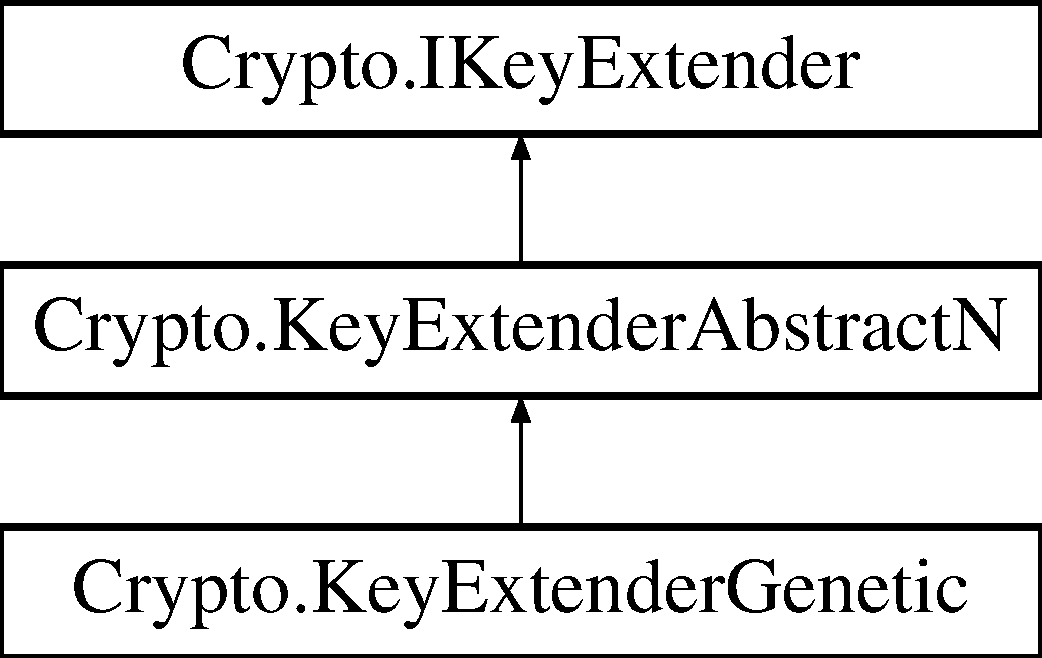
\includegraphics[height=3.000000cm]{class_crypto_1_1_key_extender_genetic}
\end{center}
\end{figure}
\subsection*{Public Member Functions}
\begin{DoxyCompactItemize}
\item 
\hyperlink{class_crypto_1_1_key_extender_genetic_a60bbe95f9ec44c270006a901acf199e5}{Key\+Extender\+Genetic} ()
\end{DoxyCompactItemize}


\subsection{Detailed Description}
Algorithms which runs a genetic algorithm to find the best sequence of extenders for each key. Generating the long key may take a very long time. 



Definition at line 13 of file Key\+Extender\+Genetic.\+cs.



\subsection{Constructor \& Destructor Documentation}
\hypertarget{class_crypto_1_1_key_extender_genetic_a60bbe95f9ec44c270006a901acf199e5}{}\index{Crypto\+::\+Key\+Extender\+Genetic@{Crypto\+::\+Key\+Extender\+Genetic}!Key\+Extender\+Genetic@{Key\+Extender\+Genetic}}
\index{Key\+Extender\+Genetic@{Key\+Extender\+Genetic}!Crypto\+::\+Key\+Extender\+Genetic@{Crypto\+::\+Key\+Extender\+Genetic}}
\subsubsection[{Key\+Extender\+Genetic()}]{\setlength{\rightskip}{0pt plus 5cm}Crypto.\+Key\+Extender\+Genetic.\+Key\+Extender\+Genetic (
\begin{DoxyParamCaption}
{}
\end{DoxyParamCaption}
)}\label{class_crypto_1_1_key_extender_genetic_a60bbe95f9ec44c270006a901acf199e5}


Definition at line 64 of file Key\+Extender\+Genetic.\+cs.



The documentation for this class was generated from the following file\+:\begin{DoxyCompactItemize}
\item 
C\+:/\+Martin/\+M\+F\+F/\+\_\+baka/\+Martin\+Dvorak/\+Crypto/\hyperlink{_key_extender_genetic_8cs}{Key\+Extender\+Genetic.\+cs}\end{DoxyCompactItemize}

\hypertarget{class_crypto_1_1_key_extender_interlaced}{}\section{Crypto.\+Key\+Extender\+Interlaced Class Reference}
\label{class_crypto_1_1_key_extender_interlaced}\index{Crypto.\+Key\+Extender\+Interlaced@{Crypto.\+Key\+Extender\+Interlaced}}


Different linear algorithm, which uses specified number of steps of the underlying C\+A.  


Inheritance diagram for Crypto.\+Key\+Extender\+Interlaced\+:\begin{figure}[H]
\begin{center}
\leavevmode
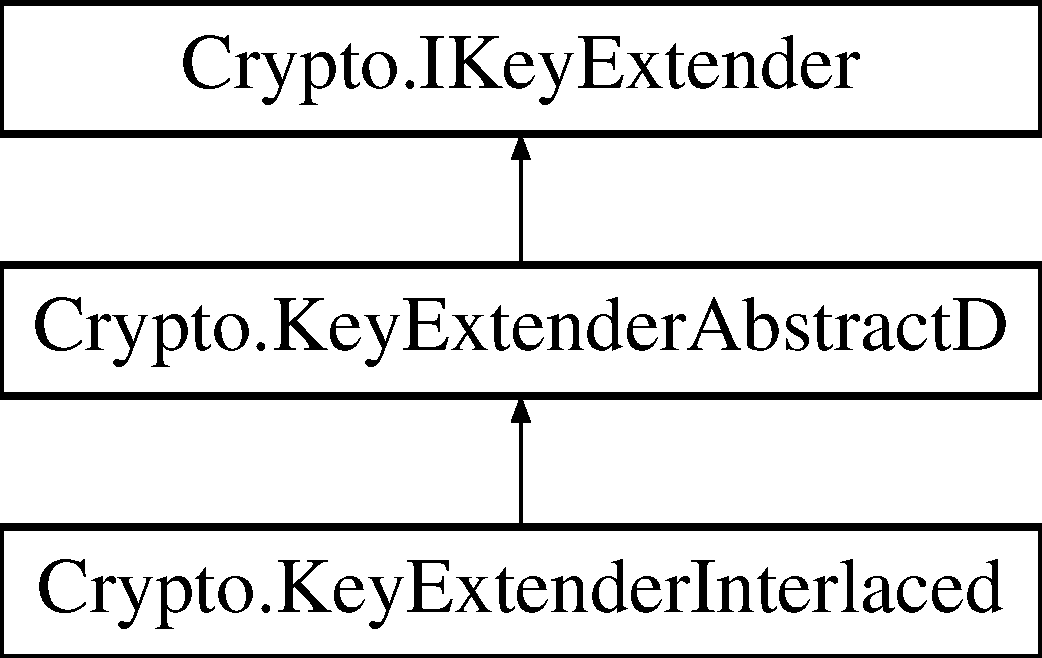
\includegraphics[height=3.000000cm]{class_crypto_1_1_key_extender_interlaced}
\end{center}
\end{figure}
\subsection*{Public Member Functions}
\begin{DoxyCompactItemize}
\item 
\hyperlink{class_crypto_1_1_key_extender_interlaced_a00ed5af7a686d03b60fa8c3607c27d6b}{Key\+Extender\+Interlaced} (\hyperlink{interface_cellular_1_1_i_binary_c_a}{I\+Binary\+C\+A} binary\+C\+A, int row\+Count, int skip\+Count)
\begin{DoxyCompactList}\small\item\em Creates a new \hyperlink{class_crypto_1_1_key_extender_interlaced}{Key\+Extender\+Interlaced}. \end{DoxyCompactList}\item 
override Bit\+Array \hyperlink{class_crypto_1_1_key_extender_interlaced_a1caf1b3ad04b24305f964ab44a399751}{Double\+Key} (Bit\+Array short\+Key)
\begin{DoxyCompactList}\small\item\em Generates a longer key from a short key. \end{DoxyCompactList}\end{DoxyCompactItemize}


\subsection{Detailed Description}
Different linear algorithm, which uses specified number of steps of the underlying C\+A. 



Definition at line 10 of file Key\+Extender\+Interlaced.\+cs.



\subsection{Constructor \& Destructor Documentation}
\hypertarget{class_crypto_1_1_key_extender_interlaced_a00ed5af7a686d03b60fa8c3607c27d6b}{}\index{Crypto\+::\+Key\+Extender\+Interlaced@{Crypto\+::\+Key\+Extender\+Interlaced}!Key\+Extender\+Interlaced@{Key\+Extender\+Interlaced}}
\index{Key\+Extender\+Interlaced@{Key\+Extender\+Interlaced}!Crypto\+::\+Key\+Extender\+Interlaced@{Crypto\+::\+Key\+Extender\+Interlaced}}
\subsubsection[{Key\+Extender\+Interlaced(\+I\+Binary\+C\+A binary\+C\+A, int row\+Count, int skip\+Count)}]{\setlength{\rightskip}{0pt plus 5cm}Crypto.\+Key\+Extender\+Interlaced.\+Key\+Extender\+Interlaced (
\begin{DoxyParamCaption}
\item[{{\bf I\+Binary\+C\+A}}]{binary\+C\+A, }
\item[{int}]{row\+Count, }
\item[{int}]{skip\+Count}
\end{DoxyParamCaption}
)}\label{class_crypto_1_1_key_extender_interlaced_a00ed5af7a686d03b60fa8c3607c27d6b}


Creates a new \hyperlink{class_crypto_1_1_key_extender_interlaced}{Key\+Extender\+Interlaced}. 


\begin{DoxyParams}{Parameters}
{\em binary\+C\+A} & What cellular automaton should be used to generate keys.\\
\hline
{\em row\+Count} & How many different rows should be used to generate keys.\\
\hline
{\em skip\+Count} & How many extra steps of the underlying C\+A should be performed between every use.\\
\hline
\end{DoxyParams}


Definition at line 22 of file Key\+Extender\+Interlaced.\+cs.



\subsection{Member Function Documentation}
\hypertarget{class_crypto_1_1_key_extender_interlaced_a1caf1b3ad04b24305f964ab44a399751}{}\index{Crypto\+::\+Key\+Extender\+Interlaced@{Crypto\+::\+Key\+Extender\+Interlaced}!Double\+Key@{Double\+Key}}
\index{Double\+Key@{Double\+Key}!Crypto\+::\+Key\+Extender\+Interlaced@{Crypto\+::\+Key\+Extender\+Interlaced}}
\subsubsection[{Double\+Key(\+Bit\+Array short\+Key)}]{\setlength{\rightskip}{0pt plus 5cm}override Bit\+Array Crypto.\+Key\+Extender\+Interlaced.\+Double\+Key (
\begin{DoxyParamCaption}
\item[{Bit\+Array}]{short\+Key}
\end{DoxyParamCaption}
)\hspace{0.3cm}{\ttfamily [virtual]}}\label{class_crypto_1_1_key_extender_interlaced_a1caf1b3ad04b24305f964ab44a399751}


Generates a longer key from a short key. 


\begin{DoxyParams}{Parameters}
{\em short\+Key} & Short key to be stretched (doubled).\\
\hline
\end{DoxyParams}
\begin{DoxyReturn}{Returns}
Long key (twice longer than input).
\end{DoxyReturn}


Implements \hyperlink{class_crypto_1_1_key_extender_abstract_d_ae403b92e9038b9c0bc7a21885e24ffc7}{Crypto.\+Key\+Extender\+Abstract\+D}.



Definition at line 33 of file Key\+Extender\+Interlaced.\+cs.



The documentation for this class was generated from the following file\+:\begin{DoxyCompactItemize}
\item 
C\+:/\+Martin/\+M\+F\+F/\+\_\+baka/\+Martin\+Dvorak/\+Crypto/\hyperlink{_key_extender_interlaced_8cs}{Key\+Extender\+Interlaced.\+cs}\end{DoxyCompactItemize}

\hypertarget{class_crypto_1_1_key_extender_simple_linear}{}\section{Crypto.\+Key\+Extender\+Simple\+Linear Class Reference}
\label{class_crypto_1_1_key_extender_simple_linear}\index{Crypto.\+Key\+Extender\+Simple\+Linear@{Crypto.\+Key\+Extender\+Simple\+Linear}}


Simple algorithm, which uses only two steps of the underlying C\+A.  


Inheritance diagram for Crypto.\+Key\+Extender\+Simple\+Linear\+:\begin{figure}[H]
\begin{center}
\leavevmode
\includegraphics[height=3.000000cm]{class_crypto_1_1_key_extender_simple_linear}
\end{center}
\end{figure}
\subsection*{Public Member Functions}
\begin{DoxyCompactItemize}
\item 
\hyperlink{class_crypto_1_1_key_extender_simple_linear_a318ebefc5ef25570e751b21c071fba06}{Key\+Extender\+Simple\+Linear} (\hyperlink{interface_cellular_1_1_i_binary_c_a}{I\+Binary\+C\+A} binary\+C\+A)
\item 
override Bit\+Array \hyperlink{class_crypto_1_1_key_extender_simple_linear_a1b511ea8a0e0bb6cbd4f6a94f49015bd}{Double\+Key} (Bit\+Array short\+Key)
\begin{DoxyCompactList}\small\item\em Generates a longer key from a short key. \end{DoxyCompactList}\end{DoxyCompactItemize}


\subsection{Detailed Description}
Simple algorithm, which uses only two steps of the underlying C\+A. 



Definition at line 9 of file Key\+Extender\+Simple\+Linear.\+cs.



\subsection{Constructor \& Destructor Documentation}
\hypertarget{class_crypto_1_1_key_extender_simple_linear_a318ebefc5ef25570e751b21c071fba06}{}\index{Crypto\+::\+Key\+Extender\+Simple\+Linear@{Crypto\+::\+Key\+Extender\+Simple\+Linear}!Key\+Extender\+Simple\+Linear@{Key\+Extender\+Simple\+Linear}}
\index{Key\+Extender\+Simple\+Linear@{Key\+Extender\+Simple\+Linear}!Crypto\+::\+Key\+Extender\+Simple\+Linear@{Crypto\+::\+Key\+Extender\+Simple\+Linear}}
\subsubsection[{Key\+Extender\+Simple\+Linear(\+I\+Binary\+C\+A binary\+C\+A)}]{\setlength{\rightskip}{0pt plus 5cm}Crypto.\+Key\+Extender\+Simple\+Linear.\+Key\+Extender\+Simple\+Linear (
\begin{DoxyParamCaption}
\item[{{\bf I\+Binary\+C\+A}}]{binary\+C\+A}
\end{DoxyParamCaption}
)}\label{class_crypto_1_1_key_extender_simple_linear_a318ebefc5ef25570e751b21c071fba06}


Definition at line 13 of file Key\+Extender\+Simple\+Linear.\+cs.



\subsection{Member Function Documentation}
\hypertarget{class_crypto_1_1_key_extender_simple_linear_a1b511ea8a0e0bb6cbd4f6a94f49015bd}{}\index{Crypto\+::\+Key\+Extender\+Simple\+Linear@{Crypto\+::\+Key\+Extender\+Simple\+Linear}!Double\+Key@{Double\+Key}}
\index{Double\+Key@{Double\+Key}!Crypto\+::\+Key\+Extender\+Simple\+Linear@{Crypto\+::\+Key\+Extender\+Simple\+Linear}}
\subsubsection[{Double\+Key(\+Bit\+Array short\+Key)}]{\setlength{\rightskip}{0pt plus 5cm}override Bit\+Array Crypto.\+Key\+Extender\+Simple\+Linear.\+Double\+Key (
\begin{DoxyParamCaption}
\item[{Bit\+Array}]{short\+Key}
\end{DoxyParamCaption}
)\hspace{0.3cm}{\ttfamily [virtual]}}\label{class_crypto_1_1_key_extender_simple_linear_a1b511ea8a0e0bb6cbd4f6a94f49015bd}


Generates a longer key from a short key. 


\begin{DoxyParams}{Parameters}
{\em short\+Key} & Short key to be stretched (doubled).\\
\hline
\end{DoxyParams}
\begin{DoxyReturn}{Returns}
Long key (twice longer than input).
\end{DoxyReturn}


Implements \hyperlink{class_crypto_1_1_key_extender_abstract_d_ae403b92e9038b9c0bc7a21885e24ffc7}{Crypto.\+Key\+Extender\+Abstract\+D}.



Definition at line 18 of file Key\+Extender\+Simple\+Linear.\+cs.



The documentation for this class was generated from the following file\+:\begin{DoxyCompactItemize}
\item 
C\+:/\+Martin/\+M\+F\+F/\+\_\+baka/\+Martin\+Dvorak/\+Crypto/\hyperlink{_key_extender_simple_linear_8cs}{Key\+Extender\+Simple\+Linear.\+cs}\end{DoxyCompactItemize}

\hypertarget{class_crypto_1_1_key_extender_simple_quadratic}{}\section{Crypto.\+Key\+Extender\+Simple\+Quadratic Class Reference}
\label{class_crypto_1_1_key_extender_simple_quadratic}\index{Crypto.\+Key\+Extender\+Simple\+Quadratic@{Crypto.\+Key\+Extender\+Simple\+Quadratic}}


Simple algorithm, which calls one step of the underlying C\+A for every bit to be generated. Generating the long key may take a very long time.  


Inheritance diagram for Crypto.\+Key\+Extender\+Simple\+Quadratic\+:\begin{figure}[H]
\begin{center}
\leavevmode
\includegraphics[height=3.000000cm]{class_crypto_1_1_key_extender_simple_quadratic}
\end{center}
\end{figure}
\subsection*{Public Member Functions}
\begin{DoxyCompactItemize}
\item 
\hyperlink{class_crypto_1_1_key_extender_simple_quadratic_a2090b48093409cd09a18c56ac7ec7826}{Key\+Extender\+Simple\+Quadratic} (\hyperlink{interface_cellular_1_1_i_binary_c_a}{I\+Binary\+C\+A} binary\+C\+A)
\item 
override Bit\+Array \hyperlink{class_crypto_1_1_key_extender_simple_quadratic_a0bba7646011678850879c0685d18b379}{Double\+Key} (Bit\+Array short\+Key)
\begin{DoxyCompactList}\small\item\em Generates a longer key from a short key. \end{DoxyCompactList}\end{DoxyCompactItemize}
\subsection*{Package Functions}
\begin{DoxyCompactItemize}
\item 
override string \hyperlink{class_crypto_1_1_key_extender_simple_quadratic_a4a399b40cd1893acf4cc8531771657a0}{Get\+Info} ()
\end{DoxyCompactItemize}


\subsection{Detailed Description}
Simple algorithm, which calls one step of the underlying C\+A for every bit to be generated. Generating the long key may take a very long time. 



Definition at line 10 of file Key\+Extender\+Simple\+Quadratic.\+cs.



\subsection{Constructor \& Destructor Documentation}
\hypertarget{class_crypto_1_1_key_extender_simple_quadratic_a2090b48093409cd09a18c56ac7ec7826}{}\index{Crypto\+::\+Key\+Extender\+Simple\+Quadratic@{Crypto\+::\+Key\+Extender\+Simple\+Quadratic}!Key\+Extender\+Simple\+Quadratic@{Key\+Extender\+Simple\+Quadratic}}
\index{Key\+Extender\+Simple\+Quadratic@{Key\+Extender\+Simple\+Quadratic}!Crypto\+::\+Key\+Extender\+Simple\+Quadratic@{Crypto\+::\+Key\+Extender\+Simple\+Quadratic}}
\subsubsection[{Key\+Extender\+Simple\+Quadratic(\+I\+Binary\+C\+A binary\+C\+A)}]{\setlength{\rightskip}{0pt plus 5cm}Crypto.\+Key\+Extender\+Simple\+Quadratic.\+Key\+Extender\+Simple\+Quadratic (
\begin{DoxyParamCaption}
\item[{{\bf I\+Binary\+C\+A}}]{binary\+C\+A}
\end{DoxyParamCaption}
)}\label{class_crypto_1_1_key_extender_simple_quadratic_a2090b48093409cd09a18c56ac7ec7826}


Definition at line 14 of file Key\+Extender\+Simple\+Quadratic.\+cs.



\subsection{Member Function Documentation}
\hypertarget{class_crypto_1_1_key_extender_simple_quadratic_a0bba7646011678850879c0685d18b379}{}\index{Crypto\+::\+Key\+Extender\+Simple\+Quadratic@{Crypto\+::\+Key\+Extender\+Simple\+Quadratic}!Double\+Key@{Double\+Key}}
\index{Double\+Key@{Double\+Key}!Crypto\+::\+Key\+Extender\+Simple\+Quadratic@{Crypto\+::\+Key\+Extender\+Simple\+Quadratic}}
\subsubsection[{Double\+Key(\+Bit\+Array short\+Key)}]{\setlength{\rightskip}{0pt plus 5cm}override Bit\+Array Crypto.\+Key\+Extender\+Simple\+Quadratic.\+Double\+Key (
\begin{DoxyParamCaption}
\item[{Bit\+Array}]{short\+Key}
\end{DoxyParamCaption}
)\hspace{0.3cm}{\ttfamily [virtual]}}\label{class_crypto_1_1_key_extender_simple_quadratic_a0bba7646011678850879c0685d18b379}


Generates a longer key from a short key. 


\begin{DoxyParams}{Parameters}
{\em short\+Key} & Short key to be stretched (doubled).\\
\hline
\end{DoxyParams}
\begin{DoxyReturn}{Returns}
Long key (twice longer than input).
\end{DoxyReturn}


Implements \hyperlink{class_crypto_1_1_key_extender_abstract_d_ae403b92e9038b9c0bc7a21885e24ffc7}{Crypto.\+Key\+Extender\+Abstract\+D}.



Definition at line 19 of file Key\+Extender\+Simple\+Quadratic.\+cs.

\hypertarget{class_crypto_1_1_key_extender_simple_quadratic_a4a399b40cd1893acf4cc8531771657a0}{}\index{Crypto\+::\+Key\+Extender\+Simple\+Quadratic@{Crypto\+::\+Key\+Extender\+Simple\+Quadratic}!Get\+Info@{Get\+Info}}
\index{Get\+Info@{Get\+Info}!Crypto\+::\+Key\+Extender\+Simple\+Quadratic@{Crypto\+::\+Key\+Extender\+Simple\+Quadratic}}
\subsubsection[{Get\+Info()}]{\setlength{\rightskip}{0pt plus 5cm}override string Crypto.\+Key\+Extender\+Simple\+Quadratic.\+Get\+Info (
\begin{DoxyParamCaption}
{}
\end{DoxyParamCaption}
)\hspace{0.3cm}{\ttfamily [package]}, {\ttfamily [virtual]}}\label{class_crypto_1_1_key_extender_simple_quadratic_a4a399b40cd1893acf4cc8531771657a0}


Implements \hyperlink{class_crypto_1_1_key_extender_abstract_d_a954261bd6f533ad7745beac9ce89dd6e}{Crypto.\+Key\+Extender\+Abstract\+D}.



Definition at line 40 of file Key\+Extender\+Simple\+Quadratic.\+cs.



The documentation for this class was generated from the following file\+:\begin{DoxyCompactItemize}
\item 
C\+:/\+Martin/\+M\+F\+F/\+\_\+baka/\+Martin\+Dvorak/\+Crypto/\hyperlink{_key_extender_simple_quadratic_8cs}{Key\+Extender\+Simple\+Quadratic.\+cs}\end{DoxyCompactItemize}

\hypertarget{class_crypto_1_1_key_extender_uncertain}{}\section{Crypto.\+Key\+Extender\+Uncertain Class Reference}
\label{class_crypto_1_1_key_extender_uncertain}\index{Crypto.\+Key\+Extender\+Uncertain@{Crypto.\+Key\+Extender\+Uncertain}}


Intelligent key extender that equalizes frequencies of 0 and 1, which may be different in the underlying C\+A. However it is not guaranteed that the long key will be generated.  


Inheritance diagram for Crypto.\+Key\+Extender\+Uncertain\+:\begin{figure}[H]
\begin{center}
\leavevmode
\includegraphics[height=3.000000cm]{class_crypto_1_1_key_extender_uncertain}
\end{center}
\end{figure}
\subsection*{Public Member Functions}
\begin{DoxyCompactItemize}
\item 
\hyperlink{class_crypto_1_1_key_extender_uncertain_aace64d24b92154a9e01002ee13e0b891}{Key\+Extender\+Uncertain} (\hyperlink{interface_cellular_1_1_i_binary_c_a}{I\+Binary\+C\+A} binary\+C\+A)
\item 
override Bit\+Array \hyperlink{class_crypto_1_1_key_extender_uncertain_a2955df98d2f4831576b12aa9c5ec609d}{Extend\+Key} (Bit\+Array short\+Key, int target\+Length)
\begin{DoxyCompactList}\small\item\em Generates a longer key from a short key. \end{DoxyCompactList}\end{DoxyCompactItemize}


\subsection{Detailed Description}
Intelligent key extender that equalizes frequencies of 0 and 1, which may be different in the underlying C\+A. However it is not guaranteed that the long key will be generated. 



Definition at line 10 of file Key\+Extender\+Uncertain.\+cs.



\subsection{Constructor \& Destructor Documentation}
\hypertarget{class_crypto_1_1_key_extender_uncertain_aace64d24b92154a9e01002ee13e0b891}{}\index{Crypto\+::\+Key\+Extender\+Uncertain@{Crypto\+::\+Key\+Extender\+Uncertain}!Key\+Extender\+Uncertain@{Key\+Extender\+Uncertain}}
\index{Key\+Extender\+Uncertain@{Key\+Extender\+Uncertain}!Crypto\+::\+Key\+Extender\+Uncertain@{Crypto\+::\+Key\+Extender\+Uncertain}}
\subsubsection[{Key\+Extender\+Uncertain(\+I\+Binary\+C\+A binary\+C\+A)}]{\setlength{\rightskip}{0pt plus 5cm}Crypto.\+Key\+Extender\+Uncertain.\+Key\+Extender\+Uncertain (
\begin{DoxyParamCaption}
\item[{{\bf I\+Binary\+C\+A}}]{binary\+C\+A}
\end{DoxyParamCaption}
)}\label{class_crypto_1_1_key_extender_uncertain_aace64d24b92154a9e01002ee13e0b891}


Definition at line 14 of file Key\+Extender\+Uncertain.\+cs.



\subsection{Member Function Documentation}
\hypertarget{class_crypto_1_1_key_extender_uncertain_a2955df98d2f4831576b12aa9c5ec609d}{}\index{Crypto\+::\+Key\+Extender\+Uncertain@{Crypto\+::\+Key\+Extender\+Uncertain}!Extend\+Key@{Extend\+Key}}
\index{Extend\+Key@{Extend\+Key}!Crypto\+::\+Key\+Extender\+Uncertain@{Crypto\+::\+Key\+Extender\+Uncertain}}
\subsubsection[{Extend\+Key(\+Bit\+Array short\+Key, int target\+Length)}]{\setlength{\rightskip}{0pt plus 5cm}override Bit\+Array Crypto.\+Key\+Extender\+Uncertain.\+Extend\+Key (
\begin{DoxyParamCaption}
\item[{Bit\+Array}]{short\+Key, }
\item[{int}]{target\+Length}
\end{DoxyParamCaption}
)\hspace{0.3cm}{\ttfamily [virtual]}}\label{class_crypto_1_1_key_extender_uncertain_a2955df98d2f4831576b12aa9c5ec609d}


Generates a longer key from a short key. 


\begin{DoxyParams}{Parameters}
{\em short\+Key} & Short key to be stretched (multiplied).\\
\hline
{\em target\+Length} & How many bits should the resulting long key have?\\
\hline
\end{DoxyParams}
\begin{DoxyReturn}{Returns}
Long key (of specified length).
\end{DoxyReturn}


Implements \hyperlink{class_crypto_1_1_key_extender_abstract_n_a9df4156ad0a84730f87119e5a25cf1ef}{Crypto.\+Key\+Extender\+Abstract\+N}.



Definition at line 19 of file Key\+Extender\+Uncertain.\+cs.



The documentation for this class was generated from the following file\+:\begin{DoxyCompactItemize}
\item 
C\+:/\+Martin/\+M\+F\+F/\+\_\+baka/\+Martin\+Dvorak/\+Crypto/\hyperlink{_key_extender_uncertain_8cs}{Key\+Extender\+Uncertain.\+cs}\end{DoxyCompactItemize}

\hypertarget{class_testing_1_1_main_tests}{}\section{Testing.\+Main\+Tests Class Reference}
\label{class_testing_1_1_main_tests}\index{Testing.\+Main\+Tests@{Testing.\+Main\+Tests}}


The most important tests (rating of key extenders) for my thesis.  


\subsection*{Static Public Member Functions}
\begin{DoxyCompactItemize}
\item 
static void \hyperlink{class_testing_1_1_main_tests_a013daeb576cbc0d58dfc82d8f5003806}{Run\+Test} ()
\begin{DoxyCompactList}\small\item\em Runs the most important tests for my thesis. \end{DoxyCompactList}\end{DoxyCompactItemize}


\subsection{Detailed Description}
The most important tests (rating of key extenders) for my thesis. 



Definition at line 11 of file Main\+Tests.\+cs.



\subsection{Member Function Documentation}
\hypertarget{class_testing_1_1_main_tests_a013daeb576cbc0d58dfc82d8f5003806}{}\index{Testing\+::\+Main\+Tests@{Testing\+::\+Main\+Tests}!Run\+Test@{Run\+Test}}
\index{Run\+Test@{Run\+Test}!Testing\+::\+Main\+Tests@{Testing\+::\+Main\+Tests}}
\subsubsection[{Run\+Test()}]{\setlength{\rightskip}{0pt plus 5cm}static void Testing.\+Main\+Tests.\+Run\+Test (
\begin{DoxyParamCaption}
{}
\end{DoxyParamCaption}
)\hspace{0.3cm}{\ttfamily [static]}}\label{class_testing_1_1_main_tests_a013daeb576cbc0d58dfc82d8f5003806}


Runs the most important tests for my thesis. 



Definition at line 16 of file Main\+Tests.\+cs.



The documentation for this class was generated from the following file\+:\begin{DoxyCompactItemize}
\item 
C\+:/\+Martin/\+M\+F\+F/\+\_\+baka/\+Martin\+Dvorak/\+Testing/\hyperlink{_main_tests_8cs}{Main\+Tests.\+cs}\end{DoxyCompactItemize}

\hypertarget{class_cellular_1_1_nary1_d_automaton}{}\section{Cellular.\+Nary1\+D\+Automaton Class Reference}
\label{class_cellular_1_1_nary1_d_automaton}\index{Cellular.\+Nary1\+D\+Automaton@{Cellular.\+Nary1\+D\+Automaton}}


Abstract class for general 1\+D N-\/ary automata.  


Inheritance diagram for Cellular.\+Nary1\+D\+Automaton\+:\begin{figure}[H]
\begin{center}
\leavevmode
\includegraphics[height=5.000000cm]{class_cellular_1_1_nary1_d_automaton}
\end{center}
\end{figure}
\subsection*{Public Member Functions}
\begin{DoxyCompactItemize}
\item 
\hyperlink{class_cellular_1_1_nary1_d_automaton_a9b38ab16780bc9fb347f714bdd8f1295}{Nary1\+D\+Automaton} (int number\+Of\+States, int\mbox{[}$\,$\mbox{]} \hyperlink{all__1_8js_ae8b87ff4be2ae1dd5267342795263360}{initial\+State})
\item 
\hyperlink{class_cellular_1_1_nary1_d_automaton_ad9678852ba9ef44a300f2d272757d482}{Nary1\+D\+Automaton} (int number\+Of\+States, int \hyperlink{class_cellular_1_1_automaton1_d_a915129ccf0f1e7092844c99ce6a28e5b}{size}, Random rnd)
\end{DoxyCompactItemize}
\subsection*{Protected Member Functions}
\begin{DoxyCompactItemize}
\item 
virtual int \hyperlink{class_cellular_1_1_nary1_d_automaton_adfd39915b66667efeeb9b16f154b9b6b}{get\+Value\+At} (int index)
\begin{DoxyCompactList}\small\item\em This method simplifies boundary conditions. \end{DoxyCompactList}\end{DoxyCompactItemize}
\subsection*{Protected Attributes}
\begin{DoxyCompactItemize}
\item 
int \hyperlink{class_cellular_1_1_nary1_d_automaton_a1e499082e289666a6eb3d523d367ac1f}{N}
\item 
int\mbox{[}$\,$\mbox{]} \hyperlink{class_cellular_1_1_nary1_d_automaton_a563eb68c941321814d9261d68eed63f3}{state}
\end{DoxyCompactItemize}


\subsection{Detailed Description}
Abstract class for general 1\+D N-\/ary automata. 



Definition at line 8 of file Nary1\+D\+Automaton.\+cs.



\subsection{Constructor \& Destructor Documentation}
\hypertarget{class_cellular_1_1_nary1_d_automaton_a9b38ab16780bc9fb347f714bdd8f1295}{}\index{Cellular\+::\+Nary1\+D\+Automaton@{Cellular\+::\+Nary1\+D\+Automaton}!Nary1\+D\+Automaton@{Nary1\+D\+Automaton}}
\index{Nary1\+D\+Automaton@{Nary1\+D\+Automaton}!Cellular\+::\+Nary1\+D\+Automaton@{Cellular\+::\+Nary1\+D\+Automaton}}
\subsubsection[{Nary1\+D\+Automaton(int number\+Of\+States, int[] initial\+State)}]{\setlength{\rightskip}{0pt plus 5cm}Cellular.\+Nary1\+D\+Automaton.\+Nary1\+D\+Automaton (
\begin{DoxyParamCaption}
\item[{int}]{number\+Of\+States, }
\item[{int\mbox{[}$\,$\mbox{]}}]{initial\+State}
\end{DoxyParamCaption}
)}\label{class_cellular_1_1_nary1_d_automaton_a9b38ab16780bc9fb347f714bdd8f1295}


Definition at line 13 of file Nary1\+D\+Automaton.\+cs.

\hypertarget{class_cellular_1_1_nary1_d_automaton_ad9678852ba9ef44a300f2d272757d482}{}\index{Cellular\+::\+Nary1\+D\+Automaton@{Cellular\+::\+Nary1\+D\+Automaton}!Nary1\+D\+Automaton@{Nary1\+D\+Automaton}}
\index{Nary1\+D\+Automaton@{Nary1\+D\+Automaton}!Cellular\+::\+Nary1\+D\+Automaton@{Cellular\+::\+Nary1\+D\+Automaton}}
\subsubsection[{Nary1\+D\+Automaton(int number\+Of\+States, int size, Random rnd)}]{\setlength{\rightskip}{0pt plus 5cm}Cellular.\+Nary1\+D\+Automaton.\+Nary1\+D\+Automaton (
\begin{DoxyParamCaption}
\item[{int}]{number\+Of\+States, }
\item[{int}]{size, }
\item[{Random}]{rnd}
\end{DoxyParamCaption}
)}\label{class_cellular_1_1_nary1_d_automaton_ad9678852ba9ef44a300f2d272757d482}


Definition at line 20 of file Nary1\+D\+Automaton.\+cs.



\subsection{Member Function Documentation}
\hypertarget{class_cellular_1_1_nary1_d_automaton_adfd39915b66667efeeb9b16f154b9b6b}{}\index{Cellular\+::\+Nary1\+D\+Automaton@{Cellular\+::\+Nary1\+D\+Automaton}!get\+Value\+At@{get\+Value\+At}}
\index{get\+Value\+At@{get\+Value\+At}!Cellular\+::\+Nary1\+D\+Automaton@{Cellular\+::\+Nary1\+D\+Automaton}}
\subsubsection[{get\+Value\+At(int index)}]{\setlength{\rightskip}{0pt plus 5cm}virtual int Cellular.\+Nary1\+D\+Automaton.\+get\+Value\+At (
\begin{DoxyParamCaption}
\item[{int}]{index}
\end{DoxyParamCaption}
)\hspace{0.3cm}{\ttfamily [protected]}, {\ttfamily [virtual]}}\label{class_cellular_1_1_nary1_d_automaton_adfd39915b66667efeeb9b16f154b9b6b}


This method simplifies boundary conditions. 


\begin{DoxyParams}{Parameters}
{\em index} & Zero-\/based index (which value is required).\\
\hline
\end{DoxyParams}
\begin{DoxyReturn}{Returns}
Value from 0 to N-\/1.
\end{DoxyReturn}


Reimplemented in \hyperlink{class_cellular_1_1_nary_totalistic_cyclic_automaton_a422dbcbd3e3cd3efdccc21724e7c6b01}{Cellular.\+Nary\+Totalistic\+Cyclic\+Automaton}.



Definition at line 35 of file Nary1\+D\+Automaton.\+cs.



\subsection{Member Data Documentation}
\hypertarget{class_cellular_1_1_nary1_d_automaton_a1e499082e289666a6eb3d523d367ac1f}{}\index{Cellular\+::\+Nary1\+D\+Automaton@{Cellular\+::\+Nary1\+D\+Automaton}!N@{N}}
\index{N@{N}!Cellular\+::\+Nary1\+D\+Automaton@{Cellular\+::\+Nary1\+D\+Automaton}}
\subsubsection[{N}]{\setlength{\rightskip}{0pt plus 5cm}int Cellular.\+Nary1\+D\+Automaton.\+N\hspace{0.3cm}{\ttfamily [protected]}}\label{class_cellular_1_1_nary1_d_automaton_a1e499082e289666a6eb3d523d367ac1f}


Definition at line 10 of file Nary1\+D\+Automaton.\+cs.

\hypertarget{class_cellular_1_1_nary1_d_automaton_a563eb68c941321814d9261d68eed63f3}{}\index{Cellular\+::\+Nary1\+D\+Automaton@{Cellular\+::\+Nary1\+D\+Automaton}!state@{state}}
\index{state@{state}!Cellular\+::\+Nary1\+D\+Automaton@{Cellular\+::\+Nary1\+D\+Automaton}}
\subsubsection[{state}]{\setlength{\rightskip}{0pt plus 5cm}int \mbox{[}$\,$\mbox{]} Cellular.\+Nary1\+D\+Automaton.\+state\hspace{0.3cm}{\ttfamily [protected]}}\label{class_cellular_1_1_nary1_d_automaton_a563eb68c941321814d9261d68eed63f3}


Definition at line 11 of file Nary1\+D\+Automaton.\+cs.



The documentation for this class was generated from the following file\+:\begin{DoxyCompactItemize}
\item 
C\+:/\+Martin/\+M\+F\+F/\+\_\+baka/\+Martin\+Dvorak/\+Cellular/\hyperlink{_nary1_d_automaton_8cs}{Nary1\+D\+Automaton.\+cs}\end{DoxyCompactItemize}

\hypertarget{class_cellular_1_1_nary_totalistic_automaton}{}\section{Cellular.\+Nary\+Totalistic\+Automaton Class Reference}
\label{class_cellular_1_1_nary_totalistic_automaton}\index{Cellular.\+Nary\+Totalistic\+Automaton@{Cellular.\+Nary\+Totalistic\+Automaton}}


Class representing any n-\/ary one-\/dimensional automaton with a totalistic rule -\/ bordered variant. The new state of each cell depends on the sum of its current state and the current state of adjecent cells.  


Inheritance diagram for Cellular.\+Nary\+Totalistic\+Automaton\+:\begin{figure}[H]
\begin{center}
\leavevmode
\includegraphics[height=5.000000cm]{class_cellular_1_1_nary_totalistic_automaton}
\end{center}
\end{figure}
\subsection*{Public Member Functions}
\begin{DoxyCompactItemize}
\item 
\hyperlink{class_cellular_1_1_nary_totalistic_automaton_aafe92ae99ccbb3591b128d6e720227f6}{Nary\+Totalistic\+Automaton} (int number\+Of\+States, int\mbox{[}$\,$\mbox{]} \hyperlink{class_cellular_1_1_nary_totalistic_automaton_a878c767c6823bd8ed8dc0f7d2ccb1fd2}{rule}, int\mbox{[}$\,$\mbox{]} \hyperlink{all__1_8js_ae8b87ff4be2ae1dd5267342795263360}{initial\+State})
\begin{DoxyCompactList}\small\item\em Creates a new totalistic N-\/ary automaton with given rule and initial state. \end{DoxyCompactList}\item 
override void \hyperlink{class_cellular_1_1_nary_totalistic_automaton_ad90769a438ab94b46d4750a571782056}{Step} ()
\begin{DoxyCompactList}\small\item\em Performs one step applying the specific rule for creating a new state. \end{DoxyCompactList}\item 
override object \hyperlink{class_cellular_1_1_nary_totalistic_automaton_a13f16113915ecec451fc4764a32044f9}{Clone} ()
\begin{DoxyCompactList}\small\item\em Creates an appropriate copy of the C\+A. Its type and the specific rule are always preserved. However, the time (number of steps executed on the specific instance) is set back to 0. \end{DoxyCompactList}\item 
override string \hyperlink{class_cellular_1_1_nary_totalistic_automaton_aa691c532a55638c7e3d0c125a4244773}{Tell\+Type} ()
\begin{DoxyCompactList}\small\item\em Announces the runtime type of the C\+A including info about its rule. It serves for debugging purposes. \end{DoxyCompactList}\item 
string \hyperlink{class_cellular_1_1_nary_totalistic_automaton_a239c8e21ae35741c4baadb96be21cec9}{Print\+Ternary} ()
\begin{DoxyCompactList}\small\item\em Converts the inner state into a well-\/printable string. This method works best for ternary (N=3) automata. \end{DoxyCompactList}\item 
string \hyperlink{class_cellular_1_1_nary_totalistic_automaton_aa9d5e154d625d8a8884221df45766145}{Print\+Quinary} ()
\begin{DoxyCompactList}\small\item\em Converts the inner state into a well-\/printable string. This method works best for quinary (N=5) automata. \end{DoxyCompactList}\end{DoxyCompactItemize}
\subsection*{Protected Attributes}
\begin{DoxyCompactItemize}
\item 
int\mbox{[}$\,$\mbox{]} \hyperlink{class_cellular_1_1_nary_totalistic_automaton_a878c767c6823bd8ed8dc0f7d2ccb1fd2}{rule}
\end{DoxyCompactItemize}
\subsection*{Additional Inherited Members}


\subsection{Detailed Description}
Class representing any n-\/ary one-\/dimensional automaton with a totalistic rule -\/ bordered variant. The new state of each cell depends on the sum of its current state and the current state of adjecent cells. 



Definition at line 9 of file Nary\+Totalistic\+Automaton.\+cs.



\subsection{Constructor \& Destructor Documentation}
\hypertarget{class_cellular_1_1_nary_totalistic_automaton_aafe92ae99ccbb3591b128d6e720227f6}{}\index{Cellular\+::\+Nary\+Totalistic\+Automaton@{Cellular\+::\+Nary\+Totalistic\+Automaton}!Nary\+Totalistic\+Automaton@{Nary\+Totalistic\+Automaton}}
\index{Nary\+Totalistic\+Automaton@{Nary\+Totalistic\+Automaton}!Cellular\+::\+Nary\+Totalistic\+Automaton@{Cellular\+::\+Nary\+Totalistic\+Automaton}}
\subsubsection[{Nary\+Totalistic\+Automaton(int number\+Of\+States, int[] rule, int[] initial\+State)}]{\setlength{\rightskip}{0pt plus 5cm}Cellular.\+Nary\+Totalistic\+Automaton.\+Nary\+Totalistic\+Automaton (
\begin{DoxyParamCaption}
\item[{int}]{number\+Of\+States, }
\item[{int\mbox{[}$\,$\mbox{]}}]{rule, }
\item[{int\mbox{[}$\,$\mbox{]}}]{initial\+State}
\end{DoxyParamCaption}
)}\label{class_cellular_1_1_nary_totalistic_automaton_aafe92ae99ccbb3591b128d6e720227f6}


Creates a new totalistic N-\/ary automaton with given rule and initial state. 


\begin{DoxyParams}{Parameters}
{\em number\+Of\+States} & The N.\\
\hline
{\em rule} & Array representing the rule for creating a new state. Value in rule\mbox{[}0\mbox{]} determines what happens to a white (0/dead) cell with white immediate neighbours. Value in rule\mbox{[}3$\ast$(N-\/1)\mbox{]} determines what happens to a black (max\+Val) cell with black immediate neighbours.\\
\hline
{\em initial\+State} & An integer array describing the initial state of the C\+A. This also determines the size of the new C\+A.\\
\hline
\end{DoxyParams}


Definition at line 22 of file Nary\+Totalistic\+Automaton.\+cs.



\subsection{Member Function Documentation}
\hypertarget{class_cellular_1_1_nary_totalistic_automaton_a13f16113915ecec451fc4764a32044f9}{}\index{Cellular\+::\+Nary\+Totalistic\+Automaton@{Cellular\+::\+Nary\+Totalistic\+Automaton}!Clone@{Clone}}
\index{Clone@{Clone}!Cellular\+::\+Nary\+Totalistic\+Automaton@{Cellular\+::\+Nary\+Totalistic\+Automaton}}
\subsubsection[{Clone()}]{\setlength{\rightskip}{0pt plus 5cm}override object Cellular.\+Nary\+Totalistic\+Automaton.\+Clone (
\begin{DoxyParamCaption}
{}
\end{DoxyParamCaption}
)\hspace{0.3cm}{\ttfamily [virtual]}}\label{class_cellular_1_1_nary_totalistic_automaton_a13f16113915ecec451fc4764a32044f9}


Creates an appropriate copy of the C\+A. Its type and the specific rule are always preserved. However, the time (number of steps executed on the specific instance) is set back to 0. 

\begin{DoxyReturn}{Returns}
A copy of the {\ttfamily \hyperlink{class_cellular_1_1_cellular_automaton}{Cellular\+Automaton}} as an {\ttfamily Object}
\end{DoxyReturn}


Implements \hyperlink{class_cellular_1_1_cellular_automaton_affd487b397cdbbbb1982815bbcd8e7d3}{Cellular.\+Cellular\+Automaton}.



Reimplemented in \hyperlink{class_cellular_1_1_nary_totalistic_cyclic_automaton_aa8d5a7d77a6dfc5f6e4fae6ba1c6cfd0}{Cellular.\+Nary\+Totalistic\+Cyclic\+Automaton}.



Definition at line 38 of file Nary\+Totalistic\+Automaton.\+cs.

\hypertarget{class_cellular_1_1_nary_totalistic_automaton_aa9d5e154d625d8a8884221df45766145}{}\index{Cellular\+::\+Nary\+Totalistic\+Automaton@{Cellular\+::\+Nary\+Totalistic\+Automaton}!Print\+Quinary@{Print\+Quinary}}
\index{Print\+Quinary@{Print\+Quinary}!Cellular\+::\+Nary\+Totalistic\+Automaton@{Cellular\+::\+Nary\+Totalistic\+Automaton}}
\subsubsection[{Print\+Quinary()}]{\setlength{\rightskip}{0pt plus 5cm}string Cellular.\+Nary\+Totalistic\+Automaton.\+Print\+Quinary (
\begin{DoxyParamCaption}
{}
\end{DoxyParamCaption}
)}\label{class_cellular_1_1_nary_totalistic_automaton_aa9d5e154d625d8a8884221df45766145}


Converts the inner state into a well-\/printable string. This method works best for quinary (N=5) automata. 

\begin{DoxyReturn}{Returns}
String consisting of different shades of rectangles. All values 4+ are represented by a full rectangle.
\end{DoxyReturn}


Definition at line 71 of file Nary\+Totalistic\+Automaton.\+cs.

\hypertarget{class_cellular_1_1_nary_totalistic_automaton_a239c8e21ae35741c4baadb96be21cec9}{}\index{Cellular\+::\+Nary\+Totalistic\+Automaton@{Cellular\+::\+Nary\+Totalistic\+Automaton}!Print\+Ternary@{Print\+Ternary}}
\index{Print\+Ternary@{Print\+Ternary}!Cellular\+::\+Nary\+Totalistic\+Automaton@{Cellular\+::\+Nary\+Totalistic\+Automaton}}
\subsubsection[{Print\+Ternary()}]{\setlength{\rightskip}{0pt plus 5cm}string Cellular.\+Nary\+Totalistic\+Automaton.\+Print\+Ternary (
\begin{DoxyParamCaption}
{}
\end{DoxyParamCaption}
)}\label{class_cellular_1_1_nary_totalistic_automaton_a239c8e21ae35741c4baadb96be21cec9}


Converts the inner state into a well-\/printable string. This method works best for ternary (N=3) automata. 

\begin{DoxyReturn}{Returns}
String consisting of different shades of rectangles. All values 2+ are represented by a full rectangle.
\end{DoxyReturn}


Definition at line 52 of file Nary\+Totalistic\+Automaton.\+cs.

\hypertarget{class_cellular_1_1_nary_totalistic_automaton_ad90769a438ab94b46d4750a571782056}{}\index{Cellular\+::\+Nary\+Totalistic\+Automaton@{Cellular\+::\+Nary\+Totalistic\+Automaton}!Step@{Step}}
\index{Step@{Step}!Cellular\+::\+Nary\+Totalistic\+Automaton@{Cellular\+::\+Nary\+Totalistic\+Automaton}}
\subsubsection[{Step()}]{\setlength{\rightskip}{0pt plus 5cm}override void Cellular.\+Nary\+Totalistic\+Automaton.\+Step (
\begin{DoxyParamCaption}
{}
\end{DoxyParamCaption}
)\hspace{0.3cm}{\ttfamily [virtual]}}\label{class_cellular_1_1_nary_totalistic_automaton_ad90769a438ab94b46d4750a571782056}


Performs one step applying the specific rule for creating a new state. 



Implements \hyperlink{class_cellular_1_1_cellular_automaton_aa70848d58015575974bc875ac5a89ae7}{Cellular.\+Cellular\+Automaton}.



Definition at line 27 of file Nary\+Totalistic\+Automaton.\+cs.

\hypertarget{class_cellular_1_1_nary_totalistic_automaton_aa691c532a55638c7e3d0c125a4244773}{}\index{Cellular\+::\+Nary\+Totalistic\+Automaton@{Cellular\+::\+Nary\+Totalistic\+Automaton}!Tell\+Type@{Tell\+Type}}
\index{Tell\+Type@{Tell\+Type}!Cellular\+::\+Nary\+Totalistic\+Automaton@{Cellular\+::\+Nary\+Totalistic\+Automaton}}
\subsubsection[{Tell\+Type()}]{\setlength{\rightskip}{0pt plus 5cm}override string Cellular.\+Nary\+Totalistic\+Automaton.\+Tell\+Type (
\begin{DoxyParamCaption}
{}
\end{DoxyParamCaption}
)\hspace{0.3cm}{\ttfamily [virtual]}}\label{class_cellular_1_1_nary_totalistic_automaton_aa691c532a55638c7e3d0c125a4244773}


Announces the runtime type of the C\+A including info about its rule. It serves for debugging purposes. 

\begin{DoxyReturn}{Returns}
Type of the C\+A as a string.
\end{DoxyReturn}


Implements \hyperlink{class_cellular_1_1_cellular_automaton_abe4b92fd405530c8a08cc07a3a19fff4}{Cellular.\+Cellular\+Automaton}.



Reimplemented in \hyperlink{class_cellular_1_1_nary_totalistic_cyclic_automaton_ac5c39cfb72386e3ab6132ab420091ae9}{Cellular.\+Nary\+Totalistic\+Cyclic\+Automaton}.



Definition at line 43 of file Nary\+Totalistic\+Automaton.\+cs.



\subsection{Member Data Documentation}
\hypertarget{class_cellular_1_1_nary_totalistic_automaton_a878c767c6823bd8ed8dc0f7d2ccb1fd2}{}\index{Cellular\+::\+Nary\+Totalistic\+Automaton@{Cellular\+::\+Nary\+Totalistic\+Automaton}!rule@{rule}}
\index{rule@{rule}!Cellular\+::\+Nary\+Totalistic\+Automaton@{Cellular\+::\+Nary\+Totalistic\+Automaton}}
\subsubsection[{rule}]{\setlength{\rightskip}{0pt plus 5cm}int \mbox{[}$\,$\mbox{]} Cellular.\+Nary\+Totalistic\+Automaton.\+rule\hspace{0.3cm}{\ttfamily [protected]}}\label{class_cellular_1_1_nary_totalistic_automaton_a878c767c6823bd8ed8dc0f7d2ccb1fd2}


Definition at line 11 of file Nary\+Totalistic\+Automaton.\+cs.



The documentation for this class was generated from the following file\+:\begin{DoxyCompactItemize}
\item 
C\+:/\+Martin/\+M\+F\+F/\+\_\+baka/\+Martin\+Dvorak/\+Cellular/\hyperlink{_nary_totalistic_automaton_8cs}{Nary\+Totalistic\+Automaton.\+cs}\end{DoxyCompactItemize}

\hypertarget{class_cellular_1_1_nary_totalistic_cyclic_automaton}{}\section{Cellular.\+Nary\+Totalistic\+Cyclic\+Automaton Class Reference}
\label{class_cellular_1_1_nary_totalistic_cyclic_automaton}\index{Cellular.\+Nary\+Totalistic\+Cyclic\+Automaton@{Cellular.\+Nary\+Totalistic\+Cyclic\+Automaton}}


Class representing any N-\/ary one-\/dimensional automaton with a totalistic rule -\/ cyclic variant. The new state of each cell depends on the sum of its current state and the current state of adjecent cells.  


Inheritance diagram for Cellular.\+Nary\+Totalistic\+Cyclic\+Automaton\+:\begin{figure}[H]
\begin{center}
\leavevmode
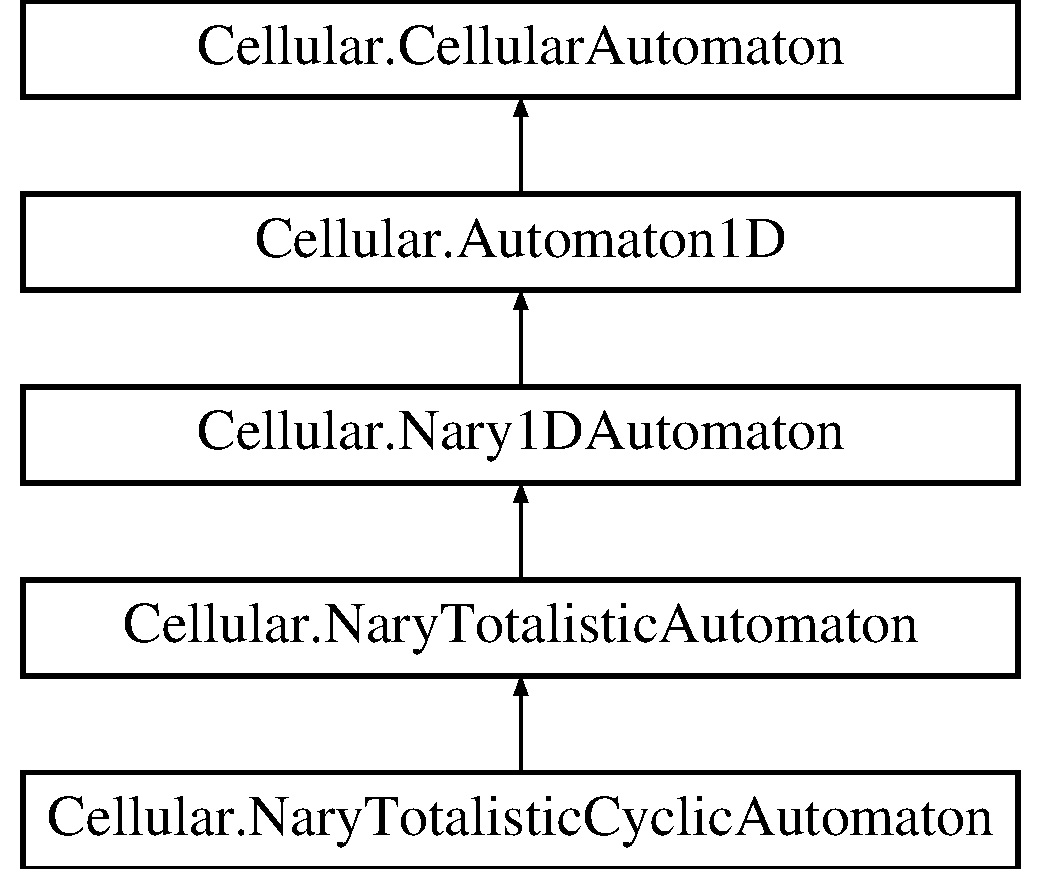
\includegraphics[height=5.000000cm]{class_cellular_1_1_nary_totalistic_cyclic_automaton}
\end{center}
\end{figure}
\subsection*{Public Member Functions}
\begin{DoxyCompactItemize}
\item 
\hyperlink{class_cellular_1_1_nary_totalistic_cyclic_automaton_a4616b10ffadcaef7a2d21b47976844af}{Nary\+Totalistic\+Cyclic\+Automaton} (int number\+Of\+States, int\mbox{[}$\,$\mbox{]} \hyperlink{class_cellular_1_1_nary_totalistic_automaton_a878c767c6823bd8ed8dc0f7d2ccb1fd2}{rule}, int\mbox{[}$\,$\mbox{]} initial\+State)
\item 
override object \hyperlink{class_cellular_1_1_nary_totalistic_cyclic_automaton_aa8d5a7d77a6dfc5f6e4fae6ba1c6cfd0}{Clone} ()
\begin{DoxyCompactList}\small\item\em Creates an appropriate copy of the C\+A. Its type and the specific rule are always preserved. However, the time (number of steps executed on the specific instance) is set back to 0. \end{DoxyCompactList}\item 
override string \hyperlink{class_cellular_1_1_nary_totalistic_cyclic_automaton_ac5c39cfb72386e3ab6132ab420091ae9}{Tell\+Type} ()
\begin{DoxyCompactList}\small\item\em Announces the runtime type of the C\+A including info about its rule. \end{DoxyCompactList}\end{DoxyCompactItemize}
\subsection*{Protected Member Functions}
\begin{DoxyCompactItemize}
\item 
override int \hyperlink{class_cellular_1_1_nary_totalistic_cyclic_automaton_a422dbcbd3e3cd3efdccc21724e7c6b01}{get\+Value\+At} (int index)
\begin{DoxyCompactList}\small\item\em This method simplifies boundary conditions. \end{DoxyCompactList}\end{DoxyCompactItemize}
\subsection*{Additional Inherited Members}


\subsection{Detailed Description}
Class representing any N-\/ary one-\/dimensional automaton with a totalistic rule -\/ cyclic variant. The new state of each cell depends on the sum of its current state and the current state of adjecent cells. 



Definition at line 7 of file Nary\+Totalistic\+Cyclic\+Automaton.\+cs.



\subsection{Constructor \& Destructor Documentation}
\hypertarget{class_cellular_1_1_nary_totalistic_cyclic_automaton_a4616b10ffadcaef7a2d21b47976844af}{}\index{Cellular\+::\+Nary\+Totalistic\+Cyclic\+Automaton@{Cellular\+::\+Nary\+Totalistic\+Cyclic\+Automaton}!Nary\+Totalistic\+Cyclic\+Automaton@{Nary\+Totalistic\+Cyclic\+Automaton}}
\index{Nary\+Totalistic\+Cyclic\+Automaton@{Nary\+Totalistic\+Cyclic\+Automaton}!Cellular\+::\+Nary\+Totalistic\+Cyclic\+Automaton@{Cellular\+::\+Nary\+Totalistic\+Cyclic\+Automaton}}
\subsubsection[{Nary\+Totalistic\+Cyclic\+Automaton(int number\+Of\+States, int[] rule, int[] initial\+State)}]{\setlength{\rightskip}{0pt plus 5cm}Cellular.\+Nary\+Totalistic\+Cyclic\+Automaton.\+Nary\+Totalistic\+Cyclic\+Automaton (
\begin{DoxyParamCaption}
\item[{int}]{number\+Of\+States, }
\item[{int\mbox{[}$\,$\mbox{]}}]{rule, }
\item[{int\mbox{[}$\,$\mbox{]}}]{initial\+State}
\end{DoxyParamCaption}
)}\label{class_cellular_1_1_nary_totalistic_cyclic_automaton_a4616b10ffadcaef7a2d21b47976844af}


Definition at line 9 of file Nary\+Totalistic\+Cyclic\+Automaton.\+cs.



\subsection{Member Function Documentation}
\hypertarget{class_cellular_1_1_nary_totalistic_cyclic_automaton_aa8d5a7d77a6dfc5f6e4fae6ba1c6cfd0}{}\index{Cellular\+::\+Nary\+Totalistic\+Cyclic\+Automaton@{Cellular\+::\+Nary\+Totalistic\+Cyclic\+Automaton}!Clone@{Clone}}
\index{Clone@{Clone}!Cellular\+::\+Nary\+Totalistic\+Cyclic\+Automaton@{Cellular\+::\+Nary\+Totalistic\+Cyclic\+Automaton}}
\subsubsection[{Clone()}]{\setlength{\rightskip}{0pt plus 5cm}override object Cellular.\+Nary\+Totalistic\+Cyclic\+Automaton.\+Clone (
\begin{DoxyParamCaption}
{}
\end{DoxyParamCaption}
)\hspace{0.3cm}{\ttfamily [virtual]}}\label{class_cellular_1_1_nary_totalistic_cyclic_automaton_aa8d5a7d77a6dfc5f6e4fae6ba1c6cfd0}


Creates an appropriate copy of the C\+A. Its type and the specific rule are always preserved. However, the time (number of steps executed on the specific instance) is set back to 0. 

\begin{DoxyReturn}{Returns}
A copy of the {\ttfamily \hyperlink{class_cellular_1_1_cellular_automaton}{Cellular\+Automaton}} as {\ttfamily System.\+Object}
\end{DoxyReturn}


Reimplemented from \hyperlink{class_cellular_1_1_nary_totalistic_automaton_a13f16113915ecec451fc4764a32044f9}{Cellular.\+Nary\+Totalistic\+Automaton}.



Definition at line 20 of file Nary\+Totalistic\+Cyclic\+Automaton.\+cs.

\hypertarget{class_cellular_1_1_nary_totalistic_cyclic_automaton_a422dbcbd3e3cd3efdccc21724e7c6b01}{}\index{Cellular\+::\+Nary\+Totalistic\+Cyclic\+Automaton@{Cellular\+::\+Nary\+Totalistic\+Cyclic\+Automaton}!get\+Value\+At@{get\+Value\+At}}
\index{get\+Value\+At@{get\+Value\+At}!Cellular\+::\+Nary\+Totalistic\+Cyclic\+Automaton@{Cellular\+::\+Nary\+Totalistic\+Cyclic\+Automaton}}
\subsubsection[{get\+Value\+At(int index)}]{\setlength{\rightskip}{0pt plus 5cm}override int Cellular.\+Nary\+Totalistic\+Cyclic\+Automaton.\+get\+Value\+At (
\begin{DoxyParamCaption}
\item[{int}]{index}
\end{DoxyParamCaption}
)\hspace{0.3cm}{\ttfamily [protected]}, {\ttfamily [virtual]}}\label{class_cellular_1_1_nary_totalistic_cyclic_automaton_a422dbcbd3e3cd3efdccc21724e7c6b01}


This method simplifies boundary conditions. 


\begin{DoxyParams}{Parameters}
{\em index} & Zero-\/based index (which value is required).\\
\hline
\end{DoxyParams}
\begin{DoxyReturn}{Returns}
Value from 0 to N-\/1.
\end{DoxyReturn}


Reimplemented from \hyperlink{class_cellular_1_1_nary1_d_automaton_adfd39915b66667efeeb9b16f154b9b6b}{Cellular.\+Nary1\+D\+Automaton}.



Definition at line 11 of file Nary\+Totalistic\+Cyclic\+Automaton.\+cs.

\hypertarget{class_cellular_1_1_nary_totalistic_cyclic_automaton_ac5c39cfb72386e3ab6132ab420091ae9}{}\index{Cellular\+::\+Nary\+Totalistic\+Cyclic\+Automaton@{Cellular\+::\+Nary\+Totalistic\+Cyclic\+Automaton}!Tell\+Type@{Tell\+Type}}
\index{Tell\+Type@{Tell\+Type}!Cellular\+::\+Nary\+Totalistic\+Cyclic\+Automaton@{Cellular\+::\+Nary\+Totalistic\+Cyclic\+Automaton}}
\subsubsection[{Tell\+Type()}]{\setlength{\rightskip}{0pt plus 5cm}override string Cellular.\+Nary\+Totalistic\+Cyclic\+Automaton.\+Tell\+Type (
\begin{DoxyParamCaption}
{}
\end{DoxyParamCaption}
)\hspace{0.3cm}{\ttfamily [virtual]}}\label{class_cellular_1_1_nary_totalistic_cyclic_automaton_ac5c39cfb72386e3ab6132ab420091ae9}


Announces the runtime type of the C\+A including info about its rule. 

\begin{DoxyReturn}{Returns}
Type of the C\+A as a string.
\end{DoxyReturn}


Reimplemented from \hyperlink{class_cellular_1_1_nary_totalistic_automaton_aa691c532a55638c7e3d0c125a4244773}{Cellular.\+Nary\+Totalistic\+Automaton}.



Definition at line 25 of file Nary\+Totalistic\+Cyclic\+Automaton.\+cs.



The documentation for this class was generated from the following file\+:\begin{DoxyCompactItemize}
\item 
C\+:/\+Martin/\+M\+F\+F/\+\_\+baka/\+Martin\+Dvorak/\+Cellular/\hyperlink{_nary_totalistic_cyclic_automaton_8cs}{Nary\+Totalistic\+Cyclic\+Automaton.\+cs}\end{DoxyCompactItemize}

\hypertarget{class_program}{}\section{Program Class Reference}
\label{class_program}\index{Program@{Program}}
\subsection*{Classes}
\begin{DoxyCompactItemize}
\item 
class \hyperlink{class_program_1_1_crypto_form}{Crypto\+Form}
\begin{DoxyCompactList}\small\item\em Windows application for users who want to encrypt their data using a cellular automata based algorithm. \end{DoxyCompactList}\item 
class \hyperlink{class_program_1_1_program}{Program}
\end{DoxyCompactItemize}
\subsection*{Static Public Attributes}
\begin{DoxyCompactItemize}
\item 
static Random \hyperlink{class_program_af2ace68664c9d781318def5ce37a7962}{rnd}
\end{DoxyCompactItemize}


\subsection{Detailed Description}


Definition at line 5 of file Program.\+cs.



\subsection{Member Data Documentation}
\hypertarget{class_program_af2ace68664c9d781318def5ce37a7962}{}\index{Program@{Program}!rnd@{rnd}}
\index{rnd@{rnd}!Program@{Program}}
\subsubsection[{rnd}]{\setlength{\rightskip}{0pt plus 5cm}Random Program.\+rnd\hspace{0.3cm}{\ttfamily [static]}}\label{class_program_af2ace68664c9d781318def5ce37a7962}


Definition at line 7 of file Program.\+cs.



The documentation for this class was generated from the following file\+:\begin{DoxyCompactItemize}
\item 
C\+:/\+Martin/\+M\+F\+F/\+\_\+baka/\+Martin\+Dvorak/\hyperlink{_martin_dvorak_2_program_8cs}{Program.\+cs}\end{DoxyCompactItemize}

\hypertarget{class_program_1_1_program}{}\section{Program.\+Program Class Reference}
\label{class_program_1_1_program}\index{Program.\+Program@{Program.\+Program}}


\subsection{Detailed Description}


Definition at line 6 of file Program.\+cs.



The documentation for this class was generated from the following file\+:\begin{DoxyCompactItemize}
\item 
C\+:/\+Martin/\+M\+F\+F/\+\_\+baka/\+Program/\hyperlink{_program_2_program_8cs}{Program.\+cs}\end{DoxyCompactItemize}

\hypertarget{class_crypto_1_1_randomness_testing}{}\section{Crypto.\+Randomness\+Testing Class Reference}
\label{class_crypto_1_1_randomness_testing}\index{Crypto.\+Randomness\+Testing@{Crypto.\+Randomness\+Testing}}


Static class that contains some tests of randomness for binary sequences.  


\subsection*{Static Public Member Functions}
\begin{DoxyCompactItemize}
\item 
static double \hyperlink{class_crypto_1_1_randomness_testing_a86ef256c8a7c87df3fdbbf5673465cb0}{Entropy\+Test} (Bit\+Array \hyperlink{jquery_8js_a2fa551895933fae935a0a6b87282241d}{b}, byte length\+Limit)
\begin{DoxyCompactList}\small\item\em Calculates the Shannon entropy of the Bit\+Array. \end{DoxyCompactList}\item 
static double \hyperlink{class_crypto_1_1_randomness_testing_af903b13649b40d4895243f51c62341cc}{Compression\+Test} (Bit\+Array \hyperlink{jquery_8js_a2fa551895933fae935a0a6b87282241d}{b})
\begin{DoxyCompactList}\small\item\em Tests how much the Bit\+Array can be compressed using gzip. \end{DoxyCompactList}\item 
static double \hyperlink{class_crypto_1_1_randomness_testing_a34e225189cd735e8cfa82f6ab3b7d97f}{Rate\+Sequence} (Bit\+Array sequence)
\end{DoxyCompactItemize}


\subsection{Detailed Description}
Static class that contains some tests of randomness for binary sequences. 



Definition at line 11 of file Randomness\+Testing.\+cs.



\subsection{Member Function Documentation}
\hypertarget{class_crypto_1_1_randomness_testing_af903b13649b40d4895243f51c62341cc}{}\index{Crypto\+::\+Randomness\+Testing@{Crypto\+::\+Randomness\+Testing}!Compression\+Test@{Compression\+Test}}
\index{Compression\+Test@{Compression\+Test}!Crypto\+::\+Randomness\+Testing@{Crypto\+::\+Randomness\+Testing}}
\subsubsection[{Compression\+Test(\+Bit\+Array b)}]{\setlength{\rightskip}{0pt plus 5cm}static double Crypto.\+Randomness\+Testing.\+Compression\+Test (
\begin{DoxyParamCaption}
\item[{Bit\+Array}]{b}
\end{DoxyParamCaption}
)\hspace{0.3cm}{\ttfamily [static]}}\label{class_crypto_1_1_randomness_testing_af903b13649b40d4895243f51c62341cc}


Tests how much the Bit\+Array can be compressed using gzip. 


\begin{DoxyParams}{Parameters}
{\em b} & Vector to rate.\\
\hline
\end{DoxyParams}
\begin{DoxyReturn}{Returns}
Ratio between new and old size.
\end{DoxyReturn}


Definition at line 69 of file Randomness\+Testing.\+cs.

\hypertarget{class_crypto_1_1_randomness_testing_a86ef256c8a7c87df3fdbbf5673465cb0}{}\index{Crypto\+::\+Randomness\+Testing@{Crypto\+::\+Randomness\+Testing}!Entropy\+Test@{Entropy\+Test}}
\index{Entropy\+Test@{Entropy\+Test}!Crypto\+::\+Randomness\+Testing@{Crypto\+::\+Randomness\+Testing}}
\subsubsection[{Entropy\+Test(\+Bit\+Array b, byte length\+Limit)}]{\setlength{\rightskip}{0pt plus 5cm}static double Crypto.\+Randomness\+Testing.\+Entropy\+Test (
\begin{DoxyParamCaption}
\item[{Bit\+Array}]{b, }
\item[{byte}]{length\+Limit}
\end{DoxyParamCaption}
)\hspace{0.3cm}{\ttfamily [static]}}\label{class_crypto_1_1_randomness_testing_a86ef256c8a7c87df3fdbbf5673465cb0}


Calculates the Shannon entropy of the Bit\+Array. 


\begin{DoxyParams}{Parameters}
{\em b} & Vector to rate.\\
\hline
{\em length\+Limit} & Blocks of size from 1 to {\ttfamily length\+Limit} will be counted.\\
\hline
\end{DoxyParams}
\begin{DoxyReturn}{Returns}
Number between 0 and 1. Only values very close to 1 are good.
\end{DoxyReturn}


Definition at line 19 of file Randomness\+Testing.\+cs.

\hypertarget{class_crypto_1_1_randomness_testing_a34e225189cd735e8cfa82f6ab3b7d97f}{}\index{Crypto\+::\+Randomness\+Testing@{Crypto\+::\+Randomness\+Testing}!Rate\+Sequence@{Rate\+Sequence}}
\index{Rate\+Sequence@{Rate\+Sequence}!Crypto\+::\+Randomness\+Testing@{Crypto\+::\+Randomness\+Testing}}
\subsubsection[{Rate\+Sequence(\+Bit\+Array sequence)}]{\setlength{\rightskip}{0pt plus 5cm}static double Crypto.\+Randomness\+Testing.\+Rate\+Sequence (
\begin{DoxyParamCaption}
\item[{Bit\+Array}]{sequence}
\end{DoxyParamCaption}
)\hspace{0.3cm}{\ttfamily [static]}}\label{class_crypto_1_1_randomness_testing_a34e225189cd735e8cfa82f6ab3b7d97f}


Definition at line 82 of file Randomness\+Testing.\+cs.



The documentation for this class was generated from the following file\+:\begin{DoxyCompactItemize}
\item 
C\+:/\+Martin/\+M\+F\+F/\+\_\+baka/\+Martin\+Dvorak/\+Crypto/\hyperlink{_randomness_testing_8cs}{Randomness\+Testing.\+cs}\end{DoxyCompactItemize}

\hypertarget{class_testing_1_1_random_test_test}{}\section{Testing.\+Random\+Test\+Test Class Reference}
\label{class_testing_1_1_random_test_test}\index{Testing.\+Random\+Test\+Test@{Testing.\+Random\+Test\+Test}}


Demonstration of the implemented tests of randomness, especially the entropy test.  


\subsection*{Static Public Member Functions}
\begin{DoxyCompactItemize}
\item 
static void \hyperlink{class_testing_1_1_random_test_test_ab90225a3e43ba2571ba730fc76c87a55}{Run\+Test} ()
\end{DoxyCompactItemize}


\subsection{Detailed Description}
Demonstration of the implemented tests of randomness, especially the entropy test. 



Definition at line 10 of file Random\+Test\+Test.\+cs.



\subsection{Member Function Documentation}
\hypertarget{class_testing_1_1_random_test_test_ab90225a3e43ba2571ba730fc76c87a55}{}\index{Testing\+::\+Random\+Test\+Test@{Testing\+::\+Random\+Test\+Test}!Run\+Test@{Run\+Test}}
\index{Run\+Test@{Run\+Test}!Testing\+::\+Random\+Test\+Test@{Testing\+::\+Random\+Test\+Test}}
\subsubsection[{Run\+Test()}]{\setlength{\rightskip}{0pt plus 5cm}static void Testing.\+Random\+Test\+Test.\+Run\+Test (
\begin{DoxyParamCaption}
{}
\end{DoxyParamCaption}
)\hspace{0.3cm}{\ttfamily [static]}}\label{class_testing_1_1_random_test_test_ab90225a3e43ba2571ba730fc76c87a55}


Definition at line 22 of file Random\+Test\+Test.\+cs.



The documentation for this class was generated from the following file\+:\begin{DoxyCompactItemize}
\item 
C\+:/\+Martin/\+M\+F\+F/\+\_\+baka/\+Martin\+Dvorak/\+Testing/\hyperlink{_random_test_test_8cs}{Random\+Test\+Test.\+cs}\end{DoxyCompactItemize}

\hypertarget{class_testing_1_1_search_longest}{}\section{Testing.\+Search\+Longest Class Reference}
\label{class_testing_1_1_search_longest}\index{Testing.\+Search\+Longest@{Testing.\+Search\+Longest}}


Simple demonstration of working with period lengths.  


\subsection*{Static Public Member Functions}
\begin{DoxyCompactItemize}
\item 
static long \hyperlink{class_testing_1_1_search_longest_ab0c6b6cb67d56bd5d739b41bd71590ee}{Longest\+Period} ()
\begin{DoxyCompactList}\small\item\em Searches for a C\+A with the longest period on some sample data. \end{DoxyCompactList}\end{DoxyCompactItemize}


\subsection{Detailed Description}
Simple demonstration of working with period lengths. 



Definition at line 11 of file Search\+Longest.\+cs.



\subsection{Member Function Documentation}
\hypertarget{class_testing_1_1_search_longest_ab0c6b6cb67d56bd5d739b41bd71590ee}{}\index{Testing\+::\+Search\+Longest@{Testing\+::\+Search\+Longest}!Longest\+Period@{Longest\+Period}}
\index{Longest\+Period@{Longest\+Period}!Testing\+::\+Search\+Longest@{Testing\+::\+Search\+Longest}}
\subsubsection[{Longest\+Period()}]{\setlength{\rightskip}{0pt plus 5cm}static long Testing.\+Search\+Longest.\+Longest\+Period (
\begin{DoxyParamCaption}
{}
\end{DoxyParamCaption}
)\hspace{0.3cm}{\ttfamily [static]}}\label{class_testing_1_1_search_longest_ab0c6b6cb67d56bd5d739b41bd71590ee}


Searches for a C\+A with the longest period on some sample data. 

\begin{DoxyReturn}{Returns}
The longest period.
\end{DoxyReturn}


Definition at line 40 of file Search\+Longest.\+cs.



The documentation for this class was generated from the following file\+:\begin{DoxyCompactItemize}
\item 
C\+:/\+Martin/\+M\+F\+F/\+\_\+baka/\+Martin\+Dvorak/\+Testing/\hyperlink{_search_longest_8cs}{Search\+Longest.\+cs}\end{DoxyCompactItemize}

\hypertarget{class_crypto_1_1_search_s_g_a}{}\section{Crypto.\+Search\+S\+G\+A Class Reference}
\label{class_crypto_1_1_search_s_g_a}\index{Crypto.\+Search\+S\+G\+A@{Crypto.\+Search\+S\+G\+A}}


Static class that can be used to pre-\/generate good key extenders for the genetic algorithm.  


\subsection*{Static Public Member Functions}
\begin{DoxyCompactItemize}
\item 
static void \hyperlink{class_crypto_1_1_search_s_g_a_a5c735e0bfccfc7d2fb91fd772be42ae7}{Search\+For\+Good\+Extenders} ()
\begin{DoxyCompactList}\small\item\em Infinite loop of \hyperlink{class_crypto_1_1_key_extender_genetic}{Key\+Extender\+Genetic} for collecting data about good key extending primitives. Generates text output into the same directory. \end{DoxyCompactList}\end{DoxyCompactItemize}


\subsection{Detailed Description}
Static class that can be used to pre-\/generate good key extenders for the genetic algorithm. 



Definition at line 11 of file Search\+S\+G\+A.\+cs.



\subsection{Member Function Documentation}
\hypertarget{class_crypto_1_1_search_s_g_a_a5c735e0bfccfc7d2fb91fd772be42ae7}{}\index{Crypto\+::\+Search\+S\+G\+A@{Crypto\+::\+Search\+S\+G\+A}!Search\+For\+Good\+Extenders@{Search\+For\+Good\+Extenders}}
\index{Search\+For\+Good\+Extenders@{Search\+For\+Good\+Extenders}!Crypto\+::\+Search\+S\+G\+A@{Crypto\+::\+Search\+S\+G\+A}}
\subsubsection[{Search\+For\+Good\+Extenders()}]{\setlength{\rightskip}{0pt plus 5cm}static void Crypto.\+Search\+S\+G\+A.\+Search\+For\+Good\+Extenders (
\begin{DoxyParamCaption}
{}
\end{DoxyParamCaption}
)\hspace{0.3cm}{\ttfamily [static]}}\label{class_crypto_1_1_search_s_g_a_a5c735e0bfccfc7d2fb91fd772be42ae7}


Infinite loop of \hyperlink{class_crypto_1_1_key_extender_genetic}{Key\+Extender\+Genetic} for collecting data about good key extending primitives. Generates text output into the same directory. 



Definition at line 17 of file Search\+S\+G\+A.\+cs.



The documentation for this class was generated from the following file\+:\begin{DoxyCompactItemize}
\item 
C\+:/\+Martin/\+M\+F\+F/\+\_\+baka/\+Martin\+Dvorak/\+Crypto/\hyperlink{_search_s_g_a_8cs}{Search\+S\+G\+A.\+cs}\end{DoxyCompactItemize}

\hypertarget{class_cellular_1_1_totalistic2_d_automaton}{}\section{Cellular.\+Totalistic2\+D\+Automaton Class Reference}
\label{class_cellular_1_1_totalistic2_d_automaton}\index{Cellular.\+Totalistic2\+D\+Automaton@{Cellular.\+Totalistic2\+D\+Automaton}}


Class representing a totalistic 2\+D automaton that uses Moore Neighborhood.  


Inheritance diagram for Cellular.\+Totalistic2\+D\+Automaton\+:\begin{figure}[H]
\begin{center}
\leavevmode
\includegraphics[height=6.000000cm]{class_cellular_1_1_totalistic2_d_automaton}
\end{center}
\end{figure}
\subsection*{Public Member Functions}
\begin{DoxyCompactItemize}
\item 
\hyperlink{class_cellular_1_1_totalistic2_d_automaton_a0a2cfd3f0c13cae481d0278630c71a0e}{Totalistic2\+D\+Automaton} (bool\mbox{[}$\,$\mbox{]} \hyperlink{class_cellular_1_1_totalistic2_d_automaton_a4752e3402c58243f7f342e21ddad3b05}{rule\+Live}, bool\mbox{[}$\,$\mbox{]} rule\+Dead, int \hyperlink{class_cellular_1_1_automaton2_d_a1e9e5ec637c747a859c346839c90d174}{width}, int height, Random rnd)
\begin{DoxyCompactList}\small\item\em Creates a new totalistic 2\+D automaton of given ruleset with given initial state. \end{DoxyCompactList}\item 
\hyperlink{class_cellular_1_1_totalistic2_d_automaton_a3a58155945c0ef836c06e5a568afe1a0}{Totalistic2\+D\+Automaton} (bool\mbox{[}$\,$\mbox{]} \hyperlink{class_cellular_1_1_totalistic2_d_automaton_a4752e3402c58243f7f342e21ddad3b05}{rule\+Live}, bool\mbox{[}$\,$\mbox{]} rule\+Dead, Bit\+Array\mbox{[}$\,$\mbox{]} initial\+State)
\begin{DoxyCompactList}\small\item\em Creates a new totalistic 2\+D automaton of given ruleset with given initial state. \end{DoxyCompactList}\item 
override void \hyperlink{class_cellular_1_1_totalistic2_d_automaton_a7f85cac5420f67a936cbd4cef33c4abc}{Step} ()
\begin{DoxyCompactList}\small\item\em Performs one step of the cellular automaton. Always calls \end{DoxyCompactList}\item 
override object \hyperlink{class_cellular_1_1_totalistic2_d_automaton_ae78cf4c3f8245adf64ec9a173330804f}{Clone} ()
\begin{DoxyCompactList}\small\item\em Creates an appropriate copy of the C\+A. Its type and the specific rule are always preserved. However, the time (number of steps executed on the specific instance) is set back to 0. \end{DoxyCompactList}\item 
override string \hyperlink{class_cellular_1_1_totalistic2_d_automaton_aa009c674cd109fa70173e9893f6d3b09}{Tell\+Type} ()
\begin{DoxyCompactList}\small\item\em Announces the runtime type of the C\+A including info about its rule. It serves for debugging purposes. \end{DoxyCompactList}\end{DoxyCompactItemize}
\subsection*{Protected Member Functions}
\begin{DoxyCompactItemize}
\item 
override \hyperlink{interface_cellular_1_1_i_binary_c_a}{I\+Binary\+C\+A} \hyperlink{class_cellular_1_1_totalistic2_d_automaton_ad5cc3f46a556aa1b1c99bdfa92f5ba1d}{clone\+Template} (Bit\+Array\mbox{[}$\,$\mbox{]} new\+Instance\+State)
\end{DoxyCompactItemize}
\subsection*{Protected Attributes}
\begin{DoxyCompactItemize}
\item 
bool\mbox{[}$\,$\mbox{]} \hyperlink{class_cellular_1_1_totalistic2_d_automaton_a4752e3402c58243f7f342e21ddad3b05}{rule\+Live}
\end{DoxyCompactItemize}


\subsection{Detailed Description}
Class representing a totalistic 2\+D automaton that uses Moore Neighborhood. 



Definition at line 9 of file Totalistic2\+D\+Automaton.\+cs.



\subsection{Constructor \& Destructor Documentation}
\hypertarget{class_cellular_1_1_totalistic2_d_automaton_a0a2cfd3f0c13cae481d0278630c71a0e}{}\index{Cellular\+::\+Totalistic2\+D\+Automaton@{Cellular\+::\+Totalistic2\+D\+Automaton}!Totalistic2\+D\+Automaton@{Totalistic2\+D\+Automaton}}
\index{Totalistic2\+D\+Automaton@{Totalistic2\+D\+Automaton}!Cellular\+::\+Totalistic2\+D\+Automaton@{Cellular\+::\+Totalistic2\+D\+Automaton}}
\subsubsection[{Totalistic2\+D\+Automaton(bool[] rule\+Live, bool[] rule\+Dead, int width, int height, Random rnd)}]{\setlength{\rightskip}{0pt plus 5cm}Cellular.\+Totalistic2\+D\+Automaton.\+Totalistic2\+D\+Automaton (
\begin{DoxyParamCaption}
\item[{bool\mbox{[}$\,$\mbox{]}}]{rule\+Live, }
\item[{bool\mbox{[}$\,$\mbox{]}}]{rule\+Dead, }
\item[{int}]{width, }
\item[{int}]{height, }
\item[{Random}]{rnd}
\end{DoxyParamCaption}
)}\label{class_cellular_1_1_totalistic2_d_automaton_a0a2cfd3f0c13cae481d0278630c71a0e}


Creates a new totalistic 2\+D automaton of given ruleset with given initial state. 


\begin{DoxyParams}{Parameters}
{\em rule\+Live} & Array that must contain 9 logical values. The value in {\ttfamily rule\+Live\mbox{[}i\mbox{]}} says what happens to a living cell when it has exactly i neighbours alive.\\
\hline
{\em rule\+Dead} & Array that must contain 9 logical values. The value in {\ttfamily rule\+Dead\mbox{[}i\mbox{]}} says what happens to a dead cell when it has exactly i neighbours alive.\\
\hline
{\em width} & The width of the new C\+A (length of rows).\\
\hline
{\em height} & The height of the new C\+A (number of rows).\\
\hline
{\em rnd} & Pseudo\+R\+N\+G instance that will be used to generate the original state.\\
\hline
\end{DoxyParams}


Definition at line 23 of file Totalistic2\+D\+Automaton.\+cs.

\hypertarget{class_cellular_1_1_totalistic2_d_automaton_a3a58155945c0ef836c06e5a568afe1a0}{}\index{Cellular\+::\+Totalistic2\+D\+Automaton@{Cellular\+::\+Totalistic2\+D\+Automaton}!Totalistic2\+D\+Automaton@{Totalistic2\+D\+Automaton}}
\index{Totalistic2\+D\+Automaton@{Totalistic2\+D\+Automaton}!Cellular\+::\+Totalistic2\+D\+Automaton@{Cellular\+::\+Totalistic2\+D\+Automaton}}
\subsubsection[{Totalistic2\+D\+Automaton(bool[] rule\+Live, bool[] rule\+Dead, Bit\+Array[] initial\+State)}]{\setlength{\rightskip}{0pt plus 5cm}Cellular.\+Totalistic2\+D\+Automaton.\+Totalistic2\+D\+Automaton (
\begin{DoxyParamCaption}
\item[{bool\mbox{[}$\,$\mbox{]}}]{rule\+Live, }
\item[{bool\mbox{[}$\,$\mbox{]}}]{rule\+Dead, }
\item[{Bit\+Array\mbox{[}$\,$\mbox{]}}]{initial\+State}
\end{DoxyParamCaption}
)}\label{class_cellular_1_1_totalistic2_d_automaton_a3a58155945c0ef836c06e5a568afe1a0}


Creates a new totalistic 2\+D automaton of given ruleset with given initial state. 


\begin{DoxyParams}{Parameters}
{\em rule\+Live} & Array that must contain 9 logical values. The value in {\ttfamily rule\+Live\mbox{[}i\mbox{]}} says what happens to a living cell when it has exactly i neighbours alive.\\
\hline
{\em rule\+Dead} & Array that must contain 9 logical values. The value in {\ttfamily rule\+Dead\mbox{[}i\mbox{]}} says what happens to a dead cell when it has exactly i neighbours alive.\\
\hline
{\em initial\+State} & An array of {\ttfamily Bit\+Array}s describing the initial state of the C\+A. This also determines the size (width, height) of the new C\+A.\\
\hline
\end{DoxyParams}


Definition at line 37 of file Totalistic2\+D\+Automaton.\+cs.



\subsection{Member Function Documentation}
\hypertarget{class_cellular_1_1_totalistic2_d_automaton_ae78cf4c3f8245adf64ec9a173330804f}{}\index{Cellular\+::\+Totalistic2\+D\+Automaton@{Cellular\+::\+Totalistic2\+D\+Automaton}!Clone@{Clone}}
\index{Clone@{Clone}!Cellular\+::\+Totalistic2\+D\+Automaton@{Cellular\+::\+Totalistic2\+D\+Automaton}}
\subsubsection[{Clone()}]{\setlength{\rightskip}{0pt plus 5cm}override object Cellular.\+Totalistic2\+D\+Automaton.\+Clone (
\begin{DoxyParamCaption}
{}
\end{DoxyParamCaption}
)\hspace{0.3cm}{\ttfamily [virtual]}}\label{class_cellular_1_1_totalistic2_d_automaton_ae78cf4c3f8245adf64ec9a173330804f}


Creates an appropriate copy of the C\+A. Its type and the specific rule are always preserved. However, the time (number of steps executed on the specific instance) is set back to 0. 

\begin{DoxyReturn}{Returns}
A copy of the {\ttfamily \hyperlink{class_cellular_1_1_cellular_automaton}{Cellular\+Automaton}} as an {\ttfamily Object}
\end{DoxyReturn}


Implements \hyperlink{class_cellular_1_1_cellular_automaton_affd487b397cdbbbb1982815bbcd8e7d3}{Cellular.\+Cellular\+Automaton}.



Definition at line 202 of file Totalistic2\+D\+Automaton.\+cs.

\hypertarget{class_cellular_1_1_totalistic2_d_automaton_ad5cc3f46a556aa1b1c99bdfa92f5ba1d}{}\index{Cellular\+::\+Totalistic2\+D\+Automaton@{Cellular\+::\+Totalistic2\+D\+Automaton}!clone\+Template@{clone\+Template}}
\index{clone\+Template@{clone\+Template}!Cellular\+::\+Totalistic2\+D\+Automaton@{Cellular\+::\+Totalistic2\+D\+Automaton}}
\subsubsection[{clone\+Template(\+Bit\+Array[] new\+Instance\+State)}]{\setlength{\rightskip}{0pt plus 5cm}override {\bf I\+Binary\+C\+A} Cellular.\+Totalistic2\+D\+Automaton.\+clone\+Template (
\begin{DoxyParamCaption}
\item[{Bit\+Array\mbox{[}$\,$\mbox{]}}]{new\+Instance\+State}
\end{DoxyParamCaption}
)\hspace{0.3cm}{\ttfamily [protected]}, {\ttfamily [virtual]}}\label{class_cellular_1_1_totalistic2_d_automaton_ad5cc3f46a556aa1b1c99bdfa92f5ba1d}


Implements \hyperlink{class_cellular_1_1_binary2_d_automaton_ad2d31668c7b8f8e959575e03b995273f}{Cellular.\+Binary2\+D\+Automaton}.



Definition at line 207 of file Totalistic2\+D\+Automaton.\+cs.

\hypertarget{class_cellular_1_1_totalistic2_d_automaton_a7f85cac5420f67a936cbd4cef33c4abc}{}\index{Cellular\+::\+Totalistic2\+D\+Automaton@{Cellular\+::\+Totalistic2\+D\+Automaton}!Step@{Step}}
\index{Step@{Step}!Cellular\+::\+Totalistic2\+D\+Automaton@{Cellular\+::\+Totalistic2\+D\+Automaton}}
\subsubsection[{Step()}]{\setlength{\rightskip}{0pt plus 5cm}override void Cellular.\+Totalistic2\+D\+Automaton.\+Step (
\begin{DoxyParamCaption}
{}
\end{DoxyParamCaption}
)}\label{class_cellular_1_1_totalistic2_d_automaton_a7f85cac5420f67a936cbd4cef33c4abc}


Performs one step of the cellular automaton. Always calls 

{\ttfamily \hyperlink{class_cellular_1_1_cellular_automaton_aa70848d58015575974bc875ac5a89ae7}{Cellular\+Automaton.\+Step()};}. 

Implements \hyperlink{interface_cellular_1_1_i_binary_c_a_a6a04c7374538c49df07efa176e0dd3c3}{Cellular.\+I\+Binary\+C\+A}.



Definition at line 52 of file Totalistic2\+D\+Automaton.\+cs.

\hypertarget{class_cellular_1_1_totalistic2_d_automaton_aa009c674cd109fa70173e9893f6d3b09}{}\index{Cellular\+::\+Totalistic2\+D\+Automaton@{Cellular\+::\+Totalistic2\+D\+Automaton}!Tell\+Type@{Tell\+Type}}
\index{Tell\+Type@{Tell\+Type}!Cellular\+::\+Totalistic2\+D\+Automaton@{Cellular\+::\+Totalistic2\+D\+Automaton}}
\subsubsection[{Tell\+Type()}]{\setlength{\rightskip}{0pt plus 5cm}override string Cellular.\+Totalistic2\+D\+Automaton.\+Tell\+Type (
\begin{DoxyParamCaption}
{}
\end{DoxyParamCaption}
)}\label{class_cellular_1_1_totalistic2_d_automaton_aa009c674cd109fa70173e9893f6d3b09}


Announces the runtime type of the C\+A including info about its rule. It serves for debugging purposes. 

\begin{DoxyReturn}{Returns}
The same string as calling 
\begin{DoxyCode}
CellularAutomaton.TellType();
\end{DoxyCode}
.
\end{DoxyReturn}


Implements \hyperlink{interface_cellular_1_1_i_binary_c_a_aa67feabf5d1513aa74076d255c661948}{Cellular.\+I\+Binary\+C\+A}.



Definition at line 212 of file Totalistic2\+D\+Automaton.\+cs.



\subsection{Member Data Documentation}
\hypertarget{class_cellular_1_1_totalistic2_d_automaton_a4752e3402c58243f7f342e21ddad3b05}{}\index{Cellular\+::\+Totalistic2\+D\+Automaton@{Cellular\+::\+Totalistic2\+D\+Automaton}!rule\+Live@{rule\+Live}}
\index{rule\+Live@{rule\+Live}!Cellular\+::\+Totalistic2\+D\+Automaton@{Cellular\+::\+Totalistic2\+D\+Automaton}}
\subsubsection[{rule\+Live}]{\setlength{\rightskip}{0pt plus 5cm}bool \mbox{[}$\,$\mbox{]} Cellular.\+Totalistic2\+D\+Automaton.\+rule\+Live\hspace{0.3cm}{\ttfamily [protected]}}\label{class_cellular_1_1_totalistic2_d_automaton_a4752e3402c58243f7f342e21ddad3b05}


Definition at line 11 of file Totalistic2\+D\+Automaton.\+cs.



The documentation for this class was generated from the following file\+:\begin{DoxyCompactItemize}
\item 
C\+:/\+Martin/\+M\+F\+F/\+\_\+baka/\+Martin\+Dvorak/\+Cellular/\hyperlink{_totalistic2_d_automaton_8cs}{Totalistic2\+D\+Automaton.\+cs}\end{DoxyCompactItemize}

\hypertarget{class_testing_1_1_totalistic_ternary_test}{}\section{Testing.\+Totalistic\+Ternary\+Test Class Reference}
\label{class_testing_1_1_totalistic_ternary_test}\index{Testing.\+Totalistic\+Ternary\+Test@{Testing.\+Totalistic\+Ternary\+Test}}


Simple demonstration of 1\+D ternary totalistic automata.  


\subsection*{Static Public Member Functions}
\begin{DoxyCompactItemize}
\item 
static void \hyperlink{class_testing_1_1_totalistic_ternary_test_a3ba8f77c71da1744625f2e3714dd9c1f}{Run\+Test} ()
\end{DoxyCompactItemize}


\subsection{Detailed Description}
Simple demonstration of 1\+D ternary totalistic automata. 



Definition at line 9 of file Totalistic\+Ternary\+Test.\+cs.



\subsection{Member Function Documentation}
\hypertarget{class_testing_1_1_totalistic_ternary_test_a3ba8f77c71da1744625f2e3714dd9c1f}{}\index{Testing\+::\+Totalistic\+Ternary\+Test@{Testing\+::\+Totalistic\+Ternary\+Test}!Run\+Test@{Run\+Test}}
\index{Run\+Test@{Run\+Test}!Testing\+::\+Totalistic\+Ternary\+Test@{Testing\+::\+Totalistic\+Ternary\+Test}}
\subsubsection[{Run\+Test()}]{\setlength{\rightskip}{0pt plus 5cm}static void Testing.\+Totalistic\+Ternary\+Test.\+Run\+Test (
\begin{DoxyParamCaption}
{}
\end{DoxyParamCaption}
)\hspace{0.3cm}{\ttfamily [static]}}\label{class_testing_1_1_totalistic_ternary_test_a3ba8f77c71da1744625f2e3714dd9c1f}


Definition at line 11 of file Totalistic\+Ternary\+Test.\+cs.



The documentation for this class was generated from the following file\+:\begin{DoxyCompactItemize}
\item 
C\+:/\+Martin/\+M\+F\+F/\+\_\+baka/\+Martin\+Dvorak/\+Testing/\hyperlink{_totalistic_ternary_test_8cs}{Totalistic\+Ternary\+Test.\+cs}\end{DoxyCompactItemize}

\hypertarget{class_cellular_1_1_utilities}{}\section{Cellular.\+Utilities Class Reference}
\label{class_cellular_1_1_utilities}\index{Cellular.\+Utilities@{Cellular.\+Utilities}}


Static class packing a group of utilities for working with C\+A.  


\subsection*{Classes}
\begin{DoxyCompactItemize}
\item 
class \hyperlink{class_cellular_1_1_utilities_1_1_all_binary_sequences}{All\+Binary\+Sequences}
\begin{DoxyCompactList}\small\item\em Class for enumerating all binary sequences of a given length. Starting from 00...00, ending at 11...11. \end{DoxyCompactList}\end{DoxyCompactItemize}
\subsection*{Static Public Member Functions}
\begin{DoxyCompactItemize}
\item 
static bool\mbox{[}$\,$\mbox{]} \hyperlink{class_cellular_1_1_utilities_a6f1fcc096938174c779453fb588cbfdb}{Uint\+Arr\+To\+Bool\+Arr} (uint\mbox{[}$\,$\mbox{]} input)
\begin{DoxyCompactList}\small\item\em Converts an array of {\ttfamily System.\+U\+Int32} into an array of {\ttfamily System.\+Boolean}. The input is treated as M\+S\+B-\/first. \end{DoxyCompactList}\item 
static Bit\+Array \hyperlink{class_cellular_1_1_utilities_a3e6d6ebde1b445f03d3c0b1a9c0274e6}{Uint\+Arr\+To\+Bit\+Arr} (uint\mbox{[}$\,$\mbox{]} input)
\begin{DoxyCompactList}\small\item\em Converts an array of {\ttfamily System.\+U\+Int32} into an array of {\ttfamily System.\+Collections.\+Bit\+Array}. The input is treated as M\+S\+B-\/first. \end{DoxyCompactList}\item 
static bool\mbox{[}$\,$\mbox{]} \hyperlink{class_cellular_1_1_utilities_a1c47a345afd4e991876f6ae6c4723591}{Bit\+Arr\+To\+Bool\+Arr} (Bit\+Array bit\+Array)
\item 
static long \hyperlink{class_cellular_1_1_utilities_a8ebd90cf7f8d6ce2235d26f9feeddfae}{Period\+Length\+Fast} (\hyperlink{class_cellular_1_1_cellular_automaton}{Cellular\+Automaton} C\+A, long limit, out long time)
\begin{DoxyCompactList}\small\item\em Calculates a period (number of steps between repetitions) of a C\+A. This method is fast, but unreliable! It gives only the lower estimate (because of hashing). \end{DoxyCompactList}\item 
static long \hyperlink{class_cellular_1_1_utilities_a7a43545f264bf30884c8486a14fb4f43}{Period\+Length\+Fast} (\hyperlink{class_cellular_1_1_cellular_automaton}{Cellular\+Automaton} C\+A)
\begin{DoxyCompactList}\small\item\em Calculates a period (number of steps between repetitions) of a C\+A. This method is fast, but unreliable! It gives only the lower estimate (because of hashing). \end{DoxyCompactList}\item 
static long \hyperlink{class_cellular_1_1_utilities_aa0b71d2f39b127f7078a35263adbfd55}{Period\+Length\+Slow} (\hyperlink{interface_cellular_1_1_i_binary_c_a}{I\+Binary\+C\+A} C\+A, long limit, out long time)
\begin{DoxyCompactList}\small\item\em Calculates a period (number of steps between repetitions) of a binary C\+A. This method is slower, but reliable. \end{DoxyCompactList}\item 
static bool\mbox{[}$\,$\mbox{]} \hyperlink{class_cellular_1_1_utilities_a3f20fa274e0db626d4052fe233f7a00f}{Random\+Bool\+Arr} (int length, Random rnd)
\begin{DoxyCompactList}\small\item\em Generates a random array of {\ttfamily System.\+Boolean} of given length. \end{DoxyCompactList}\item 
static bool\mbox{[}$\,$\mbox{]} \hyperlink{class_cellular_1_1_utilities_a069e9224bbd6f305d17e38d6290424cd}{Random\+Bool\+Arr} (int length)
\begin{DoxyCompactList}\small\item\em Generates a random array of {\ttfamily System.\+Boolean} of given length. The instance of Pseudo-\/random number generator is created locally, so this method is unsuitable for repeated use. \end{DoxyCompactList}\item 
static Bit\+Array \hyperlink{class_cellular_1_1_utilities_a887bbf207bece7f1bfa93d3d3fab547d}{Random\+Bit\+Arr} (int length, Random rnd)
\begin{DoxyCompactList}\small\item\em Generates a random array of {\ttfamily System.\+Collections.\+Bit\+Array} of given length. \end{DoxyCompactList}\item 
static Bit\+Array \hyperlink{class_cellular_1_1_utilities_a9cf5e2901915830e230c8affacfcec18}{Random\+Bit\+Arr} (int length)
\begin{DoxyCompactList}\small\item\em Generates a random array of {\ttfamily System.\+Collections.\+Bit\+Array} of given length. The instance of Pseudo-\/random number generator is created locally, so this method is unsuitable for repeated use. \end{DoxyCompactList}\end{DoxyCompactItemize}


\subsection{Detailed Description}
Static class packing a group of utilities for working with C\+A. 



Definition at line 11 of file Utilities.\+cs.



\subsection{Member Function Documentation}
\hypertarget{class_cellular_1_1_utilities_a1c47a345afd4e991876f6ae6c4723591}{}\index{Cellular\+::\+Utilities@{Cellular\+::\+Utilities}!Bit\+Arr\+To\+Bool\+Arr@{Bit\+Arr\+To\+Bool\+Arr}}
\index{Bit\+Arr\+To\+Bool\+Arr@{Bit\+Arr\+To\+Bool\+Arr}!Cellular\+::\+Utilities@{Cellular\+::\+Utilities}}
\subsubsection[{Bit\+Arr\+To\+Bool\+Arr(\+Bit\+Array bit\+Array)}]{\setlength{\rightskip}{0pt plus 5cm}static bool \mbox{[}$\,$\mbox{]} Cellular.\+Utilities.\+Bit\+Arr\+To\+Bool\+Arr (
\begin{DoxyParamCaption}
\item[{Bit\+Array}]{bit\+Array}
\end{DoxyParamCaption}
)\hspace{0.3cm}{\ttfamily [static]}}\label{class_cellular_1_1_utilities_a1c47a345afd4e991876f6ae6c4723591}


Definition at line 59 of file Utilities.\+cs.

\hypertarget{class_cellular_1_1_utilities_a8ebd90cf7f8d6ce2235d26f9feeddfae}{}\index{Cellular\+::\+Utilities@{Cellular\+::\+Utilities}!Period\+Length\+Fast@{Period\+Length\+Fast}}
\index{Period\+Length\+Fast@{Period\+Length\+Fast}!Cellular\+::\+Utilities@{Cellular\+::\+Utilities}}
\subsubsection[{Period\+Length\+Fast(\+Cellular\+Automaton C\+A, long limit, out long time)}]{\setlength{\rightskip}{0pt plus 5cm}static long Cellular.\+Utilities.\+Period\+Length\+Fast (
\begin{DoxyParamCaption}
\item[{{\bf Cellular\+Automaton}}]{C\+A, }
\item[{long}]{limit, }
\item[{out long}]{time}
\end{DoxyParamCaption}
)\hspace{0.3cm}{\ttfamily [static]}}\label{class_cellular_1_1_utilities_a8ebd90cf7f8d6ce2235d26f9feeddfae}


Calculates a period (number of steps between repetitions) of a C\+A. This method is fast, but unreliable! It gives only the lower estimate (because of hashing). 


\begin{DoxyParams}{Parameters}
{\em C\+A} & The examined cellular automaton. Don\textquotesingle{}t worry, this method won\textquotesingle{}t modify it.\\
\hline
{\em limit} & Number of steps that will be performed in no repetition is found earlier.\\
\hline
{\em time} & Output parameter telling the time of a first repetition (second occurence of the same state). It is the number of steps done since calling this method (not a real time, not a period length).\\
\hline
\end{DoxyParams}
\begin{DoxyReturn}{Returns}
If a period is found within the limit, it returns the length of the period. Otherwise, it returns -\/1.
\end{DoxyReturn}


Definition at line 79 of file Utilities.\+cs.

\hypertarget{class_cellular_1_1_utilities_a7a43545f264bf30884c8486a14fb4f43}{}\index{Cellular\+::\+Utilities@{Cellular\+::\+Utilities}!Period\+Length\+Fast@{Period\+Length\+Fast}}
\index{Period\+Length\+Fast@{Period\+Length\+Fast}!Cellular\+::\+Utilities@{Cellular\+::\+Utilities}}
\subsubsection[{Period\+Length\+Fast(\+Cellular\+Automaton C\+A)}]{\setlength{\rightskip}{0pt plus 5cm}static long Cellular.\+Utilities.\+Period\+Length\+Fast (
\begin{DoxyParamCaption}
\item[{{\bf Cellular\+Automaton}}]{C\+A}
\end{DoxyParamCaption}
)\hspace{0.3cm}{\ttfamily [static]}}\label{class_cellular_1_1_utilities_a7a43545f264bf30884c8486a14fb4f43}


Calculates a period (number of steps between repetitions) of a C\+A. This method is fast, but unreliable! It gives only the lower estimate (because of hashing). 


\begin{DoxyParams}{Parameters}
{\em C\+A} & The examined cellular automaton. Don\textquotesingle{}t worry, this method won\textquotesingle{}t modify it.\\
\hline
\end{DoxyParams}
\begin{DoxyReturn}{Returns}
If a period is found within 2$^\wedge$30 steps, it returns the length of the period. Otherwise, it returns -\/1.
\end{DoxyReturn}


Definition at line 106 of file Utilities.\+cs.

\hypertarget{class_cellular_1_1_utilities_aa0b71d2f39b127f7078a35263adbfd55}{}\index{Cellular\+::\+Utilities@{Cellular\+::\+Utilities}!Period\+Length\+Slow@{Period\+Length\+Slow}}
\index{Period\+Length\+Slow@{Period\+Length\+Slow}!Cellular\+::\+Utilities@{Cellular\+::\+Utilities}}
\subsubsection[{Period\+Length\+Slow(\+I\+Binary\+C\+A C\+A, long limit, out long time)}]{\setlength{\rightskip}{0pt plus 5cm}static long Cellular.\+Utilities.\+Period\+Length\+Slow (
\begin{DoxyParamCaption}
\item[{{\bf I\+Binary\+C\+A}}]{C\+A, }
\item[{long}]{limit, }
\item[{out long}]{time}
\end{DoxyParamCaption}
)\hspace{0.3cm}{\ttfamily [static]}}\label{class_cellular_1_1_utilities_aa0b71d2f39b127f7078a35263adbfd55}


Calculates a period (number of steps between repetitions) of a binary C\+A. This method is slower, but reliable. 


\begin{DoxyParams}{Parameters}
{\em C\+A} & The examined cellular automaton. Don\textquotesingle{}t worry, this method won\textquotesingle{}t modify it.\\
\hline
{\em limit} & Number of steps that will be performed in no repetition is found earlier.\\
\hline
{\em time} & Output parameter telling the time of a first repetition (second occurence of the same state). It is the number of steps done since calling this method (not a real time, not a period length).\\
\hline
\end{DoxyParams}
\begin{DoxyReturn}{Returns}
If a period is found within the limit, it returns the length of the period. Otherwise, it returns -\/1.
\end{DoxyReturn}


Definition at line 131 of file Utilities.\+cs.

\hypertarget{class_cellular_1_1_utilities_a887bbf207bece7f1bfa93d3d3fab547d}{}\index{Cellular\+::\+Utilities@{Cellular\+::\+Utilities}!Random\+Bit\+Arr@{Random\+Bit\+Arr}}
\index{Random\+Bit\+Arr@{Random\+Bit\+Arr}!Cellular\+::\+Utilities@{Cellular\+::\+Utilities}}
\subsubsection[{Random\+Bit\+Arr(int length, Random rnd)}]{\setlength{\rightskip}{0pt plus 5cm}static Bit\+Array Cellular.\+Utilities.\+Random\+Bit\+Arr (
\begin{DoxyParamCaption}
\item[{int}]{length, }
\item[{Random}]{rnd}
\end{DoxyParamCaption}
)\hspace{0.3cm}{\ttfamily [static]}}\label{class_cellular_1_1_utilities_a887bbf207bece7f1bfa93d3d3fab547d}


Generates a random array of {\ttfamily System.\+Collections.\+Bit\+Array} of given length. 


\begin{DoxyParams}{Parameters}
{\em length} & The size of the array.\\
\hline
{\em rnd} & Pseudo-\/random number generator instance.\\
\hline
\end{DoxyParams}
\begin{DoxyReturn}{Returns}
Random array.
\end{DoxyReturn}


Definition at line 199 of file Utilities.\+cs.

\hypertarget{class_cellular_1_1_utilities_a9cf5e2901915830e230c8affacfcec18}{}\index{Cellular\+::\+Utilities@{Cellular\+::\+Utilities}!Random\+Bit\+Arr@{Random\+Bit\+Arr}}
\index{Random\+Bit\+Arr@{Random\+Bit\+Arr}!Cellular\+::\+Utilities@{Cellular\+::\+Utilities}}
\subsubsection[{Random\+Bit\+Arr(int length)}]{\setlength{\rightskip}{0pt plus 5cm}static Bit\+Array Cellular.\+Utilities.\+Random\+Bit\+Arr (
\begin{DoxyParamCaption}
\item[{int}]{length}
\end{DoxyParamCaption}
)\hspace{0.3cm}{\ttfamily [static]}}\label{class_cellular_1_1_utilities_a9cf5e2901915830e230c8affacfcec18}


Generates a random array of {\ttfamily System.\+Collections.\+Bit\+Array} of given length. The instance of Pseudo-\/random number generator is created locally, so this method is unsuitable for repeated use. 


\begin{DoxyParams}{Parameters}
{\em length} & The size of the array.\\
\hline
\end{DoxyParams}
\begin{DoxyReturn}{Returns}
Random array.
\end{DoxyReturn}


Definition at line 215 of file Utilities.\+cs.

\hypertarget{class_cellular_1_1_utilities_a3f20fa274e0db626d4052fe233f7a00f}{}\index{Cellular\+::\+Utilities@{Cellular\+::\+Utilities}!Random\+Bool\+Arr@{Random\+Bool\+Arr}}
\index{Random\+Bool\+Arr@{Random\+Bool\+Arr}!Cellular\+::\+Utilities@{Cellular\+::\+Utilities}}
\subsubsection[{Random\+Bool\+Arr(int length, Random rnd)}]{\setlength{\rightskip}{0pt plus 5cm}static bool \mbox{[}$\,$\mbox{]} Cellular.\+Utilities.\+Random\+Bool\+Arr (
\begin{DoxyParamCaption}
\item[{int}]{length, }
\item[{Random}]{rnd}
\end{DoxyParamCaption}
)\hspace{0.3cm}{\ttfamily [static]}}\label{class_cellular_1_1_utilities_a3f20fa274e0db626d4052fe233f7a00f}


Generates a random array of {\ttfamily System.\+Boolean} of given length. 


\begin{DoxyParams}{Parameters}
{\em length} & The size of the array.\\
\hline
{\em rnd} & Pseudo-\/random number generator instance.\\
\hline
\end{DoxyParams}
\begin{DoxyReturn}{Returns}
Random array.
\end{DoxyReturn}


Definition at line 172 of file Utilities.\+cs.

\hypertarget{class_cellular_1_1_utilities_a069e9224bbd6f305d17e38d6290424cd}{}\index{Cellular\+::\+Utilities@{Cellular\+::\+Utilities}!Random\+Bool\+Arr@{Random\+Bool\+Arr}}
\index{Random\+Bool\+Arr@{Random\+Bool\+Arr}!Cellular\+::\+Utilities@{Cellular\+::\+Utilities}}
\subsubsection[{Random\+Bool\+Arr(int length)}]{\setlength{\rightskip}{0pt plus 5cm}static bool \mbox{[}$\,$\mbox{]} Cellular.\+Utilities.\+Random\+Bool\+Arr (
\begin{DoxyParamCaption}
\item[{int}]{length}
\end{DoxyParamCaption}
)\hspace{0.3cm}{\ttfamily [static]}}\label{class_cellular_1_1_utilities_a069e9224bbd6f305d17e38d6290424cd}


Generates a random array of {\ttfamily System.\+Boolean} of given length. The instance of Pseudo-\/random number generator is created locally, so this method is unsuitable for repeated use. 


\begin{DoxyParams}{Parameters}
{\em length} & The size of the array.\\
\hline
\end{DoxyParams}
\begin{DoxyReturn}{Returns}
Random array.
\end{DoxyReturn}


Definition at line 188 of file Utilities.\+cs.

\hypertarget{class_cellular_1_1_utilities_a3e6d6ebde1b445f03d3c0b1a9c0274e6}{}\index{Cellular\+::\+Utilities@{Cellular\+::\+Utilities}!Uint\+Arr\+To\+Bit\+Arr@{Uint\+Arr\+To\+Bit\+Arr}}
\index{Uint\+Arr\+To\+Bit\+Arr@{Uint\+Arr\+To\+Bit\+Arr}!Cellular\+::\+Utilities@{Cellular\+::\+Utilities}}
\subsubsection[{Uint\+Arr\+To\+Bit\+Arr(uint[] input)}]{\setlength{\rightskip}{0pt plus 5cm}static Bit\+Array Cellular.\+Utilities.\+Uint\+Arr\+To\+Bit\+Arr (
\begin{DoxyParamCaption}
\item[{uint\mbox{[}$\,$\mbox{]}}]{input}
\end{DoxyParamCaption}
)\hspace{0.3cm}{\ttfamily [static]}}\label{class_cellular_1_1_utilities_a3e6d6ebde1b445f03d3c0b1a9c0274e6}


Converts an array of {\ttfamily System.\+U\+Int32} into an array of {\ttfamily System.\+Collections.\+Bit\+Array}. The input is treated as M\+S\+B-\/first. 


\begin{DoxyParams}{Parameters}
{\em input} & Input array.\\
\hline
\end{DoxyParams}
\begin{DoxyReturn}{Returns}
Output array.
\end{DoxyReturn}


Definition at line 42 of file Utilities.\+cs.

\hypertarget{class_cellular_1_1_utilities_a6f1fcc096938174c779453fb588cbfdb}{}\index{Cellular\+::\+Utilities@{Cellular\+::\+Utilities}!Uint\+Arr\+To\+Bool\+Arr@{Uint\+Arr\+To\+Bool\+Arr}}
\index{Uint\+Arr\+To\+Bool\+Arr@{Uint\+Arr\+To\+Bool\+Arr}!Cellular\+::\+Utilities@{Cellular\+::\+Utilities}}
\subsubsection[{Uint\+Arr\+To\+Bool\+Arr(uint[] input)}]{\setlength{\rightskip}{0pt plus 5cm}static bool \mbox{[}$\,$\mbox{]} Cellular.\+Utilities.\+Uint\+Arr\+To\+Bool\+Arr (
\begin{DoxyParamCaption}
\item[{uint\mbox{[}$\,$\mbox{]}}]{input}
\end{DoxyParamCaption}
)\hspace{0.3cm}{\ttfamily [static]}}\label{class_cellular_1_1_utilities_a6f1fcc096938174c779453fb588cbfdb}


Converts an array of {\ttfamily System.\+U\+Int32} into an array of {\ttfamily System.\+Boolean}. The input is treated as M\+S\+B-\/first. 


\begin{DoxyParams}{Parameters}
{\em input} & Input array.\\
\hline
\end{DoxyParams}
\begin{DoxyReturn}{Returns}
Output array.
\end{DoxyReturn}


Definition at line 19 of file Utilities.\+cs.



The documentation for this class was generated from the following file\+:\begin{DoxyCompactItemize}
\item 
C\+:/\+Martin/\+M\+F\+F/\+\_\+baka/\+Martin\+Dvorak/\+Cellular/\hyperlink{_utilities_8cs}{Utilities.\+cs}\end{DoxyCompactItemize}

\hypertarget{class_testing_1_1_utility_test}{}\section{Testing.\+Utility\+Test Class Reference}
\label{class_testing_1_1_utility_test}\index{Testing.\+Utility\+Test@{Testing.\+Utility\+Test}}


Simple demonstration of utilities for C\+A.  


\subsection*{Static Public Member Functions}
\begin{DoxyCompactItemize}
\item 
static void \hyperlink{class_testing_1_1_utility_test_abaa6bb61bda2ce3f0e20727f8ae74e4b}{Run\+Test} ()
\end{DoxyCompactItemize}


\subsection{Detailed Description}
Simple demonstration of utilities for C\+A. 



Definition at line 10 of file Utility\+Test.\+cs.



\subsection{Member Function Documentation}
\hypertarget{class_testing_1_1_utility_test_abaa6bb61bda2ce3f0e20727f8ae74e4b}{}\index{Testing\+::\+Utility\+Test@{Testing\+::\+Utility\+Test}!Run\+Test@{Run\+Test}}
\index{Run\+Test@{Run\+Test}!Testing\+::\+Utility\+Test@{Testing\+::\+Utility\+Test}}
\subsubsection[{Run\+Test()}]{\setlength{\rightskip}{0pt plus 5cm}static void Testing.\+Utility\+Test.\+Run\+Test (
\begin{DoxyParamCaption}
{}
\end{DoxyParamCaption}
)\hspace{0.3cm}{\ttfamily [static]}}\label{class_testing_1_1_utility_test_abaa6bb61bda2ce3f0e20727f8ae74e4b}


Definition at line 12 of file Utility\+Test.\+cs.



The documentation for this class was generated from the following file\+:\begin{DoxyCompactItemize}
\item 
C\+:/\+Martin/\+M\+F\+F/\+\_\+baka/\+Martin\+Dvorak/\+Testing/\hyperlink{_utility_test_8cs}{Utility\+Test.\+cs}\end{DoxyCompactItemize}

\chapter{File Documentation}
\input{dynsections_8js}
\input{jquery_8js}
\hypertarget{all__0_8js}{}\section{html\+\_\+\+\_\+\+\_\+/search/all\+\_\+0.js File Reference}
\label{all__0_8js}\index{html\+\_\+\+\_\+\+\_\+/search/all\+\_\+0.\+js@{html\+\_\+\+\_\+\+\_\+/search/all\+\_\+0.\+js}}
\subsection*{Variables}
\begin{DoxyCompactItemize}
\item 
var \hyperlink{all__0_8js_ad01a7523f103d6242ef9b0451861231e}{search\+Data}
\end{DoxyCompactItemize}


\subsection{Variable Documentation}
\hypertarget{all__0_8js_ad01a7523f103d6242ef9b0451861231e}{}\index{all\+\_\+0.\+js@{all\+\_\+0.\+js}!search\+Data@{search\+Data}}
\index{search\+Data@{search\+Data}!all\+\_\+0.\+js@{all\+\_\+0.\+js}}
\subsubsection[{search\+Data}]{\setlength{\rightskip}{0pt plus 5cm}var search\+Data}\label{all__0_8js_ad01a7523f103d6242ef9b0451861231e}
{\bfseries Initial value\+:}
\begin{DoxyCode}
=
[
  [\textcolor{stringliteral}{'adapter'},[\textcolor{stringliteral}{'Adapter'},[\textcolor{stringliteral}{'../class\_user\_forms\_1\_1\_adapter.html'},1,\textcolor{stringliteral}{'UserForms'}]]],
  [\textcolor{stringliteral}{'adapter\_2ecs'},[\textcolor{stringliteral}{'Adapter.cs'},[\textcolor{stringliteral}{'../\_adapter\_8cs.html'},1,\textcolor{stringliteral}{''}]]],
  [\textcolor{stringliteral}{'allbinarysequences'},[\textcolor{stringliteral}{'AllBinarySequences'},[\textcolor{stringliteral}{'
      ../class\_cellular\_1\_1\_utilities\_1\_1\_all\_binary\_sequences.html'},1,\textcolor{stringliteral}{'Cellular::Utilities'}]]],
  [\textcolor{stringliteral}{'allbinarysequences'},[\textcolor{stringliteral}{'AllBinarySequences'},[\textcolor{stringliteral}{'
      ../class\_cellular\_1\_1\_utilities\_1\_1\_all\_binary\_sequences.html#adb657130e38906af075a17acf6e16364'},1,\textcolor{stringliteral}{'Cellular::Utilities::AllBinarySequences'}]]],
  [\textcolor{stringliteral}{'assemblyinfo\_2ecs'},[\textcolor{stringliteral}{'AssemblyInfo.cs'},[\textcolor{stringliteral}{'../\_martin\_dvorak\_2\_properties\_2\_assembly\_info\_8cs.html'},1,\textcolor{stringliteral}{''}]]
      ],
  [\textcolor{stringliteral}{'assemblyinfo\_2ecs'},[\textcolor{stringliteral}{'AssemblyInfo.cs'},[\textcolor{stringliteral}{'../\_program\_2\_properties\_2\_assembly\_info\_8cs.html'},1,\textcolor{stringliteral}{''}]]],
  [\textcolor{stringliteral}{'automatatest'},[\textcolor{stringliteral}{'AutomataTest'},[\textcolor{stringliteral}{'../class\_testing\_1\_1\_automata\_test.html'},1,\textcolor{stringliteral}{'Testing'}]]],
  [\textcolor{stringliteral}{'automatatest\_2ecs'},[\textcolor{stringliteral}{'AutomataTest.cs'},[\textcolor{stringliteral}{'../\_automata\_test\_8cs.html'},1,\textcolor{stringliteral}{''}]]],
  [\textcolor{stringliteral}{'automaton1d'},[\textcolor{stringliteral}{'Automaton1D'},[\textcolor{stringliteral}{'../class\_cellular\_1\_1\_automaton1\_d.html'},1,\textcolor{stringliteral}{'Cellular'}]]],
  [\textcolor{stringliteral}{'automaton1d\_2ecs'},[\textcolor{stringliteral}{'Automaton1D.cs'},[\textcolor{stringliteral}{'../\_automaton1\_d\_8cs.html'},1,\textcolor{stringliteral}{''}]]],
  [\textcolor{stringliteral}{'automaton2d'},[\textcolor{stringliteral}{'Automaton2D'},[\textcolor{stringliteral}{'../class\_cellular\_1\_1\_automaton2\_d.html'},1,\textcolor{stringliteral}{'Cellular'}]]],
  [\textcolor{stringliteral}{'automaton2d\_2ecs'},[\textcolor{stringliteral}{'Automaton2D.cs'},[\textcolor{stringliteral}{'../\_automaton2\_d\_8cs.html'},1,\textcolor{stringliteral}{''}]]]
]
\end{DoxyCode}


Definition at line 1 of file all\+\_\+0.\+js.


\hypertarget{all__1_8js}{}\section{\+\_\+html/search/all\+\_\+1.js File Reference}
\label{all__1_8js}\index{\+\_\+html/search/all\+\_\+1.\+js@{\+\_\+html/search/all\+\_\+1.\+js}}
\subsection*{Variables}
\begin{DoxyCompactItemize}
\item 
var \hyperlink{all__1_8js_ad01a7523f103d6242ef9b0451861231e}{search\+Data}
\item 
jquery \hyperlink{all__1_8js_a975aa2394af6b74243e6c1b73de2583a}{js}
\item 
jquery \hyperlink{all__1_8js_ae8b87ff4be2ae1dd5267342795263360}{initial\+State}
\item 
jquery \hyperlink{all__1_8js_a132920d8ef84159deb3af8de5c45833d}{rule}
\item 
jquery int \hyperlink{all__1_8js_adc67f3cba7c43380c89e203ab205f14f}{size}
\end{DoxyCompactItemize}


\subsection{Variable Documentation}
\hypertarget{all__1_8js_ae8b87ff4be2ae1dd5267342795263360}{}\index{all\+\_\+1.\+js@{all\+\_\+1.\+js}!initial\+State@{initial\+State}}
\index{initial\+State@{initial\+State}!all\+\_\+1.\+js@{all\+\_\+1.\+js}}
\subsubsection[{initial\+State}]{\setlength{\rightskip}{0pt plus 5cm}jquery int Bit\+Array int Bit\+Array initial\+State}\label{all__1_8js_ae8b87ff4be2ae1dd5267342795263360}


Definition at line 3 of file all\+\_\+1.\+js.

\hypertarget{all__1_8js_a975aa2394af6b74243e6c1b73de2583a}{}\index{all\+\_\+1.\+js@{all\+\_\+1.\+js}!js@{js}}
\index{js@{js}!all\+\_\+1.\+js@{all\+\_\+1.\+js}}
\subsubsection[{js}]{\setlength{\rightskip}{0pt plus 5cm}jquery js}\label{all__1_8js_a975aa2394af6b74243e6c1b73de2583a}


Definition at line 3 of file all\+\_\+1.\+js.

\hypertarget{all__1_8js_a132920d8ef84159deb3af8de5c45833d}{}\index{all\+\_\+1.\+js@{all\+\_\+1.\+js}!rule@{rule}}
\index{rule@{rule}!all\+\_\+1.\+js@{all\+\_\+1.\+js}}
\subsubsection[{rule}]{\setlength{\rightskip}{0pt plus 5cm}jquery int Bit\+Array int rule}\label{all__1_8js_a132920d8ef84159deb3af8de5c45833d}


Definition at line 3 of file all\+\_\+1.\+js.

\hypertarget{all__1_8js_ad01a7523f103d6242ef9b0451861231e}{}\index{all\+\_\+1.\+js@{all\+\_\+1.\+js}!search\+Data@{search\+Data}}
\index{search\+Data@{search\+Data}!all\+\_\+1.\+js@{all\+\_\+1.\+js}}
\subsubsection[{search\+Data}]{\setlength{\rightskip}{0pt plus 5cm}var search\+Data}\label{all__1_8js_ad01a7523f103d6242ef9b0451861231e}
{\bfseries Initial value\+:}
\begin{DoxyCode}
=
[
  [\textcolor{charliteral}{'b'},[\textcolor{charliteral}{'b'},[\textcolor{stringliteral}{'../jquery\_8js.html#aa4026ad5544b958e54ce5e106fa1c805'},1,\textcolor{stringliteral}{'b():&#160}
\end{DoxyCode}


Definition at line 1 of file all\+\_\+1.\+js.

\hypertarget{all__1_8js_adc67f3cba7c43380c89e203ab205f14f}{}\index{all\+\_\+1.\+js@{all\+\_\+1.\+js}!size@{size}}
\index{size@{size}!all\+\_\+1.\+js@{all\+\_\+1.\+js}}
\subsubsection[{size}]{\setlength{\rightskip}{0pt plus 5cm}jquery int Bit\+Array int size}\label{all__1_8js_adc67f3cba7c43380c89e203ab205f14f}


Definition at line 3 of file all\+\_\+1.\+js.


\hypertarget{all__10_8js}{}\section{html\+\_\+/search/all\+\_\+10.js File Reference}
\label{all__10_8js}\index{html\+\_\+/search/all\+\_\+10.\+js@{html\+\_\+/search/all\+\_\+10.\+js}}
\subsection*{Variables}
\begin{DoxyCompactItemize}
\item 
var \hyperlink{all__10_8js_ad01a7523f103d6242ef9b0451861231e}{search\+Data}
\item 
all\+\_\+0 \hyperlink{all__10_8js_a36e8bb713520a15833bafb5d93f8949c}{js}
\end{DoxyCompactItemize}


\subsection{Variable Documentation}
\hypertarget{all__10_8js_a36e8bb713520a15833bafb5d93f8949c}{}\index{all\+\_\+10.\+js@{all\+\_\+10.\+js}!js@{js}}
\index{js@{js}!all\+\_\+10.\+js@{all\+\_\+10.\+js}}
\subsubsection[{js}]{\setlength{\rightskip}{0pt plus 5cm}all\+\_\+0 js}\label{all__10_8js_a36e8bb713520a15833bafb5d93f8949c}


Definition at line 5 of file all\+\_\+10.\+js.

\hypertarget{all__10_8js_ad01a7523f103d6242ef9b0451861231e}{}\index{all\+\_\+10.\+js@{all\+\_\+10.\+js}!search\+Data@{search\+Data}}
\index{search\+Data@{search\+Data}!all\+\_\+10.\+js@{all\+\_\+10.\+js}}
\subsubsection[{search\+Data}]{\setlength{\rightskip}{0pt plus 5cm}var search\+Data}\label{all__10_8js_ad01a7523f103d6242ef9b0451861231e}
{\bfseries Initial value\+:}
\begin{DoxyCode}
=
[
  [\textcolor{stringliteral}{'search\_2ejs'},[\textcolor{stringliteral}{'search.js'},[\textcolor{stringliteral}{'../search\_8js.html'},1,\textcolor{stringliteral}{''}]]],
  [\textcolor{stringliteral}{'searchbox'},[\textcolor{stringliteral}{'SearchBox'},[\textcolor{stringliteral}{'../search\_8js.html#a52066106482f8136aa9e0ec859e8188f'},1,\textcolor{stringliteral}{'search.js'}]]],
  [\textcolor{stringliteral}{'searchdata'},[\textcolor{stringliteral}{'searchData'},[\textcolor{stringliteral}{'../all\_\_0\_8js.html#ad01a7523f103d6242ef9b0451861231e'},1,\textcolor{stringliteral}{'searchData():&#160}
\end{DoxyCode}


Definition at line 1 of file all\+\_\+10.\+js.


\hypertarget{all__11_8js}{}\section{html\+\_\+/search/all\+\_\+11.js File Reference}
\label{all__11_8js}\index{html\+\_\+/search/all\+\_\+11.\+js@{html\+\_\+/search/all\+\_\+11.\+js}}
\subsection*{Variables}
\begin{DoxyCompactItemize}
\item 
var \hyperlink{all__11_8js_ad01a7523f103d6242ef9b0451861231e}{search\+Data}
\end{DoxyCompactItemize}


\subsection{Variable Documentation}
\hypertarget{all__11_8js_ad01a7523f103d6242ef9b0451861231e}{}\index{all\+\_\+11.\+js@{all\+\_\+11.\+js}!search\+Data@{search\+Data}}
\index{search\+Data@{search\+Data}!all\+\_\+11.\+js@{all\+\_\+11.\+js}}
\subsubsection[{search\+Data}]{\setlength{\rightskip}{0pt plus 5cm}var search\+Data}\label{all__11_8js_ad01a7523f103d6242ef9b0451861231e}


Definition at line 1 of file all\+\_\+11.\+js.


\hypertarget{all__12_8js}{}\section{html\+\_\+\+\_\+\+\_\+/search/all\+\_\+12.js File Reference}
\label{all__12_8js}\index{html\+\_\+\+\_\+\+\_\+/search/all\+\_\+12.\+js@{html\+\_\+\+\_\+\+\_\+/search/all\+\_\+12.\+js}}
\subsection*{Variables}
\begin{DoxyCompactItemize}
\item 
var \hyperlink{all__12_8js_ad01a7523f103d6242ef9b0451861231e}{search\+Data}
\end{DoxyCompactItemize}


\subsection{Variable Documentation}
\hypertarget{all__12_8js_ad01a7523f103d6242ef9b0451861231e}{}\index{all\+\_\+12.\+js@{all\+\_\+12.\+js}!search\+Data@{search\+Data}}
\index{search\+Data@{search\+Data}!all\+\_\+12.\+js@{all\+\_\+12.\+js}}
\subsubsection[{search\+Data}]{\setlength{\rightskip}{0pt plus 5cm}var search\+Data}\label{all__12_8js_ad01a7523f103d6242ef9b0451861231e}
{\bfseries Initial value\+:}
\begin{DoxyCode}
=
[
  [\textcolor{stringliteral}{'width'},[\textcolor{stringliteral}{'width'},[\textcolor{stringliteral}{'../class\_cellular\_1\_1\_automaton2\_d.html#a1e9e5ec637c747a859c346839c90d174'},1,\textcolor{stringliteral}{'
      Cellular::Automaton2D'}]]]
]
\end{DoxyCode}


Definition at line 1 of file all\+\_\+12.\+js.


\hypertarget{all__2_8js}{}\section{html\+\_\+\+\_\+\+\_\+/search/all\+\_\+2.js File Reference}
\label{all__2_8js}\index{html\+\_\+\+\_\+\+\_\+/search/all\+\_\+2.\+js@{html\+\_\+\+\_\+\+\_\+/search/all\+\_\+2.\+js}}
\subsection*{Variables}
\begin{DoxyCompactItemize}
\item 
var \hyperlink{all__2_8js_ad01a7523f103d6242ef9b0451861231e}{search\+Data}
\end{DoxyCompactItemize}


\subsection{Variable Documentation}
\hypertarget{all__2_8js_ad01a7523f103d6242ef9b0451861231e}{}\index{all\+\_\+2.\+js@{all\+\_\+2.\+js}!search\+Data@{search\+Data}}
\index{search\+Data@{search\+Data}!all\+\_\+2.\+js@{all\+\_\+2.\+js}}
\subsubsection[{search\+Data}]{\setlength{\rightskip}{0pt plus 5cm}var search\+Data}\label{all__2_8js_ad01a7523f103d6242ef9b0451861231e}
{\bfseries Initial value\+:}
\begin{DoxyCode}
=
[
  [\textcolor{stringliteral}{'calculateandprintresults'},[\textcolor{stringliteral}{'CalculateAndPrintResults'},[\textcolor{stringliteral}{'
      ../class\_crypto\_1\_1\_function\_tests\_for\_thesis.html#ae61b66d865e06140e6b6b58d14e0790e'},1,\textcolor{stringliteral}{'Crypto::FunctionTestsForThesis'}]]],
  [\textcolor{stringliteral}{'cannotgenerateexception'},[\textcolor{stringliteral}{'CannotGenerateException'},[\textcolor{stringliteral}{'
      ../class\_crypto\_1\_1\_cannot\_generate\_exception.html'},1,\textcolor{stringliteral}{'Crypto'}]]],
  [\textcolor{stringliteral}{'cannotgenerateexception'},[\textcolor{stringliteral}{'CannotGenerateException'},[\textcolor{stringliteral}{'
      ../class\_crypto\_1\_1\_cannot\_generate\_exception.html#a17a4ab8ac6a435318f69bf88ae224598'},1,\textcolor{stringliteral}{'Crypto.CannotGenerateException.CannotGenerateException()'}],[\textcolor{stringliteral}{'
      ../class\_crypto\_1\_1\_cannot\_generate\_exception.html#acc186360edfaaa431c4c64ef7562dd56'},1,\textcolor{stringliteral}{'
      Crypto.CannotGenerateException.CannotGenerateException(string message)'}],[\textcolor{stringliteral}{'
      ../class\_crypto\_1\_1\_cannot\_generate\_exception.html#a85fc7abc1f61642c128e1d14d2985ecf'},1,\textcolor{stringliteral}{'Crypto.CannotGenerateException.CannotGenerateException(string message,
       Exception innerException)'}]]],
  [\textcolor{stringliteral}{'cannotgenerateexception\_2ecs'},[\textcolor{stringliteral}{'CannotGenerateException.cs'},[\textcolor{stringliteral}{'../\_cannot\_generate\_exception\_8cs.html'},1
      ,\textcolor{stringliteral}{''}]]],
  [\textcolor{stringliteral}{'cellular'},[\textcolor{stringliteral}{'Cellular'},[\textcolor{stringliteral}{'../namespace\_cellular.html'},1,\textcolor{stringliteral}{''}]]],
  [\textcolor{stringliteral}{'cellularautomaton'},[\textcolor{stringliteral}{'CellularAutomaton'},[\textcolor{stringliteral}{'../class\_cellular\_1\_1\_cellular\_automaton.html'},1,\textcolor{stringliteral}{'Cellular'}]]
      ],
  [\textcolor{stringliteral}{'cellularautomaton\_2ecs'},[\textcolor{stringliteral}{'CellularAutomaton.cs'},[\textcolor{stringliteral}{'../\_cellular\_automaton\_8cs.html'},1,\textcolor{stringliteral}{''}]]],
  [\textcolor{stringliteral}{'clone'},[\textcolor{stringliteral}{'Clone'},[\textcolor{stringliteral}{'../class\_cellular\_1\_1\_binary\_range\_automaton.html#a12f010562e04785e0a7efb113302687e'},
      1,\textcolor{stringliteral}{'Cellular.BinaryRangeAutomaton.Clone()'}],[\textcolor{stringliteral}{'
      ../class\_cellular\_1\_1\_binary\_range\_cyclic\_automaton.html#a2361fe82802e372b24b8bec6a6135278'},1,\textcolor{stringliteral}{'Cellular.BinaryRangeCyclicAutomaton.Clone()'}],[\textcolor{stringliteral}{'
      ../class\_cellular\_1\_1\_cellular\_automaton.html#affd487b397cdbbbb1982815bbcd8e7d3'},1,\textcolor{stringliteral}{'Cellular.CellularAutomaton.Clone()'}],[\textcolor{stringliteral}{'
      ../class\_cellular\_1\_1\_elementary\_automaton.html#ada4ddee98167e8f4f4b6dea1f7563b47'},1,\textcolor{stringliteral}{'
      Cellular.ElementaryAutomaton.Clone()'}],[\textcolor{stringliteral}{'../class\_cellular\_1\_1\_elementary\_fast\_automaton.html#a98bbdcade0ac93dd0fbc96ba253c2978'},1,\textcolor{stringliteral}{'
      Cellular.ElementaryFastAutomaton.Clone()'}],[\textcolor{stringliteral}{'
      ../class\_cellular\_1\_1\_nary\_totalistic\_automaton.html#a13f16113915ecec451fc4764a32044f9'},1,\textcolor{stringliteral}{'Cellular.NaryTotalisticAutomaton.Clone()'}],[\textcolor{stringliteral}{'
      ../class\_cellular\_1\_1\_nary\_totalistic\_cyclic\_automaton.html#aa8d5a7d77a6dfc5f6e4fae6ba1c6cfd0'},1,\textcolor{stringliteral}{'Cellular.NaryTotalisticCyclicAutomaton.Clone()'}],[\textcolor{stringliteral}{'
      ../class\_cellular\_1\_1\_totalistic2\_d\_automaton.html#ae78cf4c3f8245adf64ec9a173330804f'},1,\textcolor{stringliteral}{'
      Cellular.Totalistic2DAutomaton.Clone()'}]]],
  [\textcolor{stringliteral}{'cloneeverything'},[\textcolor{stringliteral}{'CloneEverything'},[\textcolor{stringliteral}{'
      ../interface\_cellular\_1\_1\_i\_binary\_c\_a.html#a0d5610129c1f7aee62d6521ba8268cf9'},1,\textcolor{stringliteral}{'Cellular::IBinaryCA'}]]],
  [\textcolor{stringliteral}{'clonetemplate'},[\textcolor{stringliteral}{'CloneTemplate'},[\textcolor{stringliteral}{'
      ../interface\_cellular\_1\_1\_i\_binary\_c\_a.html#a1adc2170335c41093d2da999523896ec'},1,\textcolor{stringliteral}{'Cellular.IBinaryCA.CloneTemplate()'}],[\textcolor{stringliteral}{'
      ../class\_cellular\_1\_1\_binary1\_d\_automaton.html#a38ac5ae077c5d31356d278247fbab40a'},1,\textcolor{stringliteral}{'Cellular.Binary1DAutomaton.cloneTemplate()'}],[\textcolor{stringliteral}{'
      ../class\_cellular\_1\_1\_binary2\_d\_automaton.html#ad2d31668c7b8f8e959575e03b995273f'},1,\textcolor{stringliteral}{'Cellular.Binary2DAutomaton.cloneTemplate()'}],[\textcolor{stringliteral}{'
      ../class\_cellular\_1\_1\_binary\_range\_automaton.html#a75d9e1fc19f9bfc470e66b12aaf1abe8'},1,\textcolor{stringliteral}{'
      Cellular.BinaryRangeAutomaton.cloneTemplate()'}],[\textcolor{stringliteral}{'
      ../class\_cellular\_1\_1\_binary\_range\_cyclic\_automaton.html#a38ebc4d1f2610701299106475229c60b'},1,\textcolor{stringliteral}{'Cellular.BinaryRangeCyclicAutomaton.cloneTemplate()'}],[\textcolor{stringliteral}{'
      ../class\_cellular\_1\_1\_elementary\_automaton.html#ae2a263ffe6e021daff6a4a6c45555f6c'},1,\textcolor{stringliteral}{'Cellular.ElementaryAutomaton.cloneTemplate()'}],[\textcolor{stringliteral}{'
      ../class\_cellular\_1\_1\_elementary\_fast\_automaton.html#a95b5abc22d134cb9640b56a0a70c1454'},1,\textcolor{stringliteral}{'
      Cellular.ElementaryFastAutomaton.cloneTemplate()'}],[\textcolor{stringliteral}{'../class\_cellular\_1\_1\_totalistic2\_d\_automaton.html#ad5cc3f46a556aa1b1c99bdfa92f5ba1d'},1,\textcolor{stringliteral}{
      'Cellular.Totalistic2DAutomaton.cloneTemplate()'}]]],
  [\textcolor{stringliteral}{'compressiontest'},[\textcolor{stringliteral}{'CompressionTest'},[\textcolor{stringliteral}{'
      ../class\_crypto\_1\_1\_randomness\_testing.html#af903b13649b40d4895243f51c62341cc'},1,\textcolor{stringliteral}{'Crypto::RandomnessTesting'}]]],
  [\textcolor{stringliteral}{'converttocyclicn'},[\textcolor{stringliteral}{'ConvertToCyclicN'},[\textcolor{stringliteral}{'
      ../class\_cellular\_1\_1\_elementary\_automaton.html#a8876a09ba28af93b0e5163eef3cbe79e'},1,\textcolor{stringliteral}{'Cellular::ElementaryAutomaton'}]]],
  [\textcolor{stringliteral}{'converttorangen'},[\textcolor{stringliteral}{'ConvertToRangeN'},[\textcolor{stringliteral}{'
      ../class\_cellular\_1\_1\_elementary\_automaton.html#aef244148e0234495c1f0afaef7f22e28'},1,\textcolor{stringliteral}{'Cellular::ElementaryAutomaton'}]]],
  [\textcolor{stringliteral}{'createautomaton'},[\textcolor{stringliteral}{'CreateAutomaton'},[\textcolor{stringliteral}{'
      ../class\_crypto\_1\_1\_factory.html#abe3a27bbc69843d3c912605709b75715'},1,\textcolor{stringliteral}{'Crypto::Factory'}]]],
  [\textcolor{stringliteral}{'createextender'},[\textcolor{stringliteral}{'CreateExtender'},[\textcolor{stringliteral}{'../class\_crypto\_1\_1\_factory.html#aec31ee8205c68b93aa3581aa4d8486d0'}
      ,1,\textcolor{stringliteral}{'Crypto::Factory'}]]],
  [\textcolor{stringliteral}{'crypto'},[\textcolor{stringliteral}{'Crypto'},[\textcolor{stringliteral}{'../namespace\_crypto.html'},1,\textcolor{stringliteral}{''}]]],
  [\textcolor{stringliteral}{'cryptoform'},[\textcolor{stringliteral}{'CryptoForm'},[\textcolor{stringliteral}{'../class\_program\_1\_1\_crypto\_form.html'},1,\textcolor{stringliteral}{'Program'}]]],
  [\textcolor{stringliteral}{'cryptoform'},[\textcolor{stringliteral}{'CryptoForm'},[\textcolor{stringliteral}{'../class\_program\_1\_1\_crypto\_form.html#ab4de171d2fe2499055864e45f9efa4cc'},1,\textcolor{stringliteral}{
      'Program::CryptoForm'}]]],
  [\textcolor{stringliteral}{'cryptoform\_2ecs'},[\textcolor{stringliteral}{'CryptoForm.cs'},[\textcolor{stringliteral}{'../\_crypto\_form\_8cs.html'},1,\textcolor{stringliteral}{''}]]],
  [\textcolor{stringliteral}{'cryptoform\_2edesigner\_2ecs'},[\textcolor{stringliteral}{'CryptoForm.Designer.cs'},[\textcolor{stringliteral}{'../\_crypto\_form\_8\_designer\_8cs.html'},1,\textcolor{stringliteral}{''}]]]
]
\end{DoxyCode}


Definition at line 1 of file all\+\_\+2.\+js.


\hypertarget{all__3_8js}{}\section{\+\_\+html/search/all\+\_\+3.js File Reference}
\label{all__3_8js}\index{\+\_\+html/search/all\+\_\+3.\+js@{\+\_\+html/search/all\+\_\+3.\+js}}
\subsection*{Variables}
\begin{DoxyCompactItemize}
\item 
var \hyperlink{all__3_8js_ad01a7523f103d6242ef9b0451861231e}{search\+Data}
\end{DoxyCompactItemize}


\subsection{Variable Documentation}
\hypertarget{all__3_8js_ad01a7523f103d6242ef9b0451861231e}{}\index{all\+\_\+3.\+js@{all\+\_\+3.\+js}!search\+Data@{search\+Data}}
\index{search\+Data@{search\+Data}!all\+\_\+3.\+js@{all\+\_\+3.\+js}}
\subsubsection[{search\+Data}]{\setlength{\rightskip}{0pt plus 5cm}var search\+Data}\label{all__3_8js_ad01a7523f103d6242ef9b0451861231e}
{\bfseries Initial value\+:}
\begin{DoxyCode}
=
[
  [\textcolor{stringliteral}{'demoform'},[\textcolor{stringliteral}{'DemoForm'},[\textcolor{stringliteral}{'../class\_user\_forms\_1\_1\_demo\_form.html'},1,\textcolor{stringliteral}{'UserForms'}]]],
  [\textcolor{stringliteral}{'demoform'},[\textcolor{stringliteral}{'DemoForm'},[\textcolor{stringliteral}{'../class\_user\_forms\_1\_1\_demo\_form.html#a9ef677039850f5ac014ad27d1aa95160'},1,\textcolor{stringliteral}{'
      UserForms::DemoForm'}]]],
  [\textcolor{stringliteral}{'demoform\_2ecs'},[\textcolor{stringliteral}{'DemoForm.cs'},[\textcolor{stringliteral}{'../\_demo\_form\_8cs.html'},1,\textcolor{stringliteral}{''}]]],
  [\textcolor{stringliteral}{'demoform\_2edesigner\_2ecs'},[\textcolor{stringliteral}{'DemoForm.Designer.cs'},[\textcolor{stringliteral}{'../\_demo\_form\_8\_designer\_8cs.html'},1,\textcolor{stringliteral}{''}]]],
  [\textcolor{stringliteral}{'displayform'},[\textcolor{stringliteral}{'DisplayForm'},[\textcolor{stringliteral}{'../class\_user\_forms\_1\_1\_adapter.html#af13abed48f199d35c646215db5ffea2d'},1
      ,\textcolor{stringliteral}{'UserForms::Adapter'}]]],
  [\textcolor{stringliteral}{'dispose'},[\textcolor{stringliteral}{'Dispose'},[\textcolor{stringliteral}{'../class\_user\_forms\_1\_1\_demo\_form.html#a1dd0d43c1b10b64a4591d4b6235f0148'},1,\textcolor{stringliteral}{'
      UserForms.DemoForm.Dispose()'}],[\textcolor{stringliteral}{'../class\_program\_1\_1\_crypto\_form.html#adaa80d92f4324b9d835d8125dcda4582'},1,\textcolor{stringliteral}{'
      Program.CryptoForm.Dispose()'}]]],
  [\textcolor{stringliteral}{'doublekey'},[\textcolor{stringliteral}{'DoubleKey'},[\textcolor{stringliteral}{'../interface\_crypto\_1\_1\_i\_key\_extender.html#a946f0bf735d90050a4ba5335ca920fd1
      '},1,\textcolor{stringliteral}{'Crypto.IKeyExtender.DoubleKey()'}],[\textcolor{stringliteral}{'
      ../class\_crypto\_1\_1\_key\_extender\_abstract\_d.html#ae403b92e9038b9c0bc7a21885e24ffc7'},1,\textcolor{stringliteral}{'Crypto.KeyExtenderAbstractD.DoubleKey()'}],[\textcolor{stringliteral}{'
      ../class\_crypto\_1\_1\_key\_extender\_abstract\_n.html#a57e9a8247ebde9e639c16107c2961d10'},1,\textcolor{stringliteral}{'Crypto.KeyExtenderAbstractN.DoubleKey()'}],[\textcolor{stringliteral}{'
      ../class\_crypto\_1\_1\_key\_extender\_copy.html#ab57d10f5c80bbf6ab395e0a0b690080a'},1,\textcolor{stringliteral}{'Crypto.KeyExtenderCopy.DoubleKey()'}],[\textcolor{stringliteral}{'
      ../class\_crypto\_1\_1\_key\_extender\_interlaced.html#a1caf1b3ad04b24305f964ab44a399751'},1,\textcolor{stringliteral}{'
      Crypto.KeyExtenderInterlaced.DoubleKey()'}],[\textcolor{stringliteral}{'../class\_crypto\_1\_1\_key\_extender\_simple\_linear.html#a1b511ea8a0e0bb6cbd4f6a94f49015bd'},1,\textcolor{stringliteral}{'
      Crypto.KeyExtenderSimpleLinear.DoubleKey()'}],[\textcolor{stringliteral}{'
      ../class\_crypto\_1\_1\_key\_extender\_simple\_quadratic.html#a0bba7646011678850879c0685d18b379'},1,\textcolor{stringliteral}{'Crypto.KeyExtenderSimpleQuadratic.DoubleKey()'}]]],
  [\textcolor{stringliteral}{'dynsections\_2ejs'},[\textcolor{stringliteral}{'dynsections.js'},[\textcolor{stringliteral}{'../dynsections\_8js.html'},1,\textcolor{stringliteral}{''}]]]
]
\end{DoxyCode}


Definition at line 1 of file all\+\_\+3.\+js.


\input{all__4_8js}
\hypertarget{all__5_8js}{}\section{\+\_\+html/search/all\+\_\+5.js File Reference}
\label{all__5_8js}\index{\+\_\+html/search/all\+\_\+5.\+js@{\+\_\+html/search/all\+\_\+5.\+js}}
\subsection*{Variables}
\begin{DoxyCompactItemize}
\item 
var \hyperlink{all__5_8js_ad01a7523f103d6242ef9b0451861231e}{search\+Data}
\end{DoxyCompactItemize}


\subsection{Variable Documentation}
\hypertarget{all__5_8js_ad01a7523f103d6242ef9b0451861231e}{}\index{all\+\_\+5.\+js@{all\+\_\+5.\+js}!search\+Data@{search\+Data}}
\index{search\+Data@{search\+Data}!all\+\_\+5.\+js@{all\+\_\+5.\+js}}
\subsubsection[{search\+Data}]{\setlength{\rightskip}{0pt plus 5cm}var search\+Data}\label{all__5_8js_ad01a7523f103d6242ef9b0451861231e}


Definition at line 1 of file all\+\_\+5.\+js.


\input{all__6_8js}
\hypertarget{all__7_8js}{}\section{html\+\_\+\+\_\+\+\_\+/search/all\+\_\+7.js File Reference}
\label{all__7_8js}\index{html\+\_\+\+\_\+\+\_\+/search/all\+\_\+7.\+js@{html\+\_\+\+\_\+\+\_\+/search/all\+\_\+7.\+js}}
\subsection*{Variables}
\begin{DoxyCompactItemize}
\item 
var \hyperlink{all__7_8js_ad01a7523f103d6242ef9b0451861231e}{search\+Data}
\end{DoxyCompactItemize}


\subsection{Variable Documentation}
\hypertarget{all__7_8js_ad01a7523f103d6242ef9b0451861231e}{}\index{all\+\_\+7.\+js@{all\+\_\+7.\+js}!search\+Data@{search\+Data}}
\index{search\+Data@{search\+Data}!all\+\_\+7.\+js@{all\+\_\+7.\+js}}
\subsubsection[{search\+Data}]{\setlength{\rightskip}{0pt plus 5cm}var search\+Data}\label{all__7_8js_ad01a7523f103d6242ef9b0451861231e}
{\bfseries Initial value\+:}
\begin{DoxyCode}
=
[
  [\textcolor{stringliteral}{'hammingdistance'},[\textcolor{stringliteral}{'HammingDistance'},[\textcolor{stringliteral}{'
      ../class\_crypto\_1\_1\_function\_testing.html#a643a83c8528858b2cfe531c176162796'},1,\textcolor{stringliteral}{'Crypto::FunctionTesting'}]]]
]
\end{DoxyCode}


Definition at line 1 of file all\+\_\+7.\+js.


\hypertarget{all__8_8js}{}\section{html\+\_\+/search/all\+\_\+8.js File Reference}
\label{all__8_8js}\index{html\+\_\+/search/all\+\_\+8.\+js@{html\+\_\+/search/all\+\_\+8.\+js}}
\subsection*{Variables}
\begin{DoxyCompactItemize}
\item 
var \hyperlink{all__8_8js_ad01a7523f103d6242ef9b0451861231e}{search\+Data}
\item 
jquery \hyperlink{all__8_8js_a975aa2394af6b74243e6c1b73de2583a}{js}
\end{DoxyCompactItemize}


\subsection{Variable Documentation}
\hypertarget{all__8_8js_a975aa2394af6b74243e6c1b73de2583a}{}\index{all\+\_\+8.\+js@{all\+\_\+8.\+js}!js@{js}}
\index{js@{js}!all\+\_\+8.\+js@{all\+\_\+8.\+js}}
\subsubsection[{js}]{\setlength{\rightskip}{0pt plus 5cm}jquery js}\label{all__8_8js_a975aa2394af6b74243e6c1b73de2583a}


Definition at line 5 of file all\+\_\+8.\+js.

\hypertarget{all__8_8js_ad01a7523f103d6242ef9b0451861231e}{}\index{all\+\_\+8.\+js@{all\+\_\+8.\+js}!search\+Data@{search\+Data}}
\index{search\+Data@{search\+Data}!all\+\_\+8.\+js@{all\+\_\+8.\+js}}
\subsubsection[{search\+Data}]{\setlength{\rightskip}{0pt plus 5cm}var search\+Data}\label{all__8_8js_ad01a7523f103d6242ef9b0451861231e}
{\bfseries Initial value\+:}
\begin{DoxyCode}
=
[
  [\textcolor{stringliteral}{'ibinaryca'},[\textcolor{stringliteral}{'IBinaryCA'},[\textcolor{stringliteral}{'../interface\_cellular\_1\_1\_i\_binary\_c\_a.html'},1,\textcolor{stringliteral}{'Cellular'}]]],
  [\textcolor{stringliteral}{'ibinaryca\_2ecs'},[\textcolor{stringliteral}{'IBinaryCA.cs'},[\textcolor{stringliteral}{'../\_i\_binary\_c\_a\_8cs.html'},1,\textcolor{stringliteral}{''}]]],
  [\textcolor{stringliteral}{'if'},[\textcolor{stringliteral}{'if'},[\textcolor{stringliteral}{'../jquery\_8js.html#a9db6d45a025ad692282fe23e69eeba43'},1,\textcolor{stringliteral}{'if(!b.support.opacity):&#160}
\end{DoxyCode}


Definition at line 1 of file all\+\_\+8.\+js.


\hypertarget{all__9_8js}{}\section{html\+\_\+\+\_\+\+\_\+/search/all\+\_\+9.js File Reference}
\label{all__9_8js}\index{html\+\_\+\+\_\+\+\_\+/search/all\+\_\+9.\+js@{html\+\_\+\+\_\+\+\_\+/search/all\+\_\+9.\+js}}
\subsection*{Variables}
\begin{DoxyCompactItemize}
\item 
var \hyperlink{all__9_8js_ad01a7523f103d6242ef9b0451861231e}{search\+Data}
\end{DoxyCompactItemize}


\subsection{Variable Documentation}
\hypertarget{all__9_8js_ad01a7523f103d6242ef9b0451861231e}{}\index{all\+\_\+9.\+js@{all\+\_\+9.\+js}!search\+Data@{search\+Data}}
\index{search\+Data@{search\+Data}!all\+\_\+9.\+js@{all\+\_\+9.\+js}}
\subsubsection[{search\+Data}]{\setlength{\rightskip}{0pt plus 5cm}var search\+Data}\label{all__9_8js_ad01a7523f103d6242ef9b0451861231e}
{\bfseries Initial value\+:}
\begin{DoxyCode}
=
[
  [\textcolor{stringliteral}{'keyextenderabstractd'},[\textcolor{stringliteral}{'KeyExtenderAbstractD'},[\textcolor{stringliteral}{'../class\_crypto\_1\_1\_key\_extender\_abstract\_d.html'},1,\textcolor{stringliteral}{'
      Crypto'}]]],
  [\textcolor{stringliteral}{'keyextenderabstractd\_2ecs'},[\textcolor{stringliteral}{'KeyExtenderAbstractD.cs'},[\textcolor{stringliteral}{'../\_key\_extender\_abstract\_d\_8cs.html'},1,\textcolor{stringliteral}{''}]]],
  [\textcolor{stringliteral}{'keyextenderabstractn'},[\textcolor{stringliteral}{'KeyExtenderAbstractN'},[\textcolor{stringliteral}{'../class\_crypto\_1\_1\_key\_extender\_abstract\_n.html'},1,\textcolor{stringliteral}{'
      Crypto'}]]],
  [\textcolor{stringliteral}{'keyextenderabstractn\_2ecs'},[\textcolor{stringliteral}{'KeyExtenderAbstractN.cs'},[\textcolor{stringliteral}{'../\_key\_extender\_abstract\_n\_8cs.html'},1,\textcolor{stringliteral}{''}]]],
  [\textcolor{stringliteral}{'keyextendercheating'},[\textcolor{stringliteral}{'KeyExtenderCheating'},[\textcolor{stringliteral}{'../class\_crypto\_1\_1\_key\_extender\_cheating.html'},1,\textcolor{stringliteral}{'Crypto
      '}]]],
  [\textcolor{stringliteral}{'keyextendercheating\_2ecs'},[\textcolor{stringliteral}{'KeyExtenderCheating.cs'},[\textcolor{stringliteral}{'../\_key\_extender\_cheating\_8cs.html'},1,\textcolor{stringliteral}{''}]]],
  [\textcolor{stringliteral}{'keyextendercopy'},[\textcolor{stringliteral}{'KeyExtenderCopy'},[\textcolor{stringliteral}{'../class\_crypto\_1\_1\_key\_extender\_copy.html'},1,\textcolor{stringliteral}{'Crypto'}]]],
  [\textcolor{stringliteral}{'keyextendercopy\_2ecs'},[\textcolor{stringliteral}{'KeyExtenderCopy.cs'},[\textcolor{stringliteral}{'../\_key\_extender\_copy\_8cs.html'},1,\textcolor{stringliteral}{''}]]],
  [\textcolor{stringliteral}{'keyextendergenetic'},[\textcolor{stringliteral}{'KeyExtenderGenetic'},[\textcolor{stringliteral}{'
      ../class\_crypto\_1\_1\_key\_extender\_genetic.html#a60bbe95f9ec44c270006a901acf199e5'},1,\textcolor{stringliteral}{'Crypto::KeyExtenderGenetic'}]]],
  [\textcolor{stringliteral}{'keyextendergenetic'},[\textcolor{stringliteral}{'KeyExtenderGenetic'},[\textcolor{stringliteral}{'../class\_crypto\_1\_1\_key\_extender\_genetic.html'},1,\textcolor{stringliteral}{'Crypto'}]]
      ],
  [\textcolor{stringliteral}{'keyextendergenetic\_2ecs'},[\textcolor{stringliteral}{'KeyExtenderGenetic.cs'},[\textcolor{stringliteral}{'../\_key\_extender\_genetic\_8cs.html'},1,\textcolor{stringliteral}{''}]]],
  [\textcolor{stringliteral}{'keyextenderinterlaced'},[\textcolor{stringliteral}{'KeyExtenderInterlaced'},[\textcolor{stringliteral}{'
      ../class\_crypto\_1\_1\_key\_extender\_interlaced.html#a00ed5af7a686d03b60fa8c3607c27d6b'},1,\textcolor{stringliteral}{'Crypto::KeyExtenderInterlaced'}]]],
  [\textcolor{stringliteral}{'keyextenderinterlaced'},[\textcolor{stringliteral}{'KeyExtenderInterlaced'},[\textcolor{stringliteral}{'../class\_crypto\_1\_1\_key\_extender\_interlaced.html'},1,\textcolor{stringliteral}{'
      Crypto'}]]],
  [\textcolor{stringliteral}{'keyextenderinterlaced\_2ecs'},[\textcolor{stringliteral}{'KeyExtenderInterlaced.cs'},[\textcolor{stringliteral}{'../\_key\_extender\_interlaced\_8cs.html'},1,\textcolor{stringliteral}{''}]]]
      ,
  [\textcolor{stringliteral}{'keyextendersimplelinear'},[\textcolor{stringliteral}{'KeyExtenderSimpleLinear'},[\textcolor{stringliteral}{'
      ../class\_crypto\_1\_1\_key\_extender\_simple\_linear.html#a318ebefc5ef25570e751b21c071fba06'},1,\textcolor{stringliteral}{'Crypto::KeyExtenderSimpleLinear'}]]],
  [\textcolor{stringliteral}{'keyextendersimplelinear'},[\textcolor{stringliteral}{'KeyExtenderSimpleLinear'},[\textcolor{stringliteral}{'
      ../class\_crypto\_1\_1\_key\_extender\_simple\_linear.html'},1,\textcolor{stringliteral}{'Crypto'}]]],
  [\textcolor{stringliteral}{'keyextendersimplelinear\_2ecs'},[\textcolor{stringliteral}{'KeyExtenderSimpleLinear.cs'},[\textcolor{stringliteral}{'../\_key\_extender\_simple\_linear\_8cs.html'},
      1,\textcolor{stringliteral}{''}]]],
  [\textcolor{stringliteral}{'keyextendersimplequadratic'},[\textcolor{stringliteral}{'KeyExtenderSimpleQuadratic'},[\textcolor{stringliteral}{'
      ../class\_crypto\_1\_1\_key\_extender\_simple\_quadratic.html'},1,\textcolor{stringliteral}{'Crypto'}]]],
  [\textcolor{stringliteral}{'keyextendersimplequadratic'},[\textcolor{stringliteral}{'KeyExtenderSimpleQuadratic'},[\textcolor{stringliteral}{'
      ../class\_crypto\_1\_1\_key\_extender\_simple\_quadratic.html#a2090b48093409cd09a18c56ac7ec7826'},1,\textcolor{stringliteral}{'Crypto::KeyExtenderSimpleQuadratic'}]]],
  [\textcolor{stringliteral}{'keyextendersimplequadratic\_2ecs'},[\textcolor{stringliteral}{'KeyExtenderSimpleQuadratic.cs'},[\textcolor{stringliteral}{'
      ../\_key\_extender\_simple\_quadratic\_8cs.html'},1,\textcolor{stringliteral}{''}]]],
  [\textcolor{stringliteral}{'keyextenderuncertain'},[\textcolor{stringliteral}{'KeyExtenderUncertain'},[\textcolor{stringliteral}{'../class\_crypto\_1\_1\_key\_extender\_uncertain.html'},1,\textcolor{stringliteral}{'
      Crypto'}]]],
  [\textcolor{stringliteral}{'keyextenderuncertain'},[\textcolor{stringliteral}{'KeyExtenderUncertain'},[\textcolor{stringliteral}{'
      ../class\_crypto\_1\_1\_key\_extender\_uncertain.html#aace64d24b92154a9e01002ee13e0b891'},1,\textcolor{stringliteral}{'Crypto::KeyExtenderUncertain'}]]],
  [\textcolor{stringliteral}{'keyextenderuncertain\_2ecs'},[\textcolor{stringliteral}{'KeyExtenderUncertain.cs'},[\textcolor{stringliteral}{'../\_key\_extender\_uncertain\_8cs.html'},1,\textcolor{stringliteral}{''}]]]
]
\end{DoxyCode}


Definition at line 1 of file all\+\_\+9.\+js.


\input{all__a_8js}
\hypertarget{all__b_8js}{}\section{html\+\_\+\+\_\+\+\_\+/search/all\+\_\+b.js File Reference}
\label{all__b_8js}\index{html\+\_\+\+\_\+\+\_\+/search/all\+\_\+b.\+js@{html\+\_\+\+\_\+\+\_\+/search/all\+\_\+b.\+js}}
\subsection*{Variables}
\begin{DoxyCompactItemize}
\item 
var \hyperlink{all__b_8js_ad01a7523f103d6242ef9b0451861231e}{search\+Data}
\end{DoxyCompactItemize}


\subsection{Variable Documentation}
\hypertarget{all__b_8js_ad01a7523f103d6242ef9b0451861231e}{}\index{all\+\_\+b.\+js@{all\+\_\+b.\+js}!search\+Data@{search\+Data}}
\index{search\+Data@{search\+Data}!all\+\_\+b.\+js@{all\+\_\+b.\+js}}
\subsubsection[{search\+Data}]{\setlength{\rightskip}{0pt plus 5cm}var search\+Data}\label{all__b_8js_ad01a7523f103d6242ef9b0451861231e}
{\bfseries Initial value\+:}
\begin{DoxyCode}
=
[
  [\textcolor{stringliteral}{'maintests'},[\textcolor{stringliteral}{'MainTests'},[\textcolor{stringliteral}{'../class\_testing\_1\_1\_main\_tests.html'},1,\textcolor{stringliteral}{'Testing'}]]],
  [\textcolor{stringliteral}{'maintests\_2ecs'},[\textcolor{stringliteral}{'MainTests.cs'},[\textcolor{stringliteral}{'../\_main\_tests\_8cs.html'},1,\textcolor{stringliteral}{''}]]]
]
\end{DoxyCode}


Definition at line 1 of file all\+\_\+b.\+js.


\hypertarget{all__c_8js}{}\section{html\+\_\+/search/all\+\_\+c.js File Reference}
\label{all__c_8js}\index{html\+\_\+/search/all\+\_\+c.\+js@{html\+\_\+/search/all\+\_\+c.\+js}}
\subsection*{Variables}
\begin{DoxyCompactItemize}
\item 
var \hyperlink{all__c_8js_ad01a7523f103d6242ef9b0451861231e}{search\+Data}
\end{DoxyCompactItemize}


\subsection{Variable Documentation}
\hypertarget{all__c_8js_ad01a7523f103d6242ef9b0451861231e}{}\index{all\+\_\+c.\+js@{all\+\_\+c.\+js}!search\+Data@{search\+Data}}
\index{search\+Data@{search\+Data}!all\+\_\+c.\+js@{all\+\_\+c.\+js}}
\subsubsection[{search\+Data}]{\setlength{\rightskip}{0pt plus 5cm}var search\+Data}\label{all__c_8js_ad01a7523f103d6242ef9b0451861231e}
{\bfseries Initial value\+:}
\begin{DoxyCode}
=
[
  [\textcolor{stringliteral}{'maintests'},[\textcolor{stringliteral}{'MainTests'},[\textcolor{stringliteral}{'../class\_testing\_1\_1\_main\_tests.html'},1,\textcolor{stringliteral}{'Testing'}]]],
  [\textcolor{stringliteral}{'maintests\_2ecs'},[\textcolor{stringliteral}{'MainTests.cs'},[\textcolor{stringliteral}{'../\_main\_tests\_8cs.html'},1,\textcolor{stringliteral}{''}]]]
]
\end{DoxyCode}


Definition at line 1 of file all\+\_\+c.\+js.


\hypertarget{all__d_8js}{}\section{html\+\_\+\+\_\+\+\_\+/search/all\+\_\+d.js File Reference}
\label{all__d_8js}\index{html\+\_\+\+\_\+\+\_\+/search/all\+\_\+d.\+js@{html\+\_\+\+\_\+\+\_\+/search/all\+\_\+d.\+js}}
\subsection*{Variables}
\begin{DoxyCompactItemize}
\item 
var \hyperlink{all__d_8js_ad01a7523f103d6242ef9b0451861231e}{search\+Data}
\end{DoxyCompactItemize}


\subsection{Variable Documentation}
\hypertarget{all__d_8js_ad01a7523f103d6242ef9b0451861231e}{}\index{all\+\_\+d.\+js@{all\+\_\+d.\+js}!search\+Data@{search\+Data}}
\index{search\+Data@{search\+Data}!all\+\_\+d.\+js@{all\+\_\+d.\+js}}
\subsubsection[{search\+Data}]{\setlength{\rightskip}{0pt plus 5cm}var search\+Data}\label{all__d_8js_ad01a7523f103d6242ef9b0451861231e}
{\bfseries Initial value\+:}
\begin{DoxyCode}
=
[
  [\textcolor{stringliteral}{'periodlengthfast'},[\textcolor{stringliteral}{'PeriodLengthFast'},[\textcolor{stringliteral}{'
      ../class\_cellular\_1\_1\_utilities.html#a8ebd90cf7f8d6ce2235d26f9feeddfae'},1,\textcolor{stringliteral}{'Cellular.Utilities.PeriodLengthFast(CellularAutomaton CA, long limit, out long time)'}],[\textcolor{stringliteral}{'
      ../class\_cellular\_1\_1\_utilities.html#a7a43545f264bf30884c8486a14fb4f43'},1,\textcolor{stringliteral}{'
      Cellular.Utilities.PeriodLengthFast(CellularAutomaton CA)'}]]],
  [\textcolor{stringliteral}{'periodlengthslow'},[\textcolor{stringliteral}{'PeriodLengthSlow'},[\textcolor{stringliteral}{'
      ../class\_cellular\_1\_1\_utilities.html#aa0b71d2f39b127f7078a35263adbfd55'},1,\textcolor{stringliteral}{'Cellular::Utilities'}]]],
  [\textcolor{stringliteral}{'printquinary'},[\textcolor{stringliteral}{'PrintQuinary'},[\textcolor{stringliteral}{'
      ../class\_cellular\_1\_1\_nary\_totalistic\_automaton.html#aa9d5e154d625d8a8884221df45766145'},1,\textcolor{stringliteral}{'Cellular::NaryTotalisticAutomaton'}]]],
  [\textcolor{stringliteral}{'printternary'},[\textcolor{stringliteral}{'PrintTernary'},[\textcolor{stringliteral}{'
      ../class\_cellular\_1\_1\_nary\_totalistic\_automaton.html#a239c8e21ae35741c4baadb96be21cec9'},1,\textcolor{stringliteral}{'Cellular::NaryTotalisticAutomaton'}]]],
  [\textcolor{stringliteral}{'program'},[\textcolor{stringliteral}{'Program'},[\textcolor{stringliteral}{'../class\_program.html'},1,\textcolor{stringliteral}{'Program'}],[\textcolor{stringliteral}{'../namespace\_program.html'},1,\textcolor{stringliteral}{'Program'}]]],
  [\textcolor{stringliteral}{'program'},[\textcolor{stringliteral}{'Program'},[\textcolor{stringliteral}{'../class\_program\_1\_1\_program.html'},1,\textcolor{stringliteral}{'Program'}]]],
  [\textcolor{stringliteral}{'program\_2ecs'},[\textcolor{stringliteral}{'Program.cs'},[\textcolor{stringliteral}{'../\_martin\_dvorak\_2\_program\_8cs.html'},1,\textcolor{stringliteral}{''}]]],
  [\textcolor{stringliteral}{'program\_2ecs'},[\textcolor{stringliteral}{'Program.cs'},[\textcolor{stringliteral}{'../\_program\_2\_program\_8cs.html'},1,\textcolor{stringliteral}{''}]]],
  [\textcolor{stringliteral}{'properties'},[\textcolor{stringliteral}{'Properties'},[\textcolor{stringliteral}{'../namespace\_program\_1\_1\_properties.html'},1,\textcolor{stringliteral}{'Program'}]]]
]
\end{DoxyCode}


Definition at line 1 of file all\+\_\+d.\+js.


\hypertarget{all__e_8js}{}\section{html\+\_\+/search/all\+\_\+e.js File Reference}
\label{all__e_8js}\index{html\+\_\+/search/all\+\_\+e.\+js@{html\+\_\+/search/all\+\_\+e.\+js}}
\subsection*{Variables}
\begin{DoxyCompactItemize}
\item 
var \hyperlink{all__e_8js_ad01a7523f103d6242ef9b0451861231e}{search\+Data}
\end{DoxyCompactItemize}


\subsection{Variable Documentation}
\hypertarget{all__e_8js_ad01a7523f103d6242ef9b0451861231e}{}\index{all\+\_\+e.\+js@{all\+\_\+e.\+js}!search\+Data@{search\+Data}}
\index{search\+Data@{search\+Data}!all\+\_\+e.\+js@{all\+\_\+e.\+js}}
\subsubsection[{search\+Data}]{\setlength{\rightskip}{0pt plus 5cm}var search\+Data}\label{all__e_8js_ad01a7523f103d6242ef9b0451861231e}
{\bfseries Initial value\+:}
\begin{DoxyCode}
=
[
  [\textcolor{charliteral}{'p'},[\textcolor{charliteral}{'p'},[\textcolor{stringliteral}{'../jquery\_8js.html#a2335e57f79b6acfb6de59c235dc8a83e'},1,\textcolor{stringliteral}{'jquery.js'}]]],
  [\textcolor{stringliteral}{'periodlengthfast'},[\textcolor{stringliteral}{'PeriodLengthFast'},[\textcolor{stringliteral}{'
      ../class\_cellular\_1\_1\_utilities.html#a8ebd90cf7f8d6ce2235d26f9feeddfae'},1,\textcolor{stringliteral}{'Cellular.Utilities.PeriodLengthFast(CellularAutomaton CA, long limit, out long time)'}],[\textcolor{stringliteral}{'
      ../class\_cellular\_1\_1\_utilities.html#a7a43545f264bf30884c8486a14fb4f43'},1,\textcolor{stringliteral}{'
      Cellular.Utilities.PeriodLengthFast(CellularAutomaton CA)'}]]],
  [\textcolor{stringliteral}{'periodlengthslow'},[\textcolor{stringliteral}{'PeriodLengthSlow'},[\textcolor{stringliteral}{'
      ../class\_cellular\_1\_1\_utilities.html#aa0b71d2f39b127f7078a35263adbfd55'},1,\textcolor{stringliteral}{'Cellular::Utilities'}]]],
  [\textcolor{stringliteral}{'printquinary'},[\textcolor{stringliteral}{'PrintQuinary'},[\textcolor{stringliteral}{'
      ../class\_cellular\_1\_1\_nary\_totalistic\_automaton.html#aa9d5e154d625d8a8884221df45766145'},1,\textcolor{stringliteral}{'Cellular::NaryTotalisticAutomaton'}]]],
  [\textcolor{stringliteral}{'printternary'},[\textcolor{stringliteral}{'PrintTernary'},[\textcolor{stringliteral}{'
      ../class\_cellular\_1\_1\_nary\_totalistic\_automaton.html#a239c8e21ae35741c4baadb96be21cec9'},1,\textcolor{stringliteral}{'Cellular::NaryTotalisticAutomaton'}]]],
  [\textcolor{stringliteral}{'program'},[\textcolor{stringliteral}{'Program'},[\textcolor{stringliteral}{'../class\_program.html'},1,\textcolor{stringliteral}{'Program'}],[\textcolor{stringliteral}{'../namespace\_program.html'},1,\textcolor{stringliteral}{'Program'}]]],
  [\textcolor{stringliteral}{'program'},[\textcolor{stringliteral}{'Program'},[\textcolor{stringliteral}{'../class\_program\_1\_1\_program.html'},1,\textcolor{stringliteral}{'Program'}]]],
  [\textcolor{stringliteral}{'program\_2ecs'},[\textcolor{stringliteral}{'Program.cs'},[\textcolor{stringliteral}{'../\_martin\_dvorak\_2\_program\_8cs.html'},1,\textcolor{stringliteral}{''}]]],
  [\textcolor{stringliteral}{'program\_2ecs'},[\textcolor{stringliteral}{'Program.cs'},[\textcolor{stringliteral}{'../\_program\_2\_program\_8cs.html'},1,\textcolor{stringliteral}{''}]]],
  [\textcolor{stringliteral}{'properties'},[\textcolor{stringliteral}{'Properties'},[\textcolor{stringliteral}{'../namespace\_program\_1\_1\_properties.html'},1,\textcolor{stringliteral}{'Program'}]]]
]
\end{DoxyCode}


Definition at line 1 of file all\+\_\+e.\+js.


\hypertarget{all__f_8js}{}\section{html\+\_\+\+\_\+\+\_\+/search/all\+\_\+f.js File Reference}
\label{all__f_8js}\index{html\+\_\+\+\_\+\+\_\+/search/all\+\_\+f.\+js@{html\+\_\+\+\_\+\+\_\+/search/all\+\_\+f.\+js}}
\subsection*{Variables}
\begin{DoxyCompactItemize}
\item 
var \hyperlink{all__f_8js_ad01a7523f103d6242ef9b0451861231e}{search\+Data}
\end{DoxyCompactItemize}


\subsection{Variable Documentation}
\hypertarget{all__f_8js_ad01a7523f103d6242ef9b0451861231e}{}\index{all\+\_\+f.\+js@{all\+\_\+f.\+js}!search\+Data@{search\+Data}}
\index{search\+Data@{search\+Data}!all\+\_\+f.\+js@{all\+\_\+f.\+js}}
\subsubsection[{search\+Data}]{\setlength{\rightskip}{0pt plus 5cm}var search\+Data}\label{all__f_8js_ad01a7523f103d6242ef9b0451861231e}
{\bfseries Initial value\+:}
\begin{DoxyCode}
=
[
  [\textcolor{stringliteral}{'searchforgoodextenders'},[\textcolor{stringliteral}{'SearchForGoodExtenders'},[\textcolor{stringliteral}{'
      ../class\_crypto\_1\_1\_search\_s\_g\_a.html#a5c735e0bfccfc7d2fb91fd772be42ae7'},1,\textcolor{stringliteral}{'Crypto::SearchSGA'}]]],
  [\textcolor{stringliteral}{'searchlongest'},[\textcolor{stringliteral}{'SearchLongest'},[\textcolor{stringliteral}{'../class\_testing\_1\_1\_search\_longest.html'},1,\textcolor{stringliteral}{'Testing'}]]],
  [\textcolor{stringliteral}{'searchlongest\_2ecs'},[\textcolor{stringliteral}{'SearchLongest.cs'},[\textcolor{stringliteral}{'../\_search\_longest\_8cs.html'},1,\textcolor{stringliteral}{''}]]],
  [\textcolor{stringliteral}{'searchsga'},[\textcolor{stringliteral}{'SearchSGA'},[\textcolor{stringliteral}{'../class\_crypto\_1\_1\_search\_s\_g\_a.html'},1,\textcolor{stringliteral}{'Crypto'}]]],
  [\textcolor{stringliteral}{'searchsga\_2ecs'},[\textcolor{stringliteral}{'SearchSGA.cs'},[\textcolor{stringliteral}{'../\_search\_s\_g\_a\_8cs.html'},1,\textcolor{stringliteral}{''}]]],
  [\textcolor{stringliteral}{'setcell'},[\textcolor{stringliteral}{'SetCell'},[\textcolor{stringliteral}{'
      ../class\_cellular\_1\_1\_game\_of\_life\_interactive.html#ab1de892e87ba532605402c4e8472495c'},1,\textcolor{stringliteral}{'Cellular::GameOfLifeInteractive'}]]],
  [\textcolor{stringliteral}{'settings\_2edesigner\_2ecs'},[\textcolor{stringliteral}{'Settings.Designer.cs'},[\textcolor{stringliteral}{'../\_settings\_8\_designer\_8cs.html'},1,\textcolor{stringliteral}{''}]]],
  [\textcolor{stringliteral}{'size'},[\textcolor{stringliteral}{'size'},[\textcolor{stringliteral}{'../class\_cellular\_1\_1\_automaton1\_d.html#a915129ccf0f1e7092844c99ce6a28e5b'},1,\textcolor{stringliteral}{'
      Cellular::Automaton1D'}]]],
  [\textcolor{stringliteral}{'state'},[\textcolor{stringliteral}{'state'},[\textcolor{stringliteral}{'../class\_cellular\_1\_1\_binary1\_d\_automaton.html#a5614d8d37b2511f69d8ae1a8ff0d8d73'},1,\textcolor{stringliteral}{'
      Cellular.Binary1DAutomaton.state()'}],[\textcolor{stringliteral}{'
      ../class\_cellular\_1\_1\_binary2\_d\_automaton.html#abac140afbe1d9263ef35aa596c181407'},1,\textcolor{stringliteral}{'Cellular.Binary2DAutomaton.state()'}],[\textcolor{stringliteral}{'
      ../class\_cellular\_1\_1\_nary1\_d\_automaton.html#a563eb68c941321814d9261d68eed63f3'},1,\textcolor{stringliteral}{'Cellular.Nary1DAutomaton.state()'}]]],
  [\textcolor{stringliteral}{'stateasstring'},[\textcolor{stringliteral}{'StateAsString'},[\textcolor{stringliteral}{'
      ../interface\_cellular\_1\_1\_i\_binary\_c\_a.html#ab70ebcefac0ca22dd06661f3316a6c2e'},1,\textcolor{stringliteral}{'Cellular::IBinaryCA'}]]],
  [\textcolor{stringliteral}{'step'},[\textcolor{stringliteral}{'Step'},[\textcolor{stringliteral}{'../class\_cellular\_1\_1\_binary\_range\_automaton.html#ade1f5b831b9676f04f835c33d245b9e2'},1,\textcolor{stringliteral}{
      'Cellular.BinaryRangeAutomaton.Step()'}],[\textcolor{stringliteral}{'
      ../class\_cellular\_1\_1\_cellular\_automaton.html#aa70848d58015575974bc875ac5a89ae7'},1,\textcolor{stringliteral}{'Cellular.CellularAutomaton.Step()'}],[\textcolor{stringliteral}{'
      ../class\_cellular\_1\_1\_cellular\_automaton.html#ad4948be8db73c5e052e2c5e59ac85ad8'},1,\textcolor{stringliteral}{'Cellular.CellularAutomaton.Step(uint times)'}],[\textcolor{stringliteral}{'
      ../class\_cellular\_1\_1\_elementary\_automaton.html#adae7c322e4c7cd00cd0534a23d1abfa4'},1,\textcolor{stringliteral}{'Cellular.ElementaryAutomaton.Step()'}],[\textcolor{stringliteral}{'
      ../class\_cellular\_1\_1\_elementary\_fast\_automaton.html#aa877bef8b8242c58e190a884d18f3b5f'},1,\textcolor{stringliteral}{'
      Cellular.ElementaryFastAutomaton.Step()'}],[\textcolor{stringliteral}{'../interface\_cellular\_1\_1\_i\_binary\_c\_a.html#a6a04c7374538c49df07efa176e0dd3c3'},1,\textcolor{stringliteral}{'
      Cellular.IBinaryCA.Step()'}],[\textcolor{stringliteral}{'../class\_cellular\_1\_1\_nary\_totalistic\_automaton.html#ad90769a438ab94b46d4750a571782056'}
      ,1,\textcolor{stringliteral}{'Cellular.NaryTotalisticAutomaton.Step()'}],[\textcolor{stringliteral}{'
      ../class\_cellular\_1\_1\_totalistic2\_d\_automaton.html#a7f85cac5420f67a936cbd4cef33c4abc'},1,\textcolor{stringliteral}{'Cellular.Totalistic2DAutomaton.Step()'}]]]
]
\end{DoxyCode}


Definition at line 1 of file all\+\_\+f.\+js.


\hypertarget{classes__0_8js}{}\section{html\+\_\+/search/classes\+\_\+0.js File Reference}
\label{classes__0_8js}\index{html\+\_\+/search/classes\+\_\+0.\+js@{html\+\_\+/search/classes\+\_\+0.\+js}}
\subsection*{Variables}
\begin{DoxyCompactItemize}
\item 
var \hyperlink{classes__0_8js_ad01a7523f103d6242ef9b0451861231e}{search\+Data}
\end{DoxyCompactItemize}


\subsection{Variable Documentation}
\hypertarget{classes__0_8js_ad01a7523f103d6242ef9b0451861231e}{}\index{classes\+\_\+0.\+js@{classes\+\_\+0.\+js}!search\+Data@{search\+Data}}
\index{search\+Data@{search\+Data}!classes\+\_\+0.\+js@{classes\+\_\+0.\+js}}
\subsubsection[{search\+Data}]{\setlength{\rightskip}{0pt plus 5cm}var search\+Data}\label{classes__0_8js_ad01a7523f103d6242ef9b0451861231e}
{\bfseries Initial value\+:}
\begin{DoxyCode}
=
[
  [\textcolor{stringliteral}{'adapter'},[\textcolor{stringliteral}{'Adapter'},[\textcolor{stringliteral}{'../class\_user\_forms\_1\_1\_adapter.html'},1,\textcolor{stringliteral}{'UserForms'}]]],
  [\textcolor{stringliteral}{'allbinarysequences'},[\textcolor{stringliteral}{'AllBinarySequences'},[\textcolor{stringliteral}{'
      ../class\_cellular\_1\_1\_utilities\_1\_1\_all\_binary\_sequences.html'},1,\textcolor{stringliteral}{'Cellular::Utilities'}]]],
  [\textcolor{stringliteral}{'automatatest'},[\textcolor{stringliteral}{'AutomataTest'},[\textcolor{stringliteral}{'../class\_testing\_1\_1\_automata\_test.html'},1,\textcolor{stringliteral}{'Testing'}]]],
  [\textcolor{stringliteral}{'automaton1d'},[\textcolor{stringliteral}{'Automaton1D'},[\textcolor{stringliteral}{'../class\_cellular\_1\_1\_automaton1\_d.html'},1,\textcolor{stringliteral}{'Cellular'}]]],
  [\textcolor{stringliteral}{'automaton2d'},[\textcolor{stringliteral}{'Automaton2D'},[\textcolor{stringliteral}{'../class\_cellular\_1\_1\_automaton2\_d.html'},1,\textcolor{stringliteral}{'Cellular'}]]]
]
\end{DoxyCode}


Definition at line 1 of file classes\+\_\+0.\+js.


\hypertarget{classes__1_8js}{}\section{\+\_\+html/search/classes\+\_\+1.js File Reference}
\label{classes__1_8js}\index{\+\_\+html/search/classes\+\_\+1.\+js@{\+\_\+html/search/classes\+\_\+1.\+js}}
\subsection*{Variables}
\begin{DoxyCompactItemize}
\item 
var \hyperlink{classes__1_8js_ad01a7523f103d6242ef9b0451861231e}{search\+Data}
\end{DoxyCompactItemize}


\subsection{Variable Documentation}
\hypertarget{classes__1_8js_ad01a7523f103d6242ef9b0451861231e}{}\index{classes\+\_\+1.\+js@{classes\+\_\+1.\+js}!search\+Data@{search\+Data}}
\index{search\+Data@{search\+Data}!classes\+\_\+1.\+js@{classes\+\_\+1.\+js}}
\subsubsection[{search\+Data}]{\setlength{\rightskip}{0pt plus 5cm}var search\+Data}\label{classes__1_8js_ad01a7523f103d6242ef9b0451861231e}
{\bfseries Initial value\+:}
\begin{DoxyCode}
=
[
  [\textcolor{stringliteral}{'binary1dautomaton'},[\textcolor{stringliteral}{'Binary1DAutomaton'},[\textcolor{stringliteral}{'../class\_cellular\_1\_1\_binary1\_d\_automaton.html'},1,\textcolor{stringliteral}{'Cellular'}]
      ]],
  [\textcolor{stringliteral}{'binary2dautomaton'},[\textcolor{stringliteral}{'Binary2DAutomaton'},[\textcolor{stringliteral}{'../class\_cellular\_1\_1\_binary2\_d\_automaton.html'},1,\textcolor{stringliteral}{'Cellular'}]
      ]],
  [\textcolor{stringliteral}{'binaryrangeautomaton'},[\textcolor{stringliteral}{'BinaryRangeAutomaton'},[\textcolor{stringliteral}{'../class\_cellular\_1\_1\_binary\_range\_automaton.html'},1,\textcolor{stringliteral}{'
      Cellular'}]]],
  [\textcolor{stringliteral}{'binaryrangecyclicautomaton'},[\textcolor{stringliteral}{'BinaryRangeCyclicAutomaton'},[\textcolor{stringliteral}{'
      ../class\_cellular\_1\_1\_binary\_range\_cyclic\_automaton.html'},1,\textcolor{stringliteral}{'Cellular'}]]],
  [\textcolor{stringliteral}{'binaryrangentest'},[\textcolor{stringliteral}{'BinaryRangeNTest'},[\textcolor{stringliteral}{'../class\_testing\_1\_1\_binary\_range\_n\_test.html'},1,\textcolor{stringliteral}{'Testing'}]]]
]
\end{DoxyCode}


Definition at line 1 of file classes\+\_\+1.\+js.


\hypertarget{classes__2_8js}{}\section{\+\_\+html/search/classes\+\_\+2.js File Reference}
\label{classes__2_8js}\index{\+\_\+html/search/classes\+\_\+2.\+js@{\+\_\+html/search/classes\+\_\+2.\+js}}
\subsection*{Variables}
\begin{DoxyCompactItemize}
\item 
var \hyperlink{classes__2_8js_ad01a7523f103d6242ef9b0451861231e}{search\+Data}
\end{DoxyCompactItemize}


\subsection{Variable Documentation}
\hypertarget{classes__2_8js_ad01a7523f103d6242ef9b0451861231e}{}\index{classes\+\_\+2.\+js@{classes\+\_\+2.\+js}!search\+Data@{search\+Data}}
\index{search\+Data@{search\+Data}!classes\+\_\+2.\+js@{classes\+\_\+2.\+js}}
\subsubsection[{search\+Data}]{\setlength{\rightskip}{0pt plus 5cm}var search\+Data}\label{classes__2_8js_ad01a7523f103d6242ef9b0451861231e}
{\bfseries Initial value\+:}
\begin{DoxyCode}
=
[
  [\textcolor{stringliteral}{'cannotgenerateexception'},[\textcolor{stringliteral}{'CannotGenerateException'},[\textcolor{stringliteral}{'
      ../class\_crypto\_1\_1\_cannot\_generate\_exception.html'},1,\textcolor{stringliteral}{'Crypto'}]]],
  [\textcolor{stringliteral}{'cellularautomaton'},[\textcolor{stringliteral}{'CellularAutomaton'},[\textcolor{stringliteral}{'../class\_cellular\_1\_1\_cellular\_automaton.html'},1,\textcolor{stringliteral}{'Cellular'}]]
      ],
  [\textcolor{stringliteral}{'cryptoform'},[\textcolor{stringliteral}{'CryptoForm'},[\textcolor{stringliteral}{'../class\_program\_1\_1\_crypto\_form.html'},1,\textcolor{stringliteral}{'Program'}]]]
]
\end{DoxyCode}


Definition at line 1 of file classes\+\_\+2.\+js.


\hypertarget{classes__3_8js}{}\section{html\+\_\+\+\_\+\+\_\+/search/classes\+\_\+3.js File Reference}
\label{classes__3_8js}\index{html\+\_\+\+\_\+\+\_\+/search/classes\+\_\+3.\+js@{html\+\_\+\+\_\+\+\_\+/search/classes\+\_\+3.\+js}}
\subsection*{Variables}
\begin{DoxyCompactItemize}
\item 
var \hyperlink{classes__3_8js_ad01a7523f103d6242ef9b0451861231e}{search\+Data}
\end{DoxyCompactItemize}


\subsection{Variable Documentation}
\hypertarget{classes__3_8js_ad01a7523f103d6242ef9b0451861231e}{}\index{classes\+\_\+3.\+js@{classes\+\_\+3.\+js}!search\+Data@{search\+Data}}
\index{search\+Data@{search\+Data}!classes\+\_\+3.\+js@{classes\+\_\+3.\+js}}
\subsubsection[{search\+Data}]{\setlength{\rightskip}{0pt plus 5cm}var search\+Data}\label{classes__3_8js_ad01a7523f103d6242ef9b0451861231e}
{\bfseries Initial value\+:}
\begin{DoxyCode}
=
[
  [\textcolor{stringliteral}{'demoform'},[\textcolor{stringliteral}{'DemoForm'},[\textcolor{stringliteral}{'../class\_user\_forms\_1\_1\_demo\_form.html'},1,\textcolor{stringliteral}{'UserForms'}]]]
]
\end{DoxyCode}


Definition at line 1 of file classes\+\_\+3.\+js.


\hypertarget{classes__4_8js}{}\section{\+\_\+html/search/classes\+\_\+4.js File Reference}
\label{classes__4_8js}\index{\+\_\+html/search/classes\+\_\+4.\+js@{\+\_\+html/search/classes\+\_\+4.\+js}}
\subsection*{Variables}
\begin{DoxyCompactItemize}
\item 
var \hyperlink{classes__4_8js_ad01a7523f103d6242ef9b0451861231e}{search\+Data}
\end{DoxyCompactItemize}


\subsection{Variable Documentation}
\hypertarget{classes__4_8js_ad01a7523f103d6242ef9b0451861231e}{}\index{classes\+\_\+4.\+js@{classes\+\_\+4.\+js}!search\+Data@{search\+Data}}
\index{search\+Data@{search\+Data}!classes\+\_\+4.\+js@{classes\+\_\+4.\+js}}
\subsubsection[{search\+Data}]{\setlength{\rightskip}{0pt plus 5cm}var search\+Data}\label{classes__4_8js_ad01a7523f103d6242ef9b0451861231e}
{\bfseries Initial value\+:}
\begin{DoxyCode}
=
[
  [\textcolor{stringliteral}{'elementaryautomaton'},[\textcolor{stringliteral}{'ElementaryAutomaton'},[\textcolor{stringliteral}{'../class\_cellular\_1\_1\_elementary\_automaton.html'},1,\textcolor{stringliteral}{'
      Cellular'}]]],
  [\textcolor{stringliteral}{'elementaryfastautomaton'},[\textcolor{stringliteral}{'ElementaryFastAutomaton'},[\textcolor{stringliteral}{'
      ../class\_cellular\_1\_1\_elementary\_fast\_automaton.html'},1,\textcolor{stringliteral}{'Cellular'}]]],
  [\textcolor{stringliteral}{'elementarytimemeasure'},[\textcolor{stringliteral}{'ElementaryTimeMeasure'},[\textcolor{stringliteral}{'../class\_testing\_1\_1\_elementary\_time\_measure.html'},1,\textcolor{stringliteral}{
      'Testing'}]]],
  [\textcolor{stringliteral}{'export'},[\textcolor{stringliteral}{'Export'},[\textcolor{stringliteral}{'../class\_crypto\_1\_1\_export.html'},1,\textcolor{stringliteral}{'Crypto'}]]]
]
\end{DoxyCode}


Definition at line 1 of file classes\+\_\+4.\+js.


\hypertarget{classes__5_8js}{}\section{html\+\_\+/search/classes\+\_\+5.js File Reference}
\label{classes__5_8js}\index{html\+\_\+/search/classes\+\_\+5.\+js@{html\+\_\+/search/classes\+\_\+5.\+js}}
\subsection*{Variables}
\begin{DoxyCompactItemize}
\item 
var \hyperlink{classes__5_8js_ad01a7523f103d6242ef9b0451861231e}{search\+Data}
\end{DoxyCompactItemize}


\subsection{Variable Documentation}
\hypertarget{classes__5_8js_ad01a7523f103d6242ef9b0451861231e}{}\index{classes\+\_\+5.\+js@{classes\+\_\+5.\+js}!search\+Data@{search\+Data}}
\index{search\+Data@{search\+Data}!classes\+\_\+5.\+js@{classes\+\_\+5.\+js}}
\subsubsection[{search\+Data}]{\setlength{\rightskip}{0pt plus 5cm}var search\+Data}\label{classes__5_8js_ad01a7523f103d6242ef9b0451861231e}
{\bfseries Initial value\+:}
\begin{DoxyCode}
=
[
  [\textcolor{stringliteral}{'factory'},[\textcolor{stringliteral}{'Factory'},[\textcolor{stringliteral}{'../class\_crypto\_1\_1\_factory.html'},1,\textcolor{stringliteral}{'Crypto'}]]],
  [\textcolor{stringliteral}{'factorytest'},[\textcolor{stringliteral}{'FactoryTest'},[\textcolor{stringliteral}{'../class\_testing\_1\_1\_factory\_test.html'},1,\textcolor{stringliteral}{'Testing'}]]],
  [\textcolor{stringliteral}{'functiontesting'},[\textcolor{stringliteral}{'FunctionTesting'},[\textcolor{stringliteral}{'../class\_crypto\_1\_1\_function\_testing.html'},1,\textcolor{stringliteral}{'Crypto'}]]],
  [\textcolor{stringliteral}{'functiontestsforthesis'},[\textcolor{stringliteral}{'FunctionTestsForThesis'},[\textcolor{stringliteral}{'../class\_crypto\_1\_1\_function\_tests\_for\_thesis.html'}
      ,1,\textcolor{stringliteral}{'Crypto'}]]],
  [\textcolor{stringliteral}{'functiontesttest'},[\textcolor{stringliteral}{'FunctionTestTest'},[\textcolor{stringliteral}{'../class\_testing\_1\_1\_function\_test\_test.html'},1,\textcolor{stringliteral}{'Testing'}]]]
]
\end{DoxyCode}


Definition at line 1 of file classes\+\_\+5.\+js.


\hypertarget{classes__6_8js}{}\section{\+\_\+html/search/classes\+\_\+6.js File Reference}
\label{classes__6_8js}\index{\+\_\+html/search/classes\+\_\+6.\+js@{\+\_\+html/search/classes\+\_\+6.\+js}}
\subsection*{Variables}
\begin{DoxyCompactItemize}
\item 
var \hyperlink{classes__6_8js_ad01a7523f103d6242ef9b0451861231e}{search\+Data}
\end{DoxyCompactItemize}


\subsection{Variable Documentation}
\hypertarget{classes__6_8js_ad01a7523f103d6242ef9b0451861231e}{}\index{classes\+\_\+6.\+js@{classes\+\_\+6.\+js}!search\+Data@{search\+Data}}
\index{search\+Data@{search\+Data}!classes\+\_\+6.\+js@{classes\+\_\+6.\+js}}
\subsubsection[{search\+Data}]{\setlength{\rightskip}{0pt plus 5cm}var search\+Data}\label{classes__6_8js_ad01a7523f103d6242ef9b0451861231e}
{\bfseries Initial value\+:}
\begin{DoxyCode}
=
[
  [\textcolor{stringliteral}{'gameoflife'},[\textcolor{stringliteral}{'GameOfLife'},[\textcolor{stringliteral}{'../class\_cellular\_1\_1\_game\_of\_life.html'},1,\textcolor{stringliteral}{'Cellular'}]]],
  [\textcolor{stringliteral}{'gameoflifeinteractive'},[\textcolor{stringliteral}{'GameOfLifeInteractive'},[\textcolor{stringliteral}{'../class\_cellular\_1\_1\_game\_of\_life\_interactive.html'},
      1,\textcolor{stringliteral}{'Cellular'}]]],
  [\textcolor{stringliteral}{'genetictest'},[\textcolor{stringliteral}{'GeneticTest'},[\textcolor{stringliteral}{'../class\_testing\_1\_1\_genetic\_test.html'},1,\textcolor{stringliteral}{'Testing'}]]]
]
\end{DoxyCode}


Definition at line 1 of file classes\+\_\+6.\+js.


\hypertarget{classes__7_8js}{}\section{html\+\_\+\+\_\+\+\_\+/search/classes\+\_\+7.js File Reference}
\label{classes__7_8js}\index{html\+\_\+\+\_\+\+\_\+/search/classes\+\_\+7.\+js@{html\+\_\+\+\_\+\+\_\+/search/classes\+\_\+7.\+js}}
\subsection*{Variables}
\begin{DoxyCompactItemize}
\item 
var \hyperlink{classes__7_8js_ad01a7523f103d6242ef9b0451861231e}{search\+Data}
\end{DoxyCompactItemize}


\subsection{Variable Documentation}
\hypertarget{classes__7_8js_ad01a7523f103d6242ef9b0451861231e}{}\index{classes\+\_\+7.\+js@{classes\+\_\+7.\+js}!search\+Data@{search\+Data}}
\index{search\+Data@{search\+Data}!classes\+\_\+7.\+js@{classes\+\_\+7.\+js}}
\subsubsection[{search\+Data}]{\setlength{\rightskip}{0pt plus 5cm}var search\+Data}\label{classes__7_8js_ad01a7523f103d6242ef9b0451861231e}
{\bfseries Initial value\+:}
\begin{DoxyCode}
=
[
  [\textcolor{stringliteral}{'ibinaryca'},[\textcolor{stringliteral}{'IBinaryCA'},[\textcolor{stringliteral}{'../interface\_cellular\_1\_1\_i\_binary\_c\_a.html'},1,\textcolor{stringliteral}{'Cellular'}]]],
  [\textcolor{stringliteral}{'ikeyextender'},[\textcolor{stringliteral}{'IKeyExtender'},[\textcolor{stringliteral}{'../interface\_crypto\_1\_1\_i\_key\_extender.html'},1,\textcolor{stringliteral}{'Crypto'}]]],
  [\textcolor{stringliteral}{'implementation2test'},[\textcolor{stringliteral}{'Implementation2Test'},[\textcolor{stringliteral}{'../class\_testing\_1\_1\_implementation2\_test.html'},1,\textcolor{stringliteral}{'
      Testing'}]]]
]
\end{DoxyCode}


Definition at line 1 of file classes\+\_\+7.\+js.


\hypertarget{classes__8_8js}{}\section{html\+\_\+/search/classes\+\_\+8.js File Reference}
\label{classes__8_8js}\index{html\+\_\+/search/classes\+\_\+8.\+js@{html\+\_\+/search/classes\+\_\+8.\+js}}
\subsection*{Variables}
\begin{DoxyCompactItemize}
\item 
var \hyperlink{classes__8_8js_ad01a7523f103d6242ef9b0451861231e}{search\+Data}
\end{DoxyCompactItemize}


\subsection{Variable Documentation}
\hypertarget{classes__8_8js_ad01a7523f103d6242ef9b0451861231e}{}\index{classes\+\_\+8.\+js@{classes\+\_\+8.\+js}!search\+Data@{search\+Data}}
\index{search\+Data@{search\+Data}!classes\+\_\+8.\+js@{classes\+\_\+8.\+js}}
\subsubsection[{search\+Data}]{\setlength{\rightskip}{0pt plus 5cm}var search\+Data}\label{classes__8_8js_ad01a7523f103d6242ef9b0451861231e}
{\bfseries Initial value\+:}
\begin{DoxyCode}
=
[
  [\textcolor{stringliteral}{'keyextenderabstractd'},[\textcolor{stringliteral}{'KeyExtenderAbstractD'},[\textcolor{stringliteral}{'../class\_crypto\_1\_1\_key\_extender\_abstract\_d.html'},1,\textcolor{stringliteral}{'
      Crypto'}]]],
  [\textcolor{stringliteral}{'keyextenderabstractn'},[\textcolor{stringliteral}{'KeyExtenderAbstractN'},[\textcolor{stringliteral}{'../class\_crypto\_1\_1\_key\_extender\_abstract\_n.html'},1,\textcolor{stringliteral}{'
      Crypto'}]]],
  [\textcolor{stringliteral}{'keyextendercheating'},[\textcolor{stringliteral}{'KeyExtenderCheating'},[\textcolor{stringliteral}{'../class\_crypto\_1\_1\_key\_extender\_cheating.html'},1,\textcolor{stringliteral}{'Crypto
      '}]]],
  [\textcolor{stringliteral}{'keyextendercopy'},[\textcolor{stringliteral}{'KeyExtenderCopy'},[\textcolor{stringliteral}{'../class\_crypto\_1\_1\_key\_extender\_copy.html'},1,\textcolor{stringliteral}{'Crypto'}]]],
  [\textcolor{stringliteral}{'keyextendergenetic'},[\textcolor{stringliteral}{'KeyExtenderGenetic'},[\textcolor{stringliteral}{'../class\_crypto\_1\_1\_key\_extender\_genetic.html'},1,\textcolor{stringliteral}{'Crypto'}]]
      ],
  [\textcolor{stringliteral}{'keyextenderinterlaced'},[\textcolor{stringliteral}{'KeyExtenderInterlaced'},[\textcolor{stringliteral}{'../class\_crypto\_1\_1\_key\_extender\_interlaced.html'},1,\textcolor{stringliteral}{'
      Crypto'}]]],
  [\textcolor{stringliteral}{'keyextendersimplelinear'},[\textcolor{stringliteral}{'KeyExtenderSimpleLinear'},[\textcolor{stringliteral}{'
      ../class\_crypto\_1\_1\_key\_extender\_simple\_linear.html'},1,\textcolor{stringliteral}{'Crypto'}]]],
  [\textcolor{stringliteral}{'keyextendersimplequadratic'},[\textcolor{stringliteral}{'KeyExtenderSimpleQuadratic'},[\textcolor{stringliteral}{'
      ../class\_crypto\_1\_1\_key\_extender\_simple\_quadratic.html'},1,\textcolor{stringliteral}{'Crypto'}]]],
  [\textcolor{stringliteral}{'keyextenderuncertain'},[\textcolor{stringliteral}{'KeyExtenderUncertain'},[\textcolor{stringliteral}{'../class\_crypto\_1\_1\_key\_extender\_uncertain.html'},1,\textcolor{stringliteral}{'
      Crypto'}]]]
]
\end{DoxyCode}


Definition at line 1 of file classes\+\_\+8.\+js.


\hypertarget{classes__9_8js}{}\section{html\+\_\+\+\_\+\+\_\+/search/classes\+\_\+9.js File Reference}
\label{classes__9_8js}\index{html\+\_\+\+\_\+\+\_\+/search/classes\+\_\+9.\+js@{html\+\_\+\+\_\+\+\_\+/search/classes\+\_\+9.\+js}}
\subsection*{Variables}
\begin{DoxyCompactItemize}
\item 
var \hyperlink{classes__9_8js_ad01a7523f103d6242ef9b0451861231e}{search\+Data}
\end{DoxyCompactItemize}


\subsection{Variable Documentation}
\hypertarget{classes__9_8js_ad01a7523f103d6242ef9b0451861231e}{}\index{classes\+\_\+9.\+js@{classes\+\_\+9.\+js}!search\+Data@{search\+Data}}
\index{search\+Data@{search\+Data}!classes\+\_\+9.\+js@{classes\+\_\+9.\+js}}
\subsubsection[{search\+Data}]{\setlength{\rightskip}{0pt plus 5cm}var search\+Data}\label{classes__9_8js_ad01a7523f103d6242ef9b0451861231e}
{\bfseries Initial value\+:}
\begin{DoxyCode}
=
[
  [\textcolor{stringliteral}{'maintests'},[\textcolor{stringliteral}{'MainTests'},[\textcolor{stringliteral}{'../class\_testing\_1\_1\_main\_tests.html'},1,\textcolor{stringliteral}{'Testing'}]]]
]
\end{DoxyCode}


Definition at line 1 of file classes\+\_\+9.\+js.


\hypertarget{classes__a_8js}{}\section{\+\_\+html/search/classes\+\_\+a.js File Reference}
\label{classes__a_8js}\index{\+\_\+html/search/classes\+\_\+a.\+js@{\+\_\+html/search/classes\+\_\+a.\+js}}
\subsection*{Variables}
\begin{DoxyCompactItemize}
\item 
var \hyperlink{classes__a_8js_ad01a7523f103d6242ef9b0451861231e}{search\+Data}
\end{DoxyCompactItemize}


\subsection{Variable Documentation}
\hypertarget{classes__a_8js_ad01a7523f103d6242ef9b0451861231e}{}\index{classes\+\_\+a.\+js@{classes\+\_\+a.\+js}!search\+Data@{search\+Data}}
\index{search\+Data@{search\+Data}!classes\+\_\+a.\+js@{classes\+\_\+a.\+js}}
\subsubsection[{search\+Data}]{\setlength{\rightskip}{0pt plus 5cm}var search\+Data}\label{classes__a_8js_ad01a7523f103d6242ef9b0451861231e}
{\bfseries Initial value\+:}
\begin{DoxyCode}
=
[
  [\textcolor{stringliteral}{'nary1dautomaton'},[\textcolor{stringliteral}{'Nary1DAutomaton'},[\textcolor{stringliteral}{'../class\_cellular\_1\_1\_nary1\_d\_automaton.html'},1,\textcolor{stringliteral}{'Cellular'}]]],
  [\textcolor{stringliteral}{'narytotalisticautomaton'},[\textcolor{stringliteral}{'NaryTotalisticAutomaton'},[\textcolor{stringliteral}{'
      ../class\_cellular\_1\_1\_nary\_totalistic\_automaton.html'},1,\textcolor{stringliteral}{'Cellular'}]]],
  [\textcolor{stringliteral}{'narytotalisticcyclicautomaton'},[\textcolor{stringliteral}{'NaryTotalisticCyclicAutomaton'},[\textcolor{stringliteral}{'
      ../class\_cellular\_1\_1\_nary\_totalistic\_cyclic\_automaton.html'},1,\textcolor{stringliteral}{'Cellular'}]]]
]
\end{DoxyCode}


Definition at line 1 of file classes\+\_\+a.\+js.


\hypertarget{classes__b_8js}{}\section{\+\_\+html/search/classes\+\_\+b.js File Reference}
\label{classes__b_8js}\index{\+\_\+html/search/classes\+\_\+b.\+js@{\+\_\+html/search/classes\+\_\+b.\+js}}
\subsection*{Variables}
\begin{DoxyCompactItemize}
\item 
var \hyperlink{classes__b_8js_ad01a7523f103d6242ef9b0451861231e}{search\+Data}
\end{DoxyCompactItemize}


\subsection{Variable Documentation}
\hypertarget{classes__b_8js_ad01a7523f103d6242ef9b0451861231e}{}\index{classes\+\_\+b.\+js@{classes\+\_\+b.\+js}!search\+Data@{search\+Data}}
\index{search\+Data@{search\+Data}!classes\+\_\+b.\+js@{classes\+\_\+b.\+js}}
\subsubsection[{search\+Data}]{\setlength{\rightskip}{0pt plus 5cm}var search\+Data}\label{classes__b_8js_ad01a7523f103d6242ef9b0451861231e}
{\bfseries Initial value\+:}
\begin{DoxyCode}
=
[
  [\textcolor{stringliteral}{'program'},[\textcolor{stringliteral}{'Program'},[\textcolor{stringliteral}{'../class\_program.html'},1,\textcolor{stringliteral}{''}]]],
  [\textcolor{stringliteral}{'program'},[\textcolor{stringliteral}{'Program'},[\textcolor{stringliteral}{'../class\_program\_1\_1\_program.html'},1,\textcolor{stringliteral}{'Program'}]]]
]
\end{DoxyCode}


Definition at line 1 of file classes\+\_\+b.\+js.


\hypertarget{classes__c_8js}{}\section{\+\_\+html/search/classes\+\_\+c.js File Reference}
\label{classes__c_8js}\index{\+\_\+html/search/classes\+\_\+c.\+js@{\+\_\+html/search/classes\+\_\+c.\+js}}
\subsection*{Variables}
\begin{DoxyCompactItemize}
\item 
var \hyperlink{classes__c_8js_ad01a7523f103d6242ef9b0451861231e}{search\+Data}
\end{DoxyCompactItemize}


\subsection{Variable Documentation}
\hypertarget{classes__c_8js_ad01a7523f103d6242ef9b0451861231e}{}\index{classes\+\_\+c.\+js@{classes\+\_\+c.\+js}!search\+Data@{search\+Data}}
\index{search\+Data@{search\+Data}!classes\+\_\+c.\+js@{classes\+\_\+c.\+js}}
\subsubsection[{search\+Data}]{\setlength{\rightskip}{0pt plus 5cm}var search\+Data}\label{classes__c_8js_ad01a7523f103d6242ef9b0451861231e}
{\bfseries Initial value\+:}
\begin{DoxyCode}
=
[
  [\textcolor{stringliteral}{'randomnesstesting'},[\textcolor{stringliteral}{'RandomnessTesting'},[\textcolor{stringliteral}{'../class\_crypto\_1\_1\_randomness\_testing.html'},1,\textcolor{stringliteral}{'Crypto'}]]],
  [\textcolor{stringliteral}{'randomtesttest'},[\textcolor{stringliteral}{'RandomTestTest'},[\textcolor{stringliteral}{'../class\_testing\_1\_1\_random\_test\_test.html'},1,\textcolor{stringliteral}{'Testing'}]]]
]
\end{DoxyCode}


Definition at line 1 of file classes\+\_\+c.\+js.


\input{classes__d_8js}
\hypertarget{classes__e_8js}{}\section{\+\_\+html/search/classes\+\_\+e.js File Reference}
\label{classes__e_8js}\index{\+\_\+html/search/classes\+\_\+e.\+js@{\+\_\+html/search/classes\+\_\+e.\+js}}
\subsection*{Variables}
\begin{DoxyCompactItemize}
\item 
var \hyperlink{classes__e_8js_ad01a7523f103d6242ef9b0451861231e}{search\+Data}
\end{DoxyCompactItemize}


\subsection{Variable Documentation}
\hypertarget{classes__e_8js_ad01a7523f103d6242ef9b0451861231e}{}\index{classes\+\_\+e.\+js@{classes\+\_\+e.\+js}!search\+Data@{search\+Data}}
\index{search\+Data@{search\+Data}!classes\+\_\+e.\+js@{classes\+\_\+e.\+js}}
\subsubsection[{search\+Data}]{\setlength{\rightskip}{0pt plus 5cm}var search\+Data}\label{classes__e_8js_ad01a7523f103d6242ef9b0451861231e}
{\bfseries Initial value\+:}
\begin{DoxyCode}
=
[
  [\textcolor{stringliteral}{'totalistic2dautomaton'},[\textcolor{stringliteral}{'Totalistic2DAutomaton'},[\textcolor{stringliteral}{'../class\_cellular\_1\_1\_totalistic2\_d\_automaton.html'},1
      ,\textcolor{stringliteral}{'Cellular'}]]],
  [\textcolor{stringliteral}{'totalisticternarytest'},[\textcolor{stringliteral}{'TotalisticTernaryTest'},[\textcolor{stringliteral}{'../class\_testing\_1\_1\_totalistic\_ternary\_test.html'},1,\textcolor{stringliteral}{
      'Testing'}]]]
]
\end{DoxyCode}


Definition at line 1 of file classes\+\_\+e.\+js.


\hypertarget{classes__f_8js}{}\section{\+\_\+html/search/classes\+\_\+f.js File Reference}
\label{classes__f_8js}\index{\+\_\+html/search/classes\+\_\+f.\+js@{\+\_\+html/search/classes\+\_\+f.\+js}}
\subsection*{Variables}
\begin{DoxyCompactItemize}
\item 
var \hyperlink{classes__f_8js_ad01a7523f103d6242ef9b0451861231e}{search\+Data}
\end{DoxyCompactItemize}


\subsection{Variable Documentation}
\hypertarget{classes__f_8js_ad01a7523f103d6242ef9b0451861231e}{}\index{classes\+\_\+f.\+js@{classes\+\_\+f.\+js}!search\+Data@{search\+Data}}
\index{search\+Data@{search\+Data}!classes\+\_\+f.\+js@{classes\+\_\+f.\+js}}
\subsubsection[{search\+Data}]{\setlength{\rightskip}{0pt plus 5cm}var search\+Data}\label{classes__f_8js_ad01a7523f103d6242ef9b0451861231e}
{\bfseries Initial value\+:}
\begin{DoxyCode}
=
[
  [\textcolor{stringliteral}{'utilities'},[\textcolor{stringliteral}{'Utilities'},[\textcolor{stringliteral}{'../class\_cellular\_1\_1\_utilities.html'},1,\textcolor{stringliteral}{'Cellular'}]]],
  [\textcolor{stringliteral}{'utilitytest'},[\textcolor{stringliteral}{'UtilityTest'},[\textcolor{stringliteral}{'../class\_testing\_1\_1\_utility\_test.html'},1,\textcolor{stringliteral}{'Testing'}]]]
]
\end{DoxyCode}


Definition at line 1 of file classes\+\_\+f.\+js.


\hypertarget{files__0_8js}{}\section{\+\_\+html/search/files\+\_\+0.js File Reference}
\label{files__0_8js}\index{\+\_\+html/search/files\+\_\+0.\+js@{\+\_\+html/search/files\+\_\+0.\+js}}
\subsection*{Variables}
\begin{DoxyCompactItemize}
\item 
var \hyperlink{files__0_8js_ad01a7523f103d6242ef9b0451861231e}{search\+Data}
\end{DoxyCompactItemize}


\subsection{Variable Documentation}
\hypertarget{files__0_8js_ad01a7523f103d6242ef9b0451861231e}{}\index{files\+\_\+0.\+js@{files\+\_\+0.\+js}!search\+Data@{search\+Data}}
\index{search\+Data@{search\+Data}!files\+\_\+0.\+js@{files\+\_\+0.\+js}}
\subsubsection[{search\+Data}]{\setlength{\rightskip}{0pt plus 5cm}var search\+Data}\label{files__0_8js_ad01a7523f103d6242ef9b0451861231e}
{\bfseries Initial value\+:}
\begin{DoxyCode}
=
[
  [\textcolor{stringliteral}{'adapter\_2ecs'},[\textcolor{stringliteral}{'Adapter.cs'},[\textcolor{stringliteral}{'../\_adapter\_8cs.html'},1,\textcolor{stringliteral}{''}]]],
  [\textcolor{stringliteral}{'all\_5f0\_2ejs'},[\textcolor{stringliteral}{'all\_0.js'},[\textcolor{stringliteral}{'../all\_\_0\_8js.html'},1,\textcolor{stringliteral}{''}]]],
  [\textcolor{stringliteral}{'all\_5f1\_2ejs'},[\textcolor{stringliteral}{'all\_1.js'},[\textcolor{stringliteral}{'../all\_\_1\_8js.html'},1,\textcolor{stringliteral}{''}]]],
  [\textcolor{stringliteral}{'all\_5f10\_2ejs'},[\textcolor{stringliteral}{'all\_10.js'},[\textcolor{stringliteral}{'../all\_\_10\_8js.html'},1,\textcolor{stringliteral}{''}]]],
  [\textcolor{stringliteral}{'all\_5f11\_2ejs'},[\textcolor{stringliteral}{'all\_11.js'},[\textcolor{stringliteral}{'../all\_\_11\_8js.html'},1,\textcolor{stringliteral}{''}]]],
  [\textcolor{stringliteral}{'all\_5f12\_2ejs'},[\textcolor{stringliteral}{'all\_12.js'},[\textcolor{stringliteral}{'../all\_\_12\_8js.html'},1,\textcolor{stringliteral}{''}]]],
  [\textcolor{stringliteral}{'all\_5f2\_2ejs'},[\textcolor{stringliteral}{'all\_2.js'},[\textcolor{stringliteral}{'../all\_\_2\_8js.html'},1,\textcolor{stringliteral}{''}]]],
  [\textcolor{stringliteral}{'all\_5f3\_2ejs'},[\textcolor{stringliteral}{'all\_3.js'},[\textcolor{stringliteral}{'../all\_\_3\_8js.html'},1,\textcolor{stringliteral}{''}]]],
  [\textcolor{stringliteral}{'all\_5f4\_2ejs'},[\textcolor{stringliteral}{'all\_4.js'},[\textcolor{stringliteral}{'../all\_\_4\_8js.html'},1,\textcolor{stringliteral}{''}]]],
  [\textcolor{stringliteral}{'all\_5f5\_2ejs'},[\textcolor{stringliteral}{'all\_5.js'},[\textcolor{stringliteral}{'../all\_\_5\_8js.html'},1,\textcolor{stringliteral}{''}]]],
  [\textcolor{stringliteral}{'all\_5f6\_2ejs'},[\textcolor{stringliteral}{'all\_6.js'},[\textcolor{stringliteral}{'../all\_\_6\_8js.html'},1,\textcolor{stringliteral}{''}]]],
  [\textcolor{stringliteral}{'all\_5f7\_2ejs'},[\textcolor{stringliteral}{'all\_7.js'},[\textcolor{stringliteral}{'../all\_\_7\_8js.html'},1,\textcolor{stringliteral}{''}]]],
  [\textcolor{stringliteral}{'all\_5f8\_2ejs'},[\textcolor{stringliteral}{'all\_8.js'},[\textcolor{stringliteral}{'../all\_\_8\_8js.html'},1,\textcolor{stringliteral}{''}]]],
  [\textcolor{stringliteral}{'all\_5f9\_2ejs'},[\textcolor{stringliteral}{'all\_9.js'},[\textcolor{stringliteral}{'../all\_\_9\_8js.html'},1,\textcolor{stringliteral}{''}]]],
  [\textcolor{stringliteral}{'all\_5fa\_2ejs'},[\textcolor{stringliteral}{'all\_a.js'},[\textcolor{stringliteral}{'../all\_\_a\_8js.html'},1,\textcolor{stringliteral}{''}]]],
  [\textcolor{stringliteral}{'all\_5fb\_2ejs'},[\textcolor{stringliteral}{'all\_b.js'},[\textcolor{stringliteral}{'../all\_\_b\_8js.html'},1,\textcolor{stringliteral}{''}]]],
  [\textcolor{stringliteral}{'all\_5fc\_2ejs'},[\textcolor{stringliteral}{'all\_c.js'},[\textcolor{stringliteral}{'../all\_\_c\_8js.html'},1,\textcolor{stringliteral}{''}]]],
  [\textcolor{stringliteral}{'all\_5fd\_2ejs'},[\textcolor{stringliteral}{'all\_d.js'},[\textcolor{stringliteral}{'../all\_\_d\_8js.html'},1,\textcolor{stringliteral}{''}]]],
  [\textcolor{stringliteral}{'all\_5fe\_2ejs'},[\textcolor{stringliteral}{'all\_e.js'},[\textcolor{stringliteral}{'../all\_\_e\_8js.html'},1,\textcolor{stringliteral}{''}]]],
  [\textcolor{stringliteral}{'all\_5ff\_2ejs'},[\textcolor{stringliteral}{'all\_f.js'},[\textcolor{stringliteral}{'../all\_\_f\_8js.html'},1,\textcolor{stringliteral}{''}]]],
  [\textcolor{stringliteral}{'assemblyinfo\_2ecs'},[\textcolor{stringliteral}{'AssemblyInfo.cs'},[\textcolor{stringliteral}{'../\_martin\_dvorak\_2\_properties\_2\_assembly\_info\_8cs.html'},1,\textcolor{stringliteral}{''}]]
      ],
  [\textcolor{stringliteral}{'assemblyinfo\_2ecs'},[\textcolor{stringliteral}{'AssemblyInfo.cs'},[\textcolor{stringliteral}{'../\_program\_2\_properties\_2\_assembly\_info\_8cs.html'},1,\textcolor{stringliteral}{''}]]],
  [\textcolor{stringliteral}{'automatatest\_2ecs'},[\textcolor{stringliteral}{'AutomataTest.cs'},[\textcolor{stringliteral}{'../\_automata\_test\_8cs.html'},1,\textcolor{stringliteral}{''}]]],
  [\textcolor{stringliteral}{'automaton1d\_2ecs'},[\textcolor{stringliteral}{'Automaton1D.cs'},[\textcolor{stringliteral}{'../\_automaton1\_d\_8cs.html'},1,\textcolor{stringliteral}{''}]]],
  [\textcolor{stringliteral}{'automaton2d\_2ecs'},[\textcolor{stringliteral}{'Automaton2D.cs'},[\textcolor{stringliteral}{'../\_automaton2\_d\_8cs.html'},1,\textcolor{stringliteral}{''}]]]
]
\end{DoxyCode}


Definition at line 1 of file files\+\_\+0.\+js.


\hypertarget{files__1_8js}{}\section{html\+\_\+\+\_\+\+\_\+/search/files\+\_\+1.js File Reference}
\label{files__1_8js}\index{html\+\_\+\+\_\+\+\_\+/search/files\+\_\+1.\+js@{html\+\_\+\+\_\+\+\_\+/search/files\+\_\+1.\+js}}
\subsection*{Variables}
\begin{DoxyCompactItemize}
\item 
var \hyperlink{files__1_8js_ad01a7523f103d6242ef9b0451861231e}{search\+Data}
\end{DoxyCompactItemize}


\subsection{Variable Documentation}
\hypertarget{files__1_8js_ad01a7523f103d6242ef9b0451861231e}{}\index{files\+\_\+1.\+js@{files\+\_\+1.\+js}!search\+Data@{search\+Data}}
\index{search\+Data@{search\+Data}!files\+\_\+1.\+js@{files\+\_\+1.\+js}}
\subsubsection[{search\+Data}]{\setlength{\rightskip}{0pt plus 5cm}var search\+Data}\label{files__1_8js_ad01a7523f103d6242ef9b0451861231e}
{\bfseries Initial value\+:}
\begin{DoxyCode}
=
[
  [\textcolor{stringliteral}{'binary1dautomaton\_2ecs'},[\textcolor{stringliteral}{'Binary1DAutomaton.cs'},[\textcolor{stringliteral}{'../\_binary1\_d\_automaton\_8cs.html'},1,\textcolor{stringliteral}{''}]]],
  [\textcolor{stringliteral}{'binary2dautomaton\_2ecs'},[\textcolor{stringliteral}{'Binary2DAutomaton.cs'},[\textcolor{stringliteral}{'../\_binary2\_d\_automaton\_8cs.html'},1,\textcolor{stringliteral}{''}]]],
  [\textcolor{stringliteral}{'binaryrangeautomaton\_2ecs'},[\textcolor{stringliteral}{'BinaryRangeAutomaton.cs'},[\textcolor{stringliteral}{'../\_binary\_range\_automaton\_8cs.html'},1,\textcolor{stringliteral}{''}]]],
  [\textcolor{stringliteral}{'binaryrangecyclicautomaton\_2ecs'},[\textcolor{stringliteral}{'BinaryRangeCyclicAutomaton.cs'},[\textcolor{stringliteral}{'
      ../\_binary\_range\_cyclic\_automaton\_8cs.html'},1,\textcolor{stringliteral}{''}]]],
  [\textcolor{stringliteral}{'binaryrangentest\_2ecs'},[\textcolor{stringliteral}{'BinaryRangeNTest.cs'},[\textcolor{stringliteral}{'../\_binary\_range\_n\_test\_8cs.html'},1,\textcolor{stringliteral}{''}]]]
]
\end{DoxyCode}


Definition at line 1 of file files\+\_\+1.\+js.


\hypertarget{files__2_8js}{}\section{\+\_\+html/search/files\+\_\+2.js File Reference}
\label{files__2_8js}\index{\+\_\+html/search/files\+\_\+2.\+js@{\+\_\+html/search/files\+\_\+2.\+js}}
\subsection*{Variables}
\begin{DoxyCompactItemize}
\item 
var \hyperlink{files__2_8js_ad01a7523f103d6242ef9b0451861231e}{search\+Data}
\end{DoxyCompactItemize}


\subsection{Variable Documentation}
\hypertarget{files__2_8js_ad01a7523f103d6242ef9b0451861231e}{}\index{files\+\_\+2.\+js@{files\+\_\+2.\+js}!search\+Data@{search\+Data}}
\index{search\+Data@{search\+Data}!files\+\_\+2.\+js@{files\+\_\+2.\+js}}
\subsubsection[{search\+Data}]{\setlength{\rightskip}{0pt plus 5cm}var search\+Data}\label{files__2_8js_ad01a7523f103d6242ef9b0451861231e}
{\bfseries Initial value\+:}
\begin{DoxyCode}
=
[
  [\textcolor{stringliteral}{'cannotgenerateexception\_2ecs'},[\textcolor{stringliteral}{'CannotGenerateException.cs'},[\textcolor{stringliteral}{'../\_cannot\_generate\_exception\_8cs.html'},1
      ,\textcolor{stringliteral}{''}]]],
  [\textcolor{stringliteral}{'cellularautomaton\_2ecs'},[\textcolor{stringliteral}{'CellularAutomaton.cs'},[\textcolor{stringliteral}{'../\_cellular\_automaton\_8cs.html'},1,\textcolor{stringliteral}{''}]]],
  [\textcolor{stringliteral}{'classes\_5f0\_2ejs'},[\textcolor{stringliteral}{'classes\_0.js'},[\textcolor{stringliteral}{'../classes\_\_0\_8js.html'},1,\textcolor{stringliteral}{''}]]],
  [\textcolor{stringliteral}{'classes\_5f1\_2ejs'},[\textcolor{stringliteral}{'classes\_1.js'},[\textcolor{stringliteral}{'../classes\_\_1\_8js.html'},1,\textcolor{stringliteral}{''}]]],
  [\textcolor{stringliteral}{'classes\_5f2\_2ejs'},[\textcolor{stringliteral}{'classes\_2.js'},[\textcolor{stringliteral}{'../classes\_\_2\_8js.html'},1,\textcolor{stringliteral}{''}]]],
  [\textcolor{stringliteral}{'classes\_5f3\_2ejs'},[\textcolor{stringliteral}{'classes\_3.js'},[\textcolor{stringliteral}{'../classes\_\_3\_8js.html'},1,\textcolor{stringliteral}{''}]]],
  [\textcolor{stringliteral}{'classes\_5f4\_2ejs'},[\textcolor{stringliteral}{'classes\_4.js'},[\textcolor{stringliteral}{'../classes\_\_4\_8js.html'},1,\textcolor{stringliteral}{''}]]],
  [\textcolor{stringliteral}{'classes\_5f5\_2ejs'},[\textcolor{stringliteral}{'classes\_5.js'},[\textcolor{stringliteral}{'../classes\_\_5\_8js.html'},1,\textcolor{stringliteral}{''}]]],
  [\textcolor{stringliteral}{'classes\_5f6\_2ejs'},[\textcolor{stringliteral}{'classes\_6.js'},[\textcolor{stringliteral}{'../classes\_\_6\_8js.html'},1,\textcolor{stringliteral}{''}]]],
  [\textcolor{stringliteral}{'classes\_5f7\_2ejs'},[\textcolor{stringliteral}{'classes\_7.js'},[\textcolor{stringliteral}{'../classes\_\_7\_8js.html'},1,\textcolor{stringliteral}{''}]]],
  [\textcolor{stringliteral}{'classes\_5f8\_2ejs'},[\textcolor{stringliteral}{'classes\_8.js'},[\textcolor{stringliteral}{'../classes\_\_8\_8js.html'},1,\textcolor{stringliteral}{''}]]],
  [\textcolor{stringliteral}{'classes\_5f9\_2ejs'},[\textcolor{stringliteral}{'classes\_9.js'},[\textcolor{stringliteral}{'../classes\_\_9\_8js.html'},1,\textcolor{stringliteral}{''}]]],
  [\textcolor{stringliteral}{'classes\_5fa\_2ejs'},[\textcolor{stringliteral}{'classes\_a.js'},[\textcolor{stringliteral}{'../classes\_\_a\_8js.html'},1,\textcolor{stringliteral}{''}]]],
  [\textcolor{stringliteral}{'classes\_5fb\_2ejs'},[\textcolor{stringliteral}{'classes\_b.js'},[\textcolor{stringliteral}{'../classes\_\_b\_8js.html'},1,\textcolor{stringliteral}{''}]]],
  [\textcolor{stringliteral}{'classes\_5fc\_2ejs'},[\textcolor{stringliteral}{'classes\_c.js'},[\textcolor{stringliteral}{'../classes\_\_c\_8js.html'},1,\textcolor{stringliteral}{''}]]],
  [\textcolor{stringliteral}{'classes\_5fd\_2ejs'},[\textcolor{stringliteral}{'classes\_d.js'},[\textcolor{stringliteral}{'../classes\_\_d\_8js.html'},1,\textcolor{stringliteral}{''}]]],
  [\textcolor{stringliteral}{'classes\_5fe\_2ejs'},[\textcolor{stringliteral}{'classes\_e.js'},[\textcolor{stringliteral}{'../classes\_\_e\_8js.html'},1,\textcolor{stringliteral}{''}]]],
  [\textcolor{stringliteral}{'classes\_5ff\_2ejs'},[\textcolor{stringliteral}{'classes\_f.js'},[\textcolor{stringliteral}{'../classes\_\_f\_8js.html'},1,\textcolor{stringliteral}{''}]]],
  [\textcolor{stringliteral}{'cryptoform\_2ecs'},[\textcolor{stringliteral}{'CryptoForm.cs'},[\textcolor{stringliteral}{'../\_crypto\_form\_8cs.html'},1,\textcolor{stringliteral}{''}]]],
  [\textcolor{stringliteral}{'cryptoform\_2edesigner\_2ecs'},[\textcolor{stringliteral}{'CryptoForm.Designer.cs'},[\textcolor{stringliteral}{'../\_crypto\_form\_8\_designer\_8cs.html'},1,\textcolor{stringliteral}{''}]]]
]
\end{DoxyCode}


Definition at line 1 of file files\+\_\+2.\+js.


\hypertarget{files__3_8js}{}\section{\+\_\+html/search/files\+\_\+3.js File Reference}
\label{files__3_8js}\index{\+\_\+html/search/files\+\_\+3.\+js@{\+\_\+html/search/files\+\_\+3.\+js}}
\subsection*{Variables}
\begin{DoxyCompactItemize}
\item 
var \hyperlink{files__3_8js_ad01a7523f103d6242ef9b0451861231e}{search\+Data}
\end{DoxyCompactItemize}


\subsection{Variable Documentation}
\hypertarget{files__3_8js_ad01a7523f103d6242ef9b0451861231e}{}\index{files\+\_\+3.\+js@{files\+\_\+3.\+js}!search\+Data@{search\+Data}}
\index{search\+Data@{search\+Data}!files\+\_\+3.\+js@{files\+\_\+3.\+js}}
\subsubsection[{search\+Data}]{\setlength{\rightskip}{0pt plus 5cm}var search\+Data}\label{files__3_8js_ad01a7523f103d6242ef9b0451861231e}
{\bfseries Initial value\+:}
\begin{DoxyCode}
=
[
  [\textcolor{stringliteral}{'demoform\_2ecs'},[\textcolor{stringliteral}{'DemoForm.cs'},[\textcolor{stringliteral}{'../\_demo\_form\_8cs.html'},1,\textcolor{stringliteral}{''}]]],
  [\textcolor{stringliteral}{'demoform\_2edesigner\_2ecs'},[\textcolor{stringliteral}{'DemoForm.Designer.cs'},[\textcolor{stringliteral}{'../\_demo\_form\_8\_designer\_8cs.html'},1,\textcolor{stringliteral}{''}]]],
  [\textcolor{stringliteral}{'dynsections\_2ejs'},[\textcolor{stringliteral}{'dynsections.js'},[\textcolor{stringliteral}{'../dynsections\_8js.html'},1,\textcolor{stringliteral}{''}]]]
]
\end{DoxyCode}


Definition at line 1 of file files\+\_\+3.\+js.


\hypertarget{files__4_8js}{}\section{html\+\_\+/search/files\+\_\+4.js File Reference}
\label{files__4_8js}\index{html\+\_\+/search/files\+\_\+4.\+js@{html\+\_\+/search/files\+\_\+4.\+js}}
\subsection*{Variables}
\begin{DoxyCompactItemize}
\item 
var \hyperlink{files__4_8js_ad01a7523f103d6242ef9b0451861231e}{search\+Data}
\end{DoxyCompactItemize}


\subsection{Variable Documentation}
\hypertarget{files__4_8js_ad01a7523f103d6242ef9b0451861231e}{}\index{files\+\_\+4.\+js@{files\+\_\+4.\+js}!search\+Data@{search\+Data}}
\index{search\+Data@{search\+Data}!files\+\_\+4.\+js@{files\+\_\+4.\+js}}
\subsubsection[{search\+Data}]{\setlength{\rightskip}{0pt plus 5cm}var search\+Data}\label{files__4_8js_ad01a7523f103d6242ef9b0451861231e}
{\bfseries Initial value\+:}
\begin{DoxyCode}
=
[
  [\textcolor{stringliteral}{'elementaryautomaton\_2ecs'},[\textcolor{stringliteral}{'ElementaryAutomaton.cs'},[\textcolor{stringliteral}{'../\_elementary\_automaton\_8cs.html'},1,\textcolor{stringliteral}{''}]]],
  [\textcolor{stringliteral}{'elementaryfastautomaton\_2ecs'},[\textcolor{stringliteral}{'ElementaryFastAutomaton.cs'},[\textcolor{stringliteral}{'../\_elementary\_fast\_automaton\_8cs.html'},1
      ,\textcolor{stringliteral}{''}]]],
  [\textcolor{stringliteral}{'elementarytimemeasure\_2ecs'},[\textcolor{stringliteral}{'ElementaryTimeMeasure.cs'},[\textcolor{stringliteral}{'../\_elementary\_time\_measure\_8cs.html'},1,\textcolor{stringliteral}{''}]]]
      ,
  [\textcolor{stringliteral}{'export\_2ecs'},[\textcolor{stringliteral}{'Export.cs'},[\textcolor{stringliteral}{'../\_export\_8cs.html'},1,\textcolor{stringliteral}{''}]]]
]
\end{DoxyCode}


Definition at line 1 of file files\+\_\+4.\+js.


\hypertarget{files__5_8js}{}\section{html\+\_\+\+\_\+\+\_\+/search/files\+\_\+5.js File Reference}
\label{files__5_8js}\index{html\+\_\+\+\_\+\+\_\+/search/files\+\_\+5.\+js@{html\+\_\+\+\_\+\+\_\+/search/files\+\_\+5.\+js}}
\subsection*{Variables}
\begin{DoxyCompactItemize}
\item 
var \hyperlink{files__5_8js_ad01a7523f103d6242ef9b0451861231e}{search\+Data}
\end{DoxyCompactItemize}


\subsection{Variable Documentation}
\hypertarget{files__5_8js_ad01a7523f103d6242ef9b0451861231e}{}\index{files\+\_\+5.\+js@{files\+\_\+5.\+js}!search\+Data@{search\+Data}}
\index{search\+Data@{search\+Data}!files\+\_\+5.\+js@{files\+\_\+5.\+js}}
\subsubsection[{search\+Data}]{\setlength{\rightskip}{0pt plus 5cm}var search\+Data}\label{files__5_8js_ad01a7523f103d6242ef9b0451861231e}
{\bfseries Initial value\+:}
\begin{DoxyCode}
=
[
  [\textcolor{stringliteral}{'factory\_2ecs'},[\textcolor{stringliteral}{'Factory.cs'},[\textcolor{stringliteral}{'../\_factory\_8cs.html'},1,\textcolor{stringliteral}{''}]]],
  [\textcolor{stringliteral}{'factorytest\_2ecs'},[\textcolor{stringliteral}{'FactoryTest.cs'},[\textcolor{stringliteral}{'../\_factory\_test\_8cs.html'},1,\textcolor{stringliteral}{''}]]],
  [\textcolor{stringliteral}{'functiontesting\_2ecs'},[\textcolor{stringliteral}{'FunctionTesting.cs'},[\textcolor{stringliteral}{'../\_function\_testing\_8cs.html'},1,\textcolor{stringliteral}{''}]]],
  [\textcolor{stringliteral}{'functiontestsforthesis\_2ecs'},[\textcolor{stringliteral}{'FunctionTestsForThesis.cs'},[\textcolor{stringliteral}{'../\_function\_tests\_for\_thesis\_8cs.html'},1,\textcolor{stringliteral}{'
      '}]]],
  [\textcolor{stringliteral}{'functiontesttest\_2ecs'},[\textcolor{stringliteral}{'FunctionTestTest.cs'},[\textcolor{stringliteral}{'../\_function\_test\_test\_8cs.html'},1,\textcolor{stringliteral}{''}]]]
]
\end{DoxyCode}


Definition at line 1 of file files\+\_\+5.\+js.


\hypertarget{files__6_8js}{}\section{html\+\_\+/search/files\+\_\+6.js File Reference}
\label{files__6_8js}\index{html\+\_\+/search/files\+\_\+6.\+js@{html\+\_\+/search/files\+\_\+6.\+js}}
\subsection*{Variables}
\begin{DoxyCompactItemize}
\item 
var \hyperlink{files__6_8js_ad01a7523f103d6242ef9b0451861231e}{search\+Data}
\end{DoxyCompactItemize}


\subsection{Variable Documentation}
\hypertarget{files__6_8js_ad01a7523f103d6242ef9b0451861231e}{}\index{files\+\_\+6.\+js@{files\+\_\+6.\+js}!search\+Data@{search\+Data}}
\index{search\+Data@{search\+Data}!files\+\_\+6.\+js@{files\+\_\+6.\+js}}
\subsubsection[{search\+Data}]{\setlength{\rightskip}{0pt plus 5cm}var search\+Data}\label{files__6_8js_ad01a7523f103d6242ef9b0451861231e}
{\bfseries Initial value\+:}
\begin{DoxyCode}
=
[
  [\textcolor{stringliteral}{'genetictest\_2ecs'},[\textcolor{stringliteral}{'GeneticTest.cs'},[\textcolor{stringliteral}{'../\_genetic\_test\_8cs.html'},1,\textcolor{stringliteral}{''}]]]
]
\end{DoxyCode}


Definition at line 1 of file files\+\_\+6.\+js.


\hypertarget{files__7_8js}{}\section{html\+\_\+/search/files\+\_\+7.js File Reference}
\label{files__7_8js}\index{html\+\_\+/search/files\+\_\+7.\+js@{html\+\_\+/search/files\+\_\+7.\+js}}
\subsection*{Variables}
\begin{DoxyCompactItemize}
\item 
var \hyperlink{files__7_8js_ad01a7523f103d6242ef9b0451861231e}{search\+Data}
\end{DoxyCompactItemize}


\subsection{Variable Documentation}
\hypertarget{files__7_8js_ad01a7523f103d6242ef9b0451861231e}{}\index{files\+\_\+7.\+js@{files\+\_\+7.\+js}!search\+Data@{search\+Data}}
\index{search\+Data@{search\+Data}!files\+\_\+7.\+js@{files\+\_\+7.\+js}}
\subsubsection[{search\+Data}]{\setlength{\rightskip}{0pt plus 5cm}var search\+Data}\label{files__7_8js_ad01a7523f103d6242ef9b0451861231e}
{\bfseries Initial value\+:}
\begin{DoxyCode}
=
[
  [\textcolor{stringliteral}{'ibinaryca\_2ecs'},[\textcolor{stringliteral}{'IBinaryCA.cs'},[\textcolor{stringliteral}{'../\_i\_binary\_c\_a\_8cs.html'},1,\textcolor{stringliteral}{''}]]],
  [\textcolor{stringliteral}{'ikeyextender\_2ecs'},[\textcolor{stringliteral}{'IKeyExtender.cs'},[\textcolor{stringliteral}{'../\_i\_key\_extender\_8cs.html'},1,\textcolor{stringliteral}{''}]]],
  [\textcolor{stringliteral}{'implementation2test\_2ecs'},[\textcolor{stringliteral}{'Implementation2Test.cs'},[\textcolor{stringliteral}{'../\_implementation2\_test\_8cs.html'},1,\textcolor{stringliteral}{''}]]]
]
\end{DoxyCode}


Definition at line 1 of file files\+\_\+7.\+js.


\hypertarget{files__8_8js}{}\section{html\+\_\+\+\_\+\+\_\+/search/files\+\_\+8.js File Reference}
\label{files__8_8js}\index{html\+\_\+\+\_\+\+\_\+/search/files\+\_\+8.\+js@{html\+\_\+\+\_\+\+\_\+/search/files\+\_\+8.\+js}}
\subsection*{Variables}
\begin{DoxyCompactItemize}
\item 
var \hyperlink{files__8_8js_ad01a7523f103d6242ef9b0451861231e}{search\+Data}
\end{DoxyCompactItemize}


\subsection{Variable Documentation}
\hypertarget{files__8_8js_ad01a7523f103d6242ef9b0451861231e}{}\index{files\+\_\+8.\+js@{files\+\_\+8.\+js}!search\+Data@{search\+Data}}
\index{search\+Data@{search\+Data}!files\+\_\+8.\+js@{files\+\_\+8.\+js}}
\subsubsection[{search\+Data}]{\setlength{\rightskip}{0pt plus 5cm}var search\+Data}\label{files__8_8js_ad01a7523f103d6242ef9b0451861231e}
{\bfseries Initial value\+:}
\begin{DoxyCode}
=
[
  [\textcolor{stringliteral}{'keyextenderabstractd\_2ecs'},[\textcolor{stringliteral}{'KeyExtenderAbstractD.cs'},[\textcolor{stringliteral}{'../\_key\_extender\_abstract\_d\_8cs.html'},1,\textcolor{stringliteral}{''}]]],
  [\textcolor{stringliteral}{'keyextenderabstractn\_2ecs'},[\textcolor{stringliteral}{'KeyExtenderAbstractN.cs'},[\textcolor{stringliteral}{'../\_key\_extender\_abstract\_n\_8cs.html'},1,\textcolor{stringliteral}{''}]]],
  [\textcolor{stringliteral}{'keyextendercheating\_2ecs'},[\textcolor{stringliteral}{'KeyExtenderCheating.cs'},[\textcolor{stringliteral}{'../\_key\_extender\_cheating\_8cs.html'},1,\textcolor{stringliteral}{''}]]],
  [\textcolor{stringliteral}{'keyextendercopy\_2ecs'},[\textcolor{stringliteral}{'KeyExtenderCopy.cs'},[\textcolor{stringliteral}{'../\_key\_extender\_copy\_8cs.html'},1,\textcolor{stringliteral}{''}]]],
  [\textcolor{stringliteral}{'keyextendergenetic\_2ecs'},[\textcolor{stringliteral}{'KeyExtenderGenetic.cs'},[\textcolor{stringliteral}{'../\_key\_extender\_genetic\_8cs.html'},1,\textcolor{stringliteral}{''}]]],
  [\textcolor{stringliteral}{'keyextenderinterlaced\_2ecs'},[\textcolor{stringliteral}{'KeyExtenderInterlaced.cs'},[\textcolor{stringliteral}{'../\_key\_extender\_interlaced\_8cs.html'},1,\textcolor{stringliteral}{''}]]]
      ,
  [\textcolor{stringliteral}{'keyextendersimplelinear\_2ecs'},[\textcolor{stringliteral}{'KeyExtenderSimpleLinear.cs'},[\textcolor{stringliteral}{'../\_key\_extender\_simple\_linear\_8cs.html'},
      1,\textcolor{stringliteral}{''}]]],
  [\textcolor{stringliteral}{'keyextendersimplequadratic\_2ecs'},[\textcolor{stringliteral}{'KeyExtenderSimpleQuadratic.cs'},[\textcolor{stringliteral}{'
      ../\_key\_extender\_simple\_quadratic\_8cs.html'},1,\textcolor{stringliteral}{''}]]],
  [\textcolor{stringliteral}{'keyextenderuncertain\_2ecs'},[\textcolor{stringliteral}{'KeyExtenderUncertain.cs'},[\textcolor{stringliteral}{'../\_key\_extender\_uncertain\_8cs.html'},1,\textcolor{stringliteral}{''}]]]
]
\end{DoxyCode}


Definition at line 1 of file files\+\_\+8.\+js.


\hypertarget{files__9_8js}{}\section{html\+\_\+\+\_\+\+\_\+/search/files\+\_\+9.js File Reference}
\label{files__9_8js}\index{html\+\_\+\+\_\+\+\_\+/search/files\+\_\+9.\+js@{html\+\_\+\+\_\+\+\_\+/search/files\+\_\+9.\+js}}
\subsection*{Variables}
\begin{DoxyCompactItemize}
\item 
var \hyperlink{files__9_8js_ad01a7523f103d6242ef9b0451861231e}{search\+Data}
\end{DoxyCompactItemize}


\subsection{Variable Documentation}
\hypertarget{files__9_8js_ad01a7523f103d6242ef9b0451861231e}{}\index{files\+\_\+9.\+js@{files\+\_\+9.\+js}!search\+Data@{search\+Data}}
\index{search\+Data@{search\+Data}!files\+\_\+9.\+js@{files\+\_\+9.\+js}}
\subsubsection[{search\+Data}]{\setlength{\rightskip}{0pt plus 5cm}var search\+Data}\label{files__9_8js_ad01a7523f103d6242ef9b0451861231e}
{\bfseries Initial value\+:}
\begin{DoxyCode}
=
[
  [\textcolor{stringliteral}{'maintests\_2ecs'},[\textcolor{stringliteral}{'MainTests.cs'},[\textcolor{stringliteral}{'../\_main\_tests\_8cs.html'},1,\textcolor{stringliteral}{''}]]]
]
\end{DoxyCode}


Definition at line 1 of file files\+\_\+9.\+js.


\hypertarget{files__a_8js}{}\section{\+\_\+html/search/files\+\_\+a.js File Reference}
\label{files__a_8js}\index{\+\_\+html/search/files\+\_\+a.\+js@{\+\_\+html/search/files\+\_\+a.\+js}}
\subsection*{Variables}
\begin{DoxyCompactItemize}
\item 
var \hyperlink{files__a_8js_ad01a7523f103d6242ef9b0451861231e}{search\+Data}
\end{DoxyCompactItemize}


\subsection{Variable Documentation}
\hypertarget{files__a_8js_ad01a7523f103d6242ef9b0451861231e}{}\index{files\+\_\+a.\+js@{files\+\_\+a.\+js}!search\+Data@{search\+Data}}
\index{search\+Data@{search\+Data}!files\+\_\+a.\+js@{files\+\_\+a.\+js}}
\subsubsection[{search\+Data}]{\setlength{\rightskip}{0pt plus 5cm}var search\+Data}\label{files__a_8js_ad01a7523f103d6242ef9b0451861231e}
{\bfseries Initial value\+:}
\begin{DoxyCode}
=
[
  [\textcolor{stringliteral}{'maintests\_2ecs'},[\textcolor{stringliteral}{'MainTests.cs'},[\textcolor{stringliteral}{'../\_main\_tests\_8cs.html'},1,\textcolor{stringliteral}{''}]]]
]
\end{DoxyCode}


Definition at line 1 of file files\+\_\+a.\+js.


\hypertarget{files__b_8js}{}\section{html\+\_\+/search/files\+\_\+b.js File Reference}
\label{files__b_8js}\index{html\+\_\+/search/files\+\_\+b.\+js@{html\+\_\+/search/files\+\_\+b.\+js}}
\subsection*{Variables}
\begin{DoxyCompactItemize}
\item 
var \hyperlink{files__b_8js_ad01a7523f103d6242ef9b0451861231e}{search\+Data}
\end{DoxyCompactItemize}


\subsection{Variable Documentation}
\hypertarget{files__b_8js_ad01a7523f103d6242ef9b0451861231e}{}\index{files\+\_\+b.\+js@{files\+\_\+b.\+js}!search\+Data@{search\+Data}}
\index{search\+Data@{search\+Data}!files\+\_\+b.\+js@{files\+\_\+b.\+js}}
\subsubsection[{search\+Data}]{\setlength{\rightskip}{0pt plus 5cm}var search\+Data}\label{files__b_8js_ad01a7523f103d6242ef9b0451861231e}
{\bfseries Initial value\+:}
\begin{DoxyCode}
=
[
  [\textcolor{stringliteral}{'namespaces\_5f0\_2ejs'},[\textcolor{stringliteral}{'namespaces\_0.js'},[\textcolor{stringliteral}{'../namespaces\_\_0\_8js.html'},1,\textcolor{stringliteral}{''}]]],
  [\textcolor{stringliteral}{'namespaces\_5f1\_2ejs'},[\textcolor{stringliteral}{'namespaces\_1.js'},[\textcolor{stringliteral}{'../namespaces\_\_1\_8js.html'},1,\textcolor{stringliteral}{''}]]],
  [\textcolor{stringliteral}{'namespaces\_5f2\_2ejs'},[\textcolor{stringliteral}{'namespaces\_2.js'},[\textcolor{stringliteral}{'../namespaces\_\_2\_8js.html'},1,\textcolor{stringliteral}{''}]]],
  [\textcolor{stringliteral}{'namespaces\_5f3\_2ejs'},[\textcolor{stringliteral}{'namespaces\_3.js'},[\textcolor{stringliteral}{'../namespaces\_\_3\_8js.html'},1,\textcolor{stringliteral}{''}]]],
  [\textcolor{stringliteral}{'nary1dautomaton\_2ecs'},[\textcolor{stringliteral}{'Nary1DAutomaton.cs'},[\textcolor{stringliteral}{'../\_nary1\_d\_automaton\_8cs.html'},1,\textcolor{stringliteral}{''}]]],
  [\textcolor{stringliteral}{'narytotalisticautomaton\_2ecs'},[\textcolor{stringliteral}{'NaryTotalisticAutomaton.cs'},[\textcolor{stringliteral}{'../\_nary\_totalistic\_automaton\_8cs.html'},1
      ,\textcolor{stringliteral}{''}]]],
  [\textcolor{stringliteral}{'narytotalisticcyclicautomaton\_2ecs'},[\textcolor{stringliteral}{'NaryTotalisticCyclicAutomaton.cs'},[\textcolor{stringliteral}{'
      ../\_nary\_totalistic\_cyclic\_automaton\_8cs.html'},1,\textcolor{stringliteral}{''}]]]
]
\end{DoxyCode}


Definition at line 1 of file files\+\_\+b.\+js.


\input{files__c_8js}
\hypertarget{files__d_8js}{}\section{html\+\_\+\+\_\+\+\_\+/search/files\+\_\+d.js File Reference}
\label{files__d_8js}\index{html\+\_\+\+\_\+\+\_\+/search/files\+\_\+d.\+js@{html\+\_\+\+\_\+\+\_\+/search/files\+\_\+d.\+js}}
\subsection*{Variables}
\begin{DoxyCompactItemize}
\item 
var \hyperlink{files__d_8js_ad01a7523f103d6242ef9b0451861231e}{search\+Data}
\end{DoxyCompactItemize}


\subsection{Variable Documentation}
\hypertarget{files__d_8js_ad01a7523f103d6242ef9b0451861231e}{}\index{files\+\_\+d.\+js@{files\+\_\+d.\+js}!search\+Data@{search\+Data}}
\index{search\+Data@{search\+Data}!files\+\_\+d.\+js@{files\+\_\+d.\+js}}
\subsubsection[{search\+Data}]{\setlength{\rightskip}{0pt plus 5cm}var search\+Data}\label{files__d_8js_ad01a7523f103d6242ef9b0451861231e}
{\bfseries Initial value\+:}
\begin{DoxyCode}
=
[
  [\textcolor{stringliteral}{'searchlongest\_2ecs'},[\textcolor{stringliteral}{'SearchLongest.cs'},[\textcolor{stringliteral}{'../\_search\_longest\_8cs.html'},1,\textcolor{stringliteral}{''}]]],
  [\textcolor{stringliteral}{'searchsga\_2ecs'},[\textcolor{stringliteral}{'SearchSGA.cs'},[\textcolor{stringliteral}{'../\_search\_s\_g\_a\_8cs.html'},1,\textcolor{stringliteral}{''}]]],
  [\textcolor{stringliteral}{'settings\_2edesigner\_2ecs'},[\textcolor{stringliteral}{'Settings.Designer.cs'},[\textcolor{stringliteral}{'../\_settings\_8\_designer\_8cs.html'},1,\textcolor{stringliteral}{''}]]]
]
\end{DoxyCode}


Definition at line 1 of file files\+\_\+d.\+js.


\hypertarget{files__e_8js}{}\section{html\+\_\+/search/files\+\_\+e.js File Reference}
\label{files__e_8js}\index{html\+\_\+/search/files\+\_\+e.\+js@{html\+\_\+/search/files\+\_\+e.\+js}}
\subsection*{Variables}
\begin{DoxyCompactItemize}
\item 
var \hyperlink{files__e_8js_ad01a7523f103d6242ef9b0451861231e}{search\+Data}
\end{DoxyCompactItemize}


\subsection{Variable Documentation}
\hypertarget{files__e_8js_ad01a7523f103d6242ef9b0451861231e}{}\index{files\+\_\+e.\+js@{files\+\_\+e.\+js}!search\+Data@{search\+Data}}
\index{search\+Data@{search\+Data}!files\+\_\+e.\+js@{files\+\_\+e.\+js}}
\subsubsection[{search\+Data}]{\setlength{\rightskip}{0pt plus 5cm}var search\+Data}\label{files__e_8js_ad01a7523f103d6242ef9b0451861231e}
{\bfseries Initial value\+:}
\begin{DoxyCode}
=
[
  [\textcolor{stringliteral}{'search\_2ejs'},[\textcolor{stringliteral}{'search.js'},[\textcolor{stringliteral}{'../search\_8js.html'},1,\textcolor{stringliteral}{''}]]],
  [\textcolor{stringliteral}{'searchdata\_2ejs'},[\textcolor{stringliteral}{'searchdata.js'},[\textcolor{stringliteral}{'../searchdata\_8js.html'},1,\textcolor{stringliteral}{''}]]],
  [\textcolor{stringliteral}{'searchlongest\_2ecs'},[\textcolor{stringliteral}{'SearchLongest.cs'},[\textcolor{stringliteral}{'../\_search\_longest\_8cs.html'},1,\textcolor{stringliteral}{''}]]],
  [\textcolor{stringliteral}{'searchsga\_2ecs'},[\textcolor{stringliteral}{'SearchSGA.cs'},[\textcolor{stringliteral}{'../\_search\_s\_g\_a\_8cs.html'},1,\textcolor{stringliteral}{''}]]],
  [\textcolor{stringliteral}{'settings\_2edesigner\_2ecs'},[\textcolor{stringliteral}{'Settings.Designer.cs'},[\textcolor{stringliteral}{'../\_settings\_8\_designer\_8cs.html'},1,\textcolor{stringliteral}{''}]]]
]
\end{DoxyCode}


Definition at line 1 of file files\+\_\+e.\+js.


\hypertarget{files__f_8js}{}\section{html\+\_\+\+\_\+\+\_\+/search/files\+\_\+f.js File Reference}
\label{files__f_8js}\index{html\+\_\+\+\_\+\+\_\+/search/files\+\_\+f.\+js@{html\+\_\+\+\_\+\+\_\+/search/files\+\_\+f.\+js}}
\subsection*{Variables}
\begin{DoxyCompactItemize}
\item 
var \hyperlink{files__f_8js_ad01a7523f103d6242ef9b0451861231e}{search\+Data}
\end{DoxyCompactItemize}


\subsection{Variable Documentation}
\hypertarget{files__f_8js_ad01a7523f103d6242ef9b0451861231e}{}\index{files\+\_\+f.\+js@{files\+\_\+f.\+js}!search\+Data@{search\+Data}}
\index{search\+Data@{search\+Data}!files\+\_\+f.\+js@{files\+\_\+f.\+js}}
\subsubsection[{search\+Data}]{\setlength{\rightskip}{0pt plus 5cm}var search\+Data}\label{files__f_8js_ad01a7523f103d6242ef9b0451861231e}
{\bfseries Initial value\+:}
\begin{DoxyCode}
=
[
  [\textcolor{stringliteral}{'utilities\_2ecs'},[\textcolor{stringliteral}{'Utilities.cs'},[\textcolor{stringliteral}{'../\_utilities\_8cs.html'},1,\textcolor{stringliteral}{''}]]],
  [\textcolor{stringliteral}{'utilitytest\_2ecs'},[\textcolor{stringliteral}{'UtilityTest.cs'},[\textcolor{stringliteral}{'../\_utility\_test\_8cs.html'},1,\textcolor{stringliteral}{''}]]]
]
\end{DoxyCode}


Definition at line 1 of file files\+\_\+f.\+js.


\hypertarget{functions__0_8js}{}\section{html\+\_\+/search/functions\+\_\+0.js File Reference}
\label{functions__0_8js}\index{html\+\_\+/search/functions\+\_\+0.\+js@{html\+\_\+/search/functions\+\_\+0.\+js}}
\subsection*{Variables}
\begin{DoxyCompactItemize}
\item 
var \hyperlink{functions__0_8js_ad01a7523f103d6242ef9b0451861231e}{search\+Data}
\end{DoxyCompactItemize}


\subsection{Variable Documentation}
\hypertarget{functions__0_8js_ad01a7523f103d6242ef9b0451861231e}{}\index{functions\+\_\+0.\+js@{functions\+\_\+0.\+js}!search\+Data@{search\+Data}}
\index{search\+Data@{search\+Data}!functions\+\_\+0.\+js@{functions\+\_\+0.\+js}}
\subsubsection[{search\+Data}]{\setlength{\rightskip}{0pt plus 5cm}var search\+Data}\label{functions__0_8js_ad01a7523f103d6242ef9b0451861231e}
{\bfseries Initial value\+:}
\begin{DoxyCode}
=
[
  [\textcolor{stringliteral}{'allbinarysequences'},[\textcolor{stringliteral}{'AllBinarySequences'},[\textcolor{stringliteral}{'
      ../class\_cellular\_1\_1\_utilities\_1\_1\_all\_binary\_sequences.html#adb657130e38906af075a17acf6e16364'},1,\textcolor{stringliteral}{'Cellular::Utilities::AllBinarySequences'}]]]
]
\end{DoxyCode}


Definition at line 1 of file functions\+\_\+0.\+js.


\hypertarget{functions__1_8js}{}\section{\+\_\+html/search/functions\+\_\+1.js File Reference}
\label{functions__1_8js}\index{\+\_\+html/search/functions\+\_\+1.\+js@{\+\_\+html/search/functions\+\_\+1.\+js}}
\subsection*{Variables}
\begin{DoxyCompactItemize}
\item 
var \hyperlink{functions__1_8js_ad01a7523f103d6242ef9b0451861231e}{search\+Data}
\end{DoxyCompactItemize}


\subsection{Variable Documentation}
\hypertarget{functions__1_8js_ad01a7523f103d6242ef9b0451861231e}{}\index{functions\+\_\+1.\+js@{functions\+\_\+1.\+js}!search\+Data@{search\+Data}}
\index{search\+Data@{search\+Data}!functions\+\_\+1.\+js@{functions\+\_\+1.\+js}}
\subsubsection[{search\+Data}]{\setlength{\rightskip}{0pt plus 5cm}var search\+Data}\label{functions__1_8js_ad01a7523f103d6242ef9b0451861231e}
{\bfseries Initial value\+:}
\begin{DoxyCode}
=
[
  [\textcolor{charliteral}{'b'},[\textcolor{charliteral}{'b'},[\textcolor{stringliteral}{'../jquery\_8js.html#a2fa551895933fae935a0a6b87282241d'},1,\textcolor{stringliteral}{'jquery.js'}]]],
  [\textcolor{stringliteral}{'binary1dautomaton'},[\textcolor{stringliteral}{'Binary1DAutomaton'},[\textcolor{stringliteral}{'
      ../class\_cellular\_1\_1\_binary1\_d\_automaton.html#a430f4985d036b8e48bfc785fe57b2bd1'},1,\textcolor{stringliteral}{'Cellular.Binary1DAutomaton.Binary1DAutomaton(int size)'}],[\textcolor{stringliteral}{'
      ../class\_cellular\_1\_1\_binary1\_d\_automaton.html#a5c20fa6b3f7ffdd92187d216929099d4'},1,\textcolor{stringliteral}{'
      Cellular.Binary1DAutomaton.Binary1DAutomaton(BitArray initialState)'}],[\textcolor{stringliteral}{'../class\_cellular\_1\_1\_binary1\_d\_automaton.html#af4e1fb39b1b0dad8c3ab648c7ba0ba8c'},1,\textcolor{stringliteral}{
      'Cellular.Binary1DAutomaton.Binary1DAutomaton(int size, Random rnd)'}]]],
  [\textcolor{stringliteral}{'binary2dautomaton'},[\textcolor{stringliteral}{'Binary2DAutomaton'},[\textcolor{stringliteral}{'
      ../class\_cellular\_1\_1\_binary2\_d\_automaton.html#a6956aa8cc05e4d00c116d8cc5e8528d4'},1,\textcolor{stringliteral}{'Cellular.Binary2DAutomaton.Binary2DAutomaton(int width, int height)'}],[\textcolor{stringliteral}{'
      ../class\_cellular\_1\_1\_binary2\_d\_automaton.html#ab2bdc13f759e29b0efe84995c74e5006'},1,\textcolor{stringliteral}{'
      Cellular.Binary2DAutomaton.Binary2DAutomaton(BitArray[] initialState)'}],[\textcolor{stringliteral}{'
      ../class\_cellular\_1\_1\_binary2\_d\_automaton.html#a465d87aeab9f265595e942e46308f75f'},1,\textcolor{stringliteral}{'Cellular.Binary2DAutomaton.Binary2DAutomaton(int width, int height, Random rnd)'}]]],
  [\textcolor{stringliteral}{'binaryrangeautomaton'},[\textcolor{stringliteral}{'BinaryRangeAutomaton'},[\textcolor{stringliteral}{'
      ../class\_cellular\_1\_1\_binary\_range\_automaton.html#a3b165a9e98e516bf7e9bdb8bb2fe16a7'},1,\textcolor{stringliteral}{'Cellular.BinaryRangeAutomaton.BinaryRangeAutomaton(byte scope, bool[] rule,
       int size)'}],[\textcolor{stringliteral}{'../class\_cellular\_1\_1\_binary\_range\_automaton.html#a704950c30ff58c587c8a717f9f2c839b'},1,\textcolor{stringliteral}{'
      Cellular.BinaryRangeAutomaton.BinaryRangeAutomaton(byte scope, bool[] rule, BitArray initialState)'}]]],
  [\textcolor{stringliteral}{'binaryrangecyclicautomaton'},[\textcolor{stringliteral}{'BinaryRangeCyclicAutomaton'},[\textcolor{stringliteral}{'
      ../class\_cellular\_1\_1\_binary\_range\_cyclic\_automaton.html#a9f47b4027eba7db4a959946967ba371e'},1,\textcolor{stringliteral}{'
      Cellular.BinaryRangeCyclicAutomaton.BinaryRangeCyclicAutomaton(byte scope, bool[] rule, int size)'}],[\textcolor{stringliteral}{'
      ../class\_cellular\_1\_1\_binary\_range\_cyclic\_automaton.html#a541a8c6eff23ec8afddc7388158df80e'},1,\textcolor{stringliteral}{'Cellular.BinaryRangeCyclicAutomaton.BinaryRangeCyclicAutomaton(byte scope,
       bool[] rule, BitArray initialState)'}]]]
]
\end{DoxyCode}


Definition at line 1 of file functions\+\_\+1.\+js.


\hypertarget{functions__2_8js}{}\section{\+\_\+html/search/functions\+\_\+2.js File Reference}
\label{functions__2_8js}\index{\+\_\+html/search/functions\+\_\+2.\+js@{\+\_\+html/search/functions\+\_\+2.\+js}}
\subsection*{Variables}
\begin{DoxyCompactItemize}
\item 
var \hyperlink{functions__2_8js_ad01a7523f103d6242ef9b0451861231e}{search\+Data}
\end{DoxyCompactItemize}


\subsection{Variable Documentation}
\hypertarget{functions__2_8js_ad01a7523f103d6242ef9b0451861231e}{}\index{functions\+\_\+2.\+js@{functions\+\_\+2.\+js}!search\+Data@{search\+Data}}
\index{search\+Data@{search\+Data}!functions\+\_\+2.\+js@{functions\+\_\+2.\+js}}
\subsubsection[{search\+Data}]{\setlength{\rightskip}{0pt plus 5cm}var search\+Data}\label{functions__2_8js_ad01a7523f103d6242ef9b0451861231e}
{\bfseries Initial value\+:}
\begin{DoxyCode}
=
[
  [\textcolor{stringliteral}{'calculateandprintresults'},[\textcolor{stringliteral}{'CalculateAndPrintResults'},[\textcolor{stringliteral}{'
      ../class\_crypto\_1\_1\_function\_tests\_for\_thesis.html#ae61b66d865e06140e6b6b58d14e0790e'},1,\textcolor{stringliteral}{'Crypto::FunctionTestsForThesis'}]]],
  [\textcolor{stringliteral}{'cannotgenerateexception'},[\textcolor{stringliteral}{'CannotGenerateException'},[\textcolor{stringliteral}{'
      ../class\_crypto\_1\_1\_cannot\_generate\_exception.html#a17a4ab8ac6a435318f69bf88ae224598'},1,\textcolor{stringliteral}{'Crypto.CannotGenerateException.CannotGenerateException()'}],[\textcolor{stringliteral}{'
      ../class\_crypto\_1\_1\_cannot\_generate\_exception.html#acc186360edfaaa431c4c64ef7562dd56'},1,\textcolor{stringliteral}{'
      Crypto.CannotGenerateException.CannotGenerateException(string message)'}],[\textcolor{stringliteral}{'
      ../class\_crypto\_1\_1\_cannot\_generate\_exception.html#a85fc7abc1f61642c128e1d14d2985ecf'},1,\textcolor{stringliteral}{'Crypto.CannotGenerateException.CannotGenerateException(string message,
       Exception innerException)'}]]],
  [\textcolor{stringliteral}{'clone'},[\textcolor{stringliteral}{'Clone'},[\textcolor{stringliteral}{'../class\_cellular\_1\_1\_binary\_range\_automaton.html#a12f010562e04785e0a7efb113302687e'},
      1,\textcolor{stringliteral}{'Cellular.BinaryRangeAutomaton.Clone()'}],[\textcolor{stringliteral}{'
      ../class\_cellular\_1\_1\_binary\_range\_cyclic\_automaton.html#a2361fe82802e372b24b8bec6a6135278'},1,\textcolor{stringliteral}{'Cellular.BinaryRangeCyclicAutomaton.Clone()'}],[\textcolor{stringliteral}{'
      ../class\_cellular\_1\_1\_cellular\_automaton.html#affd487b397cdbbbb1982815bbcd8e7d3'},1,\textcolor{stringliteral}{'Cellular.CellularAutomaton.Clone()'}],[\textcolor{stringliteral}{'
      ../class\_cellular\_1\_1\_elementary\_automaton.html#ada4ddee98167e8f4f4b6dea1f7563b47'},1,\textcolor{stringliteral}{'
      Cellular.ElementaryAutomaton.Clone()'}],[\textcolor{stringliteral}{'../class\_cellular\_1\_1\_elementary\_fast\_automaton.html#a98bbdcade0ac93dd0fbc96ba253c2978'},1,\textcolor{stringliteral}{'
      Cellular.ElementaryFastAutomaton.Clone()'}],[\textcolor{stringliteral}{'
      ../class\_cellular\_1\_1\_nary\_totalistic\_automaton.html#a13f16113915ecec451fc4764a32044f9'},1,\textcolor{stringliteral}{'Cellular.NaryTotalisticAutomaton.Clone()'}],[\textcolor{stringliteral}{'
      ../class\_cellular\_1\_1\_nary\_totalistic\_cyclic\_automaton.html#aa8d5a7d77a6dfc5f6e4fae6ba1c6cfd0'},1,\textcolor{stringliteral}{'Cellular.NaryTotalisticCyclicAutomaton.Clone()'}],[\textcolor{stringliteral}{'
      ../class\_cellular\_1\_1\_totalistic2\_d\_automaton.html#ae78cf4c3f8245adf64ec9a173330804f'},1,\textcolor{stringliteral}{'
      Cellular.Totalistic2DAutomaton.Clone()'}]]],
  [\textcolor{stringliteral}{'cloneeverything'},[\textcolor{stringliteral}{'CloneEverything'},[\textcolor{stringliteral}{'
      ../interface\_cellular\_1\_1\_i\_binary\_c\_a.html#a0d5610129c1f7aee62d6521ba8268cf9'},1,\textcolor{stringliteral}{'Cellular::IBinaryCA'}]]],
  [\textcolor{stringliteral}{'clonetemplate'},[\textcolor{stringliteral}{'CloneTemplate'},[\textcolor{stringliteral}{'
      ../interface\_cellular\_1\_1\_i\_binary\_c\_a.html#a1adc2170335c41093d2da999523896ec'},1,\textcolor{stringliteral}{'Cellular.IBinaryCA.CloneTemplate()'}],[\textcolor{stringliteral}{'
      ../class\_cellular\_1\_1\_binary1\_d\_automaton.html#a38ac5ae077c5d31356d278247fbab40a'},1,\textcolor{stringliteral}{'Cellular.Binary1DAutomaton.cloneTemplate()'}],[\textcolor{stringliteral}{'
      ../class\_cellular\_1\_1\_binary2\_d\_automaton.html#ad2d31668c7b8f8e959575e03b995273f'},1,\textcolor{stringliteral}{'Cellular.Binary2DAutomaton.cloneTemplate()'}],[\textcolor{stringliteral}{'
      ../class\_cellular\_1\_1\_binary\_range\_automaton.html#a75d9e1fc19f9bfc470e66b12aaf1abe8'},1,\textcolor{stringliteral}{'
      Cellular.BinaryRangeAutomaton.cloneTemplate()'}],[\textcolor{stringliteral}{'
      ../class\_cellular\_1\_1\_binary\_range\_cyclic\_automaton.html#a38ebc4d1f2610701299106475229c60b'},1,\textcolor{stringliteral}{'Cellular.BinaryRangeCyclicAutomaton.cloneTemplate()'}],[\textcolor{stringliteral}{'
      ../class\_cellular\_1\_1\_elementary\_automaton.html#ae2a263ffe6e021daff6a4a6c45555f6c'},1,\textcolor{stringliteral}{'Cellular.ElementaryAutomaton.cloneTemplate()'}],[\textcolor{stringliteral}{'
      ../class\_cellular\_1\_1\_elementary\_fast\_automaton.html#a95b5abc22d134cb9640b56a0a70c1454'},1,\textcolor{stringliteral}{'
      Cellular.ElementaryFastAutomaton.cloneTemplate()'}],[\textcolor{stringliteral}{'../class\_cellular\_1\_1\_totalistic2\_d\_automaton.html#ad5cc3f46a556aa1b1c99bdfa92f5ba1d'},1,\textcolor{stringliteral}{
      'Cellular.Totalistic2DAutomaton.cloneTemplate()'}]]],
  [\textcolor{stringliteral}{'compressiontest'},[\textcolor{stringliteral}{'CompressionTest'},[\textcolor{stringliteral}{'
      ../class\_crypto\_1\_1\_randomness\_testing.html#af903b13649b40d4895243f51c62341cc'},1,\textcolor{stringliteral}{'Crypto::RandomnessTesting'}]]],
  [\textcolor{stringliteral}{'converttocyclicn'},[\textcolor{stringliteral}{'ConvertToCyclicN'},[\textcolor{stringliteral}{'
      ../class\_cellular\_1\_1\_elementary\_automaton.html#a8876a09ba28af93b0e5163eef3cbe79e'},1,\textcolor{stringliteral}{'Cellular::ElementaryAutomaton'}]]],
  [\textcolor{stringliteral}{'converttoid'},[\textcolor{stringliteral}{'convertToId'},[\textcolor{stringliteral}{'../search\_8js.html#a196a29bd5a5ee7cd5b485e0753a49e57'},1,\textcolor{stringliteral}{'search.js'}]]],
  [\textcolor{stringliteral}{'converttorangen'},[\textcolor{stringliteral}{'ConvertToRangeN'},[\textcolor{stringliteral}{'
      ../class\_cellular\_1\_1\_elementary\_automaton.html#aef244148e0234495c1f0afaef7f22e28'},1,\textcolor{stringliteral}{'Cellular::ElementaryAutomaton'}]]],
  [\textcolor{stringliteral}{'createautomaton'},[\textcolor{stringliteral}{'CreateAutomaton'},[\textcolor{stringliteral}{'
      ../class\_crypto\_1\_1\_factory.html#abe3a27bbc69843d3c912605709b75715'},1,\textcolor{stringliteral}{'Crypto::Factory'}]]],
  [\textcolor{stringliteral}{'createextender'},[\textcolor{stringliteral}{'CreateExtender'},[\textcolor{stringliteral}{'../class\_crypto\_1\_1\_factory.html#aec31ee8205c68b93aa3581aa4d8486d0'}
      ,1,\textcolor{stringliteral}{'Crypto::Factory'}]]],
  [\textcolor{stringliteral}{'createresults'},[\textcolor{stringliteral}{'createResults'},[\textcolor{stringliteral}{'../search\_8js.html#a6b2c651120de3ed1dcf0d85341d51895'},1,\textcolor{stringliteral}{'search.js'}]]
      ],
  [\textcolor{stringliteral}{'cryptoform'},[\textcolor{stringliteral}{'CryptoForm'},[\textcolor{stringliteral}{'../class\_program\_1\_1\_crypto\_form.html#ab4de171d2fe2499055864e45f9efa4cc'},1,\textcolor{stringliteral}{
      'Program::CryptoForm'}]]]
]
\end{DoxyCode}


Definition at line 1 of file functions\+\_\+2.\+js.


\hypertarget{functions__3_8js}{}\section{html\+\_\+/search/functions\+\_\+3.js File Reference}
\label{functions__3_8js}\index{html\+\_\+/search/functions\+\_\+3.\+js@{html\+\_\+/search/functions\+\_\+3.\+js}}
\subsection*{Variables}
\begin{DoxyCompactItemize}
\item 
var \hyperlink{functions__3_8js_ad01a7523f103d6242ef9b0451861231e}{search\+Data}
\end{DoxyCompactItemize}


\subsection{Variable Documentation}
\hypertarget{functions__3_8js_ad01a7523f103d6242ef9b0451861231e}{}\index{functions\+\_\+3.\+js@{functions\+\_\+3.\+js}!search\+Data@{search\+Data}}
\index{search\+Data@{search\+Data}!functions\+\_\+3.\+js@{functions\+\_\+3.\+js}}
\subsubsection[{search\+Data}]{\setlength{\rightskip}{0pt plus 5cm}var search\+Data}\label{functions__3_8js_ad01a7523f103d6242ef9b0451861231e}
{\bfseries Initial value\+:}
\begin{DoxyCode}
=
[
  [\textcolor{stringliteral}{'demoform'},[\textcolor{stringliteral}{'DemoForm'},[\textcolor{stringliteral}{'../class\_user\_forms\_1\_1\_demo\_form.html#a9ef677039850f5ac014ad27d1aa95160'},1,\textcolor{stringliteral}{'
      UserForms::DemoForm'}]]],
  [\textcolor{stringliteral}{'displayform'},[\textcolor{stringliteral}{'DisplayForm'},[\textcolor{stringliteral}{'../class\_user\_forms\_1\_1\_adapter.html#af13abed48f199d35c646215db5ffea2d'},1
      ,\textcolor{stringliteral}{'UserForms::Adapter'}]]],
  [\textcolor{stringliteral}{'dispose'},[\textcolor{stringliteral}{'Dispose'},[\textcolor{stringliteral}{'../class\_user\_forms\_1\_1\_demo\_form.html#a1dd0d43c1b10b64a4591d4b6235f0148'},1,\textcolor{stringliteral}{'
      UserForms.DemoForm.Dispose()'}],[\textcolor{stringliteral}{'../class\_program\_1\_1\_crypto\_form.html#adaa80d92f4324b9d835d8125dcda4582'},1,\textcolor{stringliteral}{'
      Program.CryptoForm.Dispose()'}]]],
  [\textcolor{stringliteral}{'doublekey'},[\textcolor{stringliteral}{'DoubleKey'},[\textcolor{stringliteral}{'../interface\_crypto\_1\_1\_i\_key\_extender.html#a946f0bf735d90050a4ba5335ca920fd1
      '},1,\textcolor{stringliteral}{'Crypto.IKeyExtender.DoubleKey()'}],[\textcolor{stringliteral}{'
      ../class\_crypto\_1\_1\_key\_extender\_abstract\_d.html#ae403b92e9038b9c0bc7a21885e24ffc7'},1,\textcolor{stringliteral}{'Crypto.KeyExtenderAbstractD.DoubleKey()'}],[\textcolor{stringliteral}{'
      ../class\_crypto\_1\_1\_key\_extender\_abstract\_n.html#a57e9a8247ebde9e639c16107c2961d10'},1,\textcolor{stringliteral}{'Crypto.KeyExtenderAbstractN.DoubleKey()'}],[\textcolor{stringliteral}{'
      ../class\_crypto\_1\_1\_key\_extender\_copy.html#ab57d10f5c80bbf6ab395e0a0b690080a'},1,\textcolor{stringliteral}{'Crypto.KeyExtenderCopy.DoubleKey()'}],[\textcolor{stringliteral}{'
      ../class\_crypto\_1\_1\_key\_extender\_interlaced.html#a1caf1b3ad04b24305f964ab44a399751'},1,\textcolor{stringliteral}{'
      Crypto.KeyExtenderInterlaced.DoubleKey()'}],[\textcolor{stringliteral}{'../class\_crypto\_1\_1\_key\_extender\_simple\_linear.html#a1b511ea8a0e0bb6cbd4f6a94f49015bd'},1,\textcolor{stringliteral}{'
      Crypto.KeyExtenderSimpleLinear.DoubleKey()'}],[\textcolor{stringliteral}{'
      ../class\_crypto\_1\_1\_key\_extender\_simple\_quadratic.html#a0bba7646011678850879c0685d18b379'},1,\textcolor{stringliteral}{'Crypto.KeyExtenderSimpleQuadratic.DoubleKey()'}]]]
]
\end{DoxyCode}


Definition at line 1 of file functions\+\_\+3.\+js.


\hypertarget{functions__4_8js}{}\section{html\+\_\+/search/functions\+\_\+4.js File Reference}
\label{functions__4_8js}\index{html\+\_\+/search/functions\+\_\+4.\+js@{html\+\_\+/search/functions\+\_\+4.\+js}}
\subsection*{Variables}
\begin{DoxyCompactItemize}
\item 
var \hyperlink{functions__4_8js_ad01a7523f103d6242ef9b0451861231e}{search\+Data}
\end{DoxyCompactItemize}


\subsection{Variable Documentation}
\hypertarget{functions__4_8js_ad01a7523f103d6242ef9b0451861231e}{}\index{functions\+\_\+4.\+js@{functions\+\_\+4.\+js}!search\+Data@{search\+Data}}
\index{search\+Data@{search\+Data}!functions\+\_\+4.\+js@{functions\+\_\+4.\+js}}
\subsubsection[{search\+Data}]{\setlength{\rightskip}{0pt plus 5cm}var search\+Data}\label{functions__4_8js_ad01a7523f103d6242ef9b0451861231e}
{\bfseries Initial value\+:}
\begin{DoxyCode}
=
[
  [\textcolor{stringliteral}{'each'},[\textcolor{stringliteral}{'each'},[\textcolor{stringliteral}{'../jquery\_8js.html#a871ff39db627c54c710a3e9909b8234c'},1,\textcolor{stringliteral}{'jquery.js'}]]],
  [\textcolor{stringliteral}{'elementaryautomaton'},[\textcolor{stringliteral}{'ElementaryAutomaton'},[\textcolor{stringliteral}{'
      ../class\_cellular\_1\_1\_elementary\_automaton.html#a3102fe9e27bc0b89dd69b1c8d1298594'},1,\textcolor{stringliteral}{'Cellular.ElementaryAutomaton.ElementaryAutomaton()'}],[\textcolor{stringliteral}{'
      ../class\_cellular\_1\_1\_elementary\_automaton.html#adb0c84746e3c2d1c65010f506d010e94'},1,\textcolor{stringliteral}{'
      Cellular.ElementaryAutomaton.ElementaryAutomaton(int size)'}],[\textcolor{stringliteral}{'../class\_cellular\_1\_1\_elementary\_automaton.html#aa8326e685de0a177a5125625280fdde1'},1,\textcolor{stringliteral}{'
      Cellular.ElementaryAutomaton.ElementaryAutomaton(byte ruleNo, int size)'}],[\textcolor{stringliteral}{'
      ../class\_cellular\_1\_1\_elementary\_automaton.html#aa5d649a5cc42560eede2ac3c96199f7b'},1,\textcolor{stringliteral}{'Cellular.ElementaryAutomaton.ElementaryAutomaton(byte
       ruleNo, BitArray initialState)'}],[\textcolor{stringliteral}{'
      ../class\_cellular\_1\_1\_elementary\_automaton.html#a64849d809eb4962cb09b5263f3227457'},1,\textcolor{stringliteral}{'Cellular.ElementaryAutomaton.ElementaryAutomaton(byte ruleNo, int size, Random rnd)'}]]],
  [\textcolor{stringliteral}{'elementaryfastautomaton'},[\textcolor{stringliteral}{'ElementaryFastAutomaton'},[\textcolor{stringliteral}{'
      ../class\_cellular\_1\_1\_elementary\_fast\_automaton.html#a523849592c63659176280e3b83c68deb'},1,\textcolor{stringliteral}{'Cellular.ElementaryFastAutomaton.ElementaryFastAutomaton()'}],[\textcolor{stringliteral}{'
      ../class\_cellular\_1\_1\_elementary\_fast\_automaton.html#a441c7443274fb097097cd25605bcf2a4'},1,\textcolor{stringliteral}{'
      Cellular.ElementaryFastAutomaton.ElementaryFastAutomaton(int size)'}],[\textcolor{stringliteral}{'
      ../class\_cellular\_1\_1\_elementary\_fast\_automaton.html#ae2e62d7dd0087766f36ccd9b430ecbbe'},1,\textcolor{stringliteral}{'Cellular.ElementaryFastAutomaton.ElementaryFastAutomaton(byte ruleNo, int
       size)'}],[\textcolor{stringliteral}{'../class\_cellular\_1\_1\_elementary\_fast\_automaton.html#a2d068af48fc2d4cf58ab01893e4087d9'},1,\textcolor{stringliteral}{'
      Cellular.ElementaryFastAutomaton.ElementaryFastAutomaton(byte ruleNo, BitArray initialState)'}],[\textcolor{stringliteral}{'
      ../class\_cellular\_1\_1\_elementary\_fast\_automaton.html#aa3e99cfefec68dd7764de5778397760d'},1,\textcolor{stringliteral}{'
      Cellular.ElementaryFastAutomaton.ElementaryFastAutomaton(byte ruleNo, int size, Random rnd)'}]]],
  [\textcolor{stringliteral}{'entropytest'},[\textcolor{stringliteral}{'EntropyTest'},[\textcolor{stringliteral}{'
      ../class\_crypto\_1\_1\_randomness\_testing.html#a86ef256c8a7c87df3fdbbf5673465cb0'},1,\textcolor{stringliteral}{'Crypto::RandomnessTesting'}]]],
  [\textcolor{stringliteral}{'extend'},[\textcolor{stringliteral}{'extend'},[\textcolor{stringliteral}{'../jquery\_8js.html#a5fb206c91c64d1be35fde236706eab86'},1,\textcolor{stringliteral}{'jquery.js'}]]],
  [\textcolor{stringliteral}{'extendkey'},[\textcolor{stringliteral}{'ExtendKey'},[\textcolor{stringliteral}{'../interface\_crypto\_1\_1\_i\_key\_extender.html#a0412d4d5b8d41546f9d6d126d3b4519f
      '},1,\textcolor{stringliteral}{'Crypto.IKeyExtender.ExtendKey()'}],[\textcolor{stringliteral}{'
      ../class\_crypto\_1\_1\_key\_extender\_abstract\_d.html#a3ec7fa96f391d840043eff0c8409d130'},1,\textcolor{stringliteral}{'Crypto.KeyExtenderAbstractD.ExtendKey()'}],[\textcolor{stringliteral}{'
      ../class\_crypto\_1\_1\_key\_extender\_abstract\_n.html#a9df4156ad0a84730f87119e5a25cf1ef'},1,\textcolor{stringliteral}{'Crypto.KeyExtenderAbstractN.ExtendKey()'}],[\textcolor{stringliteral}{'
      ../class\_crypto\_1\_1\_key\_extender\_cheating.html#a8018900fc6f660f83cb7cd23d52b60a3'},1,\textcolor{stringliteral}{'Crypto.KeyExtenderCheating.ExtendKey()'}],[\textcolor{stringliteral}{'
      ../class\_crypto\_1\_1\_key\_extender\_uncertain.html#a2955df98d2f4831576b12aa9c5ec609d'},1,\textcolor{stringliteral}{'
      Crypto.KeyExtenderUncertain.ExtendKey()'}]]]
]
\end{DoxyCode}


Definition at line 1 of file functions\+\_\+4.\+js.


\hypertarget{functions__5_8js}{}\section{\+\_\+html/search/functions\+\_\+5.js File Reference}
\label{functions__5_8js}\index{\+\_\+html/search/functions\+\_\+5.\+js@{\+\_\+html/search/functions\+\_\+5.\+js}}
\subsection*{Variables}
\begin{DoxyCompactItemize}
\item 
var \hyperlink{functions__5_8js_ad01a7523f103d6242ef9b0451861231e}{search\+Data}
\end{DoxyCompactItemize}


\subsection{Variable Documentation}
\hypertarget{functions__5_8js_ad01a7523f103d6242ef9b0451861231e}{}\index{functions\+\_\+5.\+js@{functions\+\_\+5.\+js}!search\+Data@{search\+Data}}
\index{search\+Data@{search\+Data}!functions\+\_\+5.\+js@{functions\+\_\+5.\+js}}
\subsubsection[{search\+Data}]{\setlength{\rightskip}{0pt plus 5cm}var search\+Data}\label{functions__5_8js_ad01a7523f103d6242ef9b0451861231e}
{\bfseries Initial value\+:}
\begin{DoxyCode}
=
[
  [\textcolor{stringliteral}{'flipcell'},[\textcolor{stringliteral}{'FlipCell'},[\textcolor{stringliteral}{'
      ../class\_cellular\_1\_1\_game\_of\_life\_interactive.html#ae6dad1f3c0ab1b3c16d01d84a678fcfa'},1,\textcolor{stringliteral}{'Cellular::GameOfLifeInteractive'}]]],
  [\textcolor{stringliteral}{'functiontesting'},[\textcolor{stringliteral}{'FunctionTesting'},[\textcolor{stringliteral}{'
      ../class\_crypto\_1\_1\_function\_testing.html#aa62a4223204dece41f9cc6fac9882834'},1,\textcolor{stringliteral}{'Crypto::FunctionTesting'}]]],
  [\textcolor{stringliteral}{'functiontestsforthesis'},[\textcolor{stringliteral}{'FunctionTestsForThesis'},[\textcolor{stringliteral}{'
      ../class\_crypto\_1\_1\_function\_tests\_for\_thesis.html#a06d8a9ea427bd3132909b7e20f949265'},1,\textcolor{stringliteral}{'Crypto.FunctionTestsForThesis.FunctionTestsForThesis(FunctionTesting
       functionTesting)'}],[\textcolor{stringliteral}{'../class\_crypto\_1\_1\_function\_tests\_for\_thesis.html#a5111eb586e377ffc77887854a97a6e12'},1,\textcolor{stringliteral}{
      'Crypto.FunctionTestsForThesis.FunctionTestsForThesis()'}]]]
]
\end{DoxyCode}


Definition at line 1 of file functions\+\_\+5.\+js.


\hypertarget{functions__6_8js}{}\section{html\+\_\+/search/functions\+\_\+6.js File Reference}
\label{functions__6_8js}\index{html\+\_\+/search/functions\+\_\+6.\+js@{html\+\_\+/search/functions\+\_\+6.\+js}}
\subsection*{Variables}
\begin{DoxyCompactItemize}
\item 
var \hyperlink{functions__6_8js_ad01a7523f103d6242ef9b0451861231e}{search\+Data}
\end{DoxyCompactItemize}


\subsection{Variable Documentation}
\hypertarget{functions__6_8js_ad01a7523f103d6242ef9b0451861231e}{}\index{functions\+\_\+6.\+js@{functions\+\_\+6.\+js}!search\+Data@{search\+Data}}
\index{search\+Data@{search\+Data}!functions\+\_\+6.\+js@{functions\+\_\+6.\+js}}
\subsubsection[{search\+Data}]{\setlength{\rightskip}{0pt plus 5cm}var search\+Data}\label{functions__6_8js_ad01a7523f103d6242ef9b0451861231e}
{\bfseries Initial value\+:}
\begin{DoxyCode}
=
[
  [\textcolor{stringliteral}{'gathersuccessfulextenders'},[\textcolor{stringliteral}{'GatherSuccessfulExtenders'},[\textcolor{stringliteral}{'
      ../class\_crypto\_1\_1\_factory.html#abd5015e25ff66c3cf46bab4d67e60ce5'},1,\textcolor{stringliteral}{'Crypto::Factory'}]]],
  [\textcolor{stringliteral}{'getcell'},[\textcolor{stringliteral}{'GetCell'},[\textcolor{stringliteral}{'
      ../class\_cellular\_1\_1\_totalistic2\_d\_automaton\_interactive.html#a85abf32bca9b632561e8b9d081743c1c'},1,\textcolor{stringliteral}{'Cellular::Totalistic2DAutomatonInteractive'}]]],
  [\textcolor{stringliteral}{'gethashcode'},[\textcolor{stringliteral}{'GetHashCode'},[\textcolor{stringliteral}{'
      ../class\_cellular\_1\_1\_binary1\_d\_automaton.html#add2d1cf0d8d25af3ac4af819be2561b9'},1,\textcolor{stringliteral}{'Cellular.Binary1DAutomaton.GetHashCode()'}],[\textcolor{stringliteral}{'
      ../class\_cellular\_1\_1\_binary2\_d\_automaton.html#af0b06d58b66367dbeb712f2c4237ff54'},1,\textcolor{stringliteral}{'Cellular.Binary2DAutomaton.GetHashCode()'}],[\textcolor{stringliteral}{'
      ../class\_cellular\_1\_1\_elementary\_automaton.html#abaa1bb77264571ec245155f079fe1ff0'},1,\textcolor{stringliteral}{'Cellular.ElementaryAutomaton.GetHashCode()'}]]],
  [\textcolor{stringliteral}{'getkeyextender'},[\textcolor{stringliteral}{'GetKeyExtender'},[\textcolor{stringliteral}{'../class\_crypto\_1\_1\_export.html#a32a0f5d57f02adbe05c8b9c6ca2d30fe'},
      1,\textcolor{stringliteral}{'Crypto::Export'}]]],
  [\textcolor{stringliteral}{'getpacked'},[\textcolor{stringliteral}{'GetPacked'},[\textcolor{stringliteral}{'../interface\_cellular\_1\_1\_i\_binary\_c\_a.html#a62f943d92c7aedd121f99940ff12c63e
      '},1,\textcolor{stringliteral}{'Cellular::IBinaryCA'}]]],
  [\textcolor{stringliteral}{'getsize'},[\textcolor{stringliteral}{'GetSize'},[\textcolor{stringliteral}{'../interface\_cellular\_1\_1\_i\_binary\_c\_a.html#ae9a650d8dac5a23ebb051b00e2dc3dee'},1,\textcolor{stringliteral}{
      'Cellular::IBinaryCA'}]]],
  [\textcolor{stringliteral}{'gettime'},[\textcolor{stringliteral}{'GetTime'},[\textcolor{stringliteral}{'../class\_cellular\_1\_1\_cellular\_automaton.html#a340d1faea1300db9183b4b4368d4f838'},
      1,\textcolor{stringliteral}{'Cellular::CellularAutomaton'}]]],
  [\textcolor{stringliteral}{'getvalueat'},[\textcolor{stringliteral}{'GetValueAt'},[\textcolor{stringliteral}{'
      ../interface\_cellular\_1\_1\_i\_binary\_c\_a.html#a809b66186b663b64d85db59237693b52'},1,\textcolor{stringliteral}{'Cellular.IBinaryCA.GetValueAt()'}],[\textcolor{stringliteral}{'
      ../class\_cellular\_1\_1\_binary\_range\_automaton.html#a462f8b1d9b77966e14bb0160a4a06dca'},1,\textcolor{stringliteral}{'Cellular.BinaryRangeAutomaton.getValueAt()'}],[\textcolor{stringliteral}{'
      ../class\_cellular\_1\_1\_binary\_range\_cyclic\_automaton.html#a0e4d7dd11fda253300ee9fc8adbc4d33'},1,\textcolor{stringliteral}{'Cellular.BinaryRangeCyclicAutomaton.getValueAt()'}],
      [\textcolor{stringliteral}{'../class\_cellular\_1\_1\_nary1\_d\_automaton.html#adfd39915b66667efeeb9b16f154b9b6b'},1,\textcolor{stringliteral}{'
      Cellular.Nary1DAutomaton.getValueAt()'}],[\textcolor{stringliteral}{'
      ../class\_cellular\_1\_1\_nary\_totalistic\_cyclic\_automaton.html#a422dbcbd3e3cd3efdccc21724e7c6b01'},1,\textcolor{stringliteral}{'Cellular.NaryTotalisticCyclicAutomaton.getValueAt()'}]]],
  [\textcolor{stringliteral}{'getxpos'},[\textcolor{stringliteral}{'getXPos'},[\textcolor{stringliteral}{'../search\_8js.html#a76d24aea0009f892f8ccc31d941c0a2b'},1,\textcolor{stringliteral}{'search.js'}]]],
  [\textcolor{stringliteral}{'getypos'},[\textcolor{stringliteral}{'getYPos'},[\textcolor{stringliteral}{'../search\_8js.html#a8d7b405228661d7b6216b6925d2b8a69'},1,\textcolor{stringliteral}{'search.js'}]]]
]
\end{DoxyCode}


Definition at line 1 of file functions\+\_\+6.\+js.


\hypertarget{functions__7_8js}{}\section{\+\_\+html/search/functions\+\_\+7.js File Reference}
\label{functions__7_8js}\index{\+\_\+html/search/functions\+\_\+7.\+js@{\+\_\+html/search/functions\+\_\+7.\+js}}
\subsection*{Variables}
\begin{DoxyCompactItemize}
\item 
var \hyperlink{functions__7_8js_ad01a7523f103d6242ef9b0451861231e}{search\+Data}
\end{DoxyCompactItemize}


\subsection{Variable Documentation}
\hypertarget{functions__7_8js_ad01a7523f103d6242ef9b0451861231e}{}\index{functions\+\_\+7.\+js@{functions\+\_\+7.\+js}!search\+Data@{search\+Data}}
\index{search\+Data@{search\+Data}!functions\+\_\+7.\+js@{functions\+\_\+7.\+js}}
\subsubsection[{search\+Data}]{\setlength{\rightskip}{0pt plus 5cm}var search\+Data}\label{functions__7_8js_ad01a7523f103d6242ef9b0451861231e}
{\bfseries Initial value\+:}
\begin{DoxyCode}
=
[
  [\textcolor{stringliteral}{'hammingdistance'},[\textcolor{stringliteral}{'HammingDistance'},[\textcolor{stringliteral}{'
      ../class\_crypto\_1\_1\_function\_testing.html#a643a83c8528858b2cfe531c176162796'},1,\textcolor{stringliteral}{'Crypto::FunctionTesting'}]]]
]
\end{DoxyCode}


Definition at line 1 of file functions\+\_\+7.\+js.


\input{functions__8_8js}
\hypertarget{functions__9_8js}{}\section{html\+\_\+/search/functions\+\_\+9.js File Reference}
\label{functions__9_8js}\index{html\+\_\+/search/functions\+\_\+9.\+js@{html\+\_\+/search/functions\+\_\+9.\+js}}
\subsection*{Variables}
\begin{DoxyCompactItemize}
\item 
var \hyperlink{functions__9_8js_ad01a7523f103d6242ef9b0451861231e}{search\+Data}
\end{DoxyCompactItemize}


\subsection{Variable Documentation}
\hypertarget{functions__9_8js_ad01a7523f103d6242ef9b0451861231e}{}\index{functions\+\_\+9.\+js@{functions\+\_\+9.\+js}!search\+Data@{search\+Data}}
\index{search\+Data@{search\+Data}!functions\+\_\+9.\+js@{functions\+\_\+9.\+js}}
\subsubsection[{search\+Data}]{\setlength{\rightskip}{0pt plus 5cm}var search\+Data}\label{functions__9_8js_ad01a7523f103d6242ef9b0451861231e}
{\bfseries Initial value\+:}
\begin{DoxyCode}
=
[
  [\textcolor{stringliteral}{'keyextendergenetic'},[\textcolor{stringliteral}{'KeyExtenderGenetic'},[\textcolor{stringliteral}{'
      ../class\_crypto\_1\_1\_key\_extender\_genetic.html#a60bbe95f9ec44c270006a901acf199e5'},1,\textcolor{stringliteral}{'Crypto::KeyExtenderGenetic'}]]],
  [\textcolor{stringliteral}{'keyextenderinterlaced'},[\textcolor{stringliteral}{'KeyExtenderInterlaced'},[\textcolor{stringliteral}{'
      ../class\_crypto\_1\_1\_key\_extender\_interlaced.html#a00ed5af7a686d03b60fa8c3607c27d6b'},1,\textcolor{stringliteral}{'Crypto::KeyExtenderInterlaced'}]]],
  [\textcolor{stringliteral}{'keyextendersimplelinear'},[\textcolor{stringliteral}{'KeyExtenderSimpleLinear'},[\textcolor{stringliteral}{'
      ../class\_crypto\_1\_1\_key\_extender\_simple\_linear.html#a318ebefc5ef25570e751b21c071fba06'},1,\textcolor{stringliteral}{'Crypto::KeyExtenderSimpleLinear'}]]],
  [\textcolor{stringliteral}{'keyextendersimplequadratic'},[\textcolor{stringliteral}{'KeyExtenderSimpleQuadratic'},[\textcolor{stringliteral}{'
      ../class\_crypto\_1\_1\_key\_extender\_simple\_quadratic.html#a2090b48093409cd09a18c56ac7ec7826'},1,\textcolor{stringliteral}{'Crypto::KeyExtenderSimpleQuadratic'}]]],
  [\textcolor{stringliteral}{'keyextenderuncertain'},[\textcolor{stringliteral}{'KeyExtenderUncertain'},[\textcolor{stringliteral}{'
      ../class\_crypto\_1\_1\_key\_extender\_uncertain.html#aace64d24b92154a9e01002ee13e0b891'},1,\textcolor{stringliteral}{'Crypto::KeyExtenderUncertain'}]]]
]
\end{DoxyCode}


Definition at line 1 of file functions\+\_\+9.\+js.


\hypertarget{functions__a_8js}{}\section{html\+\_\+\+\_\+\+\_\+/search/functions\+\_\+a.js File Reference}
\label{functions__a_8js}\index{html\+\_\+\+\_\+\+\_\+/search/functions\+\_\+a.\+js@{html\+\_\+\+\_\+\+\_\+/search/functions\+\_\+a.\+js}}
\subsection*{Variables}
\begin{DoxyCompactItemize}
\item 
var \hyperlink{functions__a_8js_ad01a7523f103d6242ef9b0451861231e}{search\+Data}
\end{DoxyCompactItemize}


\subsection{Variable Documentation}
\hypertarget{functions__a_8js_ad01a7523f103d6242ef9b0451861231e}{}\index{functions\+\_\+a.\+js@{functions\+\_\+a.\+js}!search\+Data@{search\+Data}}
\index{search\+Data@{search\+Data}!functions\+\_\+a.\+js@{functions\+\_\+a.\+js}}
\subsubsection[{search\+Data}]{\setlength{\rightskip}{0pt plus 5cm}var search\+Data}\label{functions__a_8js_ad01a7523f103d6242ef9b0451861231e}
{\bfseries Initial value\+:}
\begin{DoxyCode}
=
[
  [\textcolor{stringliteral}{'nary1dautomaton'},[\textcolor{stringliteral}{'Nary1DAutomaton'},[\textcolor{stringliteral}{'
      ../class\_cellular\_1\_1\_nary1\_d\_automaton.html#a9b38ab16780bc9fb347f714bdd8f1295'},1,\textcolor{stringliteral}{'Cellular.Nary1DAutomaton.Nary1DAutomaton(int numberOfStates, int[] initialState)'}],[\textcolor{stringliteral}{'
      ../class\_cellular\_1\_1\_nary1\_d\_automaton.html#ad9678852ba9ef44a300f2d272757d482'},1,\textcolor{stringliteral}{'
      Cellular.Nary1DAutomaton.Nary1DAutomaton(int numberOfStates, int size, Random rnd)'}]]],
  [\textcolor{stringliteral}{'narytotalisticautomaton'},[\textcolor{stringliteral}{'NaryTotalisticAutomaton'},[\textcolor{stringliteral}{'
      ../class\_cellular\_1\_1\_nary\_totalistic\_automaton.html#aafe92ae99ccbb3591b128d6e720227f6'},1,\textcolor{stringliteral}{'Cellular::NaryTotalisticAutomaton'}]]],
  [\textcolor{stringliteral}{'narytotalisticcyclicautomaton'},[\textcolor{stringliteral}{'NaryTotalisticCyclicAutomaton'},[\textcolor{stringliteral}{'
      ../class\_cellular\_1\_1\_nary\_totalistic\_cyclic\_automaton.html#a4616b10ffadcaef7a2d21b47976844af'},1,\textcolor{stringliteral}{'Cellular::NaryTotalisticCyclicAutomaton'}]]]
]
\end{DoxyCode}


Definition at line 1 of file functions\+\_\+a.\+js.


\hypertarget{functions__b_8js}{}\section{\+\_\+html/search/functions\+\_\+b.js File Reference}
\label{functions__b_8js}\index{\+\_\+html/search/functions\+\_\+b.\+js@{\+\_\+html/search/functions\+\_\+b.\+js}}
\subsection*{Variables}
\begin{DoxyCompactItemize}
\item 
var \hyperlink{functions__b_8js_ad01a7523f103d6242ef9b0451861231e}{search\+Data}
\end{DoxyCompactItemize}


\subsection{Variable Documentation}
\hypertarget{functions__b_8js_ad01a7523f103d6242ef9b0451861231e}{}\index{functions\+\_\+b.\+js@{functions\+\_\+b.\+js}!search\+Data@{search\+Data}}
\index{search\+Data@{search\+Data}!functions\+\_\+b.\+js@{functions\+\_\+b.\+js}}
\subsubsection[{search\+Data}]{\setlength{\rightskip}{0pt plus 5cm}var search\+Data}\label{functions__b_8js_ad01a7523f103d6242ef9b0451861231e}
{\bfseries Initial value\+:}
\begin{DoxyCode}
=
[
  [\textcolor{stringliteral}{'nary1dautomaton'},[\textcolor{stringliteral}{'Nary1DAutomaton'},[\textcolor{stringliteral}{'
      ../class\_cellular\_1\_1\_nary1\_d\_automaton.html#a9b38ab16780bc9fb347f714bdd8f1295'},1,\textcolor{stringliteral}{'Cellular.Nary1DAutomaton.Nary1DAutomaton(int numberOfStates, int[] initialState)'}],[\textcolor{stringliteral}{'
      ../class\_cellular\_1\_1\_nary1\_d\_automaton.html#ad9678852ba9ef44a300f2d272757d482'},1,\textcolor{stringliteral}{'
      Cellular.Nary1DAutomaton.Nary1DAutomaton(int numberOfStates, int size, Random rnd)'}]]],
  [\textcolor{stringliteral}{'narytotalisticautomaton'},[\textcolor{stringliteral}{'NaryTotalisticAutomaton'},[\textcolor{stringliteral}{'
      ../class\_cellular\_1\_1\_nary\_totalistic\_automaton.html#aafe92ae99ccbb3591b128d6e720227f6'},1,\textcolor{stringliteral}{'Cellular::NaryTotalisticAutomaton'}]]],
  [\textcolor{stringliteral}{'narytotalisticcyclicautomaton'},[\textcolor{stringliteral}{'NaryTotalisticCyclicAutomaton'},[\textcolor{stringliteral}{'
      ../class\_cellular\_1\_1\_nary\_totalistic\_cyclic\_automaton.html#a4616b10ffadcaef7a2d21b47976844af'},1,\textcolor{stringliteral}{'Cellular::NaryTotalisticCyclicAutomaton'}]]]
]
\end{DoxyCode}


Definition at line 1 of file functions\+\_\+b.\+js.


\hypertarget{functions__c_8js}{}\section{html\+\_\+/search/functions\+\_\+c.js File Reference}
\label{functions__c_8js}\index{html\+\_\+/search/functions\+\_\+c.\+js@{html\+\_\+/search/functions\+\_\+c.\+js}}
\subsection*{Variables}
\begin{DoxyCompactItemize}
\item 
var \hyperlink{functions__c_8js_ad01a7523f103d6242ef9b0451861231e}{search\+Data}
\end{DoxyCompactItemize}


\subsection{Variable Documentation}
\hypertarget{functions__c_8js_ad01a7523f103d6242ef9b0451861231e}{}\index{functions\+\_\+c.\+js@{functions\+\_\+c.\+js}!search\+Data@{search\+Data}}
\index{search\+Data@{search\+Data}!functions\+\_\+c.\+js@{functions\+\_\+c.\+js}}
\subsubsection[{search\+Data}]{\setlength{\rightskip}{0pt plus 5cm}var search\+Data}\label{functions__c_8js_ad01a7523f103d6242ef9b0451861231e}
{\bfseries Initial value\+:}
\begin{DoxyCode}
=
[
  [\textcolor{charliteral}{'p'},[\textcolor{charliteral}{'p'},[\textcolor{stringliteral}{'../jquery\_8js.html#a2335e57f79b6acfb6de59c235dc8a83e'},1,\textcolor{stringliteral}{'jquery.js'}]]],
  [\textcolor{stringliteral}{'periodlengthfast'},[\textcolor{stringliteral}{'PeriodLengthFast'},[\textcolor{stringliteral}{'
      ../class\_cellular\_1\_1\_utilities.html#a8ebd90cf7f8d6ce2235d26f9feeddfae'},1,\textcolor{stringliteral}{'Cellular.Utilities.PeriodLengthFast(CellularAutomaton CA, long limit, out long time)'}],[\textcolor{stringliteral}{'
      ../class\_cellular\_1\_1\_utilities.html#a7a43545f264bf30884c8486a14fb4f43'},1,\textcolor{stringliteral}{'
      Cellular.Utilities.PeriodLengthFast(CellularAutomaton CA)'}]]],
  [\textcolor{stringliteral}{'periodlengthslow'},[\textcolor{stringliteral}{'PeriodLengthSlow'},[\textcolor{stringliteral}{'
      ../class\_cellular\_1\_1\_utilities.html#aa0b71d2f39b127f7078a35263adbfd55'},1,\textcolor{stringliteral}{'Cellular::Utilities'}]]],
  [\textcolor{stringliteral}{'printquinary'},[\textcolor{stringliteral}{'PrintQuinary'},[\textcolor{stringliteral}{'
      ../class\_cellular\_1\_1\_nary\_totalistic\_automaton.html#aa9d5e154d625d8a8884221df45766145'},1,\textcolor{stringliteral}{'Cellular::NaryTotalisticAutomaton'}]]],
  [\textcolor{stringliteral}{'printternary'},[\textcolor{stringliteral}{'PrintTernary'},[\textcolor{stringliteral}{'
      ../class\_cellular\_1\_1\_nary\_totalistic\_automaton.html#a239c8e21ae35741c4baadb96be21cec9'},1,\textcolor{stringliteral}{'Cellular::NaryTotalisticAutomaton'}]]]
]
\end{DoxyCode}


Definition at line 1 of file functions\+\_\+c.\+js.


\hypertarget{functions__d_8js}{}\section{html\+\_\+/search/functions\+\_\+d.js File Reference}
\label{functions__d_8js}\index{html\+\_\+/search/functions\+\_\+d.\+js@{html\+\_\+/search/functions\+\_\+d.\+js}}
\subsection*{Variables}
\begin{DoxyCompactItemize}
\item 
var \hyperlink{functions__d_8js_ad01a7523f103d6242ef9b0451861231e}{search\+Data}
\end{DoxyCompactItemize}


\subsection{Variable Documentation}
\hypertarget{functions__d_8js_ad01a7523f103d6242ef9b0451861231e}{}\index{functions\+\_\+d.\+js@{functions\+\_\+d.\+js}!search\+Data@{search\+Data}}
\index{search\+Data@{search\+Data}!functions\+\_\+d.\+js@{functions\+\_\+d.\+js}}
\subsubsection[{search\+Data}]{\setlength{\rightskip}{0pt plus 5cm}var search\+Data}\label{functions__d_8js_ad01a7523f103d6242ef9b0451861231e}
{\bfseries Initial value\+:}
\begin{DoxyCode}
=
[
  [\textcolor{stringliteral}{'randombitarr'},[\textcolor{stringliteral}{'RandomBitArr'},[\textcolor{stringliteral}{'../class\_cellular\_1\_1\_utilities.html#a887bbf207bece7f1bfa93d3d3fab547d'}
      ,1,\textcolor{stringliteral}{'Cellular.Utilities.RandomBitArr(int length, Random rnd)'}],[\textcolor{stringliteral}{'
      ../class\_cellular\_1\_1\_utilities.html#a9cf5e2901915830e230c8affacfcec18'},1,\textcolor{stringliteral}{'Cellular.Utilities.RandomBitArr(int length)'}]]],
  [\textcolor{stringliteral}{'randomboolarr'},[\textcolor{stringliteral}{'RandomBoolArr'},[\textcolor{stringliteral}{'
      ../class\_cellular\_1\_1\_utilities.html#a3f20fa274e0db626d4052fe233f7a00f'},1,\textcolor{stringliteral}{'Cellular.Utilities.RandomBoolArr(int length, Random rnd)'}],[\textcolor{stringliteral}{'
      ../class\_cellular\_1\_1\_utilities.html#a069e9224bbd6f305d17e38d6290424cd'},1,\textcolor{stringliteral}{'Cellular.Utilities.RandomBoolArr(int length)'}]]],
  [\textcolor{stringliteral}{'ratesequence'},[\textcolor{stringliteral}{'RateSequence'},[\textcolor{stringliteral}{'
      ../class\_crypto\_1\_1\_randomness\_testing.html#a34e225189cd735e8cfa82f6ab3b7d97f'},1,\textcolor{stringliteral}{'Crypto::RandomnessTesting'}]]],
  [\textcolor{stringliteral}{'rulefromnumber'},[\textcolor{stringliteral}{'ruleFromNumber'},[\textcolor{stringliteral}{'
      ../class\_cellular\_1\_1\_elementary\_automaton.html#ac5b75fb02cff4d4697e3e04cc9849154'},1,\textcolor{stringliteral}{'Cellular::ElementaryAutomaton'}]]],
  [\textcolor{stringliteral}{'runtest'},[\textcolor{stringliteral}{'RunTest'},[\textcolor{stringliteral}{'../class\_testing\_1\_1\_automata\_test.html#af2f191248a6d772c93fba9306fca092b'},1,\textcolor{stringliteral}{'
      Testing.AutomataTest.RunTest()'}],[\textcolor{stringliteral}{'
      ../class\_testing\_1\_1\_binary\_range\_n\_test.html#aa53181f8247ace374a9d9d291ba2170d'},1,\textcolor{stringliteral}{'Testing.BinaryRangeNTest.RunTest()'}],[\textcolor{stringliteral}{'
      ../class\_testing\_1\_1\_elementary\_time\_measure.html#a7953a79dc736debab827b426e98d1d6e'},1,\textcolor{stringliteral}{'Testing.ElementaryTimeMeasure.RunTest()'}],[\textcolor{stringliteral}{'
      ../class\_testing\_1\_1\_factory\_test.html#a0efd537445b1aeb268bab3ee4be4ee1d'},1,\textcolor{stringliteral}{'Testing.FactoryTest.RunTest()'}],[\textcolor{stringliteral}{'
      ../class\_testing\_1\_1\_function\_test\_test.html#a1de63b2e1466936c545bf58da1597656'},1,\textcolor{stringliteral}{'Testing.FunctionTestTest.RunTest()'}],[\textcolor{stringliteral}{'
      ../class\_testing\_1\_1\_genetic\_test.html#a80848b96537d227b57d8d69d488aca55'},1,\textcolor{stringliteral}{'Testing.GeneticTest.RunTest()'}],[\textcolor{stringliteral}{'
      ../class\_testing\_1\_1\_implementation2\_test.html#ad2a64765408e4abcd772ca7ca238a578'},1,\textcolor{stringliteral}{'Testing.Implementation2Test.RunTest()'}],
      [\textcolor{stringliteral}{'../class\_testing\_1\_1\_main\_tests.html#a013daeb576cbc0d58dfc82d8f5003806'},1,\textcolor{stringliteral}{'Testing.MainTests.RunTest()'}],[\textcolor{stringliteral}{
      '../class\_testing\_1\_1\_random\_test\_test.html#ab90225a3e43ba2571ba730fc76c87a55'},1,\textcolor{stringliteral}{'
      Testing.RandomTestTest.RunTest()'}],[\textcolor{stringliteral}{'../class\_testing\_1\_1\_totalistic\_ternary\_test.html#a3ba8f77c71da1744625f2e3714dd9c1f'},1,\textcolor{stringliteral}{'
      Testing.TotalisticTernaryTest.RunTest()'}],[\textcolor{stringliteral}{'../class\_testing\_1\_1\_utility\_test.html#abaa6bb61bda2ce3f0e20727f8ae74e4b'}
      ,1,\textcolor{stringliteral}{'Testing.UtilityTest.RunTest()'}]]]
]
\end{DoxyCode}


Definition at line 1 of file functions\+\_\+d.\+js.


\hypertarget{functions__e_8js}{}\section{\+\_\+html/search/functions\+\_\+e.js File Reference}
\label{functions__e_8js}\index{\+\_\+html/search/functions\+\_\+e.\+js@{\+\_\+html/search/functions\+\_\+e.\+js}}
\subsection*{Variables}
\begin{DoxyCompactItemize}
\item 
var \hyperlink{functions__e_8js_ad01a7523f103d6242ef9b0451861231e}{search\+Data}
\end{DoxyCompactItemize}


\subsection{Variable Documentation}
\hypertarget{functions__e_8js_ad01a7523f103d6242ef9b0451861231e}{}\index{functions\+\_\+e.\+js@{functions\+\_\+e.\+js}!search\+Data@{search\+Data}}
\index{search\+Data@{search\+Data}!functions\+\_\+e.\+js@{functions\+\_\+e.\+js}}
\subsubsection[{search\+Data}]{\setlength{\rightskip}{0pt plus 5cm}var search\+Data}\label{functions__e_8js_ad01a7523f103d6242ef9b0451861231e}
{\bfseries Initial value\+:}
\begin{DoxyCode}
=
[
  [\textcolor{stringliteral}{'searchbox'},[\textcolor{stringliteral}{'SearchBox'},[\textcolor{stringliteral}{'../search\_8js.html#a52066106482f8136aa9e0ec859e8188f'},1,\textcolor{stringliteral}{'search.js'}]]],
  [\textcolor{stringliteral}{'searchforgoodextenders'},[\textcolor{stringliteral}{'SearchForGoodExtenders'},[\textcolor{stringliteral}{'
      ../class\_crypto\_1\_1\_search\_s\_g\_a.html#a5c735e0bfccfc7d2fb91fd772be42ae7'},1,\textcolor{stringliteral}{'Crypto::SearchSGA'}]]],
  [\textcolor{stringliteral}{'searchresults'},[\textcolor{stringliteral}{'SearchResults'},[\textcolor{stringliteral}{'../search\_8js.html#a9189b9f7a32b6bc78240f40348f7fe03'},1,\textcolor{stringliteral}{'search.js'}]]
      ],
  [\textcolor{stringliteral}{'setcell'},[\textcolor{stringliteral}{'SetCell'},[\textcolor{stringliteral}{'
      ../class\_cellular\_1\_1\_game\_of\_life\_interactive.html#ab1de892e87ba532605402c4e8472495c'},1,\textcolor{stringliteral}{'Cellular::GameOfLifeInteractive'}]]],
  [\textcolor{stringliteral}{'setclassattr'},[\textcolor{stringliteral}{'setClassAttr'},[\textcolor{stringliteral}{'../search\_8js.html#a499422fc054a5278ae32801ec0082c56'},1,\textcolor{stringliteral}{'search.js'}]]],
  [\textcolor{stringliteral}{'setkeyactions'},[\textcolor{stringliteral}{'setKeyActions'},[\textcolor{stringliteral}{'../search\_8js.html#a98192fa2929bb8e4b0a890a4909ab9b2'},1,\textcolor{stringliteral}{'search.js'}]]
      ],
  [\textcolor{stringliteral}{'stateasstring'},[\textcolor{stringliteral}{'StateAsString'},[\textcolor{stringliteral}{'
      ../interface\_cellular\_1\_1\_i\_binary\_c\_a.html#ab70ebcefac0ca22dd06661f3316a6c2e'},1,\textcolor{stringliteral}{'Cellular::IBinaryCA'}]]],
  [\textcolor{stringliteral}{'step'},[\textcolor{stringliteral}{'Step'},[\textcolor{stringliteral}{'../class\_cellular\_1\_1\_binary\_range\_automaton.html#ade1f5b831b9676f04f835c33d245b9e2'},1,\textcolor{stringliteral}{
      'Cellular.BinaryRangeAutomaton.Step()'}],[\textcolor{stringliteral}{'
      ../class\_cellular\_1\_1\_cellular\_automaton.html#aa70848d58015575974bc875ac5a89ae7'},1,\textcolor{stringliteral}{'Cellular.CellularAutomaton.Step()'}],[\textcolor{stringliteral}{'
      ../class\_cellular\_1\_1\_cellular\_automaton.html#ad4948be8db73c5e052e2c5e59ac85ad8'},1,\textcolor{stringliteral}{'Cellular.CellularAutomaton.Step(uint times)'}],[\textcolor{stringliteral}{'
      ../class\_cellular\_1\_1\_elementary\_automaton.html#adae7c322e4c7cd00cd0534a23d1abfa4'},1,\textcolor{stringliteral}{'Cellular.ElementaryAutomaton.Step()'}],[\textcolor{stringliteral}{'
      ../class\_cellular\_1\_1\_elementary\_fast\_automaton.html#aa877bef8b8242c58e190a884d18f3b5f'},1,\textcolor{stringliteral}{'
      Cellular.ElementaryFastAutomaton.Step()'}],[\textcolor{stringliteral}{'../interface\_cellular\_1\_1\_i\_binary\_c\_a.html#a6a04c7374538c49df07efa176e0dd3c3'},1,\textcolor{stringliteral}{'
      Cellular.IBinaryCA.Step()'}],[\textcolor{stringliteral}{'../class\_cellular\_1\_1\_nary\_totalistic\_automaton.html#ad90769a438ab94b46d4750a571782056'}
      ,1,\textcolor{stringliteral}{'Cellular.NaryTotalisticAutomaton.Step()'}],[\textcolor{stringliteral}{'
      ../class\_cellular\_1\_1\_totalistic2\_d\_automaton.html#a7f85cac5420f67a936cbd4cef33c4abc'},1,\textcolor{stringliteral}{'Cellular.Totalistic2DAutomaton.Step()'}]]]
]
\end{DoxyCode}


Definition at line 1 of file functions\+\_\+e.\+js.


\hypertarget{functions__f_8js}{}\section{html\+\_\+\+\_\+\+\_\+/search/functions\+\_\+f.js File Reference}
\label{functions__f_8js}\index{html\+\_\+\+\_\+\+\_\+/search/functions\+\_\+f.\+js@{html\+\_\+\+\_\+\+\_\+/search/functions\+\_\+f.\+js}}
\subsection*{Variables}
\begin{DoxyCompactItemize}
\item 
var \hyperlink{functions__f_8js_ad01a7523f103d6242ef9b0451861231e}{search\+Data}
\end{DoxyCompactItemize}


\subsection{Variable Documentation}
\hypertarget{functions__f_8js_ad01a7523f103d6242ef9b0451861231e}{}\index{functions\+\_\+f.\+js@{functions\+\_\+f.\+js}!search\+Data@{search\+Data}}
\index{search\+Data@{search\+Data}!functions\+\_\+f.\+js@{functions\+\_\+f.\+js}}
\subsubsection[{search\+Data}]{\setlength{\rightskip}{0pt plus 5cm}var search\+Data}\label{functions__f_8js_ad01a7523f103d6242ef9b0451861231e}
{\bfseries Initial value\+:}
\begin{DoxyCode}
=
[
  [\textcolor{stringliteral}{'uintarrtobitarr'},[\textcolor{stringliteral}{'UintArrToBitArr'},[\textcolor{stringliteral}{'
      ../class\_cellular\_1\_1\_utilities.html#a3e6d6ebde1b445f03d3c0b1a9c0274e6'},1,\textcolor{stringliteral}{'Cellular::Utilities'}]]],
  [\textcolor{stringliteral}{'uintarrtoboolarr'},[\textcolor{stringliteral}{'UintArrToBoolArr'},[\textcolor{stringliteral}{'
      ../class\_cellular\_1\_1\_utilities.html#a6f1fcc096938174c779453fb588cbfdb'},1,\textcolor{stringliteral}{'Cellular::Utilities'}]]]
]
\end{DoxyCode}


Definition at line 1 of file functions\+\_\+f.\+js.


\hypertarget{namespaces__0_8js}{}\section{\+\_\+html/search/namespaces\+\_\+0.js File Reference}
\label{namespaces__0_8js}\index{\+\_\+html/search/namespaces\+\_\+0.\+js@{\+\_\+html/search/namespaces\+\_\+0.\+js}}
\subsection*{Variables}
\begin{DoxyCompactItemize}
\item 
var \hyperlink{namespaces__0_8js_ad01a7523f103d6242ef9b0451861231e}{search\+Data}
\end{DoxyCompactItemize}


\subsection{Variable Documentation}
\hypertarget{namespaces__0_8js_ad01a7523f103d6242ef9b0451861231e}{}\index{namespaces\+\_\+0.\+js@{namespaces\+\_\+0.\+js}!search\+Data@{search\+Data}}
\index{search\+Data@{search\+Data}!namespaces\+\_\+0.\+js@{namespaces\+\_\+0.\+js}}
\subsubsection[{search\+Data}]{\setlength{\rightskip}{0pt plus 5cm}var search\+Data}\label{namespaces__0_8js_ad01a7523f103d6242ef9b0451861231e}
{\bfseries Initial value\+:}
\begin{DoxyCode}
=
[
  [\textcolor{stringliteral}{'cellular'},[\textcolor{stringliteral}{'Cellular'},[\textcolor{stringliteral}{'../namespace\_cellular.html'},1,\textcolor{stringliteral}{''}]]],
  [\textcolor{stringliteral}{'crypto'},[\textcolor{stringliteral}{'Crypto'},[\textcolor{stringliteral}{'../namespace\_crypto.html'},1,\textcolor{stringliteral}{''}]]]
]
\end{DoxyCode}


Definition at line 1 of file namespaces\+\_\+0.\+js.


\hypertarget{namespaces__1_8js}{}\section{html\+\_\+/search/namespaces\+\_\+1.js File Reference}
\label{namespaces__1_8js}\index{html\+\_\+/search/namespaces\+\_\+1.\+js@{html\+\_\+/search/namespaces\+\_\+1.\+js}}
\subsection*{Variables}
\begin{DoxyCompactItemize}
\item 
var \hyperlink{namespaces__1_8js_ad01a7523f103d6242ef9b0451861231e}{search\+Data}
\end{DoxyCompactItemize}


\subsection{Variable Documentation}
\hypertarget{namespaces__1_8js_ad01a7523f103d6242ef9b0451861231e}{}\index{namespaces\+\_\+1.\+js@{namespaces\+\_\+1.\+js}!search\+Data@{search\+Data}}
\index{search\+Data@{search\+Data}!namespaces\+\_\+1.\+js@{namespaces\+\_\+1.\+js}}
\subsubsection[{search\+Data}]{\setlength{\rightskip}{0pt plus 5cm}var search\+Data}\label{namespaces__1_8js_ad01a7523f103d6242ef9b0451861231e}
{\bfseries Initial value\+:}
\begin{DoxyCode}
=
[
  [\textcolor{stringliteral}{'program'},[\textcolor{stringliteral}{'Program'},[\textcolor{stringliteral}{'../namespace\_program.html'},1,\textcolor{stringliteral}{''}]]],
  [\textcolor{stringliteral}{'properties'},[\textcolor{stringliteral}{'Properties'},[\textcolor{stringliteral}{'../namespace\_program\_1\_1\_properties.html'},1,\textcolor{stringliteral}{'Program'}]]]
]
\end{DoxyCode}


Definition at line 1 of file namespaces\+\_\+1.\+js.


\input{namespaces__2_8js}
\hypertarget{namespaces__3_8js}{}\section{html\+\_\+/search/namespaces\+\_\+3.js File Reference}
\label{namespaces__3_8js}\index{html\+\_\+/search/namespaces\+\_\+3.\+js@{html\+\_\+/search/namespaces\+\_\+3.\+js}}
\subsection*{Variables}
\begin{DoxyCompactItemize}
\item 
var \hyperlink{namespaces__3_8js_ad01a7523f103d6242ef9b0451861231e}{search\+Data}
\end{DoxyCompactItemize}


\subsection{Variable Documentation}
\hypertarget{namespaces__3_8js_ad01a7523f103d6242ef9b0451861231e}{}\index{namespaces\+\_\+3.\+js@{namespaces\+\_\+3.\+js}!search\+Data@{search\+Data}}
\index{search\+Data@{search\+Data}!namespaces\+\_\+3.\+js@{namespaces\+\_\+3.\+js}}
\subsubsection[{search\+Data}]{\setlength{\rightskip}{0pt plus 5cm}var search\+Data}\label{namespaces__3_8js_ad01a7523f103d6242ef9b0451861231e}
{\bfseries Initial value\+:}
\begin{DoxyCode}
=
[
  [\textcolor{stringliteral}{'userforms'},[\textcolor{stringliteral}{'UserForms'},[\textcolor{stringliteral}{'../namespace\_user\_forms.html'},1,\textcolor{stringliteral}{''}]]]
]
\end{DoxyCode}


Definition at line 1 of file namespaces\+\_\+3.\+js.


\input{search_8js}
\input{searchdata_8js}
\hypertarget{variables__0_8js}{}\section{html\+\_\+\+\_\+\+\_\+/search/variables\+\_\+0.js File Reference}
\label{variables__0_8js}\index{html\+\_\+\+\_\+\+\_\+/search/variables\+\_\+0.\+js@{html\+\_\+\+\_\+\+\_\+/search/variables\+\_\+0.\+js}}
\subsection*{Variables}
\begin{DoxyCompactItemize}
\item 
var \hyperlink{variables__0_8js_ad01a7523f103d6242ef9b0451861231e}{search\+Data}
\end{DoxyCompactItemize}


\subsection{Variable Documentation}
\hypertarget{variables__0_8js_ad01a7523f103d6242ef9b0451861231e}{}\index{variables\+\_\+0.\+js@{variables\+\_\+0.\+js}!search\+Data@{search\+Data}}
\index{search\+Data@{search\+Data}!variables\+\_\+0.\+js@{variables\+\_\+0.\+js}}
\subsubsection[{search\+Data}]{\setlength{\rightskip}{0pt plus 5cm}var search\+Data}\label{variables__0_8js_ad01a7523f103d6242ef9b0451861231e}
{\bfseries Initial value\+:}
\begin{DoxyCode}
=
[
  [\textcolor{charliteral}{'n'},[\textcolor{charliteral}{'N'},[\textcolor{stringliteral}{'../class\_cellular\_1\_1\_nary1\_d\_automaton.html#a1e499082e289666a6eb3d523d367ac1f'},1,\textcolor{stringliteral}{'
      Cellular::Nary1DAutomaton'}]]]
]
\end{DoxyCode}


Definition at line 1 of file variables\+\_\+0.\+js.


\hypertarget{variables__1_8js}{}\section{html\+\_\+/search/variables\+\_\+1.js File Reference}
\label{variables__1_8js}\index{html\+\_\+/search/variables\+\_\+1.\+js@{html\+\_\+/search/variables\+\_\+1.\+js}}
\subsection*{Variables}
\begin{DoxyCompactItemize}
\item 
var \hyperlink{variables__1_8js_ad01a7523f103d6242ef9b0451861231e}{search\+Data}
\end{DoxyCompactItemize}


\subsection{Variable Documentation}
\hypertarget{variables__1_8js_ad01a7523f103d6242ef9b0451861231e}{}\index{variables\+\_\+1.\+js@{variables\+\_\+1.\+js}!search\+Data@{search\+Data}}
\index{search\+Data@{search\+Data}!variables\+\_\+1.\+js@{variables\+\_\+1.\+js}}
\subsubsection[{search\+Data}]{\setlength{\rightskip}{0pt plus 5cm}var search\+Data}\label{variables__1_8js_ad01a7523f103d6242ef9b0451861231e}
{\bfseries Initial value\+:}
\begin{DoxyCode}
=
[
  [\textcolor{charliteral}{'b'},[\textcolor{charliteral}{'b'},[\textcolor{stringliteral}{'../jquery\_8js.html#aa4026ad5544b958e54ce5e106fa1c805'},1,\textcolor{stringliteral}{'jquery.js'}]]],
  [\textcolor{stringliteral}{'bb'},[\textcolor{stringliteral}{'bb'},[\textcolor{stringliteral}{'../jquery\_8js.html#a1d6558865876e1c8cca029fce41a4bdb'},1,\textcolor{stringliteral}{'jquery.js'}]]],
  [\textcolor{stringliteral}{'bq'},[\textcolor{stringliteral}{'bq'},[\textcolor{stringliteral}{'../jquery\_8js.html#af6ee77c71b2c89bdb365145ac5ad1219'},1,\textcolor{stringliteral}{'jquery.js'}]]],
  [\textcolor{stringliteral}{'bs'},[\textcolor{stringliteral}{'bs'},[\textcolor{stringliteral}{'../jquery\_8js.html#ae77642f8ef73fb9c20c2a737d956acda'},1,\textcolor{stringliteral}{'jquery.js'}]]]
]
\end{DoxyCode}


Definition at line 1 of file variables\+\_\+1.\+js.


\hypertarget{variables__2_8js}{}\section{html\+\_\+\+\_\+\+\_\+/search/variables\+\_\+2.js File Reference}
\label{variables__2_8js}\index{html\+\_\+\+\_\+\+\_\+/search/variables\+\_\+2.\+js@{html\+\_\+\+\_\+\+\_\+/search/variables\+\_\+2.\+js}}
\subsection*{Variables}
\begin{DoxyCompactItemize}
\item 
var \hyperlink{variables__2_8js_ad01a7523f103d6242ef9b0451861231e}{search\+Data}
\end{DoxyCompactItemize}


\subsection{Variable Documentation}
\hypertarget{variables__2_8js_ad01a7523f103d6242ef9b0451861231e}{}\index{variables\+\_\+2.\+js@{variables\+\_\+2.\+js}!search\+Data@{search\+Data}}
\index{search\+Data@{search\+Data}!variables\+\_\+2.\+js@{variables\+\_\+2.\+js}}
\subsubsection[{search\+Data}]{\setlength{\rightskip}{0pt plus 5cm}var search\+Data}\label{variables__2_8js_ad01a7523f103d6242ef9b0451861231e}
{\bfseries Initial value\+:}
\begin{DoxyCode}
=
[
  [\textcolor{stringliteral}{'size'},[\textcolor{stringliteral}{'size'},[\textcolor{stringliteral}{'../class\_cellular\_1\_1\_automaton1\_d.html#a915129ccf0f1e7092844c99ce6a28e5b'},1,\textcolor{stringliteral}{'
      Cellular::Automaton1D'}]]],
  [\textcolor{stringliteral}{'state'},[\textcolor{stringliteral}{'state'},[\textcolor{stringliteral}{'../class\_cellular\_1\_1\_binary1\_d\_automaton.html#a5614d8d37b2511f69d8ae1a8ff0d8d73'},1,\textcolor{stringliteral}{'
      Cellular.Binary1DAutomaton.state()'}],[\textcolor{stringliteral}{'
      ../class\_cellular\_1\_1\_binary2\_d\_automaton.html#abac140afbe1d9263ef35aa596c181407'},1,\textcolor{stringliteral}{'Cellular.Binary2DAutomaton.state()'}],[\textcolor{stringliteral}{'
      ../class\_cellular\_1\_1\_nary1\_d\_automaton.html#a563eb68c941321814d9261d68eed63f3'},1,\textcolor{stringliteral}{'Cellular.Nary1DAutomaton.state()'}]]]
]
\end{DoxyCode}


Definition at line 1 of file variables\+\_\+2.\+js.


\hypertarget{variables__3_8js}{}\section{\+\_\+html/search/variables\+\_\+3.js File Reference}
\label{variables__3_8js}\index{\+\_\+html/search/variables\+\_\+3.\+js@{\+\_\+html/search/variables\+\_\+3.\+js}}
\subsection*{Variables}
\begin{DoxyCompactItemize}
\item 
var \hyperlink{variables__3_8js_ad01a7523f103d6242ef9b0451861231e}{search\+Data}
\end{DoxyCompactItemize}


\subsection{Variable Documentation}
\hypertarget{variables__3_8js_ad01a7523f103d6242ef9b0451861231e}{}\index{variables\+\_\+3.\+js@{variables\+\_\+3.\+js}!search\+Data@{search\+Data}}
\index{search\+Data@{search\+Data}!variables\+\_\+3.\+js@{variables\+\_\+3.\+js}}
\subsubsection[{search\+Data}]{\setlength{\rightskip}{0pt plus 5cm}var search\+Data}\label{variables__3_8js_ad01a7523f103d6242ef9b0451861231e}
{\bfseries Initial value\+:}
\begin{DoxyCode}
=
[
  [\textcolor{stringliteral}{'indexsectionlabels'},[\textcolor{stringliteral}{'indexSectionLabels'},[\textcolor{stringliteral}{'../searchdata\_8js.html#a529972e449c82dc118cbbd3bcf50c44d'},1
      ,\textcolor{stringliteral}{'searchdata.js'}]]],
  [\textcolor{stringliteral}{'indexsectionnames'},[\textcolor{stringliteral}{'indexSectionNames'},[\textcolor{stringliteral}{'../searchdata\_8js.html#a77149ceed055c6c6ce40973b5bdc19ad'},1,\textcolor{stringliteral}{'
      searchdata.js'}]]],
  [\textcolor{stringliteral}{'indexsectionswithcontent'},[\textcolor{stringliteral}{'indexSectionsWithContent'},[\textcolor{stringliteral}{'
      ../searchdata\_8js.html#a6250af3c9b54dee6efc5f55f40c78126'},1,\textcolor{stringliteral}{'searchdata.js'}]]]
]
\end{DoxyCode}


Definition at line 1 of file variables\+\_\+3.\+js.


\hypertarget{variables__4_8js}{}\section{html\+\_\+\+\_\+\+\_\+/search/variables\+\_\+4.js File Reference}
\label{variables__4_8js}\index{html\+\_\+\+\_\+\+\_\+/search/variables\+\_\+4.\+js@{html\+\_\+\+\_\+\+\_\+/search/variables\+\_\+4.\+js}}
\subsection*{Variables}
\begin{DoxyCompactItemize}
\item 
var \hyperlink{variables__4_8js_ad01a7523f103d6242ef9b0451861231e}{search\+Data}
\end{DoxyCompactItemize}


\subsection{Variable Documentation}
\hypertarget{variables__4_8js_ad01a7523f103d6242ef9b0451861231e}{}\index{variables\+\_\+4.\+js@{variables\+\_\+4.\+js}!search\+Data@{search\+Data}}
\index{search\+Data@{search\+Data}!variables\+\_\+4.\+js@{variables\+\_\+4.\+js}}
\subsubsection[{search\+Data}]{\setlength{\rightskip}{0pt plus 5cm}var search\+Data}\label{variables__4_8js_ad01a7523f103d6242ef9b0451861231e}
{\bfseries Initial value\+:}
\begin{DoxyCode}
=
[
  [\textcolor{stringliteral}{'width'},[\textcolor{stringliteral}{'width'},[\textcolor{stringliteral}{'../class\_cellular\_1\_1\_automaton2\_d.html#a1e9e5ec637c747a859c346839c90d174'},1,\textcolor{stringliteral}{'
      Cellular::Automaton2D'}]]]
]
\end{DoxyCode}


Definition at line 1 of file variables\+\_\+4.\+js.


\hypertarget{_automaton1_d_8cs}{}\section{C\+:/\+Martin/\+M\+F\+F/\+\_\+baka/\+Martin\+Dvorak/\+Cellular/\+Automaton1\+D.cs File Reference}
\label{_automaton1_d_8cs}\index{C\+:/\+Martin/\+M\+F\+F/\+\_\+baka/\+Martin\+Dvorak/\+Cellular/\+Automaton1\+D.\+cs@{C\+:/\+Martin/\+M\+F\+F/\+\_\+baka/\+Martin\+Dvorak/\+Cellular/\+Automaton1\+D.\+cs}}
\subsection*{Classes}
\begin{DoxyCompactItemize}
\item 
class \hyperlink{class_cellular_1_1_automaton1_d}{Cellular.\+Automaton1\+D}
\begin{DoxyCompactList}\small\item\em Abstract class for all 1\+D automata (binary \& others). \end{DoxyCompactList}\end{DoxyCompactItemize}
\subsection*{Namespaces}
\begin{DoxyCompactItemize}
\item 
namespace \hyperlink{namespace_cellular}{Cellular}
\end{DoxyCompactItemize}

\hypertarget{_automaton2_d_8cs}{}\section{C\+:/\+Martin/\+M\+F\+F/\+\_\+baka/\+Martin\+Dvorak/\+Cellular/\+Automaton2\+D.cs File Reference}
\label{_automaton2_d_8cs}\index{C\+:/\+Martin/\+M\+F\+F/\+\_\+baka/\+Martin\+Dvorak/\+Cellular/\+Automaton2\+D.\+cs@{C\+:/\+Martin/\+M\+F\+F/\+\_\+baka/\+Martin\+Dvorak/\+Cellular/\+Automaton2\+D.\+cs}}
\subsection*{Classes}
\begin{DoxyCompactItemize}
\item 
class \hyperlink{class_cellular_1_1_automaton2_d}{Cellular.\+Automaton2\+D}
\begin{DoxyCompactList}\small\item\em Abstract class for all 2\+D automata. When indexing, (\char`\"{}height first\char`\"{}) the distance from the top comes before the distance from the left border. \end{DoxyCompactList}\end{DoxyCompactItemize}
\subsection*{Namespaces}
\begin{DoxyCompactItemize}
\item 
namespace \hyperlink{namespace_cellular}{Cellular}
\end{DoxyCompactItemize}

\hypertarget{_binary1_d_automaton_8cs}{}\section{C\+:/\+Martin/\+M\+F\+F/\+\_\+baka/\+Martin\+Dvorak/\+Cellular/\+Binary1\+D\+Automaton.cs File Reference}
\label{_binary1_d_automaton_8cs}\index{C\+:/\+Martin/\+M\+F\+F/\+\_\+baka/\+Martin\+Dvorak/\+Cellular/\+Binary1\+D\+Automaton.\+cs@{C\+:/\+Martin/\+M\+F\+F/\+\_\+baka/\+Martin\+Dvorak/\+Cellular/\+Binary1\+D\+Automaton.\+cs}}
\subsection*{Classes}
\begin{DoxyCompactItemize}
\item 
class \hyperlink{class_cellular_1_1_binary1_d_automaton}{Cellular.\+Binary1\+D\+Automaton}
\begin{DoxyCompactList}\small\item\em Class containing base-\/constructors for all binary 1\+D automata and implementation of the {\ttfamily \hyperlink{interface_cellular_1_1_i_binary_c_a}{I\+Binary\+C\+A}} interface. The state is kept in a {\ttfamily Bit\+Array}. \end{DoxyCompactList}\end{DoxyCompactItemize}
\subsection*{Namespaces}
\begin{DoxyCompactItemize}
\item 
namespace \hyperlink{namespace_cellular}{Cellular}
\end{DoxyCompactItemize}

\hypertarget{_binary2_d_automaton_8cs}{}\section{C\+:/\+Martin/\+M\+F\+F/\+\_\+baka/\+Martin\+Dvorak/\+Cellular/\+Binary2\+D\+Automaton.cs File Reference}
\label{_binary2_d_automaton_8cs}\index{C\+:/\+Martin/\+M\+F\+F/\+\_\+baka/\+Martin\+Dvorak/\+Cellular/\+Binary2\+D\+Automaton.\+cs@{C\+:/\+Martin/\+M\+F\+F/\+\_\+baka/\+Martin\+Dvorak/\+Cellular/\+Binary2\+D\+Automaton.\+cs}}
\subsection*{Classes}
\begin{DoxyCompactItemize}
\item 
class \hyperlink{class_cellular_1_1_binary2_d_automaton}{Cellular.\+Binary2\+D\+Automaton}
\begin{DoxyCompactList}\small\item\em Class containing base-\/constructors for all binary 2\+D automata and implementation of the {\ttfamily \hyperlink{interface_cellular_1_1_i_binary_c_a}{I\+Binary\+C\+A}} interface. The state is kept in an array of {\ttfamily Bit\+Array}s reprezenting rows. \end{DoxyCompactList}\end{DoxyCompactItemize}
\subsection*{Namespaces}
\begin{DoxyCompactItemize}
\item 
namespace \hyperlink{namespace_cellular}{Cellular}
\end{DoxyCompactItemize}

\hypertarget{_binary_range_automaton_8cs}{}\section{C\+:/\+Martin/\+M\+F\+F/\+\_\+baka/\+Martin\+Dvorak/\+Cellular/\+Binary\+Range\+Automaton.cs File Reference}
\label{_binary_range_automaton_8cs}\index{C\+:/\+Martin/\+M\+F\+F/\+\_\+baka/\+Martin\+Dvorak/\+Cellular/\+Binary\+Range\+Automaton.\+cs@{C\+:/\+Martin/\+M\+F\+F/\+\_\+baka/\+Martin\+Dvorak/\+Cellular/\+Binary\+Range\+Automaton.\+cs}}
\subsection*{Classes}
\begin{DoxyCompactItemize}
\item 
class \hyperlink{class_cellular_1_1_binary_range_automaton}{Cellular.\+Binary\+Range\+Automaton}
\begin{DoxyCompactList}\small\item\em Class representing any binary 1\+D automaton with symmetric scope. The automaton has firmly set borders. Referencing a cell beyond borders acts as referencing a dead cell. \end{DoxyCompactList}\end{DoxyCompactItemize}
\subsection*{Namespaces}
\begin{DoxyCompactItemize}
\item 
namespace \hyperlink{namespace_cellular}{Cellular}
\end{DoxyCompactItemize}

\hypertarget{_binary_range_cyclic_automaton_8cs}{}\section{C\+:/\+Martin/\+M\+F\+F/\+\_\+baka/\+Martin\+Dvorak/\+Cellular/\+Binary\+Range\+Cyclic\+Automaton.cs File Reference}
\label{_binary_range_cyclic_automaton_8cs}\index{C\+:/\+Martin/\+M\+F\+F/\+\_\+baka/\+Martin\+Dvorak/\+Cellular/\+Binary\+Range\+Cyclic\+Automaton.\+cs@{C\+:/\+Martin/\+M\+F\+F/\+\_\+baka/\+Martin\+Dvorak/\+Cellular/\+Binary\+Range\+Cyclic\+Automaton.\+cs}}
\subsection*{Classes}
\begin{DoxyCompactItemize}
\item 
class \hyperlink{class_cellular_1_1_binary_range_cyclic_automaton}{Cellular.\+Binary\+Range\+Cyclic\+Automaton}
\begin{DoxyCompactList}\small\item\em Class representing any binary 1\+D automaton with symmetric scope. The automaton is cyclic -\/ its edges are connected. Therefore, all positions are equivalent. \end{DoxyCompactList}\end{DoxyCompactItemize}
\subsection*{Namespaces}
\begin{DoxyCompactItemize}
\item 
namespace \hyperlink{namespace_cellular}{Cellular}
\end{DoxyCompactItemize}

\hypertarget{_cellular_automaton_8cs}{}\section{C\+:/\+Martin/\+M\+F\+F/\+\_\+baka/\+Martin\+Dvorak/\+Cellular/\+Cellular\+Automaton.cs File Reference}
\label{_cellular_automaton_8cs}\index{C\+:/\+Martin/\+M\+F\+F/\+\_\+baka/\+Martin\+Dvorak/\+Cellular/\+Cellular\+Automaton.\+cs@{C\+:/\+Martin/\+M\+F\+F/\+\_\+baka/\+Martin\+Dvorak/\+Cellular/\+Cellular\+Automaton.\+cs}}
\subsection*{Classes}
\begin{DoxyCompactItemize}
\item 
class \hyperlink{class_cellular_1_1_cellular_automaton}{Cellular.\+Cellular\+Automaton}
\begin{DoxyCompactList}\small\item\em The top class of the C\+A hierarchy. Every constructor should follow this logical order when considering its parametres\+: 1) specification of the type (usually not needed), 2) rule, 3) initial state / size (\& rng). \end{DoxyCompactList}\end{DoxyCompactItemize}
\subsection*{Namespaces}
\begin{DoxyCompactItemize}
\item 
namespace \hyperlink{namespace_cellular}{Cellular}
\end{DoxyCompactItemize}

\hypertarget{_elementary_automaton_8cs}{}\section{C\+:/\+Martin/\+M\+F\+F/\+\_\+baka/\+Martin\+Dvorak/\+Cellular/\+Elementary\+Automaton.cs File Reference}
\label{_elementary_automaton_8cs}\index{C\+:/\+Martin/\+M\+F\+F/\+\_\+baka/\+Martin\+Dvorak/\+Cellular/\+Elementary\+Automaton.\+cs@{C\+:/\+Martin/\+M\+F\+F/\+\_\+baka/\+Martin\+Dvorak/\+Cellular/\+Elementary\+Automaton.\+cs}}
\subsection*{Classes}
\begin{DoxyCompactItemize}
\item 
class \hyperlink{class_cellular_1_1_elementary_automaton}{Cellular.\+Elementary\+Automaton}
\begin{DoxyCompactList}\small\item\em Class representing 256 elementary C\+A with firmly set borders. This specific implementation calculates every bit separately. \end{DoxyCompactList}\end{DoxyCompactItemize}
\subsection*{Namespaces}
\begin{DoxyCompactItemize}
\item 
namespace \hyperlink{namespace_cellular}{Cellular}
\end{DoxyCompactItemize}

\hypertarget{_elementary_fast_automaton_8cs}{}\section{C\+:/\+Martin/\+M\+F\+F/\+\_\+baka/\+Martin\+Dvorak/\+Cellular/\+Elementary\+Fast\+Automaton.cs File Reference}
\label{_elementary_fast_automaton_8cs}\index{C\+:/\+Martin/\+M\+F\+F/\+\_\+baka/\+Martin\+Dvorak/\+Cellular/\+Elementary\+Fast\+Automaton.\+cs@{C\+:/\+Martin/\+M\+F\+F/\+\_\+baka/\+Martin\+Dvorak/\+Cellular/\+Elementary\+Fast\+Automaton.\+cs}}
\subsection*{Classes}
\begin{DoxyCompactItemize}
\item 
class \hyperlink{class_cellular_1_1_elementary_fast_automaton}{Cellular.\+Elementary\+Fast\+Automaton}
\begin{DoxyCompactList}\small\item\em Class representing 256 elementary C\+A with firmly set borders. This specific implementation maps 10 cells onto 8 cells at once, so it should be faster a little. \end{DoxyCompactList}\end{DoxyCompactItemize}
\subsection*{Namespaces}
\begin{DoxyCompactItemize}
\item 
namespace \hyperlink{namespace_cellular}{Cellular}
\end{DoxyCompactItemize}

\hypertarget{_game_of_life_8cs}{}\section{C\+:/\+Martin/\+M\+F\+F/\+\_\+baka/\+Martin\+Dvorak/\+Cellular/\+Game\+Of\+Life.cs File Reference}
\label{_game_of_life_8cs}\index{C\+:/\+Martin/\+M\+F\+F/\+\_\+baka/\+Martin\+Dvorak/\+Cellular/\+Game\+Of\+Life.\+cs@{C\+:/\+Martin/\+M\+F\+F/\+\_\+baka/\+Martin\+Dvorak/\+Cellular/\+Game\+Of\+Life.\+cs}}
\subsection*{Classes}
\begin{DoxyCompactItemize}
\item 
class \hyperlink{class_cellular_1_1_game_of_life}{Cellular.\+Game\+Of\+Life}
\begin{DoxyCompactList}\small\item\em Class representing the classic Conway\textquotesingle{}s Game of Life automaton. \end{DoxyCompactList}\end{DoxyCompactItemize}
\subsection*{Namespaces}
\begin{DoxyCompactItemize}
\item 
namespace \hyperlink{namespace_cellular}{Cellular}
\end{DoxyCompactItemize}

\hypertarget{_game_of_life_interactive_8cs}{}\section{C\+:/\+Martin/\+M\+F\+F/\+\_\+baka/\+Martin\+Dvorak/\+Cellular/\+Game\+Of\+Life\+Interactive.cs File Reference}
\label{_game_of_life_interactive_8cs}\index{C\+:/\+Martin/\+M\+F\+F/\+\_\+baka/\+Martin\+Dvorak/\+Cellular/\+Game\+Of\+Life\+Interactive.\+cs@{C\+:/\+Martin/\+M\+F\+F/\+\_\+baka/\+Martin\+Dvorak/\+Cellular/\+Game\+Of\+Life\+Interactive.\+cs}}
\subsection*{Classes}
\begin{DoxyCompactItemize}
\item 
class \hyperlink{class_cellular_1_1_game_of_life_interactive}{Cellular.\+Game\+Of\+Life\+Interactive}
\begin{DoxyCompactList}\small\item\em Class representing Conway\textquotesingle{}s Game of Life automaton for interactive use (e.\+g. in Winforms). \end{DoxyCompactList}\end{DoxyCompactItemize}
\subsection*{Namespaces}
\begin{DoxyCompactItemize}
\item 
namespace \hyperlink{namespace_cellular}{Cellular}
\end{DoxyCompactItemize}

\hypertarget{_i_binary_c_a_8cs}{}\section{C\+:/\+Martin/\+M\+F\+F/\+\_\+baka/\+Martin\+Dvorak/\+Cellular/\+I\+Binary\+C\+A.cs File Reference}
\label{_i_binary_c_a_8cs}\index{C\+:/\+Martin/\+M\+F\+F/\+\_\+baka/\+Martin\+Dvorak/\+Cellular/\+I\+Binary\+C\+A.\+cs@{C\+:/\+Martin/\+M\+F\+F/\+\_\+baka/\+Martin\+Dvorak/\+Cellular/\+I\+Binary\+C\+A.\+cs}}
\subsection*{Classes}
\begin{DoxyCompactItemize}
\item 
interface \hyperlink{interface_cellular_1_1_i_binary_c_a}{Cellular.\+I\+Binary\+C\+A}
\begin{DoxyCompactList}\small\item\em Common interface for all binary cellular automata. Most work with C\+A is done through this interface. Only subclasses of {\ttfamily \hyperlink{class_cellular_1_1_cellular_automaton}{Cellular\+Automaton}} are supposed to implement this interface. \end{DoxyCompactList}\end{DoxyCompactItemize}
\subsection*{Namespaces}
\begin{DoxyCompactItemize}
\item 
namespace \hyperlink{namespace_cellular}{Cellular}
\end{DoxyCompactItemize}

\hypertarget{_nary1_d_automaton_8cs}{}\section{C\+:/\+Martin/\+M\+F\+F/\+\_\+baka/\+Martin\+Dvorak/\+Cellular/\+Nary1\+D\+Automaton.cs File Reference}
\label{_nary1_d_automaton_8cs}\index{C\+:/\+Martin/\+M\+F\+F/\+\_\+baka/\+Martin\+Dvorak/\+Cellular/\+Nary1\+D\+Automaton.\+cs@{C\+:/\+Martin/\+M\+F\+F/\+\_\+baka/\+Martin\+Dvorak/\+Cellular/\+Nary1\+D\+Automaton.\+cs}}
\subsection*{Classes}
\begin{DoxyCompactItemize}
\item 
class \hyperlink{class_cellular_1_1_nary1_d_automaton}{Cellular.\+Nary1\+D\+Automaton}
\begin{DoxyCompactList}\small\item\em Abstract class for general 1\+D N-\/ary automata. \end{DoxyCompactList}\end{DoxyCompactItemize}
\subsection*{Namespaces}
\begin{DoxyCompactItemize}
\item 
namespace \hyperlink{namespace_cellular}{Cellular}
\end{DoxyCompactItemize}

\hypertarget{_nary_totalistic_automaton_8cs}{}\section{C\+:/\+Martin/\+M\+F\+F/\+\_\+baka/\+Martin\+Dvorak/\+Cellular/\+Nary\+Totalistic\+Automaton.cs File Reference}
\label{_nary_totalistic_automaton_8cs}\index{C\+:/\+Martin/\+M\+F\+F/\+\_\+baka/\+Martin\+Dvorak/\+Cellular/\+Nary\+Totalistic\+Automaton.\+cs@{C\+:/\+Martin/\+M\+F\+F/\+\_\+baka/\+Martin\+Dvorak/\+Cellular/\+Nary\+Totalistic\+Automaton.\+cs}}
\subsection*{Classes}
\begin{DoxyCompactItemize}
\item 
class \hyperlink{class_cellular_1_1_nary_totalistic_automaton}{Cellular.\+Nary\+Totalistic\+Automaton}
\begin{DoxyCompactList}\small\item\em Class representing any n-\/ary one-\/dimensional automaton with a totalistic rule -\/ bordered variant. The new state of each cell depends on the sum of its current state and the current state of adjecent cells. \end{DoxyCompactList}\end{DoxyCompactItemize}
\subsection*{Namespaces}
\begin{DoxyCompactItemize}
\item 
namespace \hyperlink{namespace_cellular}{Cellular}
\end{DoxyCompactItemize}

\hypertarget{_nary_totalistic_cyclic_automaton_8cs}{}\section{C\+:/\+Martin/\+M\+F\+F/\+\_\+baka/\+Martin\+Dvorak/\+Cellular/\+Nary\+Totalistic\+Cyclic\+Automaton.cs File Reference}
\label{_nary_totalistic_cyclic_automaton_8cs}\index{C\+:/\+Martin/\+M\+F\+F/\+\_\+baka/\+Martin\+Dvorak/\+Cellular/\+Nary\+Totalistic\+Cyclic\+Automaton.\+cs@{C\+:/\+Martin/\+M\+F\+F/\+\_\+baka/\+Martin\+Dvorak/\+Cellular/\+Nary\+Totalistic\+Cyclic\+Automaton.\+cs}}
\subsection*{Classes}
\begin{DoxyCompactItemize}
\item 
class \hyperlink{class_cellular_1_1_nary_totalistic_cyclic_automaton}{Cellular.\+Nary\+Totalistic\+Cyclic\+Automaton}
\begin{DoxyCompactList}\small\item\em Class representing any N-\/ary one-\/dimensional automaton with a totalistic rule -\/ cyclic variant. The new state of each cell depends on the sum of its current state and the current state of adjecent cells. \end{DoxyCompactList}\end{DoxyCompactItemize}
\subsection*{Namespaces}
\begin{DoxyCompactItemize}
\item 
namespace \hyperlink{namespace_cellular}{Cellular}
\end{DoxyCompactItemize}

\hypertarget{_totalistic2_d_automaton_8cs}{}\section{C\+:/\+Martin/\+M\+F\+F/\+\_\+baka/\+Martin\+Dvorak/\+Cellular/\+Totalistic2\+D\+Automaton.cs File Reference}
\label{_totalistic2_d_automaton_8cs}\index{C\+:/\+Martin/\+M\+F\+F/\+\_\+baka/\+Martin\+Dvorak/\+Cellular/\+Totalistic2\+D\+Automaton.\+cs@{C\+:/\+Martin/\+M\+F\+F/\+\_\+baka/\+Martin\+Dvorak/\+Cellular/\+Totalistic2\+D\+Automaton.\+cs}}
\subsection*{Classes}
\begin{DoxyCompactItemize}
\item 
class \hyperlink{class_cellular_1_1_totalistic2_d_automaton}{Cellular.\+Totalistic2\+D\+Automaton}
\begin{DoxyCompactList}\small\item\em Class representing a totalistic 2\+D automaton that uses Moore Neighborhood. \end{DoxyCompactList}\end{DoxyCompactItemize}
\subsection*{Namespaces}
\begin{DoxyCompactItemize}
\item 
namespace \hyperlink{namespace_cellular}{Cellular}
\end{DoxyCompactItemize}

\hypertarget{_utilities_8cs}{}\section{C\+:/\+Martin/\+M\+F\+F/\+\_\+baka/\+Martin\+Dvorak/\+Cellular/\+Utilities.cs File Reference}
\label{_utilities_8cs}\index{C\+:/\+Martin/\+M\+F\+F/\+\_\+baka/\+Martin\+Dvorak/\+Cellular/\+Utilities.\+cs@{C\+:/\+Martin/\+M\+F\+F/\+\_\+baka/\+Martin\+Dvorak/\+Cellular/\+Utilities.\+cs}}
\subsection*{Classes}
\begin{DoxyCompactItemize}
\item 
class \hyperlink{class_cellular_1_1_utilities}{Cellular.\+Utilities}
\begin{DoxyCompactList}\small\item\em Static class packing a group of utilities for working with C\+A. \end{DoxyCompactList}\item 
class \hyperlink{class_cellular_1_1_utilities_1_1_all_binary_sequences}{Cellular.\+Utilities.\+All\+Binary\+Sequences}
\begin{DoxyCompactList}\small\item\em Class for enumerating all binary sequences of a given length. Starting from 00...00, ending at 11...11. \end{DoxyCompactList}\end{DoxyCompactItemize}
\subsection*{Namespaces}
\begin{DoxyCompactItemize}
\item 
namespace \hyperlink{namespace_cellular}{Cellular}
\end{DoxyCompactItemize}

\hypertarget{_cannot_generate_exception_8cs}{}\section{C\+:/\+Martin/\+M\+F\+F/\+\_\+baka/\+Martin\+Dvorak/\+Crypto/\+Cannot\+Generate\+Exception.cs File Reference}
\label{_cannot_generate_exception_8cs}\index{C\+:/\+Martin/\+M\+F\+F/\+\_\+baka/\+Martin\+Dvorak/\+Crypto/\+Cannot\+Generate\+Exception.\+cs@{C\+:/\+Martin/\+M\+F\+F/\+\_\+baka/\+Martin\+Dvorak/\+Crypto/\+Cannot\+Generate\+Exception.\+cs}}
\subsection*{Classes}
\begin{DoxyCompactItemize}
\item 
class \hyperlink{class_crypto_1_1_cannot_generate_exception}{Crypto.\+Cannot\+Generate\+Exception}
\begin{DoxyCompactList}\small\item\em Custom exception that any key extender can throw. \end{DoxyCompactList}\end{DoxyCompactItemize}
\subsection*{Namespaces}
\begin{DoxyCompactItemize}
\item 
namespace \hyperlink{namespace_crypto}{Crypto}
\end{DoxyCompactItemize}

\hypertarget{_export_8cs}{}\section{C\+:/\+Martin/\+M\+F\+F/\+\_\+baka/\+Martin\+Dvorak/\+Crypto/\+Export.cs File Reference}
\label{_export_8cs}\index{C\+:/\+Martin/\+M\+F\+F/\+\_\+baka/\+Martin\+Dvorak/\+Crypto/\+Export.\+cs@{C\+:/\+Martin/\+M\+F\+F/\+\_\+baka/\+Martin\+Dvorak/\+Crypto/\+Export.\+cs}}
\subsection*{Classes}
\begin{DoxyCompactItemize}
\item 
class \hyperlink{class_crypto_1_1_export}{Crypto.\+Export}
\begin{DoxyCompactList}\small\item\em Public static class that gives access to our cryptographical tools. This class is made to be used from any assembly. \end{DoxyCompactList}\end{DoxyCompactItemize}
\subsection*{Namespaces}
\begin{DoxyCompactItemize}
\item 
namespace \hyperlink{namespace_crypto}{Crypto}
\end{DoxyCompactItemize}

\hypertarget{_factory_8cs}{}\section{C\+:/\+Martin/\+M\+F\+F/\+\_\+baka/\+Martin\+Dvorak/\+Crypto/\+Factory.cs File Reference}
\label{_factory_8cs}\index{C\+:/\+Martin/\+M\+F\+F/\+\_\+baka/\+Martin\+Dvorak/\+Crypto/\+Factory.\+cs@{C\+:/\+Martin/\+M\+F\+F/\+\_\+baka/\+Martin\+Dvorak/\+Crypto/\+Factory.\+cs}}
\subsection*{Classes}
\begin{DoxyCompactItemize}
\item 
class \hyperlink{class_crypto_1_1_factory}{Crypto.\+Factory}
\begin{DoxyCompactList}\small\item\em \hyperlink{class_crypto_1_1_factory}{Factory} class containing methods for building cellular automata and key extenders from textual description. Sometimes used together with {\ttfamily Cellular\+Automaton.\+Tell\+Type()} resp. {\ttfamily I\+Binary\+C\+A.\+Tell\+Type()} method as a replacement for missing serialization / deserialization features. \end{DoxyCompactList}\end{DoxyCompactItemize}
\subsection*{Namespaces}
\begin{DoxyCompactItemize}
\item 
namespace \hyperlink{namespace_crypto}{Crypto}
\end{DoxyCompactItemize}

\hypertarget{_function_testing_8cs}{}\section{C\+:/\+Martin/\+M\+F\+F/\+\_\+baka/\+Martin\+Dvorak/\+Crypto/\+Function\+Testing.cs File Reference}
\label{_function_testing_8cs}\index{C\+:/\+Martin/\+M\+F\+F/\+\_\+baka/\+Martin\+Dvorak/\+Crypto/\+Function\+Testing.\+cs@{C\+:/\+Martin/\+M\+F\+F/\+\_\+baka/\+Martin\+Dvorak/\+Crypto/\+Function\+Testing.\+cs}}
\subsection*{Classes}
\begin{DoxyCompactItemize}
\item 
class \hyperlink{class_crypto_1_1_function_testing}{Crypto.\+Function\+Testing}
\begin{DoxyCompactList}\small\item\em Class for testing properties of key extending algorithms. \end{DoxyCompactList}\end{DoxyCompactItemize}
\subsection*{Namespaces}
\begin{DoxyCompactItemize}
\item 
namespace \hyperlink{namespace_crypto}{Crypto}
\end{DoxyCompactItemize}

\hypertarget{_function_tests_for_thesis_8cs}{}\section{C\+:/\+Martin/\+M\+F\+F/\+\_\+baka/\+Martin\+Dvorak/\+Crypto/\+Function\+Tests\+For\+Thesis.cs File Reference}
\label{_function_tests_for_thesis_8cs}\index{C\+:/\+Martin/\+M\+F\+F/\+\_\+baka/\+Martin\+Dvorak/\+Crypto/\+Function\+Tests\+For\+Thesis.\+cs@{C\+:/\+Martin/\+M\+F\+F/\+\_\+baka/\+Martin\+Dvorak/\+Crypto/\+Function\+Tests\+For\+Thesis.\+cs}}
\subsection*{Classes}
\begin{DoxyCompactItemize}
\item 
class \hyperlink{class_crypto_1_1_function_tests_for_thesis}{Crypto.\+Function\+Tests\+For\+Thesis}
\begin{DoxyCompactList}\small\item\em Wrapper for class {\ttfamily \hyperlink{class_crypto_1_1_function_testing}{Function\+Testing}}. It generates results in the form, which is suitable for my thesis. \end{DoxyCompactList}\end{DoxyCompactItemize}
\subsection*{Namespaces}
\begin{DoxyCompactItemize}
\item 
namespace \hyperlink{namespace_crypto}{Crypto}
\end{DoxyCompactItemize}

\hypertarget{_i_key_extender_8cs}{}\section{C\+:/\+Martin/\+M\+F\+F/\+\_\+baka/\+Martin\+Dvorak/\+Crypto/\+I\+Key\+Extender.cs File Reference}
\label{_i_key_extender_8cs}\index{C\+:/\+Martin/\+M\+F\+F/\+\_\+baka/\+Martin\+Dvorak/\+Crypto/\+I\+Key\+Extender.\+cs@{C\+:/\+Martin/\+M\+F\+F/\+\_\+baka/\+Martin\+Dvorak/\+Crypto/\+I\+Key\+Extender.\+cs}}
\subsection*{Classes}
\begin{DoxyCompactItemize}
\item 
interface \hyperlink{interface_crypto_1_1_i_key_extender}{Crypto.\+I\+Key\+Extender}
\begin{DoxyCompactList}\small\item\em Interface for all algorithms that can perform key stretching. Can be used from any assembly. \end{DoxyCompactList}\end{DoxyCompactItemize}
\subsection*{Namespaces}
\begin{DoxyCompactItemize}
\item 
namespace \hyperlink{namespace_crypto}{Crypto}
\end{DoxyCompactItemize}

\hypertarget{_key_extender_abstract_d_8cs}{}\section{C\+:/\+Martin/\+M\+F\+F/\+\_\+baka/\+Martin\+Dvorak/\+Crypto/\+Key\+Extender\+Abstract\+D.cs File Reference}
\label{_key_extender_abstract_d_8cs}\index{C\+:/\+Martin/\+M\+F\+F/\+\_\+baka/\+Martin\+Dvorak/\+Crypto/\+Key\+Extender\+Abstract\+D.\+cs@{C\+:/\+Martin/\+M\+F\+F/\+\_\+baka/\+Martin\+Dvorak/\+Crypto/\+Key\+Extender\+Abstract\+D.\+cs}}
\subsection*{Classes}
\begin{DoxyCompactItemize}
\item 
class \hyperlink{class_crypto_1_1_key_extender_abstract_d}{Crypto.\+Key\+Extender\+Abstract\+D}
\begin{DoxyCompactList}\small\item\em Abstract class for all key extenders that implement \hyperlink{class_crypto_1_1_key_extender_abstract_d_ae403b92e9038b9c0bc7a21885e24ffc7}{Double\+Key()}. Method \hyperlink{class_crypto_1_1_key_extender_abstract_d_a3ec7fa96f391d840043eff0c8409d130}{Extend\+Key()} is provided (iterates \hyperlink{class_crypto_1_1_key_extender_abstract_d_ae403b92e9038b9c0bc7a21885e24ffc7}{Double\+Key()} method until we get a desired length). \end{DoxyCompactList}\end{DoxyCompactItemize}
\subsection*{Namespaces}
\begin{DoxyCompactItemize}
\item 
namespace \hyperlink{namespace_crypto}{Crypto}
\end{DoxyCompactItemize}

\hypertarget{_key_extender_abstract_n_8cs}{}\section{C\+:/\+Martin/\+M\+F\+F/\+\_\+baka/\+Martin\+Dvorak/\+Crypto/\+Key\+Extender\+Abstract\+N.cs File Reference}
\label{_key_extender_abstract_n_8cs}\index{C\+:/\+Martin/\+M\+F\+F/\+\_\+baka/\+Martin\+Dvorak/\+Crypto/\+Key\+Extender\+Abstract\+N.\+cs@{C\+:/\+Martin/\+M\+F\+F/\+\_\+baka/\+Martin\+Dvorak/\+Crypto/\+Key\+Extender\+Abstract\+N.\+cs}}
\subsection*{Classes}
\begin{DoxyCompactItemize}
\item 
class \hyperlink{class_crypto_1_1_key_extender_abstract_n}{Crypto.\+Key\+Extender\+Abstract\+N}
\begin{DoxyCompactList}\small\item\em Abstract class for all key extenders that implement \hyperlink{class_crypto_1_1_key_extender_abstract_n_a9df4156ad0a84730f87119e5a25cf1ef}{Extend\+Key()}. Method \hyperlink{class_crypto_1_1_key_extender_abstract_n_a57e9a8247ebde9e639c16107c2961d10}{Double\+Key()} simply calls \hyperlink{class_crypto_1_1_key_extender_abstract_n_a9df4156ad0a84730f87119e5a25cf1ef}{Extend\+Key()}. \end{DoxyCompactList}\end{DoxyCompactItemize}
\subsection*{Namespaces}
\begin{DoxyCompactItemize}
\item 
namespace \hyperlink{namespace_crypto}{Crypto}
\end{DoxyCompactItemize}

\hypertarget{_key_extender_cheating_8cs}{}\section{C\+:/\+Martin/\+M\+F\+F/\+\_\+baka/\+Martin\+Dvorak/\+Crypto/\+Key\+Extender\+Cheating.cs File Reference}
\label{_key_extender_cheating_8cs}\index{C\+:/\+Martin/\+M\+F\+F/\+\_\+baka/\+Martin\+Dvorak/\+Crypto/\+Key\+Extender\+Cheating.\+cs@{C\+:/\+Martin/\+M\+F\+F/\+\_\+baka/\+Martin\+Dvorak/\+Crypto/\+Key\+Extender\+Cheating.\+cs}}
\subsection*{Classes}
\begin{DoxyCompactItemize}
\item 
class \hyperlink{class_crypto_1_1_key_extender_cheating}{Crypto.\+Key\+Extender\+Cheating}
\begin{DoxyCompactList}\small\item\em Fake key extender which only generates random long key independently of the short key. \end{DoxyCompactList}\end{DoxyCompactItemize}
\subsection*{Namespaces}
\begin{DoxyCompactItemize}
\item 
namespace \hyperlink{namespace_crypto}{Crypto}
\end{DoxyCompactItemize}

\hypertarget{_key_extender_copy_8cs}{}\section{C\+:/\+Martin/\+M\+F\+F/\+\_\+baka/\+Martin\+Dvorak/\+Crypto/\+Key\+Extender\+Copy.cs File Reference}
\label{_key_extender_copy_8cs}\index{C\+:/\+Martin/\+M\+F\+F/\+\_\+baka/\+Martin\+Dvorak/\+Crypto/\+Key\+Extender\+Copy.\+cs@{C\+:/\+Martin/\+M\+F\+F/\+\_\+baka/\+Martin\+Dvorak/\+Crypto/\+Key\+Extender\+Copy.\+cs}}
\subsection*{Classes}
\begin{DoxyCompactItemize}
\item 
class \hyperlink{class_crypto_1_1_key_extender_copy}{Crypto.\+Key\+Extender\+Copy}
\begin{DoxyCompactList}\small\item\em Stupid key extender which only copies the input (repeatedly). \end{DoxyCompactList}\end{DoxyCompactItemize}
\subsection*{Namespaces}
\begin{DoxyCompactItemize}
\item 
namespace \hyperlink{namespace_crypto}{Crypto}
\end{DoxyCompactItemize}

\hypertarget{_key_extender_genetic_8cs}{}\section{C\+:/\+Martin/\+M\+F\+F/\+\_\+baka/\+Martin\+Dvorak/\+Crypto/\+Key\+Extender\+Genetic.cs File Reference}
\label{_key_extender_genetic_8cs}\index{C\+:/\+Martin/\+M\+F\+F/\+\_\+baka/\+Martin\+Dvorak/\+Crypto/\+Key\+Extender\+Genetic.\+cs@{C\+:/\+Martin/\+M\+F\+F/\+\_\+baka/\+Martin\+Dvorak/\+Crypto/\+Key\+Extender\+Genetic.\+cs}}
\subsection*{Classes}
\begin{DoxyCompactItemize}
\item 
class \hyperlink{class_crypto_1_1_key_extender_genetic}{Crypto.\+Key\+Extender\+Genetic}
\begin{DoxyCompactList}\small\item\em Algorithms which runs a genetic algorithm to find the best sequence of extenders for each key. Generating the long key may take a very long time. \end{DoxyCompactList}\end{DoxyCompactItemize}
\subsection*{Namespaces}
\begin{DoxyCompactItemize}
\item 
namespace \hyperlink{namespace_crypto}{Crypto}
\end{DoxyCompactItemize}

\hypertarget{_key_extender_interlaced_8cs}{}\section{C\+:/\+Martin/\+M\+F\+F/\+\_\+baka/\+Martin\+Dvorak/\+Crypto/\+Key\+Extender\+Interlaced.cs File Reference}
\label{_key_extender_interlaced_8cs}\index{C\+:/\+Martin/\+M\+F\+F/\+\_\+baka/\+Martin\+Dvorak/\+Crypto/\+Key\+Extender\+Interlaced.\+cs@{C\+:/\+Martin/\+M\+F\+F/\+\_\+baka/\+Martin\+Dvorak/\+Crypto/\+Key\+Extender\+Interlaced.\+cs}}
\subsection*{Classes}
\begin{DoxyCompactItemize}
\item 
class \hyperlink{class_crypto_1_1_key_extender_interlaced}{Crypto.\+Key\+Extender\+Interlaced}
\begin{DoxyCompactList}\small\item\em Different linear algorithm, which uses specified number of steps of the underlying C\+A. \end{DoxyCompactList}\end{DoxyCompactItemize}
\subsection*{Namespaces}
\begin{DoxyCompactItemize}
\item 
namespace \hyperlink{namespace_crypto}{Crypto}
\end{DoxyCompactItemize}

\hypertarget{_key_extender_simple_linear_8cs}{}\section{C\+:/\+Martin/\+M\+F\+F/\+\_\+baka/\+Martin\+Dvorak/\+Crypto/\+Key\+Extender\+Simple\+Linear.cs File Reference}
\label{_key_extender_simple_linear_8cs}\index{C\+:/\+Martin/\+M\+F\+F/\+\_\+baka/\+Martin\+Dvorak/\+Crypto/\+Key\+Extender\+Simple\+Linear.\+cs@{C\+:/\+Martin/\+M\+F\+F/\+\_\+baka/\+Martin\+Dvorak/\+Crypto/\+Key\+Extender\+Simple\+Linear.\+cs}}
\subsection*{Classes}
\begin{DoxyCompactItemize}
\item 
class \hyperlink{class_crypto_1_1_key_extender_simple_linear}{Crypto.\+Key\+Extender\+Simple\+Linear}
\begin{DoxyCompactList}\small\item\em Simple algorithm, which uses only two steps of the underlying C\+A. \end{DoxyCompactList}\end{DoxyCompactItemize}
\subsection*{Namespaces}
\begin{DoxyCompactItemize}
\item 
namespace \hyperlink{namespace_crypto}{Crypto}
\end{DoxyCompactItemize}

\hypertarget{_key_extender_simple_quadratic_8cs}{}\section{C\+:/\+Martin/\+M\+F\+F/\+\_\+baka/\+Martin\+Dvorak/\+Crypto/\+Key\+Extender\+Simple\+Quadratic.cs File Reference}
\label{_key_extender_simple_quadratic_8cs}\index{C\+:/\+Martin/\+M\+F\+F/\+\_\+baka/\+Martin\+Dvorak/\+Crypto/\+Key\+Extender\+Simple\+Quadratic.\+cs@{C\+:/\+Martin/\+M\+F\+F/\+\_\+baka/\+Martin\+Dvorak/\+Crypto/\+Key\+Extender\+Simple\+Quadratic.\+cs}}
\subsection*{Classes}
\begin{DoxyCompactItemize}
\item 
class \hyperlink{class_crypto_1_1_key_extender_simple_quadratic}{Crypto.\+Key\+Extender\+Simple\+Quadratic}
\begin{DoxyCompactList}\small\item\em Simple algorithm, which calls one step of the underlying C\+A for every bit to be generated. Generating the long key may take a very long time. \end{DoxyCompactList}\end{DoxyCompactItemize}
\subsection*{Namespaces}
\begin{DoxyCompactItemize}
\item 
namespace \hyperlink{namespace_crypto}{Crypto}
\end{DoxyCompactItemize}

\hypertarget{_key_extender_uncertain_8cs}{}\section{C\+:/\+Martin/\+M\+F\+F/\+\_\+baka/\+Martin\+Dvorak/\+Crypto/\+Key\+Extender\+Uncertain.cs File Reference}
\label{_key_extender_uncertain_8cs}\index{C\+:/\+Martin/\+M\+F\+F/\+\_\+baka/\+Martin\+Dvorak/\+Crypto/\+Key\+Extender\+Uncertain.\+cs@{C\+:/\+Martin/\+M\+F\+F/\+\_\+baka/\+Martin\+Dvorak/\+Crypto/\+Key\+Extender\+Uncertain.\+cs}}
\subsection*{Classes}
\begin{DoxyCompactItemize}
\item 
class \hyperlink{class_crypto_1_1_key_extender_uncertain}{Crypto.\+Key\+Extender\+Uncertain}
\begin{DoxyCompactList}\small\item\em Intelligent key extender that equalizes frequencies of 0 and 1, which may be different in the underlying C\+A. However it is not guaranteed that the long key will be generated. \end{DoxyCompactList}\end{DoxyCompactItemize}
\subsection*{Namespaces}
\begin{DoxyCompactItemize}
\item 
namespace \hyperlink{namespace_crypto}{Crypto}
\end{DoxyCompactItemize}

\hypertarget{_randomness_testing_8cs}{}\section{C\+:/\+Martin/\+M\+F\+F/\+\_\+baka/\+Martin\+Dvorak/\+Crypto/\+Randomness\+Testing.cs File Reference}
\label{_randomness_testing_8cs}\index{C\+:/\+Martin/\+M\+F\+F/\+\_\+baka/\+Martin\+Dvorak/\+Crypto/\+Randomness\+Testing.\+cs@{C\+:/\+Martin/\+M\+F\+F/\+\_\+baka/\+Martin\+Dvorak/\+Crypto/\+Randomness\+Testing.\+cs}}
\subsection*{Classes}
\begin{DoxyCompactItemize}
\item 
class \hyperlink{class_crypto_1_1_randomness_testing}{Crypto.\+Randomness\+Testing}
\begin{DoxyCompactList}\small\item\em Static class that contains some tests of randomness for binary sequences. \end{DoxyCompactList}\end{DoxyCompactItemize}
\subsection*{Namespaces}
\begin{DoxyCompactItemize}
\item 
namespace \hyperlink{namespace_crypto}{Crypto}
\end{DoxyCompactItemize}

\hypertarget{_search_s_g_a_8cs}{}\section{C\+:/\+Martin/\+M\+F\+F/\+\_\+baka/\+Martin\+Dvorak/\+Crypto/\+Search\+S\+G\+A.cs File Reference}
\label{_search_s_g_a_8cs}\index{C\+:/\+Martin/\+M\+F\+F/\+\_\+baka/\+Martin\+Dvorak/\+Crypto/\+Search\+S\+G\+A.\+cs@{C\+:/\+Martin/\+M\+F\+F/\+\_\+baka/\+Martin\+Dvorak/\+Crypto/\+Search\+S\+G\+A.\+cs}}
\subsection*{Classes}
\begin{DoxyCompactItemize}
\item 
class \hyperlink{class_crypto_1_1_search_s_g_a}{Crypto.\+Search\+S\+G\+A}
\begin{DoxyCompactList}\small\item\em Static class that can be used to pre-\/generate good key extenders for the genetic algorithm. \end{DoxyCompactList}\end{DoxyCompactItemize}
\subsection*{Namespaces}
\begin{DoxyCompactItemize}
\item 
namespace \hyperlink{namespace_crypto}{Crypto}
\end{DoxyCompactItemize}

\input{_martin_dvorak_2obj_2_debug_2_temporary_generated_file__036_c0_b5_b-1481-4323-8_d20-8_f5_a_d_c_b23_d92_8cs}
\hypertarget{_martin_dvorak_2obj_2_release_2_temporary_generated_file__036_c0_b5_b-1481-4323-8_d20-8_f5_a_d_c_b23_d92_8cs}{}\section{C\+:/\+Martin/\+M\+F\+F/\+\_\+baka/\+Martin\+Dvorak/obj/\+Release/\+Temporary\+Generated\+File\+\_\+036\+C0\+B5\+B-\/1481-\/4323-\/8\+D20-\/8\+F5\+A\+D\+C\+B23\+D92.cs File Reference}
\label{_martin_dvorak_2obj_2_release_2_temporary_generated_file__036_c0_b5_b-1481-4323-8_d20-8_f5_a_d_c_b23_d92_8cs}\index{C\+:/\+Martin/\+M\+F\+F/\+\_\+baka/\+Martin\+Dvorak/obj/\+Release/\+Temporary\+Generated\+File\+\_\+036\+C0\+B5\+B-\/1481-\/4323-\/8\+D20-\/8\+F5\+A\+D\+C\+B23\+D92.\+cs@{C\+:/\+Martin/\+M\+F\+F/\+\_\+baka/\+Martin\+Dvorak/obj/\+Release/\+Temporary\+Generated\+File\+\_\+036\+C0\+B5\+B-\/1481-\/4323-\/8\+D20-\/8\+F5\+A\+D\+C\+B23\+D92.\+cs}}

\input{_program_2obj_2_debug_2_temporary_generated_file__036_c0_b5_b-1481-4323-8_d20-8_f5_a_d_c_b23_d92_8cs}
\input{_program_2obj_2_release_2_temporary_generated_file__036_c0_b5_b-1481-4323-8_d20-8_f5_a_d_c_b23_d92_8cs}
\input{_martin_dvorak_2obj_2_debug_2_temporary_generated_file__5937a670-0e60-4077-877b-f7221da3dda1_8cs}
\hypertarget{_martin_dvorak_2obj_2_release_2_temporary_generated_file__5937a670-0e60-4077-877b-f7221da3dda1_8cs}{}\section{C\+:/\+Martin/\+M\+F\+F/\+\_\+baka/\+Martin\+Dvorak/obj/\+Release/\+Temporary\+Generated\+File\+\_\+5937a670-\/0e60-\/4077-\/877b-\/f7221da3dda1.cs File Reference}
\label{_martin_dvorak_2obj_2_release_2_temporary_generated_file__5937a670-0e60-4077-877b-f7221da3dda1_8cs}\index{C\+:/\+Martin/\+M\+F\+F/\+\_\+baka/\+Martin\+Dvorak/obj/\+Release/\+Temporary\+Generated\+File\+\_\+5937a670-\/0e60-\/4077-\/877b-\/f7221da3dda1.\+cs@{C\+:/\+Martin/\+M\+F\+F/\+\_\+baka/\+Martin\+Dvorak/obj/\+Release/\+Temporary\+Generated\+File\+\_\+5937a670-\/0e60-\/4077-\/877b-\/f7221da3dda1.\+cs}}

\input{_program_2obj_2_debug_2_temporary_generated_file__5937a670-0e60-4077-877b-f7221da3dda1_8cs}
\input{_program_2obj_2_release_2_temporary_generated_file__5937a670-0e60-4077-877b-f7221da3dda1_8cs}
\input{_martin_dvorak_2obj_2_debug_2_temporary_generated_file___e7_a71_f73-0_f8_d-4_b9_b-_b56_e-8_e70_b10_b_c5_d3_8cs}
\input{_martin_dvorak_2obj_2_release_2_temporary_generated_file___e7_a71_f73-0_f8_d-4_b9_b-_b56_e-8_e70_b10_b_c5_d3_8cs}
\input{_program_2obj_2_debug_2_temporary_generated_file___e7_a71_f73-0_f8_d-4_b9_b-_b56_e-8_e70_b10_b_c5_d3_8cs}
\input{_program_2obj_2_release_2_temporary_generated_file___e7_a71_f73-0_f8_d-4_b9_b-_b56_e-8_e70_b10_b_c5_d3_8cs}
\hypertarget{_martin_dvorak_2_program_8cs}{}\section{C\+:/\+Martin/\+M\+F\+F/\+\_\+baka/\+Martin\+Dvorak/\+Program.cs File Reference}
\label{_martin_dvorak_2_program_8cs}\index{C\+:/\+Martin/\+M\+F\+F/\+\_\+baka/\+Martin\+Dvorak/\+Program.\+cs@{C\+:/\+Martin/\+M\+F\+F/\+\_\+baka/\+Martin\+Dvorak/\+Program.\+cs}}
\subsection*{Classes}
\begin{DoxyCompactItemize}
\item 
class \hyperlink{class_program}{Program}
\end{DoxyCompactItemize}

\hypertarget{_program_2_program_8cs}{}\section{C\+:/\+Martin/\+M\+F\+F/\+\_\+baka/\+Program/\+Program.cs File Reference}
\label{_program_2_program_8cs}\index{C\+:/\+Martin/\+M\+F\+F/\+\_\+baka/\+Program/\+Program.\+cs@{C\+:/\+Martin/\+M\+F\+F/\+\_\+baka/\+Program/\+Program.\+cs}}
\subsection*{Classes}
\begin{DoxyCompactItemize}
\item 
class \hyperlink{class_program_1_1_program}{Program.\+Program}
\end{DoxyCompactItemize}
\subsection*{Namespaces}
\begin{DoxyCompactItemize}
\item 
namespace \hyperlink{namespace_program}{Program}
\end{DoxyCompactItemize}

\hypertarget{_martin_dvorak_2_properties_2_assembly_info_8cs}{}\section{C\+:/\+Martin/\+M\+F\+F/\+\_\+baka/\+Martin\+Dvorak/\+Properties/\+Assembly\+Info.cs File Reference}
\label{_martin_dvorak_2_properties_2_assembly_info_8cs}\index{C\+:/\+Martin/\+M\+F\+F/\+\_\+baka/\+Martin\+Dvorak/\+Properties/\+Assembly\+Info.\+cs@{C\+:/\+Martin/\+M\+F\+F/\+\_\+baka/\+Martin\+Dvorak/\+Properties/\+Assembly\+Info.\+cs}}

\hypertarget{_program_2_properties_2_assembly_info_8cs}{}\section{C\+:/\+Martin/\+M\+F\+F/\+\_\+baka/\+Program/\+Properties/\+Assembly\+Info.cs File Reference}
\label{_program_2_properties_2_assembly_info_8cs}\index{C\+:/\+Martin/\+M\+F\+F/\+\_\+baka/\+Program/\+Properties/\+Assembly\+Info.\+cs@{C\+:/\+Martin/\+M\+F\+F/\+\_\+baka/\+Program/\+Properties/\+Assembly\+Info.\+cs}}

\hypertarget{_automata_test_8cs}{}\section{C\+:/\+Martin/\+M\+F\+F/\+\_\+baka/\+Martin\+Dvorak/\+Testing/\+Automata\+Test.cs File Reference}
\label{_automata_test_8cs}\index{C\+:/\+Martin/\+M\+F\+F/\+\_\+baka/\+Martin\+Dvorak/\+Testing/\+Automata\+Test.\+cs@{C\+:/\+Martin/\+M\+F\+F/\+\_\+baka/\+Martin\+Dvorak/\+Testing/\+Automata\+Test.\+cs}}
\subsection*{Classes}
\begin{DoxyCompactItemize}
\item 
class \hyperlink{class_testing_1_1_automata_test}{Testing.\+Automata\+Test}
\end{DoxyCompactItemize}
\subsection*{Namespaces}
\begin{DoxyCompactItemize}
\item 
namespace \hyperlink{namespace_testing}{Testing}
\end{DoxyCompactItemize}

\hypertarget{_binary_range_n_test_8cs}{}\section{C\+:/\+Martin/\+M\+F\+F/\+\_\+baka/\+Martin\+Dvorak/\+Testing/\+Binary\+Range\+N\+Test.cs File Reference}
\label{_binary_range_n_test_8cs}\index{C\+:/\+Martin/\+M\+F\+F/\+\_\+baka/\+Martin\+Dvorak/\+Testing/\+Binary\+Range\+N\+Test.\+cs@{C\+:/\+Martin/\+M\+F\+F/\+\_\+baka/\+Martin\+Dvorak/\+Testing/\+Binary\+Range\+N\+Test.\+cs}}
\subsection*{Classes}
\begin{DoxyCompactItemize}
\item 
class \hyperlink{class_testing_1_1_binary_range_n_test}{Testing.\+Binary\+Range\+N\+Test}
\begin{DoxyCompactList}\small\item\em Simple demonstration that {\ttfamily Binary\+Range\+Automaton} can be used in a place of {\ttfamily Elementary\+Automaton}. \end{DoxyCompactList}\end{DoxyCompactItemize}
\subsection*{Namespaces}
\begin{DoxyCompactItemize}
\item 
namespace \hyperlink{namespace_testing}{Testing}
\end{DoxyCompactItemize}

\hypertarget{_elementary_time_measure_8cs}{}\section{C\+:/\+Martin/\+M\+F\+F/\+\_\+baka/\+Martin\+Dvorak/\+Testing/\+Elementary\+Time\+Measure.cs File Reference}
\label{_elementary_time_measure_8cs}\index{C\+:/\+Martin/\+M\+F\+F/\+\_\+baka/\+Martin\+Dvorak/\+Testing/\+Elementary\+Time\+Measure.\+cs@{C\+:/\+Martin/\+M\+F\+F/\+\_\+baka/\+Martin\+Dvorak/\+Testing/\+Elementary\+Time\+Measure.\+cs}}
\subsection*{Classes}
\begin{DoxyCompactItemize}
\item 
class \hyperlink{class_testing_1_1_elementary_time_measure}{Testing.\+Elementary\+Time\+Measure}
\begin{DoxyCompactList}\small\item\em Simple test of how different classes are (in)efficient for implementing elementary C\+A rules. \end{DoxyCompactList}\end{DoxyCompactItemize}
\subsection*{Namespaces}
\begin{DoxyCompactItemize}
\item 
namespace \hyperlink{namespace_testing}{Testing}
\end{DoxyCompactItemize}

\hypertarget{_factory_test_8cs}{}\section{C\+:/\+Martin/\+M\+F\+F/\+\_\+baka/\+Martin\+Dvorak/\+Testing/\+Factory\+Test.cs File Reference}
\label{_factory_test_8cs}\index{C\+:/\+Martin/\+M\+F\+F/\+\_\+baka/\+Martin\+Dvorak/\+Testing/\+Factory\+Test.\+cs@{C\+:/\+Martin/\+M\+F\+F/\+\_\+baka/\+Martin\+Dvorak/\+Testing/\+Factory\+Test.\+cs}}
\subsection*{Classes}
\begin{DoxyCompactItemize}
\item 
class \hyperlink{class_testing_1_1_factory_test}{Testing.\+Factory\+Test}
\begin{DoxyCompactList}\small\item\em This test demonstrates how {\ttfamily \hyperlink{class_crypto_1_1_factory}{Crypto.\+Factory}} works. \end{DoxyCompactList}\end{DoxyCompactItemize}
\subsection*{Namespaces}
\begin{DoxyCompactItemize}
\item 
namespace \hyperlink{namespace_testing}{Testing}
\end{DoxyCompactItemize}

\hypertarget{_function_test_test_8cs}{}\section{C\+:/\+Martin/\+M\+F\+F/\+\_\+baka/\+Martin\+Dvorak/\+Testing/\+Function\+Test\+Test.cs File Reference}
\label{_function_test_test_8cs}\index{C\+:/\+Martin/\+M\+F\+F/\+\_\+baka/\+Martin\+Dvorak/\+Testing/\+Function\+Test\+Test.\+cs@{C\+:/\+Martin/\+M\+F\+F/\+\_\+baka/\+Martin\+Dvorak/\+Testing/\+Function\+Test\+Test.\+cs}}
\subsection*{Classes}
\begin{DoxyCompactItemize}
\item 
class \hyperlink{class_testing_1_1_function_test_test}{Testing.\+Function\+Test\+Test}
\begin{DoxyCompactList}\small\item\em Simple demonstration of utilities for C\+A. \end{DoxyCompactList}\end{DoxyCompactItemize}
\subsection*{Namespaces}
\begin{DoxyCompactItemize}
\item 
namespace \hyperlink{namespace_testing}{Testing}
\end{DoxyCompactItemize}

\hypertarget{_genetic_test_8cs}{}\section{C\+:/\+Martin/\+M\+F\+F/\+\_\+baka/\+Martin\+Dvorak/\+Testing/\+Genetic\+Test.cs File Reference}
\label{_genetic_test_8cs}\index{C\+:/\+Martin/\+M\+F\+F/\+\_\+baka/\+Martin\+Dvorak/\+Testing/\+Genetic\+Test.\+cs@{C\+:/\+Martin/\+M\+F\+F/\+\_\+baka/\+Martin\+Dvorak/\+Testing/\+Genetic\+Test.\+cs}}
\subsection*{Classes}
\begin{DoxyCompactItemize}
\item 
class \hyperlink{class_testing_1_1_genetic_test}{Testing.\+Genetic\+Test}
\end{DoxyCompactItemize}
\subsection*{Namespaces}
\begin{DoxyCompactItemize}
\item 
namespace \hyperlink{namespace_testing}{Testing}
\end{DoxyCompactItemize}

\hypertarget{_implementation2_test_8cs}{}\section{C\+:/\+Martin/\+M\+F\+F/\+\_\+baka/\+Martin\+Dvorak/\+Testing/\+Implementation2\+Test.cs File Reference}
\label{_implementation2_test_8cs}\index{C\+:/\+Martin/\+M\+F\+F/\+\_\+baka/\+Martin\+Dvorak/\+Testing/\+Implementation2\+Test.\+cs@{C\+:/\+Martin/\+M\+F\+F/\+\_\+baka/\+Martin\+Dvorak/\+Testing/\+Implementation2\+Test.\+cs}}
\subsection*{Classes}
\begin{DoxyCompactItemize}
\item 
class \hyperlink{class_testing_1_1_implementation2_test}{Testing.\+Implementation2\+Test}
\begin{DoxyCompactList}\small\item\em Simple demonstration that {\ttfamily Elementary\+Automaton} and {\ttfamily Elementary\+Fast\+Automaton} do the same thing. \end{DoxyCompactList}\end{DoxyCompactItemize}
\subsection*{Namespaces}
\begin{DoxyCompactItemize}
\item 
namespace \hyperlink{namespace_testing}{Testing}
\end{DoxyCompactItemize}

\hypertarget{_main_tests_8cs}{}\section{C\+:/\+Martin/\+M\+F\+F/\+\_\+baka/\+Martin\+Dvorak/\+Testing/\+Main\+Tests.cs File Reference}
\label{_main_tests_8cs}\index{C\+:/\+Martin/\+M\+F\+F/\+\_\+baka/\+Martin\+Dvorak/\+Testing/\+Main\+Tests.\+cs@{C\+:/\+Martin/\+M\+F\+F/\+\_\+baka/\+Martin\+Dvorak/\+Testing/\+Main\+Tests.\+cs}}
\subsection*{Classes}
\begin{DoxyCompactItemize}
\item 
class \hyperlink{class_testing_1_1_main_tests}{Testing.\+Main\+Tests}
\begin{DoxyCompactList}\small\item\em The most important tests (rating of key extenders) for my thesis. \end{DoxyCompactList}\end{DoxyCompactItemize}
\subsection*{Namespaces}
\begin{DoxyCompactItemize}
\item 
namespace \hyperlink{namespace_testing}{Testing}
\end{DoxyCompactItemize}

\hypertarget{_random_test_test_8cs}{}\section{C\+:/\+Martin/\+M\+F\+F/\+\_\+baka/\+Martin\+Dvorak/\+Testing/\+Random\+Test\+Test.cs File Reference}
\label{_random_test_test_8cs}\index{C\+:/\+Martin/\+M\+F\+F/\+\_\+baka/\+Martin\+Dvorak/\+Testing/\+Random\+Test\+Test.\+cs@{C\+:/\+Martin/\+M\+F\+F/\+\_\+baka/\+Martin\+Dvorak/\+Testing/\+Random\+Test\+Test.\+cs}}
\subsection*{Classes}
\begin{DoxyCompactItemize}
\item 
class \hyperlink{class_testing_1_1_random_test_test}{Testing.\+Random\+Test\+Test}
\begin{DoxyCompactList}\small\item\em Demonstration of the implemented tests of randomness, especially the entropy test. \end{DoxyCompactList}\end{DoxyCompactItemize}
\subsection*{Namespaces}
\begin{DoxyCompactItemize}
\item 
namespace \hyperlink{namespace_testing}{Testing}
\end{DoxyCompactItemize}

\hypertarget{_search_longest_8cs}{}\section{C\+:/\+Martin/\+M\+F\+F/\+\_\+baka/\+Martin\+Dvorak/\+Testing/\+Search\+Longest.cs File Reference}
\label{_search_longest_8cs}\index{C\+:/\+Martin/\+M\+F\+F/\+\_\+baka/\+Martin\+Dvorak/\+Testing/\+Search\+Longest.\+cs@{C\+:/\+Martin/\+M\+F\+F/\+\_\+baka/\+Martin\+Dvorak/\+Testing/\+Search\+Longest.\+cs}}
\subsection*{Classes}
\begin{DoxyCompactItemize}
\item 
class \hyperlink{class_testing_1_1_search_longest}{Testing.\+Search\+Longest}
\begin{DoxyCompactList}\small\item\em Simple demonstration of working with period lengths. \end{DoxyCompactList}\end{DoxyCompactItemize}
\subsection*{Namespaces}
\begin{DoxyCompactItemize}
\item 
namespace \hyperlink{namespace_testing}{Testing}
\end{DoxyCompactItemize}

\hypertarget{_totalistic_ternary_test_8cs}{}\section{C\+:/\+Martin/\+M\+F\+F/\+\_\+baka/\+Martin\+Dvorak/\+Testing/\+Totalistic\+Ternary\+Test.cs File Reference}
\label{_totalistic_ternary_test_8cs}\index{C\+:/\+Martin/\+M\+F\+F/\+\_\+baka/\+Martin\+Dvorak/\+Testing/\+Totalistic\+Ternary\+Test.\+cs@{C\+:/\+Martin/\+M\+F\+F/\+\_\+baka/\+Martin\+Dvorak/\+Testing/\+Totalistic\+Ternary\+Test.\+cs}}
\subsection*{Classes}
\begin{DoxyCompactItemize}
\item 
class \hyperlink{class_testing_1_1_totalistic_ternary_test}{Testing.\+Totalistic\+Ternary\+Test}
\begin{DoxyCompactList}\small\item\em Simple demonstration of 1\+D ternary totalistic automata. \end{DoxyCompactList}\end{DoxyCompactItemize}
\subsection*{Namespaces}
\begin{DoxyCompactItemize}
\item 
namespace \hyperlink{namespace_testing}{Testing}
\end{DoxyCompactItemize}

\hypertarget{_utility_test_8cs}{}\section{C\+:/\+Martin/\+M\+F\+F/\+\_\+baka/\+Martin\+Dvorak/\+Testing/\+Utility\+Test.cs File Reference}
\label{_utility_test_8cs}\index{C\+:/\+Martin/\+M\+F\+F/\+\_\+baka/\+Martin\+Dvorak/\+Testing/\+Utility\+Test.\+cs@{C\+:/\+Martin/\+M\+F\+F/\+\_\+baka/\+Martin\+Dvorak/\+Testing/\+Utility\+Test.\+cs}}
\subsection*{Classes}
\begin{DoxyCompactItemize}
\item 
class \hyperlink{class_testing_1_1_utility_test}{Testing.\+Utility\+Test}
\begin{DoxyCompactList}\small\item\em Simple demonstration of utilities for C\+A. \end{DoxyCompactList}\end{DoxyCompactItemize}
\subsection*{Namespaces}
\begin{DoxyCompactItemize}
\item 
namespace \hyperlink{namespace_testing}{Testing}
\end{DoxyCompactItemize}

\hypertarget{_adapter_8cs}{}\section{C\+:/\+Martin/\+M\+F\+F/\+\_\+baka/\+Martin\+Dvorak/\+User\+Forms/\+Adapter.cs File Reference}
\label{_adapter_8cs}\index{C\+:/\+Martin/\+M\+F\+F/\+\_\+baka/\+Martin\+Dvorak/\+User\+Forms/\+Adapter.\+cs@{C\+:/\+Martin/\+M\+F\+F/\+\_\+baka/\+Martin\+Dvorak/\+User\+Forms/\+Adapter.\+cs}}
\subsection*{Classes}
\begin{DoxyCompactItemize}
\item 
class \hyperlink{class_user_forms_1_1_adapter}{User\+Forms.\+Adapter}
\begin{DoxyCompactList}\small\item\em Static class that allows to display an interactive window from a console application. \end{DoxyCompactList}\end{DoxyCompactItemize}
\subsection*{Namespaces}
\begin{DoxyCompactItemize}
\item 
namespace \hyperlink{namespace_user_forms}{User\+Forms}
\end{DoxyCompactItemize}

\input{_demo_form_8cs}
\hypertarget{_demo_form_8_designer_8cs}{}\section{C\+:/\+Martin/\+M\+F\+F/\+\_\+baka/\+Martin\+Dvorak/\+User\+Forms/\+Demo\+Form.Designer.\+cs File Reference}
\label{_demo_form_8_designer_8cs}\index{C\+:/\+Martin/\+M\+F\+F/\+\_\+baka/\+Martin\+Dvorak/\+User\+Forms/\+Demo\+Form.\+Designer.\+cs@{C\+:/\+Martin/\+M\+F\+F/\+\_\+baka/\+Martin\+Dvorak/\+User\+Forms/\+Demo\+Form.\+Designer.\+cs}}
\subsection*{Classes}
\begin{DoxyCompactItemize}
\item 
class \hyperlink{class_user_forms_1_1_demo_form}{User\+Forms.\+Demo\+Form}
\begin{DoxyCompactList}\small\item\em Interactive visual demo of the Game of Life on a rectangular playground. This is not a platform for programming or serious experiments. \end{DoxyCompactList}\end{DoxyCompactItemize}
\subsection*{Namespaces}
\begin{DoxyCompactItemize}
\item 
namespace \hyperlink{namespace_user_forms}{User\+Forms}
\end{DoxyCompactItemize}

\input{_crypto_form_8cs}
\hypertarget{_crypto_form_8_designer_8cs}{}\section{C\+:/\+Martin/\+M\+F\+F/\+\_\+baka/\+Program/\+Crypto\+Form.Designer.\+cs File Reference}
\label{_crypto_form_8_designer_8cs}\index{C\+:/\+Martin/\+M\+F\+F/\+\_\+baka/\+Program/\+Crypto\+Form.\+Designer.\+cs@{C\+:/\+Martin/\+M\+F\+F/\+\_\+baka/\+Program/\+Crypto\+Form.\+Designer.\+cs}}
\subsection*{Classes}
\begin{DoxyCompactItemize}
\item 
class \hyperlink{class_program_1_1_crypto_form}{Program.\+Crypto\+Form}
\begin{DoxyCompactList}\small\item\em Windows application for users who want to encrypt their data using a cellular automata based algorithm. \end{DoxyCompactList}\end{DoxyCompactItemize}
\subsection*{Namespaces}
\begin{DoxyCompactItemize}
\item 
namespace \hyperlink{namespace_program}{Program}
\end{DoxyCompactItemize}

\hypertarget{_resources_8_designer_8cs}{}\section{C\+:/\+Martin/\+M\+F\+F/\+\_\+baka/\+Program/\+Properties/\+Resources.Designer.\+cs File Reference}
\label{_resources_8_designer_8cs}\index{C\+:/\+Martin/\+M\+F\+F/\+\_\+baka/\+Program/\+Properties/\+Resources.\+Designer.\+cs@{C\+:/\+Martin/\+M\+F\+F/\+\_\+baka/\+Program/\+Properties/\+Resources.\+Designer.\+cs}}
\subsection*{Classes}
\begin{DoxyCompactItemize}
\item 
class {\bfseries Program.\+Properties.\+Resources}
\begin{DoxyCompactList}\small\item\em A strongly-\/typed resource class, for looking up localized strings, etc. \end{DoxyCompactList}\end{DoxyCompactItemize}
\subsection*{Namespaces}
\begin{DoxyCompactItemize}
\item 
namespace \hyperlink{namespace_program_1_1_properties}{Program.\+Properties}
\end{DoxyCompactItemize}

\hypertarget{_settings_8_designer_8cs}{}\section{C\+:/\+Martin/\+M\+F\+F/\+\_\+baka/\+Program/\+Properties/\+Settings.Designer.\+cs File Reference}
\label{_settings_8_designer_8cs}\index{C\+:/\+Martin/\+M\+F\+F/\+\_\+baka/\+Program/\+Properties/\+Settings.\+Designer.\+cs@{C\+:/\+Martin/\+M\+F\+F/\+\_\+baka/\+Program/\+Properties/\+Settings.\+Designer.\+cs}}
\subsection*{Classes}
\begin{DoxyCompactItemize}
\item 
class {\bfseries Program.\+Properties.\+Settings}
\end{DoxyCompactItemize}
\subsection*{Namespaces}
\begin{DoxyCompactItemize}
\item 
namespace \hyperlink{namespace_program_1_1_properties}{Program.\+Properties}
\end{DoxyCompactItemize}

%--- End generated contents ---

% Index
\backmatter
\newpage
\phantomsection
\clearemptydoublepage
\addcontentsline{toc}{chapter}{Index}
\printindex

\end{document}
